%=====================================================================
%	UCT MECHATRONICS GROUP LaTeX THESIS/DISSERTATION TEMPLATE
%---------------------------------------------------------------------
%	Created by:		R.A. Verrinder
%	Date Modified:	Jan 2016
%---------------------------------------------------------------------
%	Compile with:	arara 
%=====================================================================
%	Document properties:
%---------------------------------------------------------------------
%	Paper size:			A4
%	Margins:			1 inch margins (top,bottom,left,right)
%	Printing:			Double sided
%	Base font size:		11pt
%	Line spacing:		
%	Paragraph spacing:	10pt
%	Paragraph indent:	0pt
%=====================================================================

\documentclass[a4paper, 12pt, oneside, openright, parskip=full]{book}

%---------------------------------------------------------------------
%	PACKAGES
%---------------------------------------------------------------------
\usepackage[margin = 1in]{geometry}		
\usepackage{lscape}
\usepackage{rotating}
\usepackage{hyphenat}
\usepackage{setspace}
\usepackage{titlesec}
\usepackage{lastpage}
\usepackage{fancyref}
\usepackage{fancyvrb}
\graphicspath{{figs/}}
\usepackage[usenames,dvipsnames]{xcolor}
\usepackage{graphicx}					% Can include graphics
\usepackage{float}						% Can place figures at exact places in text
\usepackage{wrapfig}					% Can wrap text around figures
\usepackage{import}
\usepackage{longtable}
\usepackage{array}						% Can set column widths in tables
\usepackage{mdframed}					% Can draw boxes around text etc.
\usepackage{subcaption}					% Can place figures side by side
\usepackage{tikz}
\usetikzlibrary{positioning}		
\usetikzlibrary{shapes.geometric, arrows} % For block diagrams
\usetikzlibrary{circuits.logic.US} 
\usetikzlibrary{calc}
\usepackage{tikz-timing}				% Can draw timing diagrams
\usepackage{enumerate}
\usepackage{xcolor,colortbl}
\usepackage{xspace}						% For box spaces
\usepackage{caption}					% Captions and subcaptions
\usepackage{subcaption}
\usepackage{fix-cm}						% Can set font size
\usepackage{color}						% Can change font color
\usepackage{footnote}
\usepackage[scaled=0.9]{helvet}			% Helvetica font scaled \phv
\usepackage{courier}					% Courier font \pcr
%\usepackage{mathptmx}					% Times New Roman font
%\usepackage{cmbright}					% Sans serif font (COMMENT OUT IF YOU WANT TO USE A SERIF FONT
\normalfont 							% in case the EC fonts aren't available
\usepackage[T1]{fontenc}				% Used to switch to type 1 font encoding
\usepackage{array,ragged2e,booktabs}
\usepackage{amsmath, amsthm, amssymb}
\usepackage{datetime}					% Can use dates and times
\usepackage{textcomp,gensymb}				
\usepackage{url}
\usepackage{pdfpages}
\usepackage{subcaption}
\usepackage[final]{listings}
\usepackage{multirow}
\usepackage{hhline}
\usepackage[sorting=nyt,style=apa,uniquename = false,uniquelist = false]{biblatex}
\addbibresource{thesis.bib}% Syntax for version >= 1.2
\let\cite\parencite
%---------------------------------------------------------------------
% 	Colours
%---------------------------------------------------------------------
\definecolor{micro}{HTML}{DAE8FC}
\definecolor{sensor}{HTML}{E1D5E7}
\definecolor{conditional}{HTML}{FFF2CC}
\definecolor{wrong}{HTML}{F8CECC}
\definecolor{succ}{HTML}{D5E8D4}


%---------------------------------------------------------------------
% 	Code
%---------------------------------------------------------------------
\definecolor{dkgreen}{rgb}{0,0.6,0}
\definecolor{gray}{rgb}{0.5,0.5,0.5}
\definecolor{mauve}{rgb}{0.58,0,0.82}

\lstset{frame=tb,
  language=C,
  aboveskip=3mm,
  belowskip=3mm,
  showstringspaces=false,
  columns=flexible,
  basicstyle={\small\ttfamily},
  numbers=none,
  emph={int,char,double,float,unsigned,uint8_t, uint16_t,uint32_t,int8_t,int16_t,int32_t,BMP280_trim_t},
  emphstyle={\color{blue}},
  directivestyle =\color{black},
  numberstyle=\tiny\color{gray},
  keywordstyle=\color{blue},
  commentstyle=\color{dkgreen},
  stringstyle=\color{mauve},
  breaklines=true,
  breakatwhitespace=true,
  tabsize=3
}
\newcommand{\degr}{^\circ}
%---------------------------------------------------------------------
% 	for that annoying figure
%---------------------------------------------------------------------

%---------------------------------------------------------------------
% 	PAGE FORMATTING
%---------------------------------------------------------------------
% Include page formatting here. 
%---------------------------------------------------------------------
\parskip	= 10pt						% Paragraph spacing
\parindent 	= 0pt						% No para. indent

% Caption margins 80% of text
\captionsetup{width=0.8\textwidth,font=small,labelfont=bf}		

%---------------------------------------------------------------------
%	DOCUMENT PROPERTIES
%---------------------------------------------------------------------
% Fill in your details here. These macro commands can the be used 
% throughout the document. Comment out what is unnecessary.
%---------------------------------------------------------------------
\newcommand{\auth}{Jamie Nicholas Jacobson}								% Author
\newcommand{\titl}{SHARC Buoy}						% Thesis title
\newcommand{\subtitle}{Robust firmware design for a novel, low-cost autonomous platform for the Antarctic Marginal Ice Zone in the Southern Ocean}% Thesis subtitle
\newcommand{\dept}{Department of Electrical Engineering}% Department 
\newcommand{\uni}{University of Cape Town}				% University
\newcommand{\city}{Rondebosch, Cape Town}				% City
\newcommand{\country}{South Africa}						% Country
\newcommand{\degre}{MSc. in Electrical Engineering}		% Degree (Doctor of                                                           % Philosophy 
                                                        % or Master of                         % Science)
\newcommand{\degreeabv}{MSc.(Eng.)}						% Degree abbreviation (PhD or MSc.)			
\newcommand{\aemail}{JCBJAM007@myuct.ac.za}			    % Author email address
\newcommand{\supervisor}{R.A. Verrinder}				% Supervisor
\newcommand{\hod}{A/Prof. F.C. Nicolls}					% Head of Department

\newcommand{\logo}										% UCT Logo
{	
	
\includegraphics[scale = 0.3]{figs/uctLogo}
}

\newdateformat{mydate}{\monthname[\THEMONTH] \THEYEAR} % Month Year date
\newcommand{\key}{IoT; Firmware; Southern Ocean; Sea Ice; Remote Sensing; Autonomous; Platform}					   % Keywords (add logical keywords)

%---------------------------------------------------------------------
%	MACROS
%---------------------------------------------------------------------
% Signature box
%---------------------------------------------------------------------
\newcommand*{\signature}[1]
{
	\par\noindent\makebox [5cm]{\hrulefill}
	\par\noindent\makebox [5cm][1]{#1}
}
%---------------------------------------------------------------------
% Macro to select font style
% phv = helvetica (sans serif)
% pcr = courier	  (typewritter font)
%---------------------------------------------------------------------
\def\nfont#1#2
{
	{\fontfamily{#1}\selectfont #2}
}					
%---------------------------------------------------------------------
% NRF statement for those funded by the NRF - comment out if unnecessary
%---------------------------------------------------------------------
\newcommand{\nrf}									   
{	
The financial assistance of the National Research Foundation (NRF) towards this research is hereby acknowledged. Opinions expressed and conclusions arrived at, are those of the author and are not necessarily to be attributed to the NRF.
}
%---------------------------------------------------------------------
% Creates an block for a block diagram
%---------------------------------------------------------------------
\tikzstyle{arrow}=[->,shorten <=1pt,>=stealth',semithick]
%---------------------------------------------------------------------
% Multiplexer
%---------------------------------------------------------------------
\newcommand{\mux}									
{
	\begin{tikzpicture}
		\draw 	(0,0)coordinate  		(O)--++
		 	 	(30:1.5)coordinate 		(A)--++
		  		(90:1.5)coordinate 		(B)--++
		  		(150:1.5)coordinate		(C)--cycle;
		\draw ($(A)!0.5!(B)$)--++(0:1)node[right]{$O$};
		\draw ($(O)!0.5!(A)$)--++(-90:1)--++(180:1.3)node[left]{$S0$};
		\foreach \y/\t in {0.3/0,0.6/1} {
			\draw ($(C)! \y*1 !(O)$)--++(180:1.5) node[left] {$I \t$};}
			\draw (0,1.5) node[right]{$MUX$};
	\end{tikzpicture}
}
%---------------------------------------------------------------------
%block 1
%---------------------------------------------------------------------
\tikzstyle{block}=[rectangle,
				   draw=black,
				   fill=gray!10,
				   thick, 
				   minimum height = 2cm, 
				   text width=0.15*\columnwidth,]
\tikzstyle{input}  		= [coordinate]
\tikzstyle{output} 		= [coordinate]
\tikzstyle{pinstyle} 	= [pin edge={to-,thin,black}]
\tikzstyle{sum} 		= [draw, fill=blue!20, circle, node distance=1cm]
%---------------------------------------------------------------------
%block 2
%---------------------------------------------------------------------
\tikzstyle{block2}=[rectangle,
				   draw=black,
				   fill=gray!10,
				   thick, 
				   minimum height = 1.8cm, 
				   text width=0.1*\columnwidth,]
\tikzstyle{input}  		= [coordinate]
\tikzstyle{output} 		= [coordinate]
\tikzstyle{pinstyle} 	= [pin edge={to-,thin,black}]
\tikzstyle{sum} 		= [draw, fill=blue!20, circle, node distance=1cm]
%---------------------------------------------------------------------
%flow charts
%---------------------------------------------------------------------
\tikzstyle{state}     = 	[rectangle, 
							 text width=0.15*\columnwidth=2cm, 
							 minimum  height=1.5cm, 
							 text centered, 
							 draw=black]
							 
\tikzstyle{statement}  = 	[rectangle, 
							 text width=0.15*\columnwidth=2cm, 
							 minimum  height=0.5cm, 
							 text centered, 
							 draw=black]							 
							 
\tikzstyle{condition}  = 	[rectangle, 
							 text width=0.15*\columnwidth=2cm, 
							 minimum  height=1cm, 
							 rounded corners =10pt,
							 text centered, 
							 draw=black]
\tikzstyle{decision}  = 	[diamond, 
			                 minimum width=2cm, 
			                 minimum height=1cm, 
			                 text centered, 
			                 draw=black]
\tikzstyle{line} = [draw, -latex']

%=====================================================================
%	Start of the document
%---------------------------------------------------------------------
\begin{document}

%=====================================================================
%	TITLE PAGE
%=====================================================================
\begin{titlepage}
	\centering
	\vspace*{1cm}

%---------------------------------------------------------------------
% Title
%---------------------------------------------------------------------	
	\begin{Huge}					
		\bfseries\titl\par
		\vskip 5mm
		%\hrule
		%\vskip 1.2cm
	\end{Huge}
%---------------------------------------------------------------------
% Subtitle	(optional)
%---------------------------------------------------------------------
	\begin{Large}					
		\subtitle\\*
		\vskip 3cm
	\end{Large}
%---------------------------------------------------------------------
% UCT logo
%---------------------------------------------------------------------	
	\logo							
	\vskip 1.5cm	
%---------------------------------------------------------------------
% Author	
%---------------------------------------------------------------------	
	\begin{Large}					
		\bfseries\auth\\
	\end{Large}
%---------------------------------------------------------------------
% Author's address	
%---------------------------------------------------------------------		
	\begin{normalsize}				
		\vskip 2mm	
		\dept\\*
		\uni\\*
		\city\\*
		\country\\*
		
		\vskip 10mm	
	\end{normalsize}
%---------------------------------------------------------------------
% Supervisor (optional)	
%---------------------------------------------------------------------		
%	\begin{large}					
%		{\itshape Supervisor: \\*}
%		\supervisor\\
%		\vskip 5mm
%	\end{large}
%---------------------------------------------------------------------
% Date	
%---------------------------------------------------------------------
	\begin{Large}					
		{\bfseries \mydate\today}
		\vskip 7mm	
	\end{Large}
%---------------------------------------------------------------------
% Degree	
%---------------------------------------------------------------------		
		\degreeabv\ thesis submitted in partial fulfilment of the requirements for the degree of \degre\ in the \dept\ at the \uni
		
		\vskip 5mm	
%---------------------------------------------------------------------
% Keywords	
%---------------------------------------------------------------------		
	\begin{normalsize}			
		{\itshape Keywords:}
		\key			
	\end{normalsize}	
\end{titlepage}

%=====================================================================
%	FRONT MATTER
%=====================================================================
\frontmatter
%---------------------------------------------------------------------
%	Declaration
%---------------------------------------------------------------------
\chapter{Declaration}				
\label{ch:decl}
% Change name
I, \auth,  hereby:

\begin{enumerate}
	\item		grant the \uni\  free licence to reproduce the above thesis in whole or in part, for the purpose of research;
	\item		declare that:
	
	\begin{enumerate}
		\item		this thesis is my own unaided work, both in concept and execution, and apart from the normal guidance from my supervisors, I have received no assistance except as stated in my bibliography and acknowledgements.

				% Note any exceptions
		\item		neither the substance nor any part of the above thesis has been submitted in the past, or is being, or is to be submitted for a degree at this University or at any other university.
				% Note any exceptions
	\end{enumerate}	
\end{enumerate}

\begin{flushright}	% Signature field
	\vskip 6cm
	\noindent \signature{x}
	\noindent \auth \\*
	\vskip 2mm
	\noindent \dept \\*
	\noindent \uni \\*
	\vskip 2mm
	\noindent \today
\end{flushright}

%---------------------------------------------------------------------
%	Abstract
%---------------------------------------------------------------------
\chapter{Abstract}				
\label{ch:abs}
%---------------------------------------------------------------------
% TAKEN FROM UCT WEBSITE
% The Doctoral Degrees Board recommends that candidates include an abstract 
% that fits onto one page, and which includes the author's full name, thesis 
% title and date. The text should not exceed 350 words. Candidates may also 
% include a more substantial summary of their work, in addition to the abstract.
% Follow the same format for an MSc. abstract.

% The abstract should stand on its own. It should answer the following questions:
%	1.	What did the author do? What ideas, notions, hypotheses, 
%		concepts, theories or thoughts were investigated?
%	2.	How did the author do the work? What data were generated and used? 
%		What was the origin of the data? How were data gathered? 
%		What tests, scales, indices, or summary measures were used? 
%		In other words, how was the analysis and/or synthesis done?
%	3.	What were the conclusions and what were the significant findings?
%
% Some studies cannot readily be summarised in this way and require more 
% descriptive abstracts. Do not use telegraphic phrases. Do not repeat 
% information given in the title. Do not use abbreviations. The purpose of 
% an abstract is to enable a researcher/examiner to understand the essential 
% hypothesis, method and findings of the research.
%---------------------------------------------------------------------
\begin{center}
	\textbf{\Large \titl}\\
			\vskip 0.2cm
			\auth\\
			\vskip 0.2cm
	\textit{\footnotesize\today}
			\vskip 1cm
\end{center}
%---------------------------------------------------------------------
% Write abstract here [350 words]

Sea ice in the Antarctic Marginal Ice Zone (MIZ) plays a pivotal role in regulating heat and energy exchange between oceanic and atmospheric systems, which drive global climate. Current understanding of Southern Ocean sea ice dynamics is poor with temporal and spatial gaps in critical seasonal data-sets. The lack of in situ environmental and wave data from the MIZ in the Antarctic region drove the development of UCT’s first generation of in situ ice-tethered measurement platform as part of a larger UCT and NRF SANAP project on realistic modeling of the Marginal Ice Zone in the changing Southern Ocean (MISO). This thesis focuses on the firmware development for the device and the design process taken to obtain key measurements for understanding sea ice dynamics and increasing sensing capabilities in the Southern Ocean.\par 

The buoy was required to survive the Antarctic climate and contained a global positioning system, a temperature sensor,a digital barometer and an inertial measurement unit to measure waves in ice. Power was supplied to the device by a power supply unit consisting of commercial-grade batteries in series with a temperature-resistant low dropout regulator, and a power sensor to monitor the module. A satellite modem transmitted data through the Iridium satellite network. Finally, flash chips provided permanent storage for the data. The firmware and peripheral driver files were written in C for an STM32L4 ARM-based microcontroller. To optimise the firmware for low power consumption, inactive sensors were placed in power-saving mode and the processor was put to sleep during periods of no activity. \par 

The first device deployment took place during the SCALE winter expedition in July 2019. Two devices were deployed on ice floes to test their performance in remote conditions. However, due to deployment errors, the device failed. A third device was placed on the SA Aghulas ship and successfully survived for one week while continuously transmitting GPS coordinates and ambient temperature. The second generation featured subsequent improvements to the mechanical robustness and sensing capabilities of the device, however, due to the 2020 COVID 19 pandemic, subsequent Antarctic expeditions were canceled resulting in the final platform evaluation taking place on land. The device demonstrates a proof of concept for a low-cost, ice-tethered autonomous sensing device however, additional improvements are required to overcome severe bandwidth and power constraints.
%---------------------------------------------------------------------
%	Acknowledgements
%---------------------------------------------------------------------
\chapter{Acknowledgements}		
\label{ch:ack}

%---------------------------------------------------------------------
% Acknowledge all people who have helped you complete this work including.
% Comment out /nrf macro if unneeded.
%---------------------------------------------------------------------

The creation of this work would not be possible without the contributions of the following people:

Keith Machuchon for designing the buoy stand and for offering insight into past deployments with the trident buoy.

Do Yeou Ku for developing the circular buffer algorithm and for all her advice which helped guide the development of the firmware into its current form.  Additionally, thank you to Tilen Majarle of \url{https://stm32f4-discovery.net/} whose tutorials and guides helped with the initial stages of firmware development. I would also like to acknowledge the driver code for the MPU6050 IMU written by Adafruit in C++ for the Arduino which provided the basis for the STM32l4 driver code in C.
 
Yusuf Heylen for contributing towards development and integration of the IMU.

Nicholas Bowden for creating the C library for the Flash chips.

Jason Cloete for developing the circuit board for the first prototype of the device.

Ben Adey for his work on developing a power budget for the system. 

Anran Chen for his contribution towards developing a compression algorithm for raw inertial time-series data.

James Irvine and Hannah Harrison-Saayman for their contribution towards testing the current monitor and flash chips.

Michael Noyce for his work on developing an integrated PCB for future versions of the project.

Robyn Verrinder and Justin Pead for designing the prototype circuit boards for the first version of the device.

Thank you to my supervisors Robyn Verrinder, Amit Mishra and Marcello Vichi whose insight and wisdom help guide this project to fruition.

To Jarryd Son and Nadir Vorajee who initated the project and helped guide me through the initial phases. 
 
Thank you to the UCT-UDE sea ice team for teaching me about the importance of sea ice in an ever changing climate. Also special mention to Ehlke Hepworth and Ashley Womack for their role in deploying the buoys. Also to Sebastian Skatulla for leading the sea ice team and helping coordinate the SHARC Buoy activities. I'd also like to thank Marc de Vos from the SAWS for his insight and input that guided the project.

Thank you to the UCT mechnatronics lab for giving me the support, assistance and friendships that got me through the long development process. 

To Sasha Gold for always supporting me and helping me when I need it. To Joseph Miller; your friendship helped lift me up when I was down.

To my family for supporting me and putting up with rooms and tables filled with cluttered hardware. You all gave me the strength to undertake this project.

Finally, a project would not be complete without coffee and people to drink it with. For that I'd like to thank Charlie Lin for sharing in this journey from start to finish.

\nrf
%---------------------------------------------------------------------
%	Dedication (optional)
%---------------------------------------------------------------------
\begin{flushright}
	\centering
	\vspace*{10cm}
	{\itshape Dedicated to the captain and crew of the SA Aghulas II whose bravery and wit helped bring science to the edge of the earth and back.\\}
\end{flushright}
%---------------------------------------------------------------------
%	Table of Contents
%---------------------------------------------------------------------
\tableofcontents

%---------------------------------------------------------------------
%	List of Figures
%---------------------------------------------------------------------
\listoffigures

%---------------------------------------------------------------------
%	List of Tables
%---------------------------------------------------------------------
\listoftables

%---------------------------------------------------------------------
%	List of Symbols/Document conventions (optional)
%---------------------------------------------------------------------

%---------------------------------------------------------------------
%	Glossary (optional)
%---------------------------------------------------------------------

%=====================================================================
%	MAIN MATTER
%=====================================================================
% Create a separate file for each chapter. You may chose to rename these
% chapters as needed.
%---------------------------------------------------------------------
\mainmatter

%****************************************************
%	CHAPTER 1 - INTRODUCTION
%****************************************************
\chapter{Introduction}
\label{ch:ch1}
%====================================================
\section{Background to investigation}
\label{sec:ch1.section1}

\subsection{Antarctic sea ice and the Marginal Ice Zone}
Antarctica plays host to ocean-atmospheric processes, which are significant drivers of global climate. These interactions are strongly influenced by sea ice coverage and extent, which acts as a boundary layer between the atmosphere and ocean \cite{parkinson2004southern}. Sea ice reflects incoming solar radiation which, otherwise, would be absorbed by the ocean influencing ocean temperature and salinity \cite{parkinson2004southern}. Additionally, sea ice expanse has been shown to insulate the ocean and reduce evaporation while regulating heat flux, and gaseous exchange \cite{deconto2003rapid} providing a stable habitat for the diverse ecosystem that inhabits the region \cite{arrigo2004large} (see Figure \ref{fig:AntaDiag}). Sea ice provides a damping effect on oceanic kinetic energy as it regulates the mass and movement of waves around the Southern Ocean \cite{parkinson2004southern,roach2020antarctic}. High winds, cyclone frequency and prominent wave activity perturbs the ice preventing it from congealing at the ocean edge. This result in a region of semi-consolidated ice masses known as the Marginal Ice Zone (MIZ) \cite{wadhams1987ice}.

\begin{figure}[H]
	\centering
	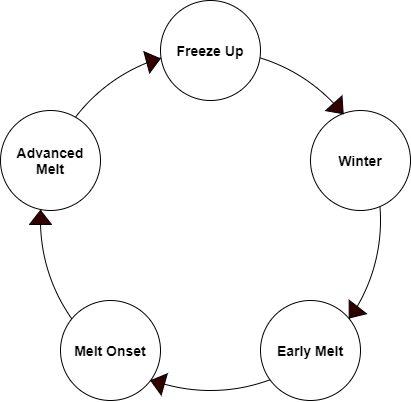
\includegraphics[scale =0.5]{Sea Ice Lifecycle diagram.png}
	\caption{Diagram showing the lifecycle of Antarctic sea ice as observed using remote sensing based on \textcite{barber2005microwave}. The cycle begins with the congealing of the ocean surface known as Freeze Up with peak ice formation during Winter, the second half of the cycle is characterised by various stages of melt with complete sea ice retreat occurring in the Summer.}
	\label{fig:ice_diag}
\end{figure}

Sea ice formation in the Southern Ocean begins when the surface layer of the ocean congeals causing ice crystals to form. These crystals combine to form frazil ice; the concentration of which increases as the heat from the ocean is removed by the atmosphere \cite{arrigo2004large}. As the wind and wave activity begin to calm, frazil ice combines into grease ice, which grows into pancake ice floes \cite{arrigo2004large}. This growth period is known as "freeze-up" and forms the first stages of the sea ice life cycle \cite{barber2005microwave}. Additionally, strong winds in the Marginal Ice Zones cause the floes to drift over long distances \cite{alberello2019drift}. These winds, coupled with high ice floe density result in collisions between floes causing them to break apart \cite{STEER2008933} resulting in brash ice \cite{icedefinition1992}.  During the winter months, newly formed ice grows a layer of snow \cite{barber2005microwave} and is termed "first year ice"\footnote{First year ice is newly consolidated ice that has been growing for less than one winter's growth period \cite{icedefinition1992}.}. Brine is present between the ice fragments and the layer of snow is affected by the level of precipitation \cite{barber2005microwave}.\par

\begin{figure}[H]
	\centering
	\begin{subfigure}[t]{0.5\textwidth}

		 \begin{tikzpicture}
			\node[anchor=south west,inner sep=0] (image) at (0,0) { 		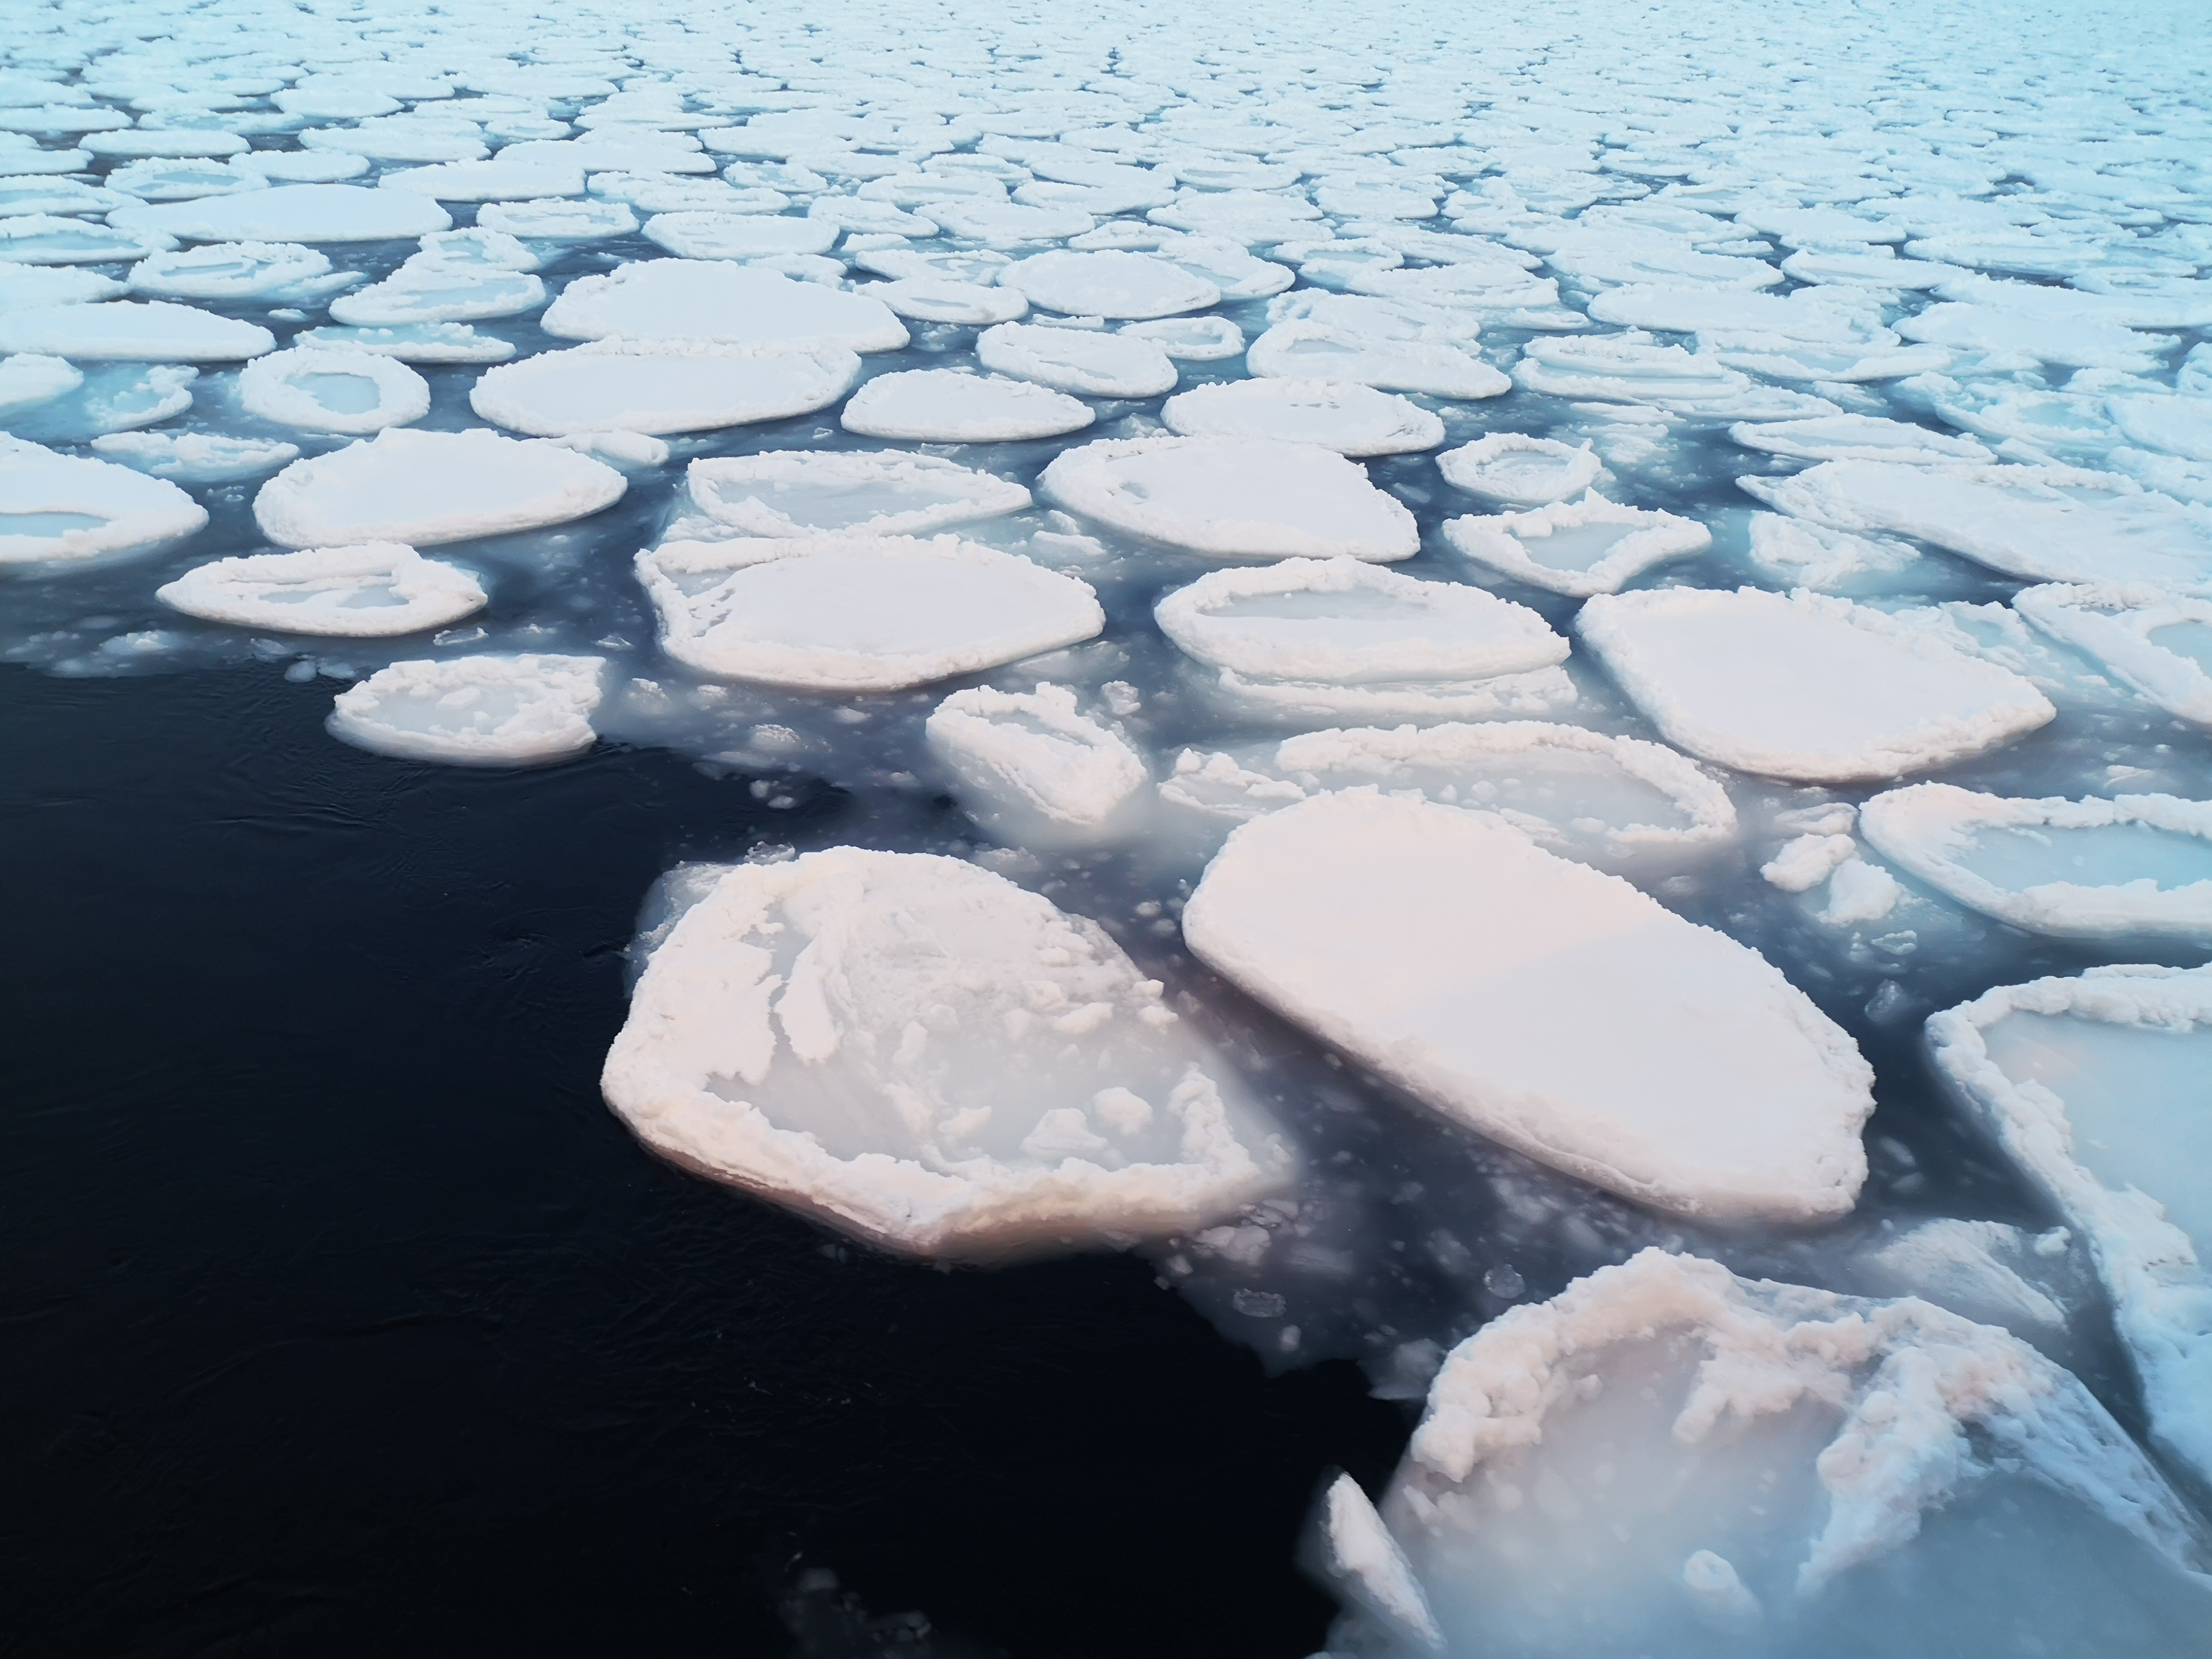
\includegraphics[width = 0.95\linewidth,height=6cm]{floe snow.jpg}};
			\begin{scope}[x={(image.south east)},y={(image.north west)}]
				\draw[color=black, ultra thin,fill=white] (0.0,0.0) rectangle (0.16,0.16) node[pos=.5] {A};
			\end{scope}
		\end{tikzpicture}
	\label{fig:Ice Types}
	\end{subfigure}%
	\begin{subfigure}[t]{0.5\textwidth}
		\begin{tikzpicture}
			\node[anchor=south west,inner sep=0] (image) at (0,0) { 		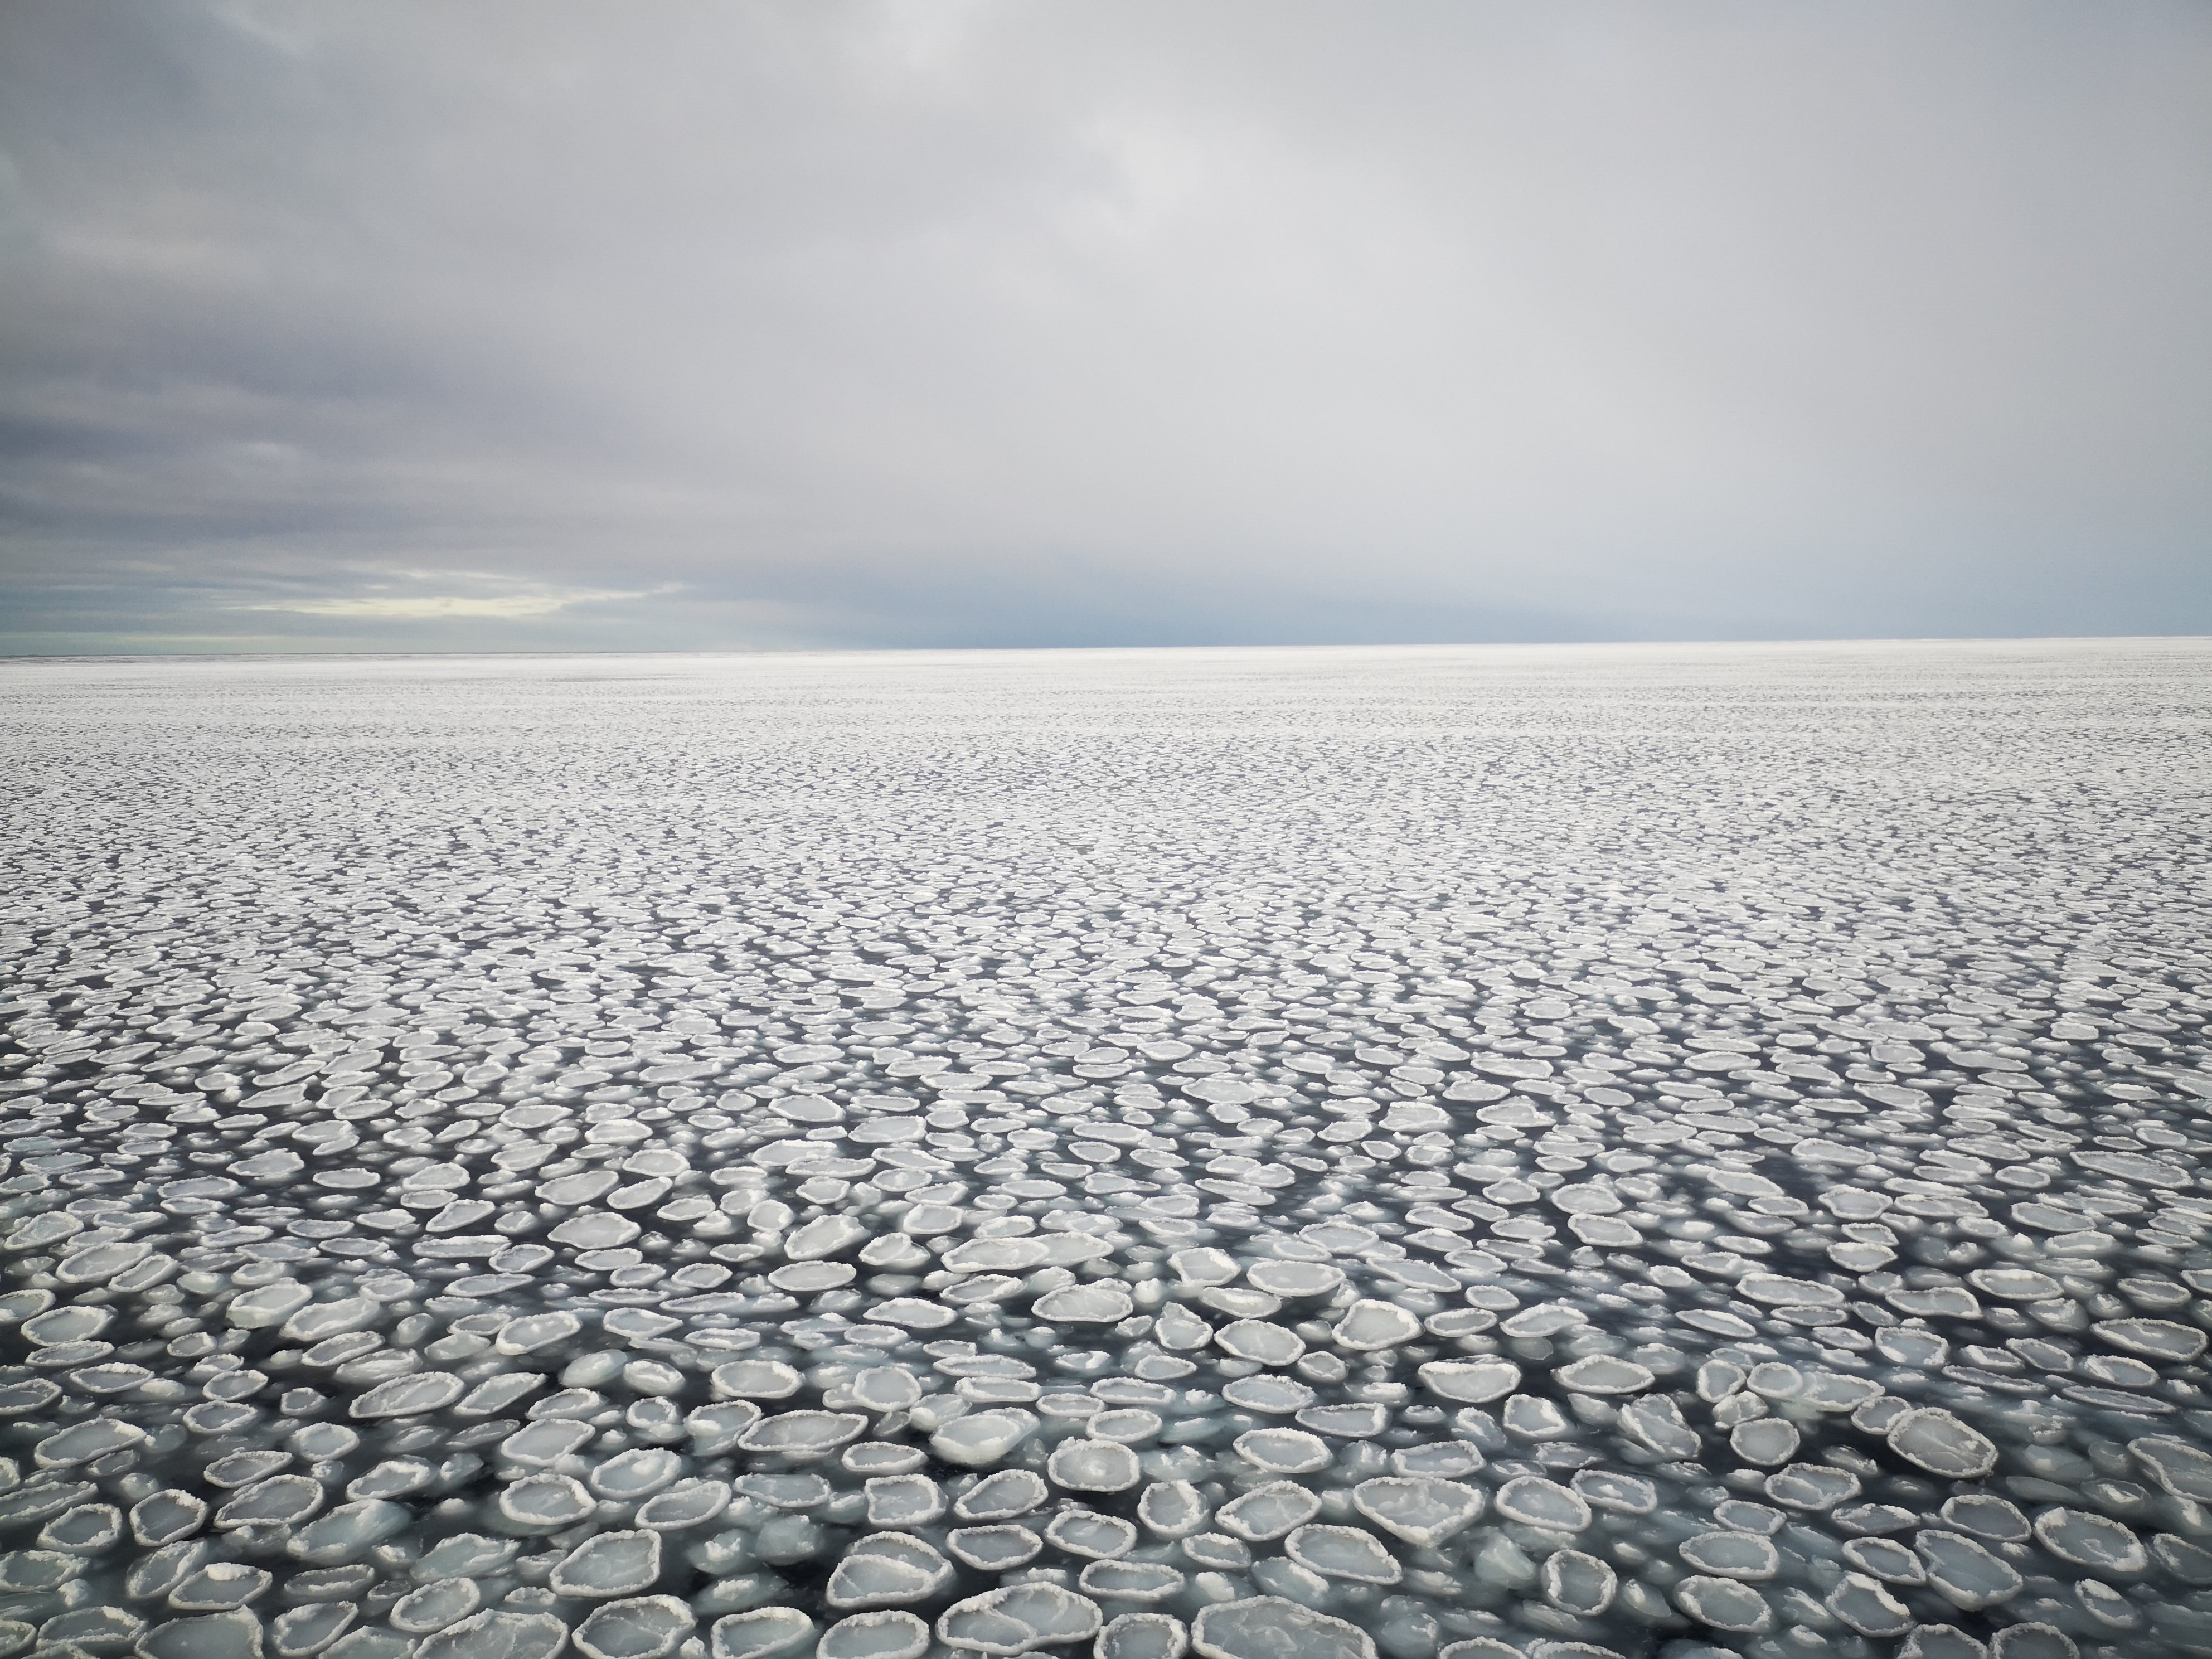
\includegraphics[width = 0.95\linewidth, height = 6cm]{MIZICE.jpg}};
			\begin{scope}[x={(image.south east)},y={(image.north west)}]
				\draw[color=black, ultra thin,fill=white] (-0.01,0.0) rectangle (0.13,0.13) node[pos=.5] {B};
			\end{scope}
		\end{tikzpicture}
		\label{fig:MIZICE}
	\end{subfigure}%
	\caption{(A) Diagram showing different types of ice present in the Marginal Ice Zone including (a) pancake ice floes (b) frazil ice and (c) brash ice. Some ice floes exhibit snow growth along the ridges while other floes exhibit flooding. (B) Sea ice in the Southern Ocean MIZ during July 2019, where pancake ice is the predominant  concentration while brash ice is the smallest. Swell waves can also be observed propagating through the region. Photos taken during the early sea ice formation period during the SCALE winter cruise July 2019 by the author.}
	\label{fig:ridging}
\end{figure}


Finally, the seasonal cycle closes with three phases of melting. Early melt marks the transitional period  where moisture is continuously present in snow cover on the sea ice \cite{barber2005microwave}. The level of moisture in the snow increases through "melt-onset" brought on by the transition from summer to winter and increasing ocean/atmospheric temperatures \cite{barber2005microwave}. Eventually, the snow and ice surface begin to melt rapidly during the "advanced melt" phase resulting in complete desalination of the ice floes followed by the breaking up of the sea ice sheets \cite{barber2005microwave}. 

The result of these processes is a region of semi-consolidated ice, which extends an estimated 19 million $\text{km}^2$ from the Antarctic continent \cite{MAKSYM2012seaiceextent}. These ice floes increase in size through gradual heating, fusing the floes into packed ice \cite{arrigo2004large}. Sea ice concentration in the MIZ covers an observed range of 100\% of total ice concentration from summer to winter \cite{alberello2019drift}. However, \textcite{alberello2019drift} further show that this cover is an unconsolidated mixture of different ice types rather than a single ice cover therefore showing that this metric may not represent the true concentration of sea ice types on a high resolution scale. The variability of the MIZ, coupled with the strong storms and weather patterns, drive the strongest atmospheric-ocean-sea ice interactions in the region. \textcite{alberello2019drift} further highlight that knowledge of MIZ sea ice dynamics is required to model the response to storms as well as predict the regional response to changes in climate.

\begin{figure}[H]
	\centering
	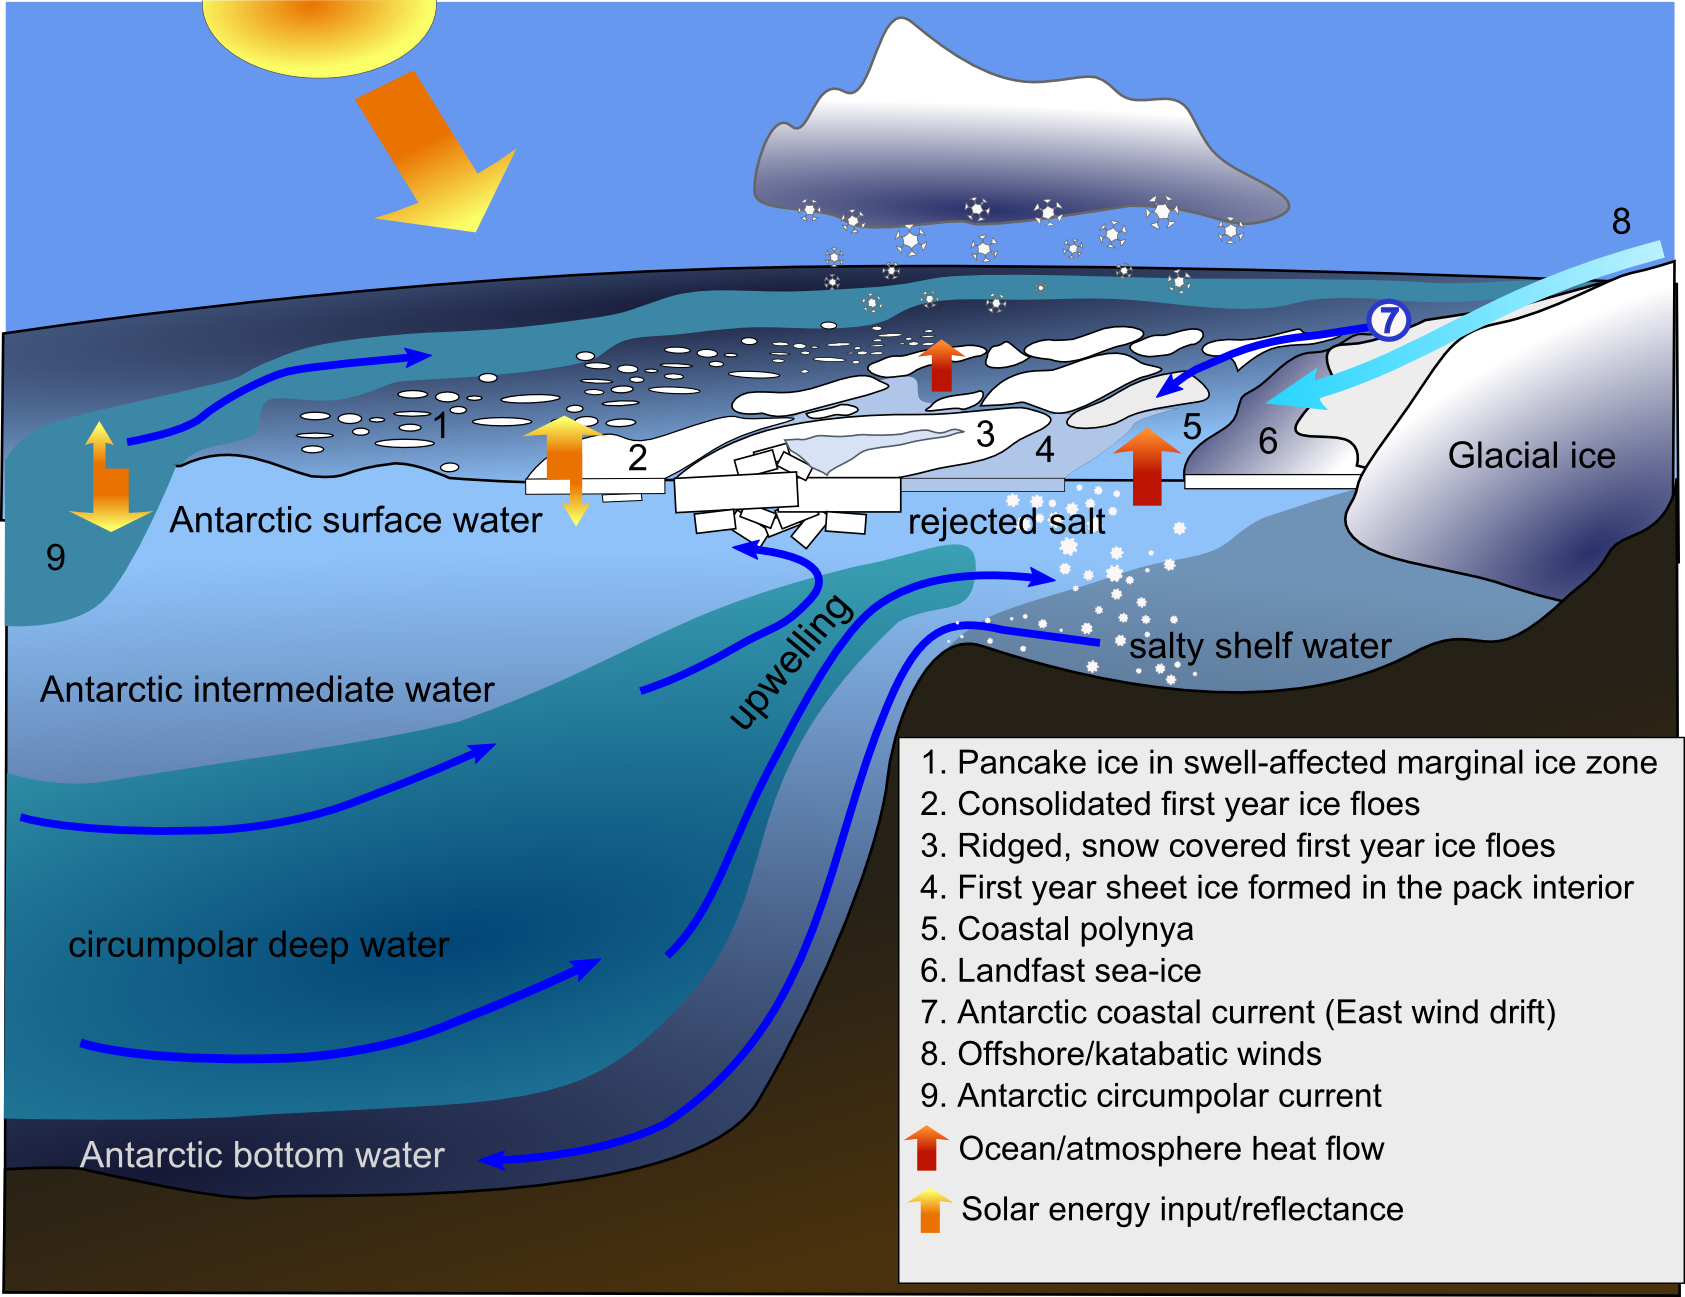
\includegraphics[width = 10cm,height=10cm]{AntDiag.png}
	\caption{Diagram showing the expanse of sea ice in the Southern Ocean. Packed ice forms closer to the continent in calmer conditions while strong oceanic currents, winds, wave action and extreme temperatures result in the formation of semi-consolidated ice in the Marginal Ice Zone (1 to 5). Here, ice formation is highly seasonal expanding to a maximum in winter and retreating to a minimum in summer. Sea ice acts as a boundary layer influencing heat and gaseous  exchange between the atmosphere and ocean. Figure taken from \textcite{Antseaice}.}
	\label{fig:AntaDiag}
\end{figure}

\subsection{Observations of the Marginal Ice Zone}
Antarctic sea ice has gained recognition for playing a critical role in global climate systems \cite{kennicutt2016delivering}. There has been growing interest by the global scientific community in Antarctic Research since the first International Polar Years \cite{kennicutt2016delivering}. International collaborations have sought to formalise Antarctic Research and unite efforts under common goals \cite{kennicutt2016delivering} with the formation of the Scientific Committee on Antarctic Research (SCAR), which has resulted in increased sampling in the MIZ. However, data from the marginal and packed ice zones are under-sampled and poorly represented \cite{vichi2019effects}. Very little in situ data exist to fully understand the environmental conditions surrounding the key metamorphic phases of sea ice in the Antarctic MIZ. Current climate models and observations exist based on data sets from the Arctic \cite{vichi2019effects}, which, when applied to Antarctic sea ice, fail to accurately capture the dynamics of the region on a high-resolution scale. Sea ice expeditions have traditionally taken place during the summer months when the sea ice extent is at a minimum \cite{kennicutt2016delivering}. This results in temporal and spatial gaps in seasonal measurements, which fail to characterise sea ice expanse during the fundamental formation periods \cite{MAKSYM2012seaiceextent}. Additionally, these data are critical for understanding Southern Ocean sea ice dynamics and observed phenomenon in the Marginal Ice Zone such as waves-in-ice \cite{kohout2014storm}. Furthermore, polar oceanic and atmospheric measurements are critical for understanding the local climates since the high cyclonic activity in the region affects the heat and moisture delivery to higher latitudes \cite{vichi2019effects}.

Almost all data collected from in situ measurements in the region are taken during seasonal manned expeditions. Only 22 countries have access and shipping capabilities to initiate expeditions to the region. Additionally, these expeditions require vast resources and complex logistical operations. Furthermore these missions are time sensitive and cancelled expeditions create gaps in seasonal data sets. The harsh seasonal climate causes certain, vital areas of the MIZ and packed ice zones to become inaccessible during winter months. As a result, missions only occur during certain seasons resulting in temporal gaps. Attempts have been made to fill in these gaps using data from Arctic climate programs e.g. \textcite{lee2012program}. However, these attempts fail to characterise the region and accurately capture seasonal variability. For example, in 2016, an anomaly in the sea ice extent was detected where the ice retreated 48\% faster than the mean rate \cite{turner2017unprecedented}. \textcite{vichi2019effects} have shown the region to be a hot-spot for cyclonic activity, which regularly impacts ice formation within the marginal ice zone. However these interactions are not captured by current climate models \cite{vichi2019effects}.\par

\begin{figure}[H]
    \centering
    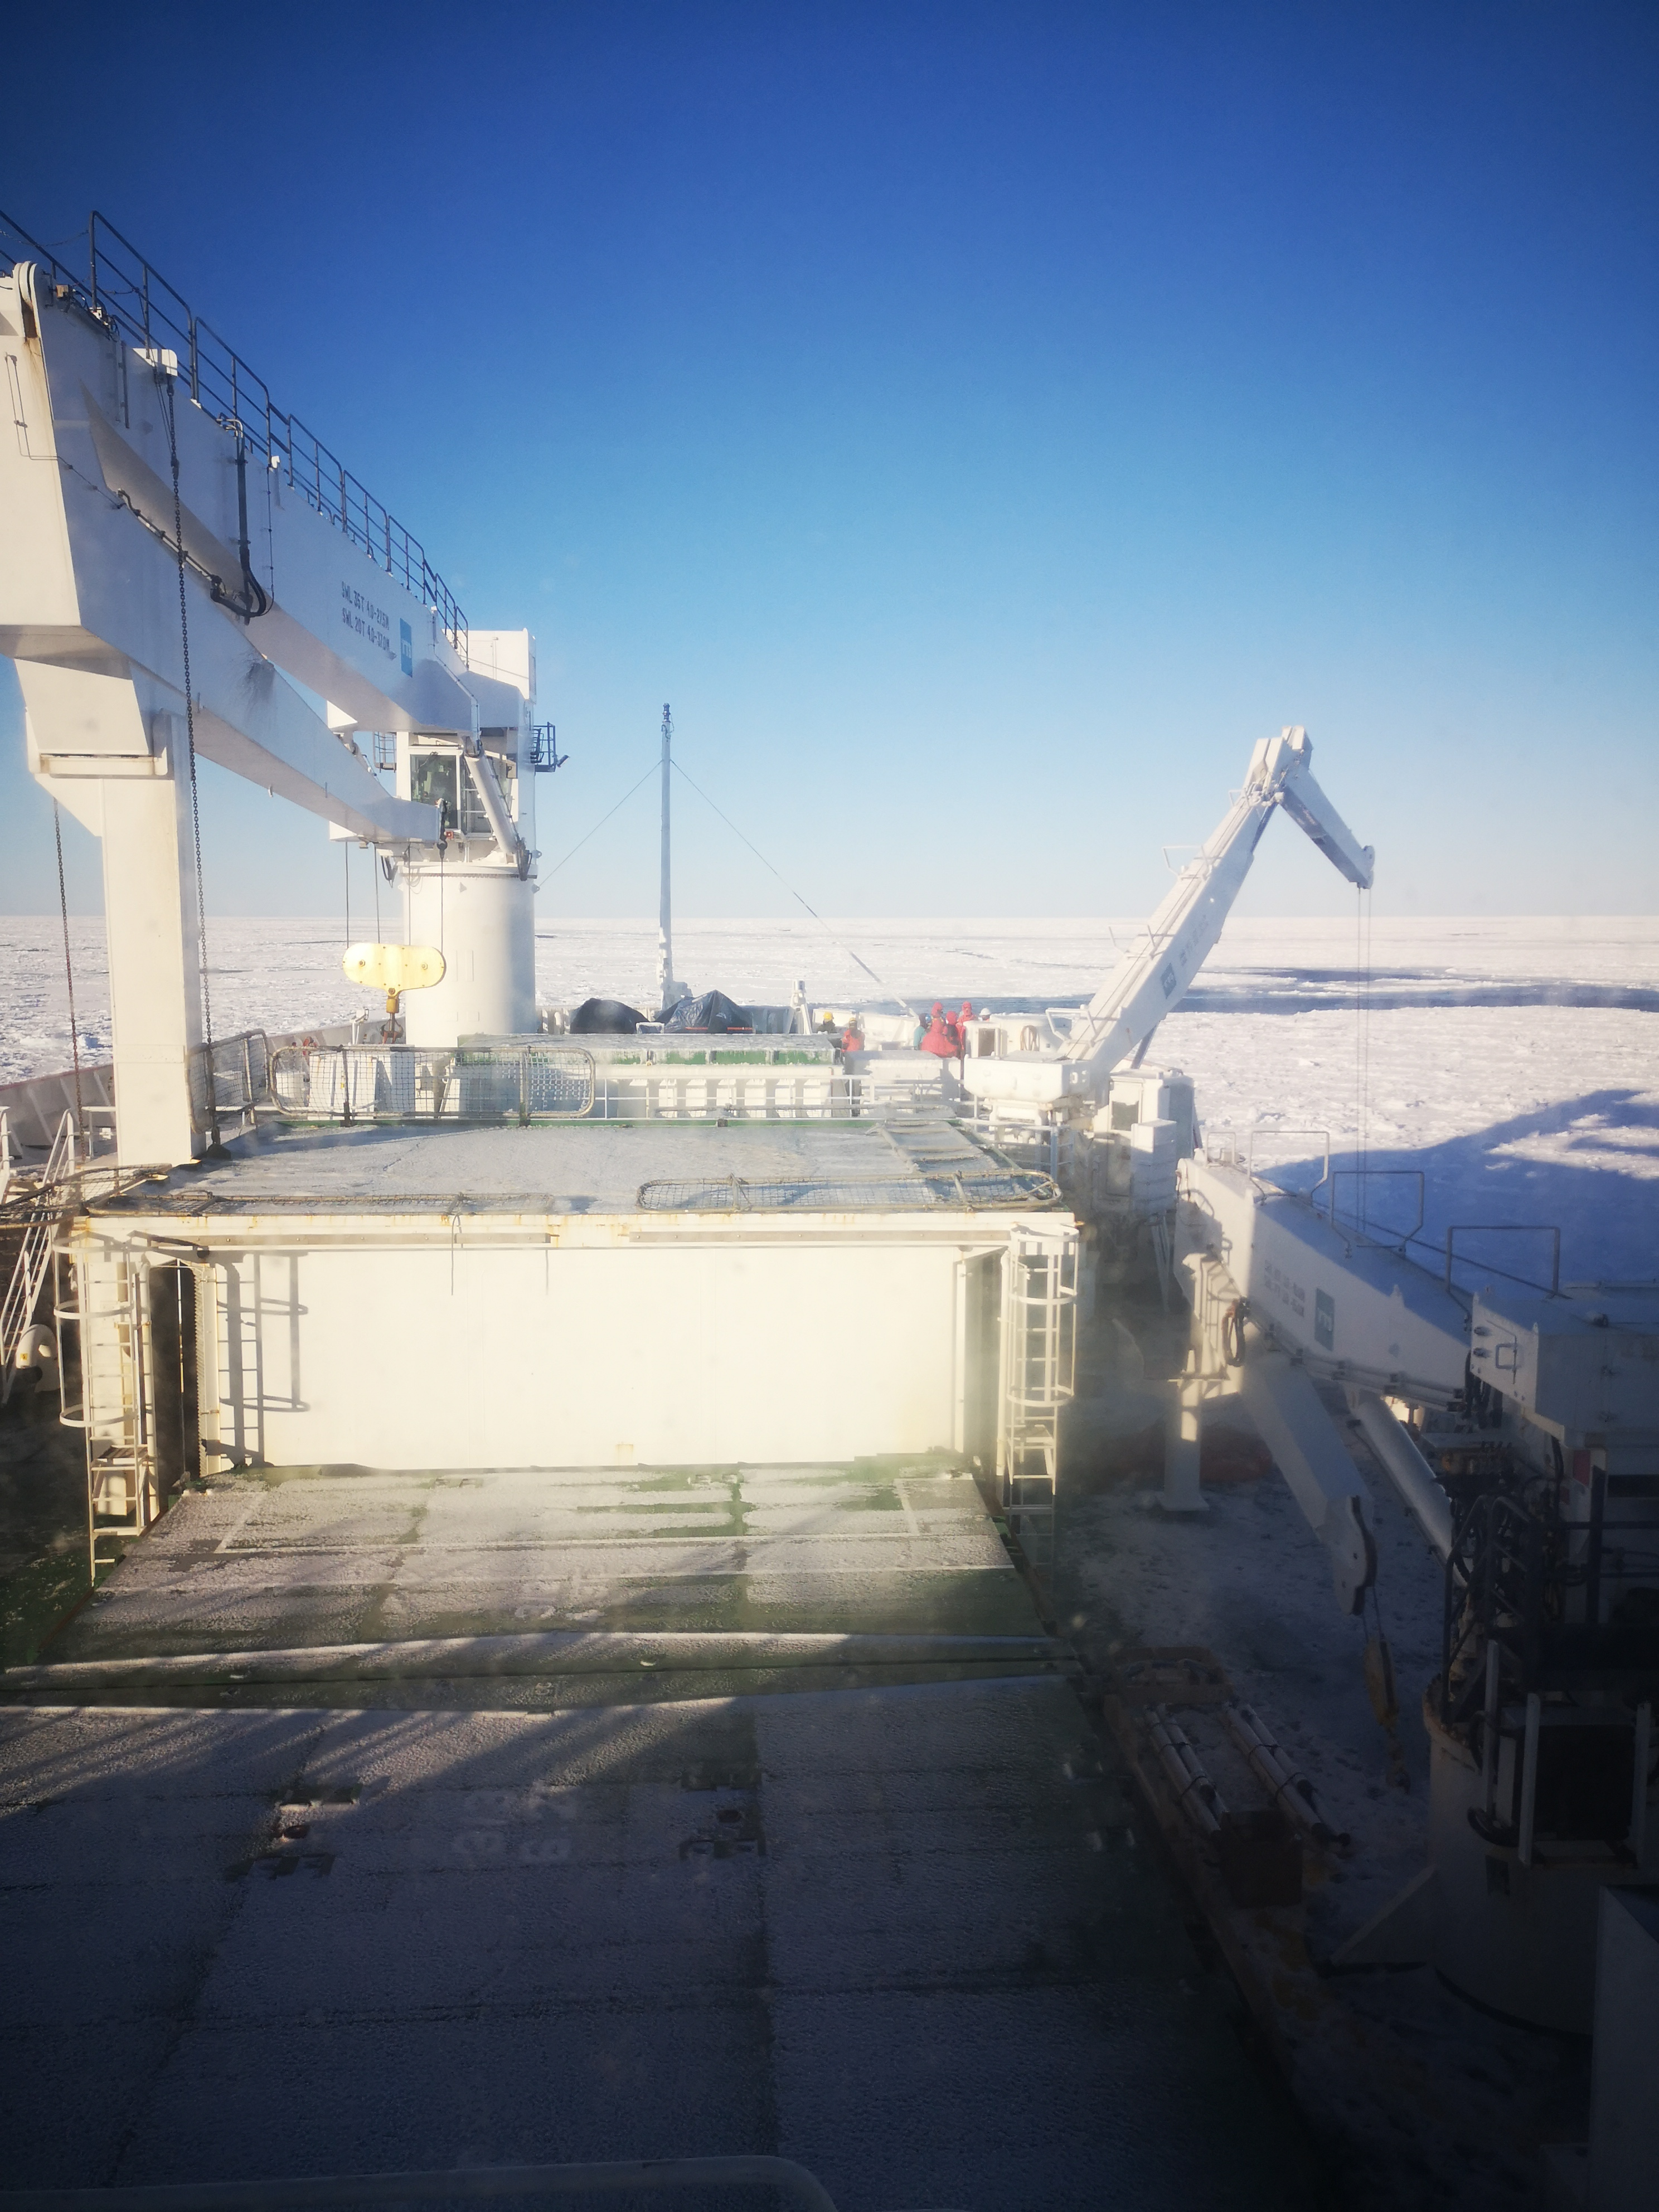
\includegraphics[width = 5cm,height = 7cm]{SHIPACT.jpg}
    \caption{Photo taken in the Marginal Ice Zone from onboard the SA Aghulus II during the SCALE winter expedition in 2019 by the author. The vessel is anchored in consolidated ice with the UCT\protect\footnotemark-UDE\protect\footnotemark sea ice team performing ice coring activities on the surface of the ice.}
    \label{fig:cruise}
\end{figure}
\footnotetext[2]{University of Cape Town}
\footnotetext[3]{University of Duisburg-Essen}

Therefore, a call to increase sensing in the region has arisen to fill in the gaps of these temporal data sets \cite{kennicutt2019sustained}. A review by \textcite{kennicutt2016delivering} highlights a need to revolutionise Antarctic science to overcome these challenges. As part of the plan, SCAR identified technology as playing a pivotal role in Antarctic research. Air, sea and space-borne technologies can replace manned-expeditions which can provide in situ monitoring on a macro and micro scale \cite{kennicutt2016delivering}. Technology can provide a potential solution to long-term monitoring. Robust, power-efficient solutions that are capable of performing long-term functions in a non-invasive manner are required to reduce the need for implementing new infrastructure.\par

\begin{figure}[H]
    \centering
    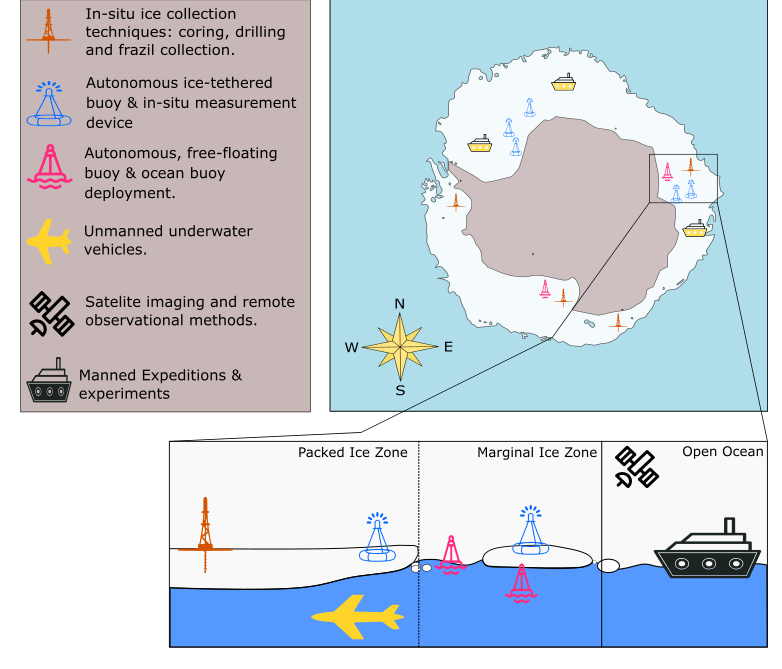
\includegraphics[scale=0.5]{tech.png}
    \caption{ Diagram showing the current state of Antarctic sea ice measurement technologies for each level of observation as well as the estimated deployment location. Diagram taken when sea ice extent is at a maximum. This diagram is derived from the technology implementation strategy identified from the 2016 SCAR roadmap \cite{kennicutt2019sustained}\protect\footnotemark \space and has been adapted to show sea ice observational techniques. }
    \label{fig:chapter1_tech_diag}
\end{figure}

\footnotetext{Figure made using icons from Flaticon.com, Buoy by hunotika from the Noun Project, oil rig by Mourad Mokrane from the Noun Project, Plane by jokokerto from the Noun Project.}

\subsection{Overview of the existing technology and devices}

Modern technology has seen an increased use in remote monitoring of the continent \cite{kennicutt2016delivering}. For example, satellite imaging is the most prevalent technology for monitoring sea ice in both the Arctic and Antarctic regions. It provides large-scale mapping of sea ice extent, thickness, snow cover at  the cost of a low spatial resolution \cite{turner2017unprecedented,galin2011validation,alberello2019drift}. These techniques allowed for the detection of the rapid sea ice retreat recorded in 2016 \cite{turner2017unprecedented} and are very useful for large-scale representation. However, satellite imaging is severely constrained by its resolution \cite{emery1997satellite}. Pixel sizes of synthetic aperture radar (SAR) images are in the order of 10 to 100 m \cite{galin2011validation} where, for example, snow thickness can vary down to the cm. Furthermore, cloud cover can compromise the measurements resulting in missing data. Finally, these measurements require validation against data models, which tend to underrepresent climate in the region \cite{galin2011validation,emery1997satellite}. Hence, a need arises for the development of in situ technology that can provide accurate, detailed information down to the highest possible resolution and allow for long term, large scale monitoring of ocean-ice-atmosphere processes. Hence we turn to autonomous platforms as a solution.\par 
\begin{figure}[H]
    \centering
    \begin{subfigure}[t]{.3\textwidth}
    \begin{tikzpicture}
    \node[anchor=south west,inner sep=0] (image) at (0,0) { 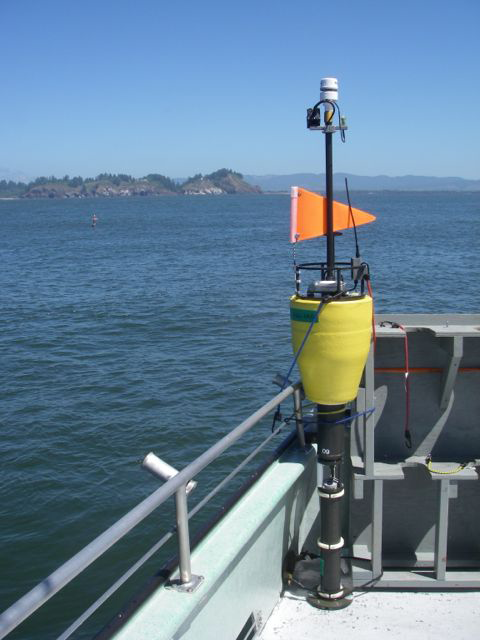
\includegraphics[width = 4cm, height = 6cm]{swift_4.png}};
    \begin{scope}[x={(image.south east)},y={(image.north west)}]
        \draw[color=black, ultra thin,fill=white] (0.0,0.0) rectangle (0.21,0.16) node[pos=.5] {A};
    \end{scope}
    \end{tikzpicture}
    \end{subfigure}
    \hfill
    \begin{subfigure}[t]{.3\textwidth}
        \begin{tikzpicture}
    \node[anchor=south west,inner sep=0] (image) at (0,0) {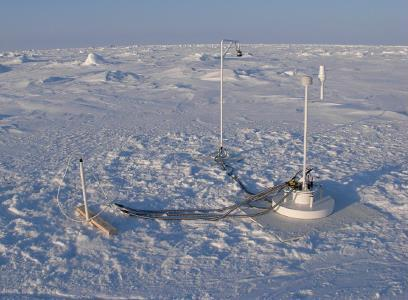
\includegraphics[width = 4cm, height = 6cm]{IMBBuoy1.jpg}};
    \begin{scope}[x={(image.south east)},y={(image.north west)}]
        \draw[color=black, ultra thin,fill=white] (0.0,0.0) rectangle (0.21,0.16) node[pos=.5] {B};
    \end{scope}
    \end{tikzpicture}
    \end{subfigure}
    \hfill
     \begin{subfigure}[t]{.3\textwidth}
      \begin{tikzpicture}
    \node[anchor=south west,inner sep=0] (image) at (0,0) {        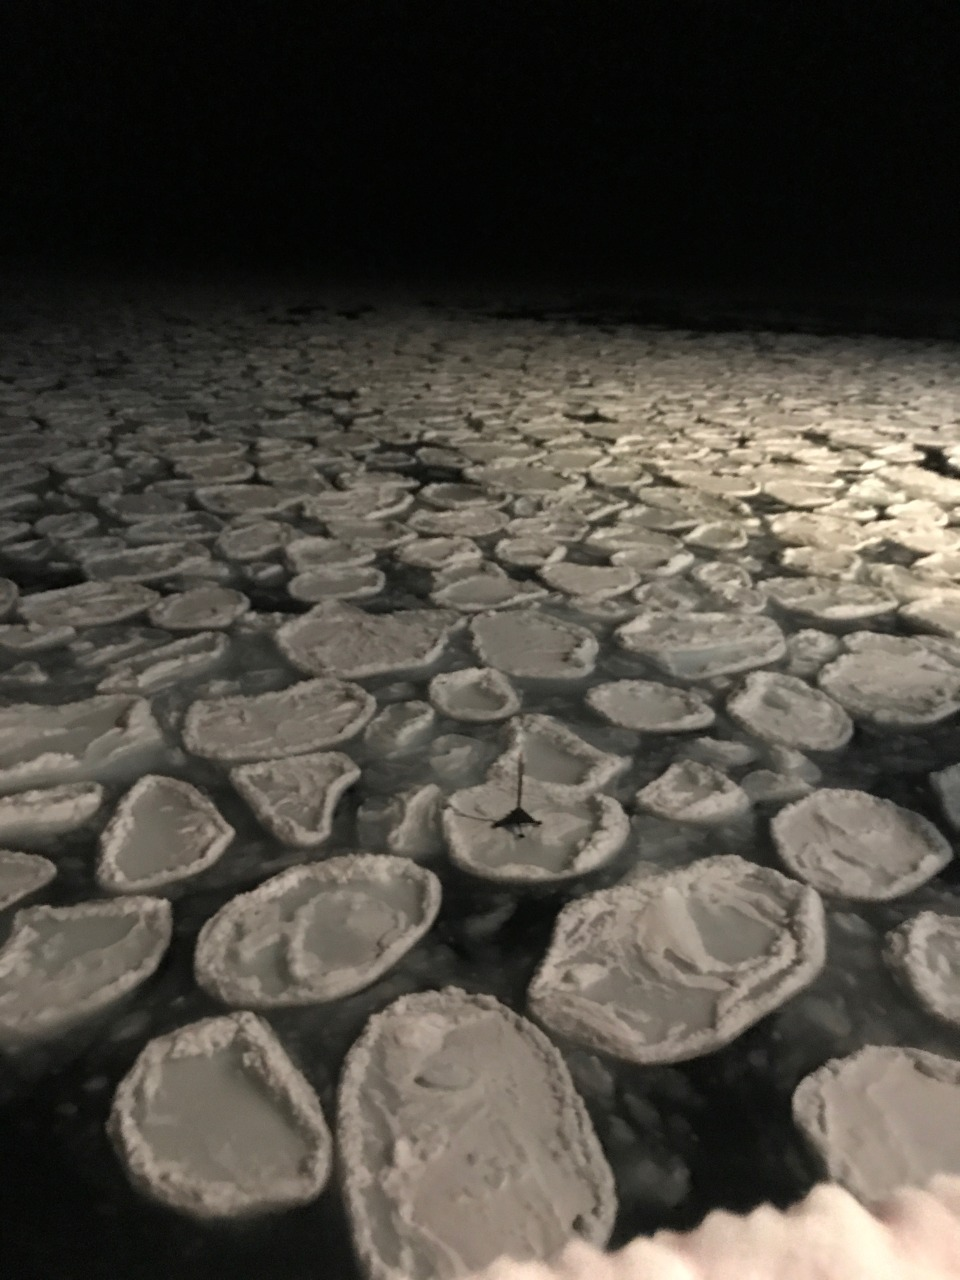
\includegraphics[width = 4cm, height = 6cm]{deploy.jpg}};
    \begin{scope}[x={(image.south east)},y={(image.north west)}]
        \draw[color=black, ultra thin,fill=white] (0.0,0.0) rectangle (0.21,0.16) node[pos=.5] {C};
    \end{scope}
    \end{tikzpicture}
    \end{subfigure}
    \hfill
    \caption{Practical examples of instruments used to collect in situ measurements in the sea ice region. These comprise: (A) the Surface Wave Instrument
Float Tracking (SWIFT) buoy developed by the University of Washington \cite{thomson2012wave}; (B) the Ice Mass Balance (IMB) buoy developed by Dartmouth College [\cite{PLANCK2019102792} image source: \cite{simbfact}]; and (C) the Southern Hemisphere Antarctic Research Collaborative (SHARC) buoy developed by the University of Cape Town (photo courtesy of R. Verrinder).}
    \label{fig:chapter1_prac_buoys}
\end{figure}

Delivering a remote system capable of long-term functionality is a high priority for Antarctic science \cite{kennicutt2016delivering} and will accrue robust, reliable, time-sensitive data-sets to populate these models. This will bring climate models in line with current observations and will allow for a quantified, thorough description of a local phenomenon, for example, the role of ocean swells in ice formation in the Marginal Ice Zone \cite{doble2013wave,doble2017robust}. A successful system should have the following characteristics\footnote{Taken from a collective survey distributed during the Antarctic Roadmap Challenge in 2016 \cite{kennicutt2016delivering}.}: 
\begin{enumerate}

    \item Autonomous or sustained deployment capabilities
    \item Adequate remote sensing capabilities
    \item Improved, robust power supplies
    \item Real-time data collection, transfer and analysis
    \item Survivable under extreme weather conditions
\end{enumerate}

However, the current state of  modern Antarctic observational technology is underdeveloped; current prototypes are too expensive and difficult to obtain by the scientific community \cite{kennicutt2016delivering}. Many institutions have initiated projects to develop autonomous systems such as buoys (examples shown in Figure \ref{fig:chapter1_prac_buoys}) and unmanned surface vehicles (USVs) such as Wave Gliders \cite{liquidrobot2016wave}, which  have been utilised successfully in Antarctic and Arctic oceanographic studies \cite{swart2020submesoscale}. For example, SWIFT buoys deployed in the Arctic Marginal Ice Zone were used to validate Marine Radar measurements of sea ice drift in the Beaufort Sea \cite{lund2018Arctic}. However, these systems are niche and require a technical crew to deploy and retrieve the buoys. The devices are generally proprietary with fixed sets of sensors and fewer sensing capabilities rendering the device inflexible to the needs of scientists \cite{rabault2017measurements}. \textcite{rabault2019open} note the growing use of open source hardware and off-the-shelf technology in modern systems. Off-the-shelf  components have reached a state where the components are well documented and specified to withstand the requirements for polar systems \cite{rabault2019open}. Open-source hardware has allowed for the free exchanging of designs allowing scientists to build their own devices without needing to design and test prototypes \cite{rabault2019open}. As a result, there has been a growth in literature on open access devices with designs and code bases readily available on code sharing sites such as GitHub\footnote{For example: see \textcite{rabault2019open} Github repository at \url{https://github.com/jerabaul29/LoggerWavesInIce_InSituWithIridium}.}. Hence, inclusion of cost-effective technology as a solution is a growing trend. \par 

Additionally, these devices have shown promise in the field. \textcite{rabault2019open} developed an open-source multi-sensing autonomous system and \textcite{kohout2015device} developed a multi-sensing system with off-the components. The devices were deployed in the Arctic and Antarctic Marginal Ice Zones. The buoys developed by \textcite{kohout2015device} encountered technical issues resulting in a total of 39 days survivability with two buoys lost immediately after deployment, one buoy surviving for nine days and another for 17.5 days \cite{kohout2015device}. The devices were deployed again in the Ross Sea by \textcite{kohout_smith_roach_williams_montiel_williams_2020} in April 2020 where a buoy lasted for 66 days \cite{kohout_smith_roach_williams_montiel_williams_2020}. The buoys developed by \textcite{rabault2019open} included solar panels to recharge the batteries. However these systems survived for only 12 days during the spring. Other systems deployed in the region are the MetOcean buoys \cite{uptempo}, Surface Wave Instrument Float Tracking (SWIFT) \cite{thomson2012wave} buoys and Trident buoys \cite{trident}. These systems, however, are expensive and do not have the sensing capabilities specifically for sea ice dynamics. Full details of these remote sensing technologies are discussed in Chapter \ref{ch:chapter2}. Consequently, this presents a problem for in situ sea ice observations in that multiple systems are required to collect desired data for models with a need for back up systems in case of failure. 

Therefore we are presented with a unique opportunity to design a series of novel ice-tethered autonomous systems to increase remote sensing at an affordable rate. The goal of the project is to design a proof of concept system with expandable, modular capabilities capable of running off a single power module for seasonal periods as part of the South African National Antarctic Programme (SANAP), and it is led by the Marine and Antarctic Research centre for Innovation and Sustainability (MARIS) at the University of Cape Town (UCT), in collaboration with the South African Weather Service (SAWS). The focus of this collaboration is to better understand sea ice lifecycle in the Southern Ocean. Hence, the proposed system aims to provide a low-cost, easy to deploy environmental data measurement system that can be expandable to operate in a network allowing for a single-system deployment strategy. In this thesis, the firmware design of a novel ice-tethered buoy for the Antarctic Marginal Ice Zone is presented. The goal is to develop a robust software system  for a platform built using off-the-shelf components to monitor ice drift, atmospheric conditions and waves-in-ice measurements over a full seasonal cycle.

\begin{figure}[H]
    \centering
    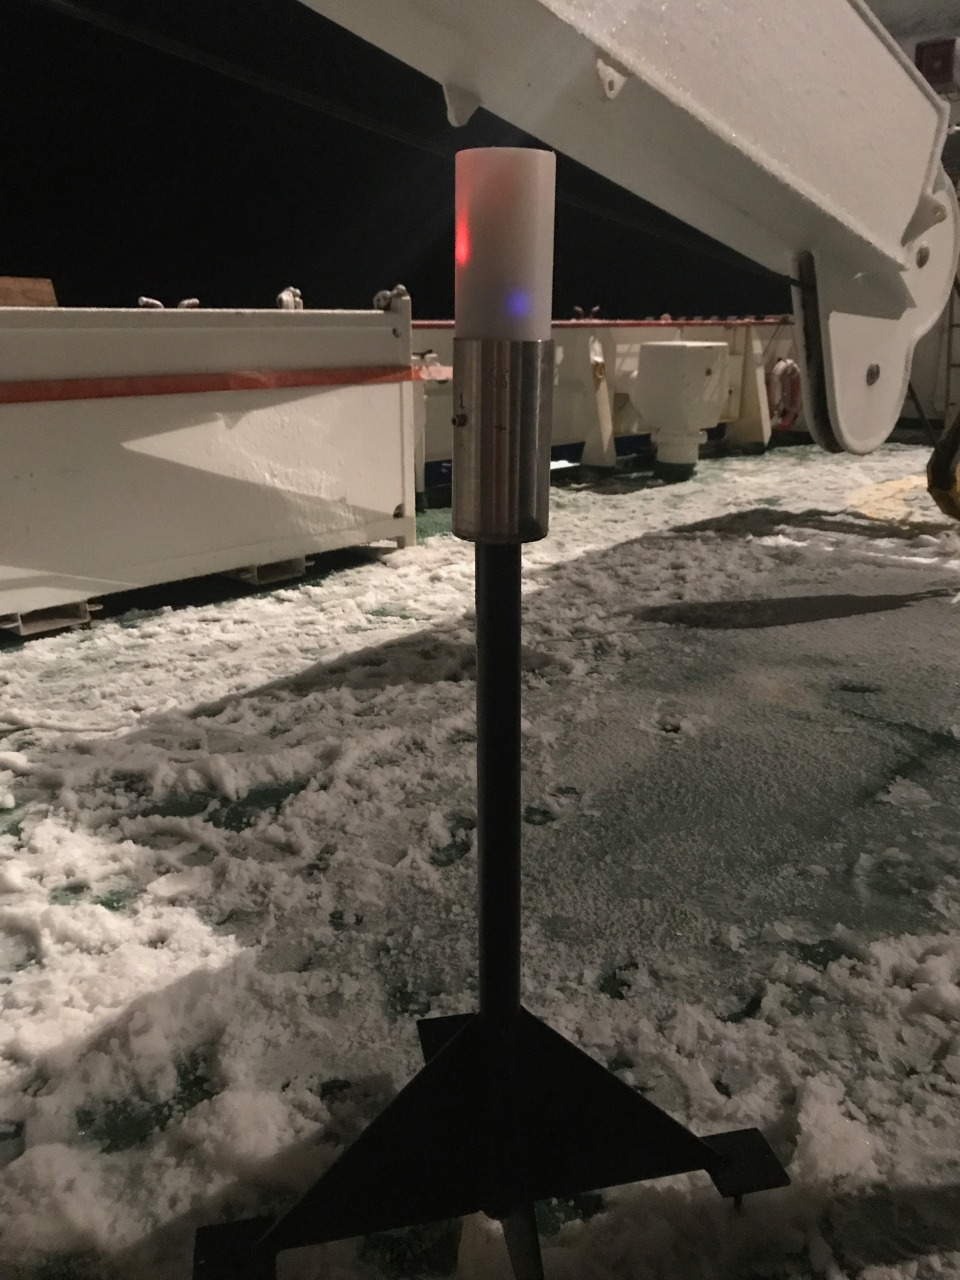
\includegraphics[width = 6cm, height = 8cm]{SHARC.jpeg}
    \caption{Novel ice drift, environmental monitoring and wave measurement autonomous platform: the Southern Hemisphere Antarctic Research Collaboration (SHARC) Buoy. Developed by the University of Cape Town. Photo by R. Verrinder.}
    \label{fig:chapter1_sharc_buoy}
\end{figure}


%====================================================
\section{Problem statement}
\label{subsec:ch1.section2}

This project aims to design a prototype system to monitor environmental conditions that lead to the formation of ice floes in the Marginal Ice Zone. The goal of the project is to increase in situ sensing capability in an affordable manner while allowing for easy access to the technology and data. Conclusion of this project will result in a fully automated system that can be deployed on an ice floe in various locations in the Marginal Ice Zone up to the packed ice boundary layer. Transfer of data from the system will occur using the available infrastructure in the region to reduce costs and make the system as non-invasive as possible. Furthermore, the resulting system will run off a portable power source with limited charging capability to survive for at least one month. By identifying and engaging with key stakeholders in the project, we aim to design a system using off-the-shelf components and synthesise these components into a low-cost, high-performance solution with the final deliverable being a deployable system for the next South African Antarctic expeditions to the Marginal Ice Zone. Thereby creating the following project objectives:
\begin{enumerate}
    \item Perform a literature review of the current state of remote sensing in the Southern Ocean, analysing the techniques and strategies implemented by each system.
    
    \item Engage with key stakeholders to create a set of user requirements for the system, translate these requirements into system specifications, identifying critical subsystems and synthesising them into a high-level system.
    
    \item Identify a suitable network for remote communication as well as the corresponding communication module.
    
    \item Select suitable hardware components and develop a robust set of libraries and unit tests for each system.
    
    \item Identify the energy requirements and select a suitable power source.
    
    \item Identify a processor/set of processors that meet the requirements for the system and develop firmware in C using a Hardware Abstract Layer (HAL).
    
    \item Connect the subsystems to a motherboard and place the system in an enclosure capable of protecting the system from the harsh climate.
     
    \item Evaluate the platform against a serious of unit tests, robustness tests and  hardware tests.
    
    \item Deploy the system in the Marginal Ice Zone and monitor performance.
\end{enumerate}

%----------------------------------------------------

%====================================================

\subsection{Project initiation}

The project was initiated in 2018 with input from the following stakeholders.
\begin{table}[H]
    \centering
    \caption{Legend showing the key stakeholders in the initiation of the project as discussed in the phases below. Legend includes name, reference number and department/institution. }
    \label{tab:proj_init_members}
    \resizebox{\textwidth}{!}{%
    \begin{tabular}{clll}
    \hline
        \textbf{Reference:} & \textbf{Name:} & \textbf{Institution} & \textbf{Department}  \\
        \hline
        \hline
        1 & Jarryd Son & University of Cape Town & Electrical Engineering \\

        2 & Nadir Vorajee & University of Cape Town & Electrical Engineering \\
        
        3 & Prof Amit Mishra & University of Cape Town & Electrical Engineering \\
        
        4 & A/Prof Marcello Vichi & University of Cape Town & Oceanography \\
        
        5 & A/Prof Sebastian Skatulla & University of Cape Town & Civil Engineering\\
        
        6 & Marc de Vos & South African Weather Service & N/A \\
        \hline
        \hline
    \end{tabular}}

\end{table}

\subsubsection{Concept phase}

The concept design was performed by Son (1) and Vorajee (2) under the supervision of Prof Mishra (3). The design was presented at the first meeting on the 11 September 2018 to the principle stakeholders A/Prof Vichi (4) and A/Prof Sebastian Skatulla (5). The proposed device was presented as an upgraded version of the Trident sensing buoy with expanded sensing capabilities. During the meeting, it was agreed to deploy and test the system during the Winter and Spring SCALE expeditions in 2019. The provisional dates for these cruises were: July 2019 and November 2019 respectively. A follow up meeting occurred on the 4th October 2018 where de Vos (6), (South African Weather Service (SAWS)) expressed interest in the research and the development of the project. de Vos (6) provided additional context for the project and presented current work conducted by SAWS.

\subsubsection{Procurement phase}

A preliminary user requirement was conducted by Son and Vorajee (1, 2). From there, suitable components for each of the subsystems were selected with orders being placed on the 19th December 2018. This order included sensors, a u-blox GPS receiver, Zigbee short range communication modules, Rock Seven satellite communication modules, STMicroelectronics STM32F1 microcontroller and inertial measurement units (IMUs).

\subsubsection{Handover phase}

The project was handed over to Jamie Jacobson under the supervision of Robyn Verrinder on the 8th February 2019, officially commencing the prototyping phase of the project.
%----------------------------------------------------

%====================================================
\subsection{Scope}

This thesis focuses on the firmware design for the buoys. The outcome of this study will be a robust set of firmware and unit tests to validate the firmware against. The project timeline takes place from February 2019 to December 2020 with key deliverable dates being:

\begin{enumerate}
    \item 18 June 2019 - SCALE Winter Cruise  (Version 1.0 Complete)
    \item 12 October 2019 - SCALE Spring Cruise (Version 1.0 Revisions)
\end{enumerate}


As this thesis focuses on software development of the project, hardware design is not included in this study and future designs are discussed as recommendations. This includes the mechanical structure and the electronic modules. However, this study includes the selection of devices, which are evaluated against the technical specifications. Additionally, the hardware modules are described.\par 

System testing is conducted on a subsystem software level and the full system. The testing procedures are described in Tables \ref{tab:AT001} to \ref{tab:AT009}. 

Large scale calibrations are not included in the project scope due to tight timeline constraints. Finally, the  design, implementation and calibration of an IMU-based wave measurement algorithm are not explored in this project. The IMU however, will be validated and verified by sampling enough data to fit into a single Iridium transmission packet. 
%----------------------------------------------------

\subsection{Limitations and constraints}

The largest limitation to the project is time constraints. The project timeline coincides with the SCALE research cruise using the winter and spring expeditions for buoy deployment thereby limiting the time frame for development. Additionally, the firmware development is limited to the capabilities of the selected processor. \par 

The firmware development is heavily constrained by the hardware selected for the platform. Peripheral drivers were written for modules that were agreed upon by the project members. Additionally, the IMU, processor, environmental sensor and satellite modem components were pre-selected in 2018. The firmware is thus constrained by design choices originally made in 2018 and early 2019 for the first version of the system. However, these designs were revised for subsequent versions of the buoy from September 2019. As a result of these constraints, the devices were designed without previous knowledge of the environment and with a limited number of sensors.  Finally, the selected processor has a limited number of communication peripherals which influenced the types of sensors that were selected.

The communications network in Antarctica is severely limited and the most reliable form of remote communications is the Iridium satellite network. The amount of data that can be transmitted is limited in terms of bandwidth, data costs, packets structure and reliability of transmission. Testing for Antarctic conditions is restricted by available testing facilities, therefore, rigorous environmental tests may only be conducted during the expeditions.\par 

The first prototype was deployed with a limited number of sensors due to development constraints. Mechanical failures resulted in the buoys ceasing operation within an hour of deployment during the 2019 SCALE Winter cruise. Further development occurred in 2020 to increase the sensing capability of the buoy. However due to the 2020 COVID-19 outbreak, all expeditions were cancelled for the year and therefore final system testing in the Antarctic MIZ was not possible. Attempts were made to deploy the devices on other expeditions from other countries. However, shipping delays were encountered preventing the device from reaching the expedition team on time. Currently, a prototype version has been sent with the SA Agulhas II to the SANAE IV base on the Antarctic continent where testing is expected to take place in late February 2021. This falls outside the time frame of this dissertation. Instead, the buoy will be tested on the home  continent with low temperature tests being conducted in a commercial $-20\degree \text{ C}$ freezer. Currently, two buoys are onboard the RV Polarstern and should be deployed in mid-March 2021 alongside with the Alfred Wegener Institute (AWI) buoys.

\subsection{Assumptions}

The following assumptions were made during the development of the firmware for the buoy. The device has sufficient power to access any of the sub modules if required. Devices that pass a connection test, are considered "online" and capable of producing reliable data. The processors are the Arm-based STMicroelectonics  STM32L4 and STM32F4 microcontrollers and do not come preloaded with any real time/operating system. Development will take place using the Hardware Abstract Layer (HAL) driver files and all hardware that has been selected is rated for the environmental conditions described in Section \ref{sec:ch1.section1}. A system/subsystem is considered valid if it passes a suite of acceptance tests and verified if it meets the functional requirements. Devices that are not active need to be placed in power down mode. Finally, the system is considered complete if it can complete a single measurement cycle from power on without the assistance of any auxiliary equipment.
%----------------------------------------------------

%====================================================
\section{Plan of development}
\label{sec:ch1.section3}

The plan of development describes how the project was conducted through the various stages. A literature review was conducted to analyse the current state of in situ monitoring technology in the region. Then, a problem statement was defined by engaging with project stake holders and developing a set of user requirements. The user requirements were used to formulate acceptance tests and technical specifications which were used to guide subsystem design and selection. Then, the firmware stage was initiated with the development of Application Programming Interface (API) libraries for each module of the device. These were then synthesised and sequenced into a software system defined by short periods of activity and long periods of inactivity. This was used to optimise the device for low power consumption. The system was tested by performing a power consumption test, which was used to evaluate the power characteristics. The device was setup outside to run a full transmission cycle. Finally the results were analysed and used to validate the buoy as a viable tool for remote Antarctic monitoring.
%====================================================
\section{Report structure}
%----------------------------------------------------

\begin{center}
   {\setlength{\extrarowheight}{5pt}%
   	\footnotesize
    \begin{longtable}[H]{>{\centering}m{0.15\textwidth} >{\centering}m{0.2\textwidth}  
   m{0.65\textwidth}}
        \caption{Description of report structure including key phases of the project and
        significance}
        \label{tab:report_structure}\\
        \hline
        \textbf{Chapter} & \textbf{Phase} & \textbf{Description} \\
        \hline
        \hline
        Chapter \ref{ch:chapter2} & Literature review & A description of current sampling techniques using un-manned instrumentation in Polar sea ice research is presented. From this review, the key measurement objectives of each system are identified and an analysis of the state of the art will be used to identify the usefulness and areas where SHARC Buoy can provide a solution. \\
        \hline
        Chapter \ref{sec:ch3_design} to \ref{sec:ch3_FR} & System development &  An analysis of project stakeholders is provided as well as an assessment of their needs. Then, a set of user requirements is developed and ranked in order of importance. The functional requirements selected will guide the device selection and, ultimately, be used to evaluate the performance of the final system. This lead to the identification of the critical subsystems shown in Table \ref{tab:subsys} and a final system topology choice. A set of technical specifications were derived for subsystem hardware selection and a suite of acceptance tests were written to ensure the components conformed to the desired specifications.\\
        \hline
        Chapter \ref{sec:ch3_sysoverview} to \ref{sec:ch3_final_assembly} & Platform overview & A description of the mechanical and electronic components that were selected for the device. The specifications of each component and price are given. The final system consists of a u-blox NEO-7M GPS, Rock SEven RockBLOCK 9603 Iridium modem, Bosch Sensortech BMP28  environmental sensor, TDK InvenSense MPU6050 Inertial Measurement Unit and Texas Instruments INA219 power monitor. Flash chips were selected as a permanent storage solution for data during phases of inactivity. The components were synthesised on a stack of three PCBs shown in Figure \ref{fig:top_elec}. A separate power module is shown in Figure \ref{fig:bot_elec}. An overview on the assembly of the project is given to close the section.\\
        \hline
        Chapter \ref{ch:ch5} & Software overview & A complete overview of the software design process is provided. The key features and focus of the software are outlined along with the firmware structure as shown in Figure \ref{fig:soft_arch}. The project structure includes a breakdown of files, structure and driver files. The configuration of the processor for this application is shown as well as various peripherals and configurations used to set the device up for execution. Then a brief discussion about power mode and system selection ensued to provide clarity on the power-consumption optimisation process. Then a description of the firmware is given. A decision was made to implement a state machine. Here, a finite set of routines were defined and a description of the sequencing was given. Finally an over view of the flow of data from the device to the user was provided.\\
        \hline
        Chapter \ref{sec:ch4_systests} to \ref{sec:ch4_remotedeployment} & Testing & In this section, the tests conducted on the platform and the system are given. These include subsystem acceptance test, full system tests, power tests and preliminary deployment test results from the 2019 SCALE winter expedition.\\
        \hline
        Chapter \ref{sec:ch4_final_eval} & Final evaluation & The results of subsystem acceptance tests are used to validate the system. The outcome of the project is compared to the functional requirements to determine the system's performance and verify that the project goals have been met.\\
        \hline
        Chapter \ref{sec:ch4_disc} & Discussion & This section provides a discussion of the results and key findings. The discussion focuses on the limitations of the power module and the outcome of the power test. Additionally, the performance of the device during the deployment test is discussed. An in-depth analysis of additional subsystem limitations is provided along with the performance of the firmware in spite of these limitations. The section concludes with a comparison of the buoy against other devices in the field.\\
        \hline
        Chapter \ref{ch:conclusion} & Conclusion &  The outcome of the project is presented and a conclusion is made about the project outcomes, goals and whether the firmware was able to achieve them.\\
        \hline
        Chapter \ref{ch:recommendations} & Recommendations & Improvements and recommendations are provided for future work on the project. These include tests that could not be conducted, research and focus areas as well as hardware/software improvements. \\
        \hline
        \hline
    \end{longtable}}

\end{center}
    
%****************************************************
% END
%****************************************************


\chapter{Literature Review}
\label{ch:chapter2}
As highlighted by section \ref{sec:ch1.section1}, there is a great desire by research scientists for in situ instruments to provide observation data which fills spatial and temporal measurement gaps in Antarctic sea ice monitoring in the Southern Ocean as shown in figure \ref{fig:Antarctica_Southern_Ocean}. This chapter investigates the current use of autonomous monitoring technology used by research scientists in this region focusing on progress made to improving in situ observations and highlighting areas for improvement.

\begin{figure}[H]
	\centering
	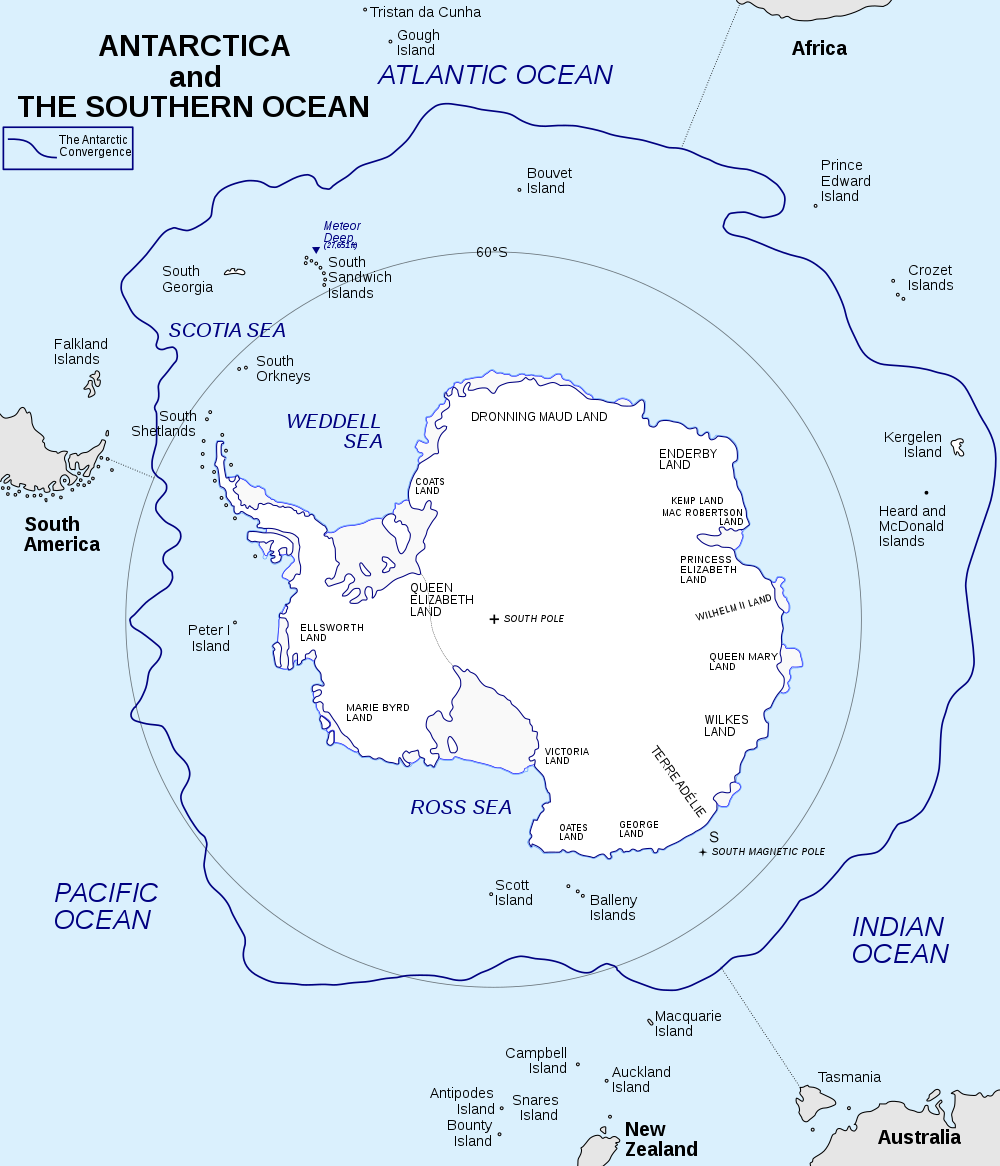
\includegraphics[width = 10cm,height=10cm]{Antarctica_and_the_Southern_Ocean.png}
	\caption{Map of the Southern Ocean surrounding the Antarctic continent. Image created by \textcite{Hogweed2015Ocean} and licensed by CC BY-SA 3.0}
	\label{fig:Antarctica_Southern_Ocean}
\end{figure}


%%%%%%%%%%%%%%%%%%%%%%%%%%%%%%%%%%%%%%%%%%%%%%%%%%%%%%%%%%%%%%%%%%%%%%%%%%%

\newpage
\section{In situ climate sensing technologies}

Autonomous instrumentation has seen increased use for in situ observations in the polar sea ice regions \cite{kennicutt2016delivering}. These devices have typically  been developed by the commercial sector \cite{rabault2017measurements} from companies such as Trident \cite{trident}, MetOcean \cite{uptempo}, Seabird \cite{seabird2021website} and Sea Technology Services (STS) \cite{sts2021website}. Additionally, academic institutions have also developed in situ measurement devices such as The University of Washington's SWIFT buoy \cite{thomson2012wave} or University of Dartmouth's Seasonal Ice Mass Balance (SIMB) buoy \cite{polashenski2011seasonal}. While these technologies have the benefit of reliability, they are often expensive \cite{rabault2017measurements} and inflexible to the specific needs of polar scientists. Technology has reached a point where low-cost and open source alternatives are well documented and reliable enough to be integrated into customized solutions \cite{rabault2019open}.\par 

\begin{figure}[H]
	\centering
	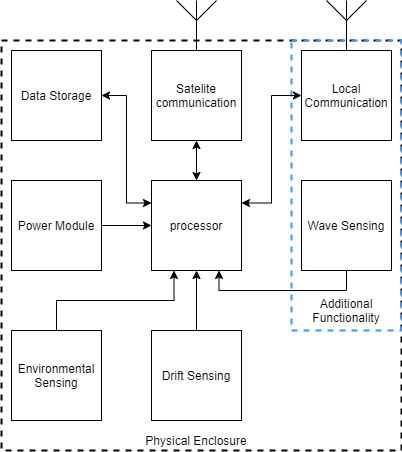
\includegraphics[width = 0.5\linewidth]{device block diagram.png}
	\caption{A block diagram of a typical device for in situ measurements. Each device contains modules for environmental sensing and drift sensing connected to a processor. This can be a micro-controller or microprocessor. Additionally, a data storage module (such as an SD card) is included to store data during the operation. Some device include modules for local communications or wave sensing units. Finally, a remote communication module is included to transfer the data to a research center or a user. The electronics are placed inside a physical enclosure for protection against the polar climate while a portable power module supplies the device during its operation.}
	\label{fig:devblockdiag}
\end{figure}

In this section, a comparison of data collection devices used in the polar regions is presented as well as  description of their design, opperation and deployment. Where possible, certain specifications have been converted into standardised formats. To ensure a fair evaluation, data were collected from the latest technical publication of each platform where possible. These publications may not contain all relevant data. In this case, the data entry has been marked with a "Not reported" or "NR". Figure \ref{fig:buoys}.


Eight platforms were selected for the comparison with each device designed by a private company or an institution. The key collaborators as well as the name of the institution are provided in table \ref{tab:device_list}. Where a buoy name is not given, the device will be named after the key contributor to the project. These systems have been selected due to their prevalence in global polar/ oceanographic science as well as notability in publications. Device performance will be evaluated in the context of the requirements set out by \textcite{kennicutt2016delivering} for an autonomous in situ measurement device shown in section \ref{sec:ch1.section1}. 

\label{ch2:secdevice}
\begin{figure}[H]
	\centering
	\begin{subfigure}[b]{0.24\textwidth}
		\centering
		\begin{tikzpicture}
			\node[anchor=south west,inner sep=0] (image) at (0,0) { 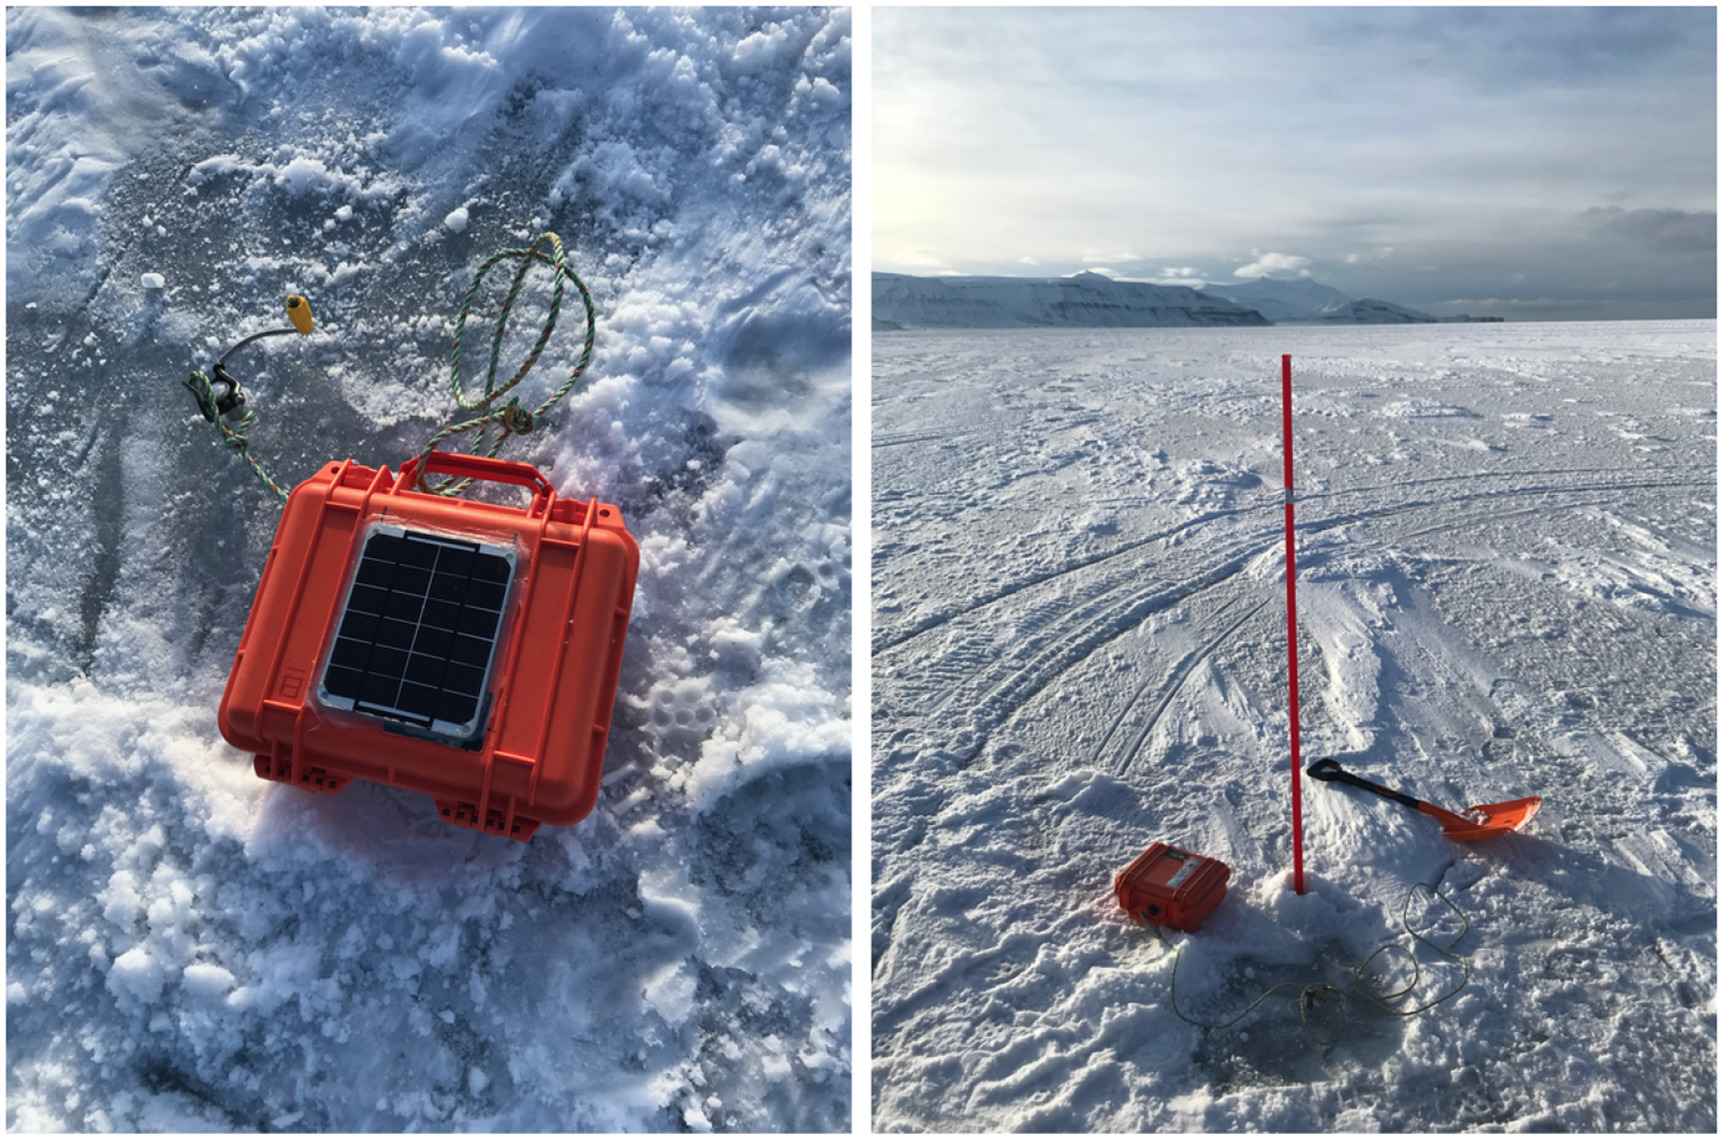
\includegraphics[width = 4cm,height=4cm]{WIIB.jpg}};
			\begin{scope}[x={(image.south east)},y={(image.north west)}]
				\draw[color=black, ultra thin,fill=white] (0.0,0.0) rectangle (0.21,0.16) node[pos=.5] {A};
			\end{scope}
		\end{tikzpicture}
		\label{fig:WIIB}
	\end{subfigure}%
	\hfill
	\begin{subfigure}[b]{0.24\textwidth}
		\centering
		\begin{tikzpicture}
			\node[anchor=south west,inner sep=0] (image) at (0,0) { 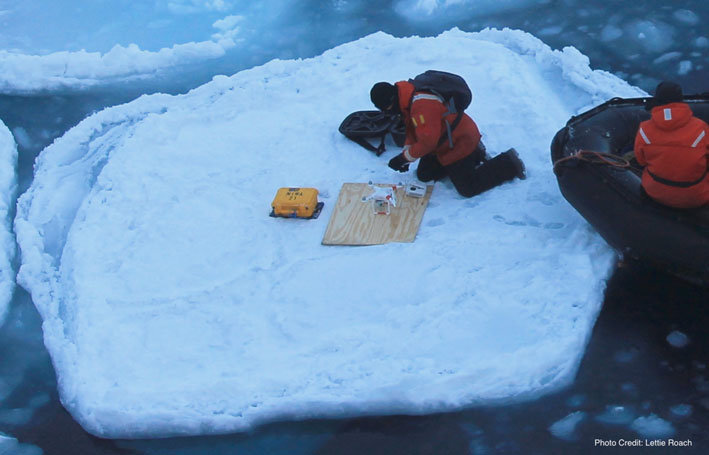
\includegraphics[width = 4cm,height=4cm]{WIIOS.png}};
			\begin{scope}[x={(image.south east)},y={(image.north west)}]
				\draw[color=black, ultra thin,fill=white] (0.0,0.0) rectangle (0.21,0.16) node[pos=.5] {B};
			\end{scope}
		\end{tikzpicture}
		\label{fig:WIIOS}
	\end{subfigure}%
	\hfill
	\begin{subfigure}[b]{0.24\textwidth}
		\centering
		\begin{tikzpicture}
			\node[anchor=south west,inner sep=0] (image) at (0,0) { 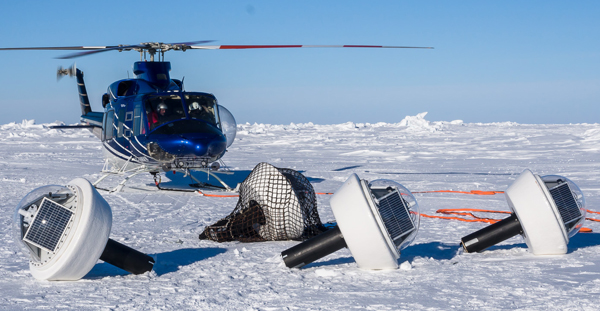
\includegraphics[width = 4cm,height=4cm]{doble.jpg}};
			\begin{scope}[x={(image.south east)},y={(image.north west)}]
				\draw[color=black, ultra thin,fill=white] (0.0,0.0) rectangle (0.21,0.16) node[pos=.5] {C};
			\end{scope}
		\end{tikzpicture}
		\label{fig:NDWB}
	\end{subfigure}%
	\hfill
	\begin{subfigure}[b]{0.24\textwidth}
		\centering
		\begin{tikzpicture}
			\node[anchor=south west,inner sep=0] (image) at (0,0) { 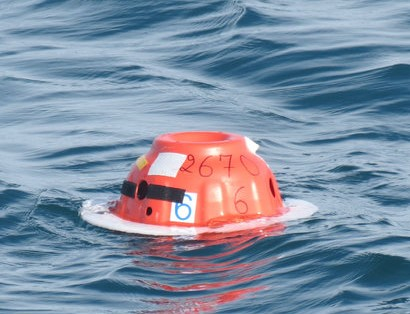
\includegraphics[width = 4cm,height=4cm]{SKIB.png}};
			\begin{scope}[x={(image.south east)},y={(image.north west)}]
				\draw[color=black, ultra thin,fill=white] (0.0,0.0) rectangle (0.21,0.16) node[pos=.5] {D};
			\end{scope}
		\end{tikzpicture}
		\label{fig:SKIB}
	\end{subfigure}%
	\hfill
	\begin{subfigure}[b]{0.24\textwidth}
		\centering
		\begin{tikzpicture}
			\node[anchor=south west,inner sep=0] (image) at (0,0) { 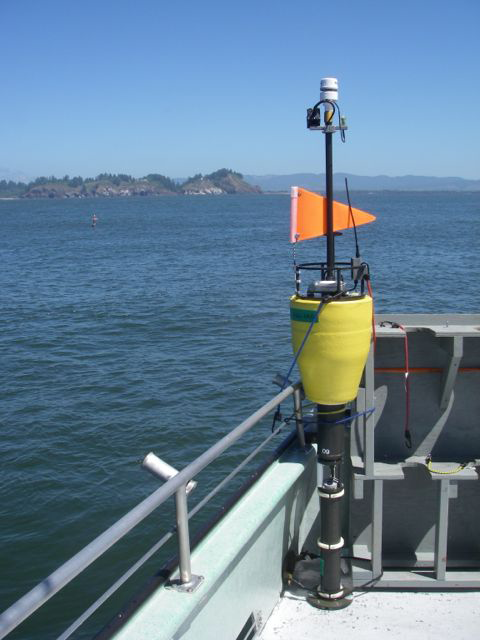
\includegraphics[width = 4cm,height=4cm]{swift_4.png}};
			\begin{scope}[x={(image.south east)},y={(image.north west)}]
				\draw[color=black, ultra thin,fill=white] (0.0,0.0) rectangle (0.21,0.16) node[pos=.5] {E};
			\end{scope}
		\end{tikzpicture}
		\label{fig:SWIFT}
	\end{subfigure}%
	\hfill
	\begin{subfigure}[b]{0.24\textwidth}
		\centering
		\begin{tikzpicture}
			\node[anchor=south west,inner sep=0] (image) at (0,0) { 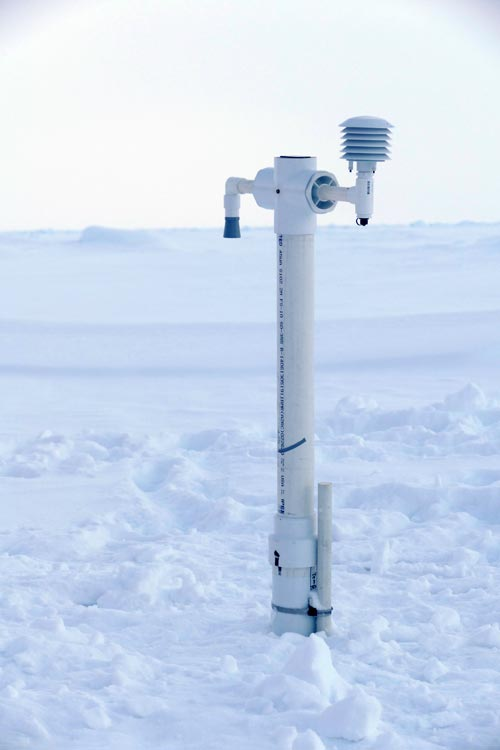
\includegraphics[width = 4cm,height=4cm]{SIMB.jpg}};
			\begin{scope}[x={(image.south east)},y={(image.north west)}]
				\draw[color=black, ultra thin,fill=white] (0.0,0.0) rectangle (0.21,0.16) node[pos=.5] {F};
			\end{scope}
		\end{tikzpicture}
		\label{fig:SIMB}
	\end{subfigure}%
	\hfill
	\begin{subfigure}[b]{0.24\textwidth}
		\centering
		\begin{tikzpicture}
			\node[anchor=south west,inner sep=0] (image) at (0,0) { 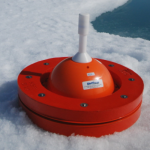
\includegraphics[width = 4cm,height=4cm]{UptempO.png}};
			\begin{scope}[x={(image.south east)},y={(image.north west)}]
				\draw[color=black, ultra thin,fill=white] (0.0,0.0) rectangle (0.21,0.16) node[pos=.5] {G};
			\end{scope}
		\end{tikzpicture}
		\label{fig:UptempO}
	\end{subfigure}%
	\hfill
	\begin{subfigure}[b]{0.24\textwidth}
		\centering
		\begin{tikzpicture}
			\node[anchor=south west,inner sep=0] (image) at (0,0) { 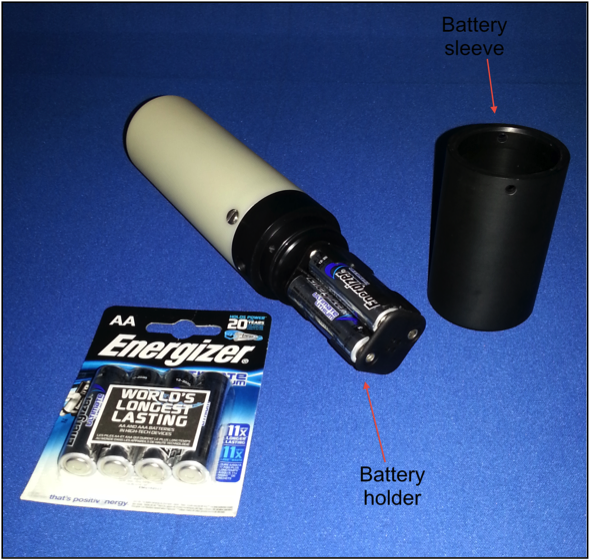
\includegraphics[width = 4cm,height=4cm]{trident.png}};
			\begin{scope}[x={(image.south east)},y={(image.north west)}]
				\draw[color=black, ultra thin,fill=white] (0.0,0.0) rectangle (0.21,0.16) node[pos=.5] {H};
			\end{scope}
		\end{tikzpicture}
		\label{fig:trident}
	\end{subfigure}%
	\hfill
	\caption{ Devices used for the comparison of autonomous instruments deployed in the sea ice region. Each device has been selected for its notability in published work as well as prevalence in sea ice and wave interactions in the Marginal Ice Zones. These devices are: (A) Wave in Ice Buoy developed by \textcite{rabault2017measurements} \cite{rabault2017measurements}, (B) Wave in Ice Observational System by \textcite{kohout2015device} \cite{kohout2015device}, (C) Novel Wave Directional buoys by \textcite{doble2017robust} \cite{doble_wave_2015}, (D) Surface Kinematic buoy by \textcite{guimaraes2018surface} \cite{guimaraes2018surface}, (E) Surface Wave Instrument Float Tracking buoy by \textcite{thomson2012wave}  \cite{jim_swift_2012}, (F) Seasonal Ice Mass Balance buoy by \textcite{polashenski2011seasonal} \cite{simbpic}, (G) Polar ISVP  by MetOcean \cite{uptempo}, (H) Trident buoy by Trident \cite{trident}.}
	\label{fig:buoys}
\end{figure}


A device that has sufficient autonomous and sustained capabilities will operate remotely with no human intervention. Therefore, the operating period of each device will be compared. This is the period between deployment and final transmission where the buoy is active. Additionally, the techniques for remote communication for each buoy will be examined in terms of data rates, coverage and transmission strategy to determine the techniques used to achieve remote communication effectively including a brief over view of available satellite networks. Then, to measure the sensing capabilities of each device, the measurement objectives of each device will be discussed as well as the hardware modules and software used to determine information. To compare the real time data collection, transfer and analysis, the device's processing strategy and storage strategies will be discussed. Data transfer techniques will be analysed with the remote communication section. Finally, device performance in the polar regions will be discussed through the success of each deployment, device deployment time, data integrity will be compared as well as devices that failed and the causes of those failures.

\begin{center}{\setlength{\extrarowheight}{5pt}%
		\begin{longtable}[H]{|>{\RaggedRight}m{0.3\textwidth}|>{\RaggedRight}m{0.2\textwidth}| >{\RaggedRight}m{0.4\textwidth}|}
			\caption{Devices used for the comparison including the device name, lead developer and the institution. These consist of both commercial and institutional devices for in-situ sea ice and wave measurements.}\\
			\hline
			\label{tab:device_list}
			\textbf{Device Name} & \textbf{Developed By} & \textbf{Institution}\\
			\hline
			Waves in Ice Buoy (WIIB) & Jean Rabault & University of Oslo, Norway \cite{rabault2019open} \\
			\hline
			Waves in Ice Observational System (WIIOS) & Alison Kohout & National Institute of Water and Atmospheric Research \cite{kohout2015device}, New Zealand \\
			\hline
			Novel Directional Wave Buoys (NDWB) & Martin J Doble &  Polar Scientific (Ltd.), United Kingdom \cite{doble2017robust}\\
			\hline
			Surface Kinematic Buoy (SKIB) & Pedro Veras Guimarães & Université de Bretagne Occidentale, France \cite{guimaraes2018surface} \\
			\hline
			Surface Wave Instrument Float with Tracking (SWIFT) Buoy & Jim Thompson & University of Washington Applied Physics Laboratory, United States of America \cite{thomson2012wave}\\
			\hline
			Seasonal Ice Mass Balance Buoy (SIMB) & Donald K. Perovich & Dartmouth College \\
			\hline
			Polar ISVP & MetOcean & MetOcean \\
			\hline
			UptempO & MetOcean & MetOcean \\
			\hline
			Trident Buoy & Trident Sensor & Trident Sensor \\
			\hline
		\end{longtable}
	}
\end{center}


\section{System Level Overview}

\subsection{Remote Communication}
\label{ch2:sec_remote}

On the Antarctic continent, remote communication is critical for ongoing scientific activities allowing for data to be transmitted from instruments to research stations and camps \cite{Sanghyun2016satellite}. These activities are further supported by high speed, high bandwidth communication networks such as fibre links \cite{jabbar2001multi} however, these networks have been implemented on a small scale to support permanent field camps \cite{Sanghyun2016satellite} on the continent. \textcite{Sanghyun2016satellite} show that communication from polar stations and field sensors to the rest of the world occurs using satellite constellation networks \cite{Sanghyun2016satellite}. These constellations are classified as  geostationary earth orbit such as Inmarsat \cite{inmarsat2021website} and Intelsat \cite{intelsat2021website} or low earth orbit (LEO) such as ORBCOMM \cite{orbcomm2021website}, Iridium \cite{iridium2019website}, Globalstar \cite{globalstar2021website} \cite{jabbar2001multi}. GEO satellites consist of 2 - 8 satellites orbiting the equator \cite{jabbar2001multi}. As a result, the network coverage is strong for mid-latitudes and weak for low latitudes. However, these satellites cover large areas providing longer connectivity (of up to 6.5 hours) \cite{Sanghyun2016satellite}. LEO satellites cover less surface area and have a smaller connectivity window (10 - 30 minutes). However, these constellations consist of more satellites. Additionally, the Iridium satellite network is the only LEO network that reaches the polar region \cite{jabbar2001multi} and allow for longer network connectivity. The constellation consists of 66 satellites \cite{Sanghyun2016satellite} and is well optimised for marine applications making it suitable for Southern Ocean sea ice applications. Iridium is a satellite network with global coverage and a variety of modems for various IoT uses. The company offers four main data services. Each service places constraints on the data transmission rates, bandwidth and modem selection. Each modem runs a data service that dictates the transmission rates, bandwidth and protocols.  Table \ref{tab:iridium service} shows the available network services. Furthermore, a full description of these modems is shown in table \ref{tab:ir_devices}. \par 

\begin{figure}[H]
	\centering
	\begin{subfigure}[b]{0.3\textwidth}
		\begin{tikzpicture}
			\node[anchor=south west,inner sep=0] (image) at (0,0) { 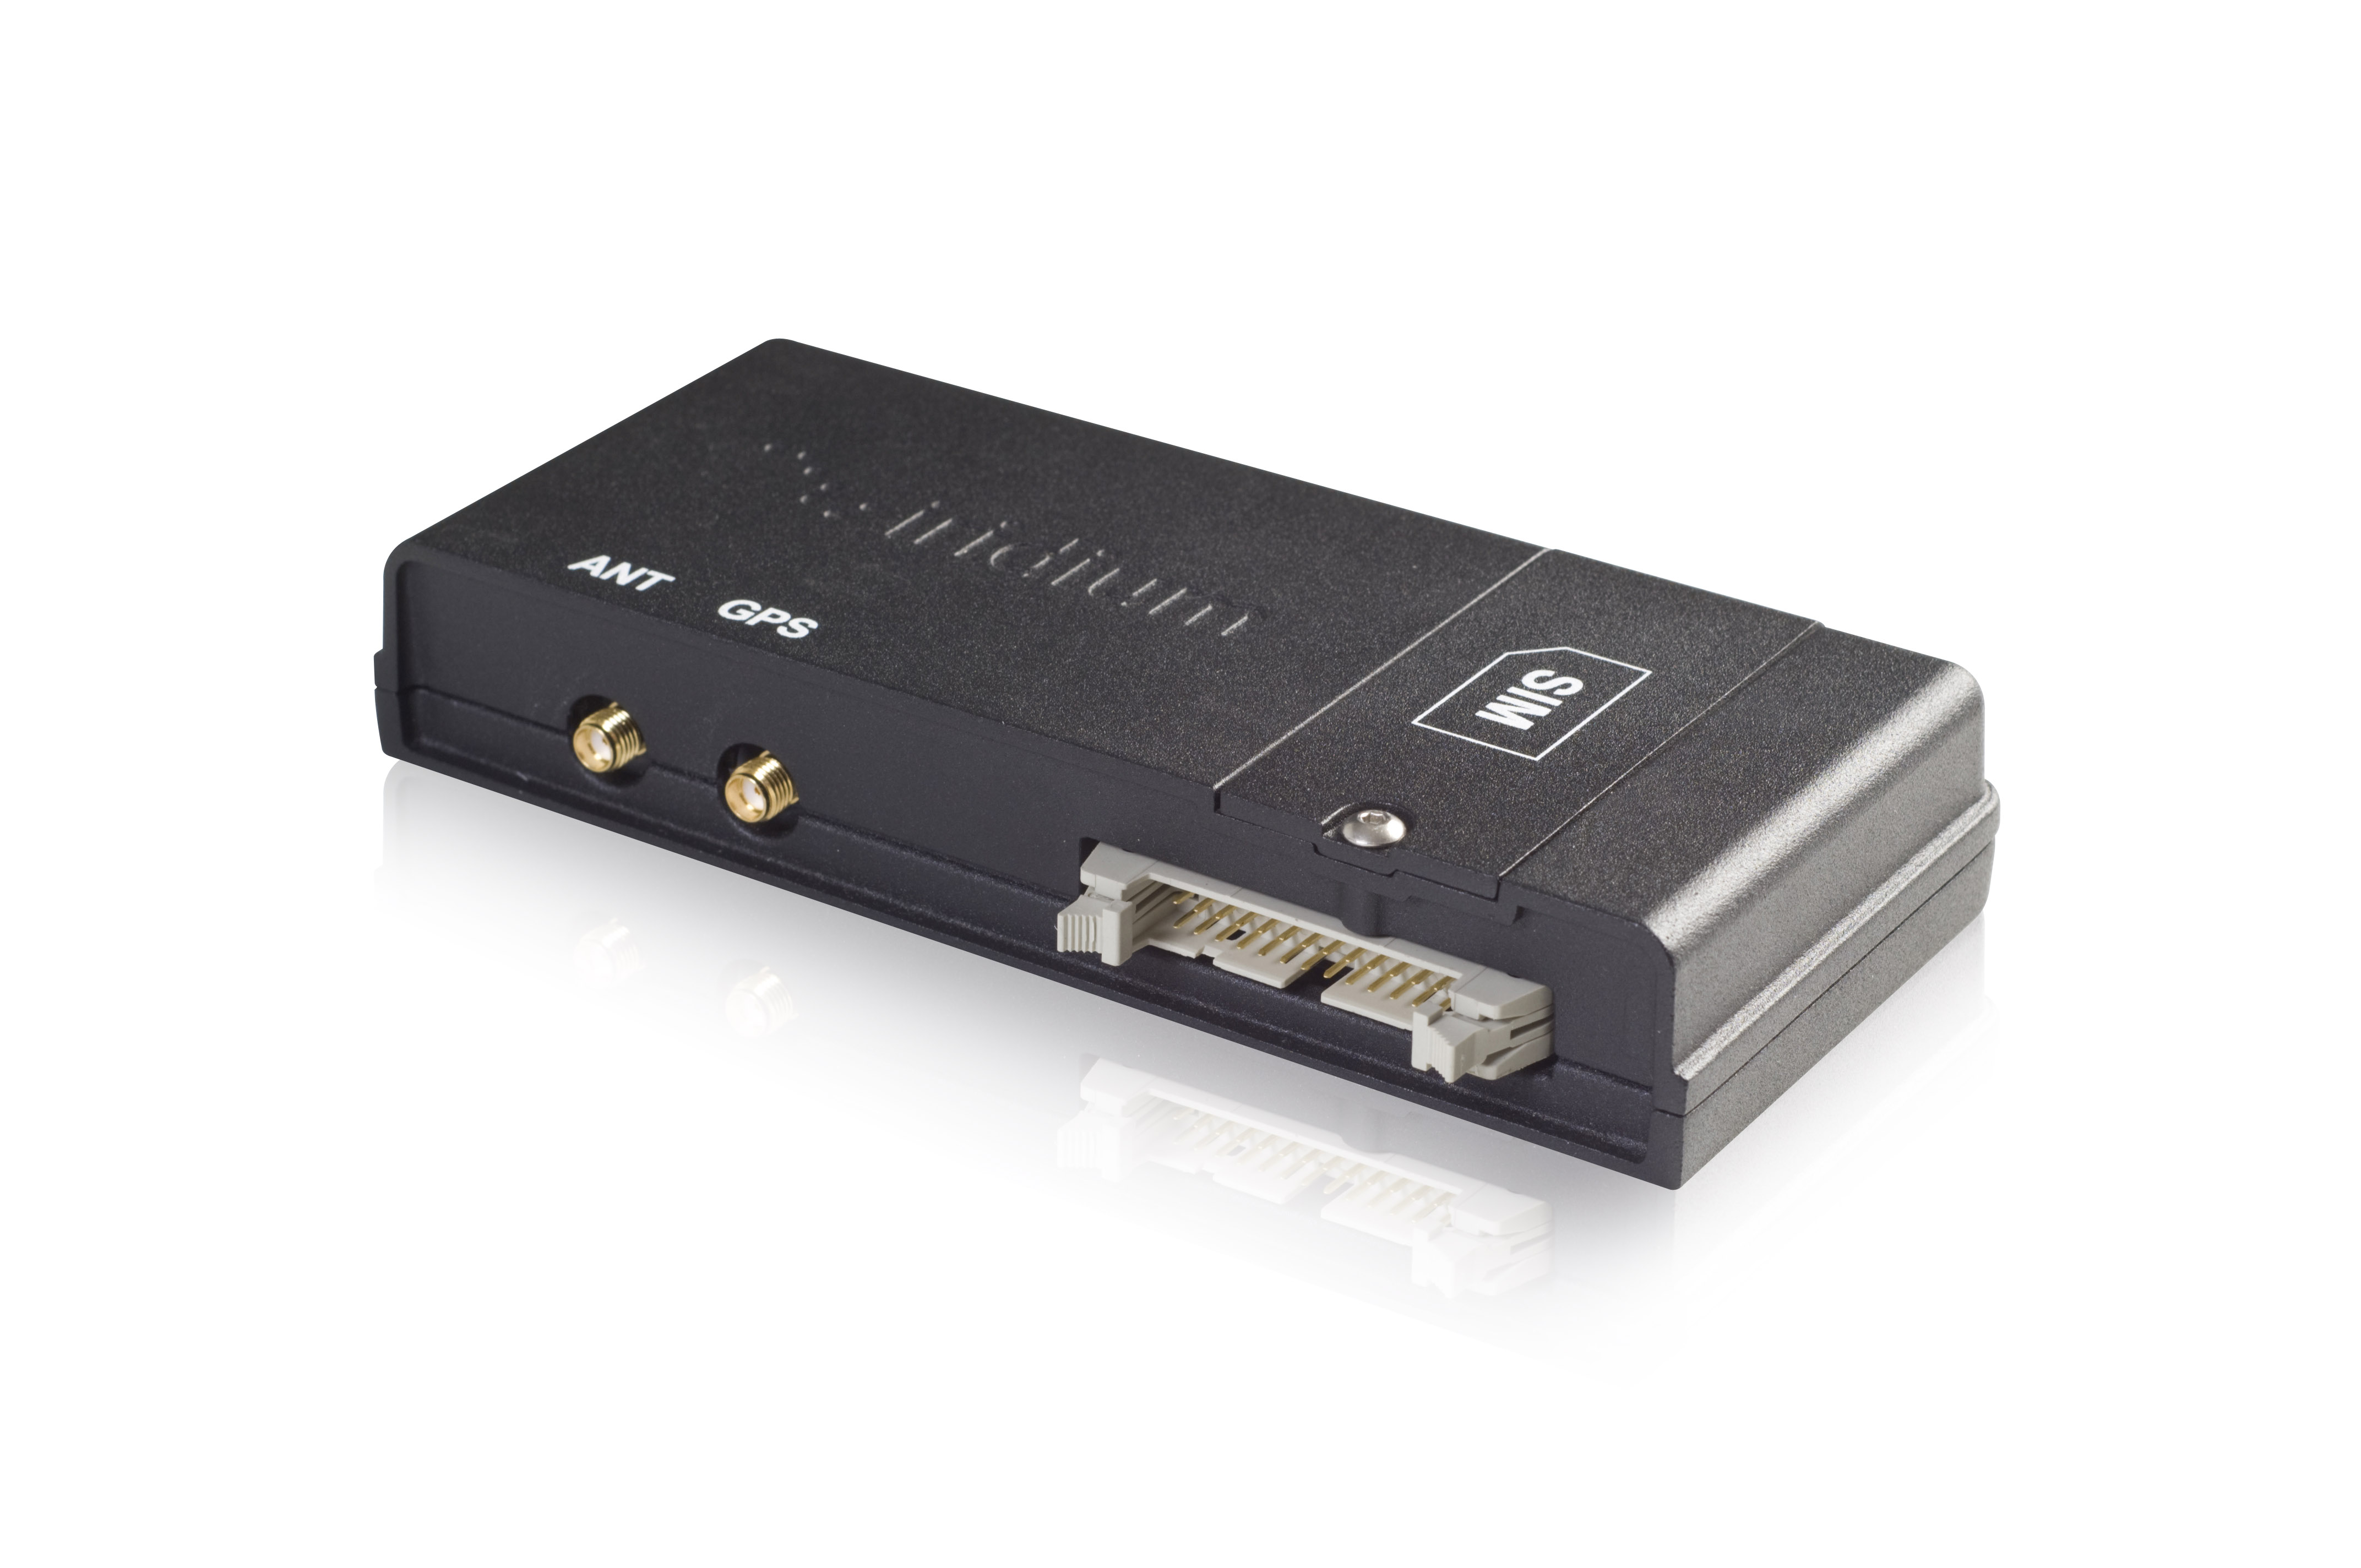
\includegraphics[width = 3cm,height=3cm]{9522B.png}};
			\begin{scope}[x={(image.south east)},y={(image.north west)}]
				\draw[color=black, ultra thin,fill=white] (0.0,0.0) rectangle (0.21,0.16) node[pos=.5] {A};
			\end{scope}
		\end{tikzpicture}
	\end{subfigure}%
	\hfill
	\begin{subfigure}[b]{0.3\textwidth}
		\begin{tikzpicture}
			\node[anchor=south west,inner sep=0] (image) at (0,0) { 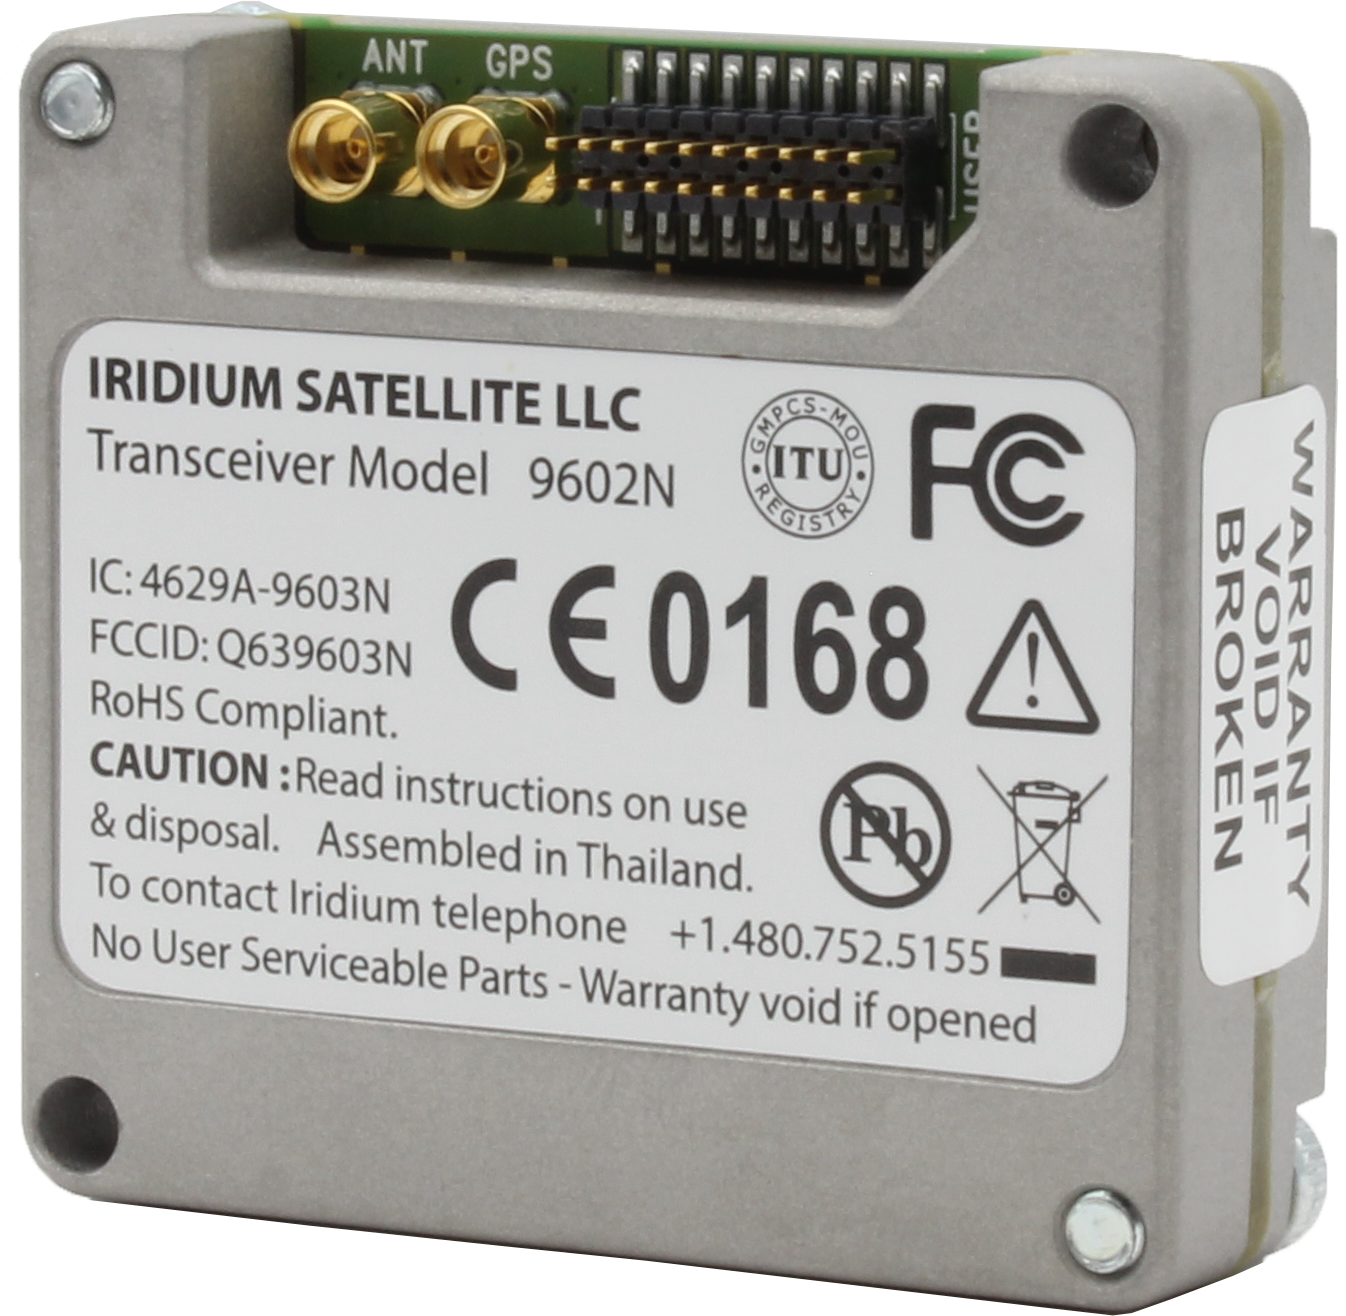
\includegraphics[width = 3cm,height=3cm]{9602.png}};
			\begin{scope}[x={(image.south east)},y={(image.north west)}]
				\draw[color=black, ultra thin,fill=white] (0.0,0.0) rectangle (0.21,0.16) node[pos=.5] {B};
			\end{scope}
		\end{tikzpicture}
	\end{subfigure}%
	\hfill
	\begin{subfigure}[b]{0.3\textwidth}
		\begin{tikzpicture}
			\node[anchor=south west,inner sep=0] (image) at (0,0) { 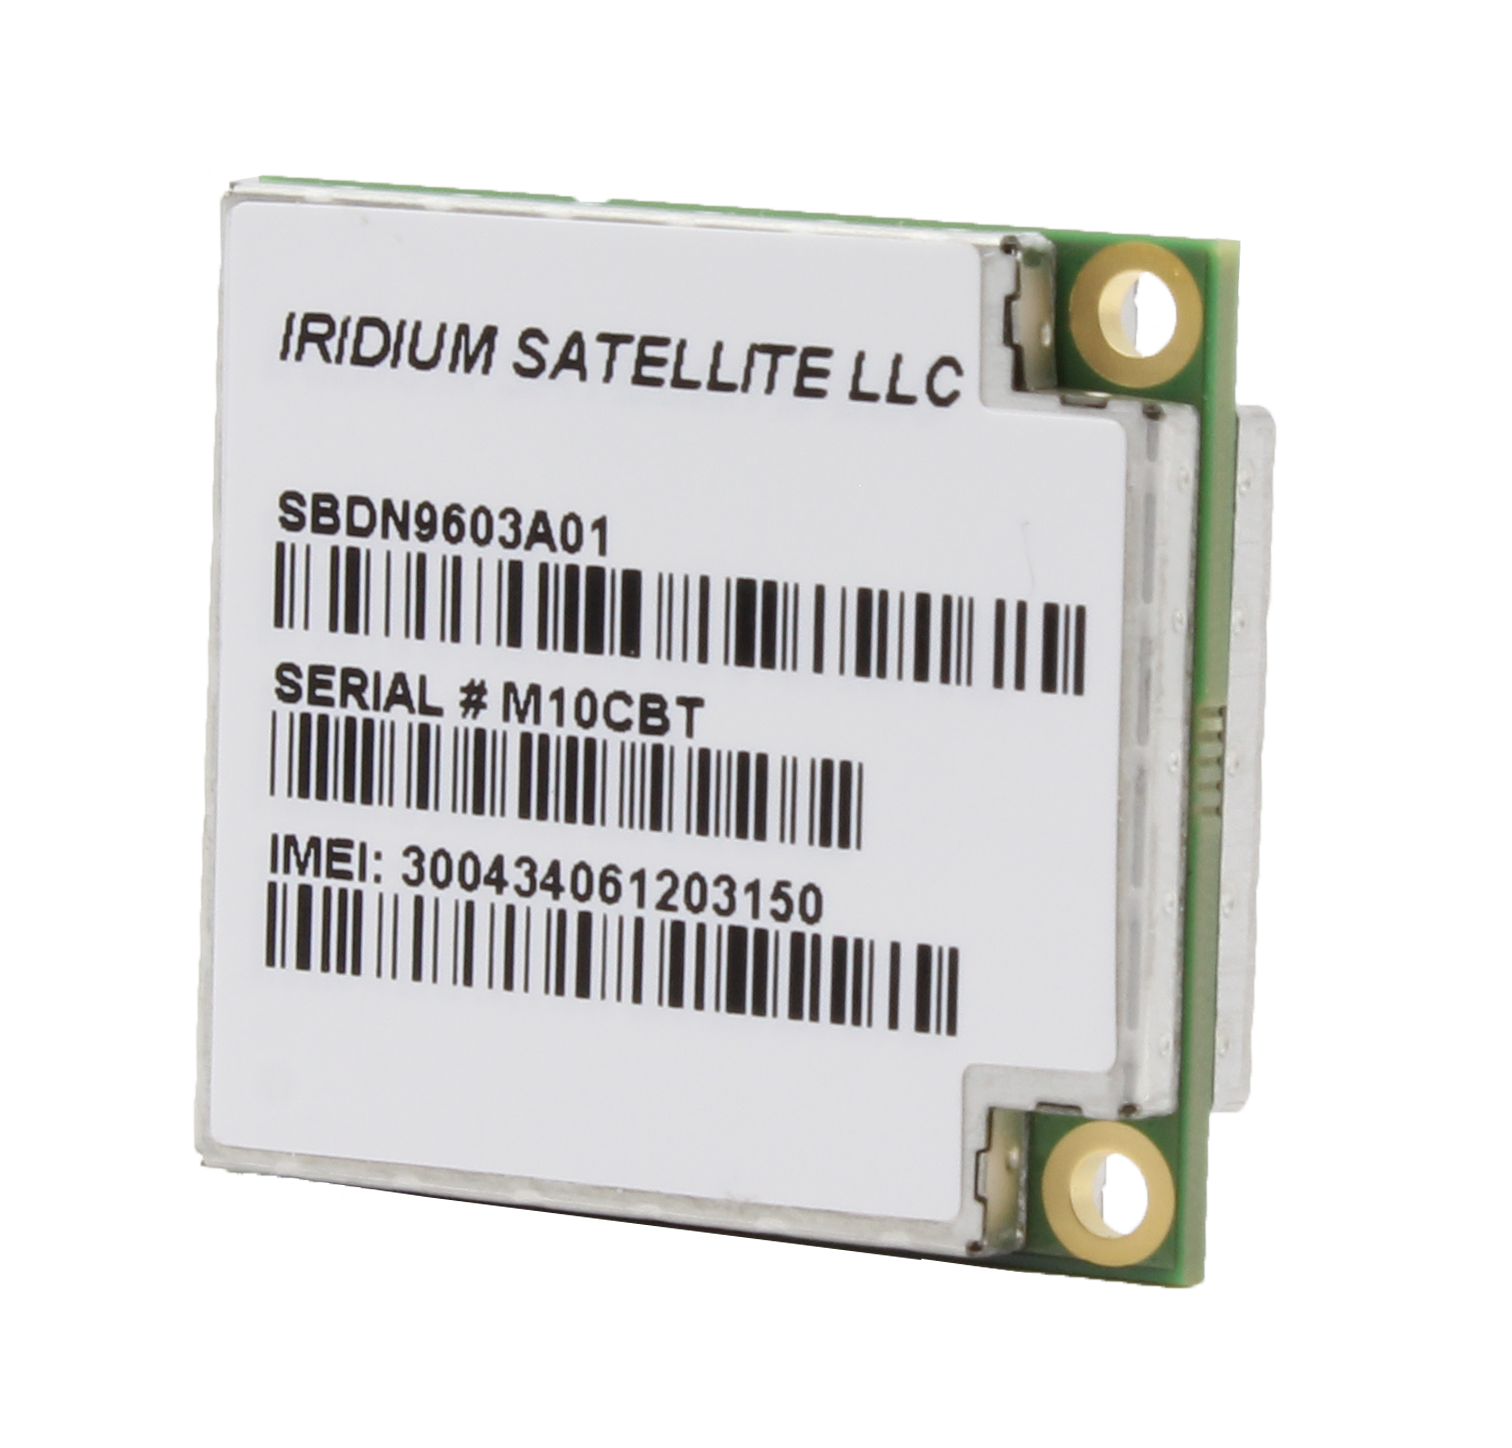
\includegraphics[width = 3cm,height=3cm]{9603.png}};
			\begin{scope}[x={(image.south east)},y={(image.north west)}]
				\draw[color=black, ultra thin,fill=white] (0.0,0.0) rectangle (0.21,0.16) node[pos=.5] {C};
			\end{scope}
		\end{tikzpicture}
	\end{subfigure}%
	\hfill
	\caption{Examples of popular iridium modems selected for remote communications. The 9522B modem (A) (image source: \cite{9522B}), 9602 modem (B) (image source: \cite{9602}) and 9603 modem (C) (image source: \cite{9603})} 
	\label{fig:irid_modem}
\end{figure}

Table \ref{tab:device_transmissionstrategies} shows the satelite network used by each device. All device use Iridium as the primary remote communication method. Other short range wireless systems such as Zigbee \cite{guimaraes2018surface} are alluded to however these systems are only used when the device is close by. Notably, The SIMB buoy details consideration for remote communication using the ARGOS satellite network however, the unreliability of the network resulted in irregular timestamped data \cite{planck2019evolution}. The network service, modem and transmission strategy of each device is shown in table \ref{tab:device_transmissionstrategies}.


\begin{table}[H]
	\centering
	\caption{ The following Iridium modems are compared in their key specifications. devices in the table were suitable for IoT applications based on prevalence in literature and recommendations from the manufacturer. Key parameters include weight, power consumption and transmission latency.Taken from \cite{iridium_product} }
	\label{tab:ir_devices}
	\resizebox{\textwidth}{!}{%
		\begin{tabular}{|l|c|c|c|c|c|}
			\hline
			\textbf{Device Name: } & \textbf{9602} & \textbf{9603} & \textbf{9522B\footnotemark} & \textbf{9523} & \textbf{Edge}\\
			\hline
			Weight (g) & 30 & 11.4 & 420 & 32 & 330 \\
			\hline
			Input Voltage (VDC) & 5 &5 & 4 -32 & 3.2-6 & 9 - 32V\\
			\hline
			Idle Current (mA) & 35 & 34 & 250 & 70 &300\\
			\hline
			Transmit Current (mA)& 140 & 145 &2.5$\times10^3$&500& 300 \\
			\hline
			Recieve Current (mA) & 40 & 39 &2.5$\times10^3$&110 & 300 \\
			\hline
			Packet Latency (s) &  20  &  20 & N/A &45 s& 20s\\
			\hline
			Price &	R2,526.07\footnotemark & 2,526.07\footnotemark & R23,317.40\footnotemark& R13,123.10\footnotemark & R5,638.18\footnotemark\\
			\hline
	\end{tabular}}
\end{table}
\footnotetext[2]{source: \url{https://www.rock7.com/shop-product-detail?productId=49}}
\footnotetext[3]{source: \url{https://www.rock7.com/shop-product-detail?productId=50}}
\footnotetext[4]{source: \url{https://satellitephonestore.com/catalog/sale/details/iridium-9522b-transceiver-496}}
\footnotetext[5]{source: \url{https://www.africasatellite.com/Iridium-9523-Core-Module-p/iridium-9523-core-module.htm}}
\footnotetext[6]{source: \url{https://www.rock7.com/shop-product-detail?productId=56}}

%figure of open-source buoy using the modem
Unanimously, all devices use the Iridium satellite network for remote communication with the Iridium 9602/3 SBD modem being used the most.  This choice is justified for its small form factor, low power and easy interfacing as shown in table \ref{tab:ir_devices} however it suffers greatly from limited bandwidth having a maximum transmission size of 340 bytes. Systems that use these modems for transmission of wave data rely on complex data processing algorithms and therefore do not transmit the raw time series. The only notable exception to this is the wave buoy developed by \textcite{doble2017robust} which continuously transmitted  data from an attitude and heading reference system (AHRS) as well as IMU time series data once every minute. For this purpose, they used the 9522B modem which allowed for continuous transmission using the RUDICS data service. This modem, along with the SBD modem used for the SWIFT Buoy also has a much larger SBD data buffer (1.92KB) However this device draws the most current during idle, transmit and receive states. Additionly this modem is expensive costing R23,317.40 compared to the 9523 (R13,123.10) and the 9602/3 (R2,526.07).  

\subsection{Power Supply}

A robust power supply is critical to support the functionality of a remotely deployed device. A successful power supply can extend the deployment range, duration, processing capabilities and functionality of sensors \cite{kennicutt2016delivering}. Device operation in the Southern Ocean MIZ presents a challenge where the constant freezing/ refreezing of the ocean surface layer prevents long-term infrastructure from being implemented. Hence, a remote device for sea ice monitoring requires a portable power source. Figure \ref{fig:powermoddiag} shows a diagram of a typical power module for a remote sensing device.

\begin{figure}[H]
	\centering
	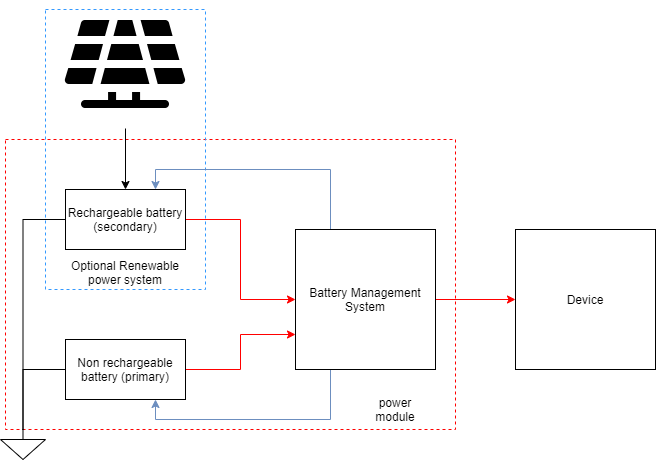
\includegraphics[width = \linewidth]{power module diagram.png}
	\caption{A block diagram of a typical power module for a remote sensing device based off the information from \cite{rabault2019open,doble2017robust,vidal2019xev}. Batteries are used as a primary source of energy which is connected to a battery management system to control and regulate the power supply to the device. optionally, solar panels are implemented with a rechargeable battery as a secondary power supply. Shown in the figure: flow of power (red), control lines (blue) and ground (black).}
	\label{fig:powermoddiag}
\end{figure}

Batteries such as lithium-ion are commonly used as sources of power for in situ devices. Batteries typically fall into one of two categories:
\begin{enumerate}
	\item Primary: Cells that cannot be recharged once they are depleted. These batteries have a high energy density and can store charge for long periods.\cite{besenhard2008handbook}
	\item Secondary: Cells that can be recharged. These cells are more cost effective with longer usage cycles \cite{besenhard2008handbook}.
\end{enumerate}

Lithium  Ion and Alkaline batteries are examples of primary cells that have commonly been used as they provide a cost effective solution due to their high energy density and long-term consistent life cycles \cite{zareer2018review}.  Secondary cells such as lead-acid, nickel-metal hydride and lithium polymer are commonly used coupled with a secondary charging circuit such as a solar panel \cite{manimekalai2013overview} to provide a more constant source of power. While batteries are cost effective solutions, the climate of the Southern ocean can affect the battery performance. Freezing air temperatures can reduce the capacity of a standard lithium cell by up to 50\% for temperatures below $-10^\circ C$ \cite{doble2017robust,ZHANG2003137}. Additionally, frozen batteries/ ice formation on batteries can stop them from working \cite{doble2017robust,manimekalai2013overview}.A solution to compensate for this reduction is to use rechargeable batteries coupled with a renewable power sources such as solar \cite{doble2017robust,rabault2019open}, wind and geothermal energy \cite{manimekalai2013overview}.Solar photovotaic (PV) cells is the fastest growing renewable energy source with the highest energy density \cite{jordehi2016parameter}. PVs have numerous advantages such as low maintenance and operational costs, wide temperature operations and long life-cycles \cite{jordehi2016parameter} which makes them ideal for long term operation in remote environments. However, the power output of PV cells are significantly affected by weather conditions \cite{sharma2015solar}. Therefore, areas with poor sunlight coverage will not benefit from solar panels. Additionally, power generation from solar panels is inconsistent and requires an additional storage bank capable of frequent charging and discharging. Wind energy can provide a viable alternative to solar energy. \textcite{vichi2019effects} show that the Southern Ocean hosts strong, consistent winds. However, the design and implementations have not been discussed in any of the literature. Therefore this options is provided as an area for future research. Finally, a critical component of the power system is a battery management system. This allows the power supply to opperate under safe conditions while meeting performance requiremnt \cite{vidal2019xev}. This module includes power monitoring, power control and energy cycle optimization. Table \ref{tab:device_power_source} below shows the power sources used by each device and the strategy used to manage it.
\begin{table}[H]
	\centering
	
	\caption{A comparison of power supply strategies of the different devices  showing the the power source, topology of the power supply module as well as the voltage supplied at the output of the module. Information that was unavailable at the time of research has been labeled as "Not reported"}
	\label{tab:device_power_source}
	
	\setlength{\extrarowheight}{5pt}%
	\resizebox{\textwidth}{!}{%
		\begin{tabular}{|>{\centering}m{3cm}|>{\raggedright\arraybackslash}m{4cm}|>{\raggedright\arraybackslash}m{4cm}|>{\raggedright\arraybackslash}m{4cm}|>{\raggedright\arraybackslash}m{4cm}|>{\centering\arraybackslash}m{3cm}|}
			\hline
			\textbf{Device Name} & \textbf{Primary Power Source} & \textbf{Secondary Power Source} & \textbf{Battery Management System} & \textbf{Output Regulation Strategy} & \textbf{Output Voltage} \\
			\hline
			WIIB & Lithium Iron Phosphate (LiFePO4) battery & None & ATMega328P for Power control & Boost Converter & 5V \\
			\hline
			WIIOS & Alkaline battery & None & Integrated into firmware & 8-cell series configuration, no regulator & 12V \\
			\hline
			NDWB & Alkaline battery & Solar panel and lead-acid battery & Not Reported & Not Reported & 12V \\
			\hline
			SKIB & Lithium thionyl chloride (LiSOCl2) battery & None & Not Reported & Not Reported & 3.6V \\
			\hline
			SWIFT & Alkaline or Lithium  battery& None & Not Reported & Not Reported & 14V \\
			\hline
			SIMB & Alkaline battery & None & Not Reported & LMZ12003 Step Down Converter (5V, 3.3V)\par MIC29201-12W Low dropout regulator (12V) & 3.3V \par 5V \par 12V\\
			\hline
			Polar ISVP & LiSOCl2 battery & None & Not Reported & Not Reported & 12V \\
			\hline
			Trident & Lithium cell battery & None & integrated into firmware & Low dropout regulator & 5V\\
			\hline
	\end{tabular}}
\end{table}
\footnotetext{Information available online at \url{https://github.com/jerabaul29/LoggerWavesInIce_InSituWithIridium/blob/master/ElectronicsList/list.md}}

Table \ref{tab:device_power_source} shows the power supply strategies of each device. All systems use primary batteries as a source of power with the most common choice being alkaline or lithium-based batteries. However, \textcite{doble2017robust} is the only exception where a secondary power source was adde consisting of a solar panel and lead-acid batteries. Systems deployed in the Arctic Marginal Ice Zone have been designed with a recharging system such as a solar panel in the case of WII Buoy and NDWB, however, most long-range deployment buoys have opted for non-rechargeable systems composed of Lithium Thionyl Chloride (LISOCL2) or Alkaline batteries. In the case of the high-power buoys (SIMB, WIIOS, NDWB, Polar ISVP) an array of 3.3V -3.7V cells is connected to provide a nominal voltage in series with a regulator to provide a stable output. The strategy for each system is to pack as many batteries in as possible to satisfy the long-term energy requirements \cite{doble2017robust,rabault2019open}. Finally, few devices have reported their battery management strategies. \textcite{rabault2019open} used an ATMega328P microcontroller as a power controller for their device which monitored the status of the battery. \textcite{trident} and \textcite{kohout2015device} however integrated power control into their main firmware allowing for them to control and monitor their power source off a single processor.

\subsection{Polar Performance}

This section outlines the deployment of the systems in the Arctic/Antarctic marginal ice zones and compares the survivability and performance of each system. The focus of this section will be predominantly on devices deployed in the marginal ice zone. Table \ref{tab:device_components} shows the significant deployment locations in the Arctic and Antarctic sea ice zones as well as the deployment objectives of each device. 

\begin{table}[H]
	\centering
	\caption{ comparison between the functionality and purpose of the buoy showing the critical measurements as well as the significant deployment locations either in the polar ice zones or in a location critical to the validation of the device.}
	\label{tab:device_deployment}
	\setlength{\extrarowheight}{5pt}
	\resizebox{\textwidth}{!}{
		\begin{tabular}{|l| >{\raggedright\arraybackslash}m{5cm}|>{\raggedright\arraybackslash}m{5.4cm}|>{\raggedright\arraybackslash}m{5cm}|}
			\hline
			\textbf{Device name} & \textbf{Deployment objectives} & \textbf{Antarctica Deployments} & \textbf{Arctic deployments}\\
			\hline
			\multirow{3}{*}{WIIB} & Wave energy attenuation &  Ross Sea landfast ice \cite{rabault2020development} &  Templefjord (Svalbard) landfast ice \cite{rabault2019open} \\
			& Significant wave height &  & Northeast Barents sea \cite{rabault2019open}\\
			& Data quality && \\
			\hline
			\multirow{5}{5cm}{WIIOS} &Ice drift&Ross sea marginal ice zone \cite{kohout_smith_roach_williams_montiel_williams_2020}&\multirow{5}{*}{-}\\ 
			& Waves in ice & Ross Sea packed ice zone \cite{kohout2015device} & \\ 
			& Ambient temperature & Weddel Sea marginal ice zone \cite{albarello2020drift}& \\
			& Atmospheric pressure && \\
			\hline
			\multirow{4}{*}{NDWB} & Ice drift  & \multirow{4}{*}{ - } & \multirow{4}{5cm}{Beaufort sea \cite{doble2017robust}} \\
			& Wave induced ice breaking &&\\
			& Ambient temperature &&\\
			& Atmospheric pressure &&\\
			\hline
			\multirow{2}{*}{SKIB} & Ice drift &\multirow{2}{*}{-} & North Atlantic ocean (France) \cite{guimaraes2018surface}\\
			& Surface waves &&\\
			\hline
			\multirow{6}{*}{SWIFT} & Surface images & Ross Sea \cite{ackley_2020_seaice} & Chukchi sea \cite{hosekova2020Attenuation} \\
			& Ocean waves & Weddel sea \cite{DeSanti2018OceanWave} &  Beaufort sea \cite{lund2018Arctic} \\
			& Turbulence profiles &&\\
			& Ocean current profiles &&\\
			& Conductivity && \\
			&Wind speed and direction && \\
			\hline
			\multirow{6}{*}{SIMB} & Surface and bottom ice position &Weddel sea \cite{hoppmann2015fmot} & Beaufort sea marginal ice zone \cite{PLANCK2019102792} \\
			& Snow depth& & \\
			& Atmospheric pressure&& \\
			& Ambient temperature &&\\
			& Vertical temperature profile& & \\
			& GPS Location&&\\
			\hline
			\multirow{3}{*}{Polar ISVP} & Sea ice drift & \multirow{3}{5.4cm}{Weddel Sea marginal ice zone \cite{deVos2021evaluating}} & \multirow{3}{5cm}{Western Arctic Ocean \cite{lei2020comparisons}}\\
			& Ambient temperature & &\\
			& Atmospheric pressure &&\\
			\hline
			\multirow{3}{*}{Trident} & Sea ice drift & \multirow{3}{5.4cm}{Weddel sea \cite{alberello2019drift}}
			& \multirow{3}{*}{-}\\
			& Ambient temperature & &\\
			& Battery voltage &&\\
			\hline
		\end{tabular}
	}
\end{table}

\textcite{kohout2015device} deployed five Wave in Ice Observational Systems (WIIOS) in the East Antarctic marginal ice zone during the Sea Ice Physics and Ecosystem Experiment (SIPEX) mission\footnote{1st deployment occured September 2012 \cite{kohout2015device}} with the goal of capturing wave in ice events with measurement goals shown in table \ref{tab:device_deployment}. Three devices were deployed by helicopters on ice floes while two devices were deployed via the ships crane. \textcite{kohout2015device}
note that deployment via crane was successful in spite of 7 m swell and 25 $m.s^{-1}$ winds. The device was fitted inside a Pelican box with a sealed membrane surrounded by a tyre for protection and flotation in case of melting \cite{kohout2015device}. Consequently, this places the buoy directly on the surface of the floe rendering it susceptible to snow build up and flooding as mentioned in the previous sections.  After deployment, the crew received 600 samples of data over 39 days in total. However, the first device failed 20 hours after deployment coinciding with the first large wave event captured the buoys \cite{kohout2015device}. The second large wave event resulted in the failure of two more systems just 9 days after deployment \cite{kohout2015device}. The fourth buoy lasted for 17.5 days. The final buoy survived the longest at 39 days. As a result only one device lasted for the expected time with the majority of data captured during calm events.

\begin{figure}[H]
	\centering
	\begin{subfigure}[b]{0.45\textwidth}
		\begin{tikzpicture}
			\node[anchor=south west,inner sep=0] (image) at (0,0) {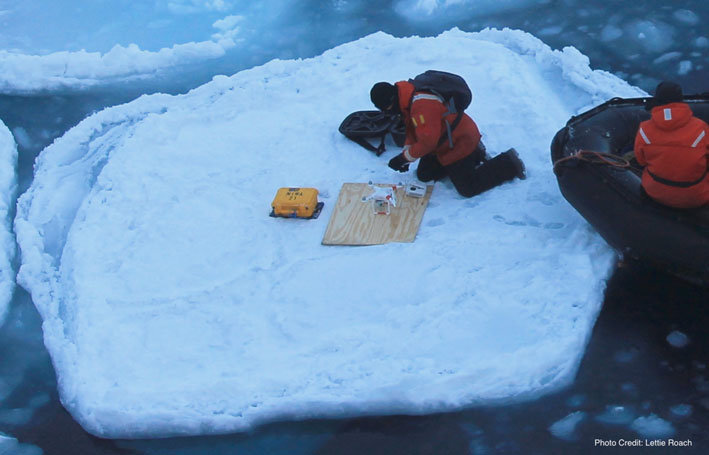
\includegraphics[width = 6cm,height=8cm]{WIIOS.png}};
			\begin{scope}[x={(image.south east)},y={(image.north west)}]
				\draw[color=black, ultra thin,fill=white] (0.0,0.0) rectangle (0.21,0.16) node[pos=.5] {A};
			\end{scope}
		\end{tikzpicture}
	\end{subfigure}%
	\hfill
	\begin{subfigure}[b]{0.45\textwidth}
		\begin{tikzpicture}
			\node[anchor=south west,inner sep=0] (image) at (0,0) { \includegraphics[width = 6cm,height=8cm]{Basket.jpg}};
			\begin{scope}[x={(image.south east)},y={(image.north west)}]
				\draw[color=black, ultra thin,fill=white] (0.0,0.0) rectangle (0.21,0.16) node[pos=.5] {B};
			\end{scope}
		\end{tikzpicture}    
	\end{subfigure}
	\caption{ Examples of different deployment protocols for ice tethered devices. In regions of consildated ice in favourable conditions, manned crews will step foot on the ice to deploy the device (A) (image source: \cite{kohout2020observation}), in unfavourable conditions, devices may deployed from a basket attached to a crane (B). A manned crew will lower the buoy on a suitable ice floe from the safety of the basket (image source: N. Taylor) }
	\label{fig:deploy}
\end{figure}
Two additional WIIOS buoys were deployed by \textcite{alberello2019drift} during the winter\footnote{first deployment occured in July 2017 \cite{alberello2019drift}}. Here, the buoys lasted significantly shorter than the previous deployment. The first system survived for 8 days while the second system survived for 3 weeks in spite of measures taken to place the device in power saving mode \cite{alberello2019drift}. This was achieved by lowering the sample period from to 2 hours. Consequently, the lower temporal resolution resulted in a significantly reduced accuracy of the ice deformation calculations \cite{alberello2019drift}. However, despite this low resolution, by operating at a temporal scale of 3 hours or less \cite{alberello2019drift}, one can effectively and accurately capture ice drift speed as well as the oscillations surrounding the movement. Additionally, \textcite{vichi2019effects} and \cite{albarello2020drift} discuss the deployment of two Wave in Ice Observation Systems similar to the ones by \cite{kohout2015device}. 2 devices were deployed on two separate ice floes 3 m in diameter and 100 km from the ice edge \cite{albarello2020drift}. One system survived for 8 days and 18 hours while sampling every 15 minutes before transmission ended \cite{albarello2020drift}. The second buoy however, survived for 6 days sampling every 15 minutes until it switched to power saving mode surviving for a total time frame of 3 weeks. \textcite{vichi2019effects} deployed a second pair of WIIOS buoys in a similar method to \cite{alberello2019drift} however, the first buoy stopped responding after 3 days while the second buoy survived for only 16 days \cite{vichi2019effects}. While the buoys survival is largely attributed to power optimisation, the lifespan could be influenced by the selection of the ice floe. Ice floe size and proximity to the ice edge affect the exposure of the floe to open-ocean processes and storms \cite{vichi2019effects}. This could result in failure due to ice mechanics which is discussed in section \ref{ch2:sec3_failiure}. \par 

\textcite{rabault2019open} deployed the waves in ice buoy (WIIB) WIIB on land-fast ice in the Ross sea \cite{rabault2020development} to test the device's performance in the Antarctic. In a similar fashion to the WIIOS buoy, the device was placed in a pelican case and attached to a flotation device, however, expected survival time for this device was significantly lower compared to the WIIOS devices: a maximum of 8 days \cite{rabault2019open} of continuous operation. The buoys by \textcite{kohout2015device} were designed to be expendable \cite{alberello2019drift} whereas the buoys by \textcite{rabault2019open} were designed to be retrievable. Additionally, the WIIB devices were deployed in the summer\footnote{First deployment date: December 2019 \cite{rabault2019open}}. Two devices were deployed in proximity however an ice break event resulted in the separation of the devices. The devices survived for 2.5 weeks \cite{rabault2019open} which \textcite{rabault2019open} attribute the failure to the devices having been crushed by ice and wave activity. Despite this, the devices were able to record significant wave events and maintain a fully charged battery throughout the deployment which \textcite{rabault2019open} attributes to the solar panel. 

\par \textcite{doble2017robust} alluded to a series of environmental considerations when designing the NDWB systems. One such consideration is the frosting over/ rimming of the device due to freezing ocean spray. Additionally, auxiliary power sources (i.e. solar panels) would need to account for long periods of no cloud cover \cite{doble2017robust}. Since the buoys were deployed by a manned crew, the design also had to account for ease of handling by the crew and not be too heavy \cite{doble2017robust}. The mechanical enclosure consisted of a float and a keel with the electronics contained above the surface in a dome. Twenty buoys were deployed in the Arctic marginal ice zone with each device anchored by drilling a hole in the ice and placing the keel inside. nineteen buoys survived the deployment with one system failing to boot. The buoys survived for extremely long periods with twelve systems surviving for two hundred days off a single alkaline battery pack \cite{doble2017robust}. A significantly longer period than both the WIIOS and WIIB systems. Seven systems ran for 70 days on alkaline batteries before switching over to  the solar powered lead-acid batteries. During this period, devices transmitted continuously over the Iridium network and were able to interpolate sea ice phases (see Section \ref{sec:ch1.section1}) from the tilt of the buoy \cite{doble2017robust}.

\subsubsection{Reasons for Failure}
\label{ch2:sec3_failiure}

Eventually, the systems by \textcite{doble2017robust} lost transmission 300 days after their deployment. This can be attributed to the depletion of the alkaline battery packs. The solar powered lead acid battery voltage eventually dropped below the alkaline battery voltage due to the lack of consistent solar coverage \cite{doble2017robust}. Additionally, sub zero temperatures have a tendency to reduce battery capacities by up to 50\% \cite{doble2017robust} however, \textcite{doble2017robust} found this estimate to be over conservative. Systems by \textcite{kohout2015device} and \textcite{doble2017robust} encountered similar failures with devices eventually depleting the on-board batteries. Additionally, \cite{alberello2019drift} attribute failure of the first WIIOS system to the battery being depleted.\par 

Additional sources of failure experienced by \textcite{doble2017robust} include ice convergence. The systems were subject to ice-mechanics and as a result, ended up crushed by the floes due to rafting or buried under ice \textcite{doble2017robust}. These failures were identified when more than one system suddenly went offline. Devices also experienced freeze-over or were buried under snow which resulted in the devices going offline for temporary periods \cite{doble2017robust}. Additional evidence of rafting and ridging was captured by webcams on the buoy shortly before transmission ended \cite{doble2017robust}. Buoys that survived the spring melt refroze during the gradual refreezing of the ice. During the second cycle, none of the buoys rebooted when the ice melted in the spring \cite{doble2017robust}. Finally, the buoys developed by \textcite{kohout2015device} and \textcite{rabault2017measurements} sit in close proximity to the ice floes. As discussed previously, during the winter cycles, snow accumulates on the surface that can reach up to 1m in height. This snow formation can result in flooding where the floe becomes submerged. Prolonged burying under snow may have resulted in the device freezing over thereby losing contact while prolonged contact with the seawater may have resulted in the buoys failing on several occasions (\cite{kohout2015device,vichi2019effects,albarello2020drift,rabault2019open})\par 

\begin{figure}[H]
	\centering
	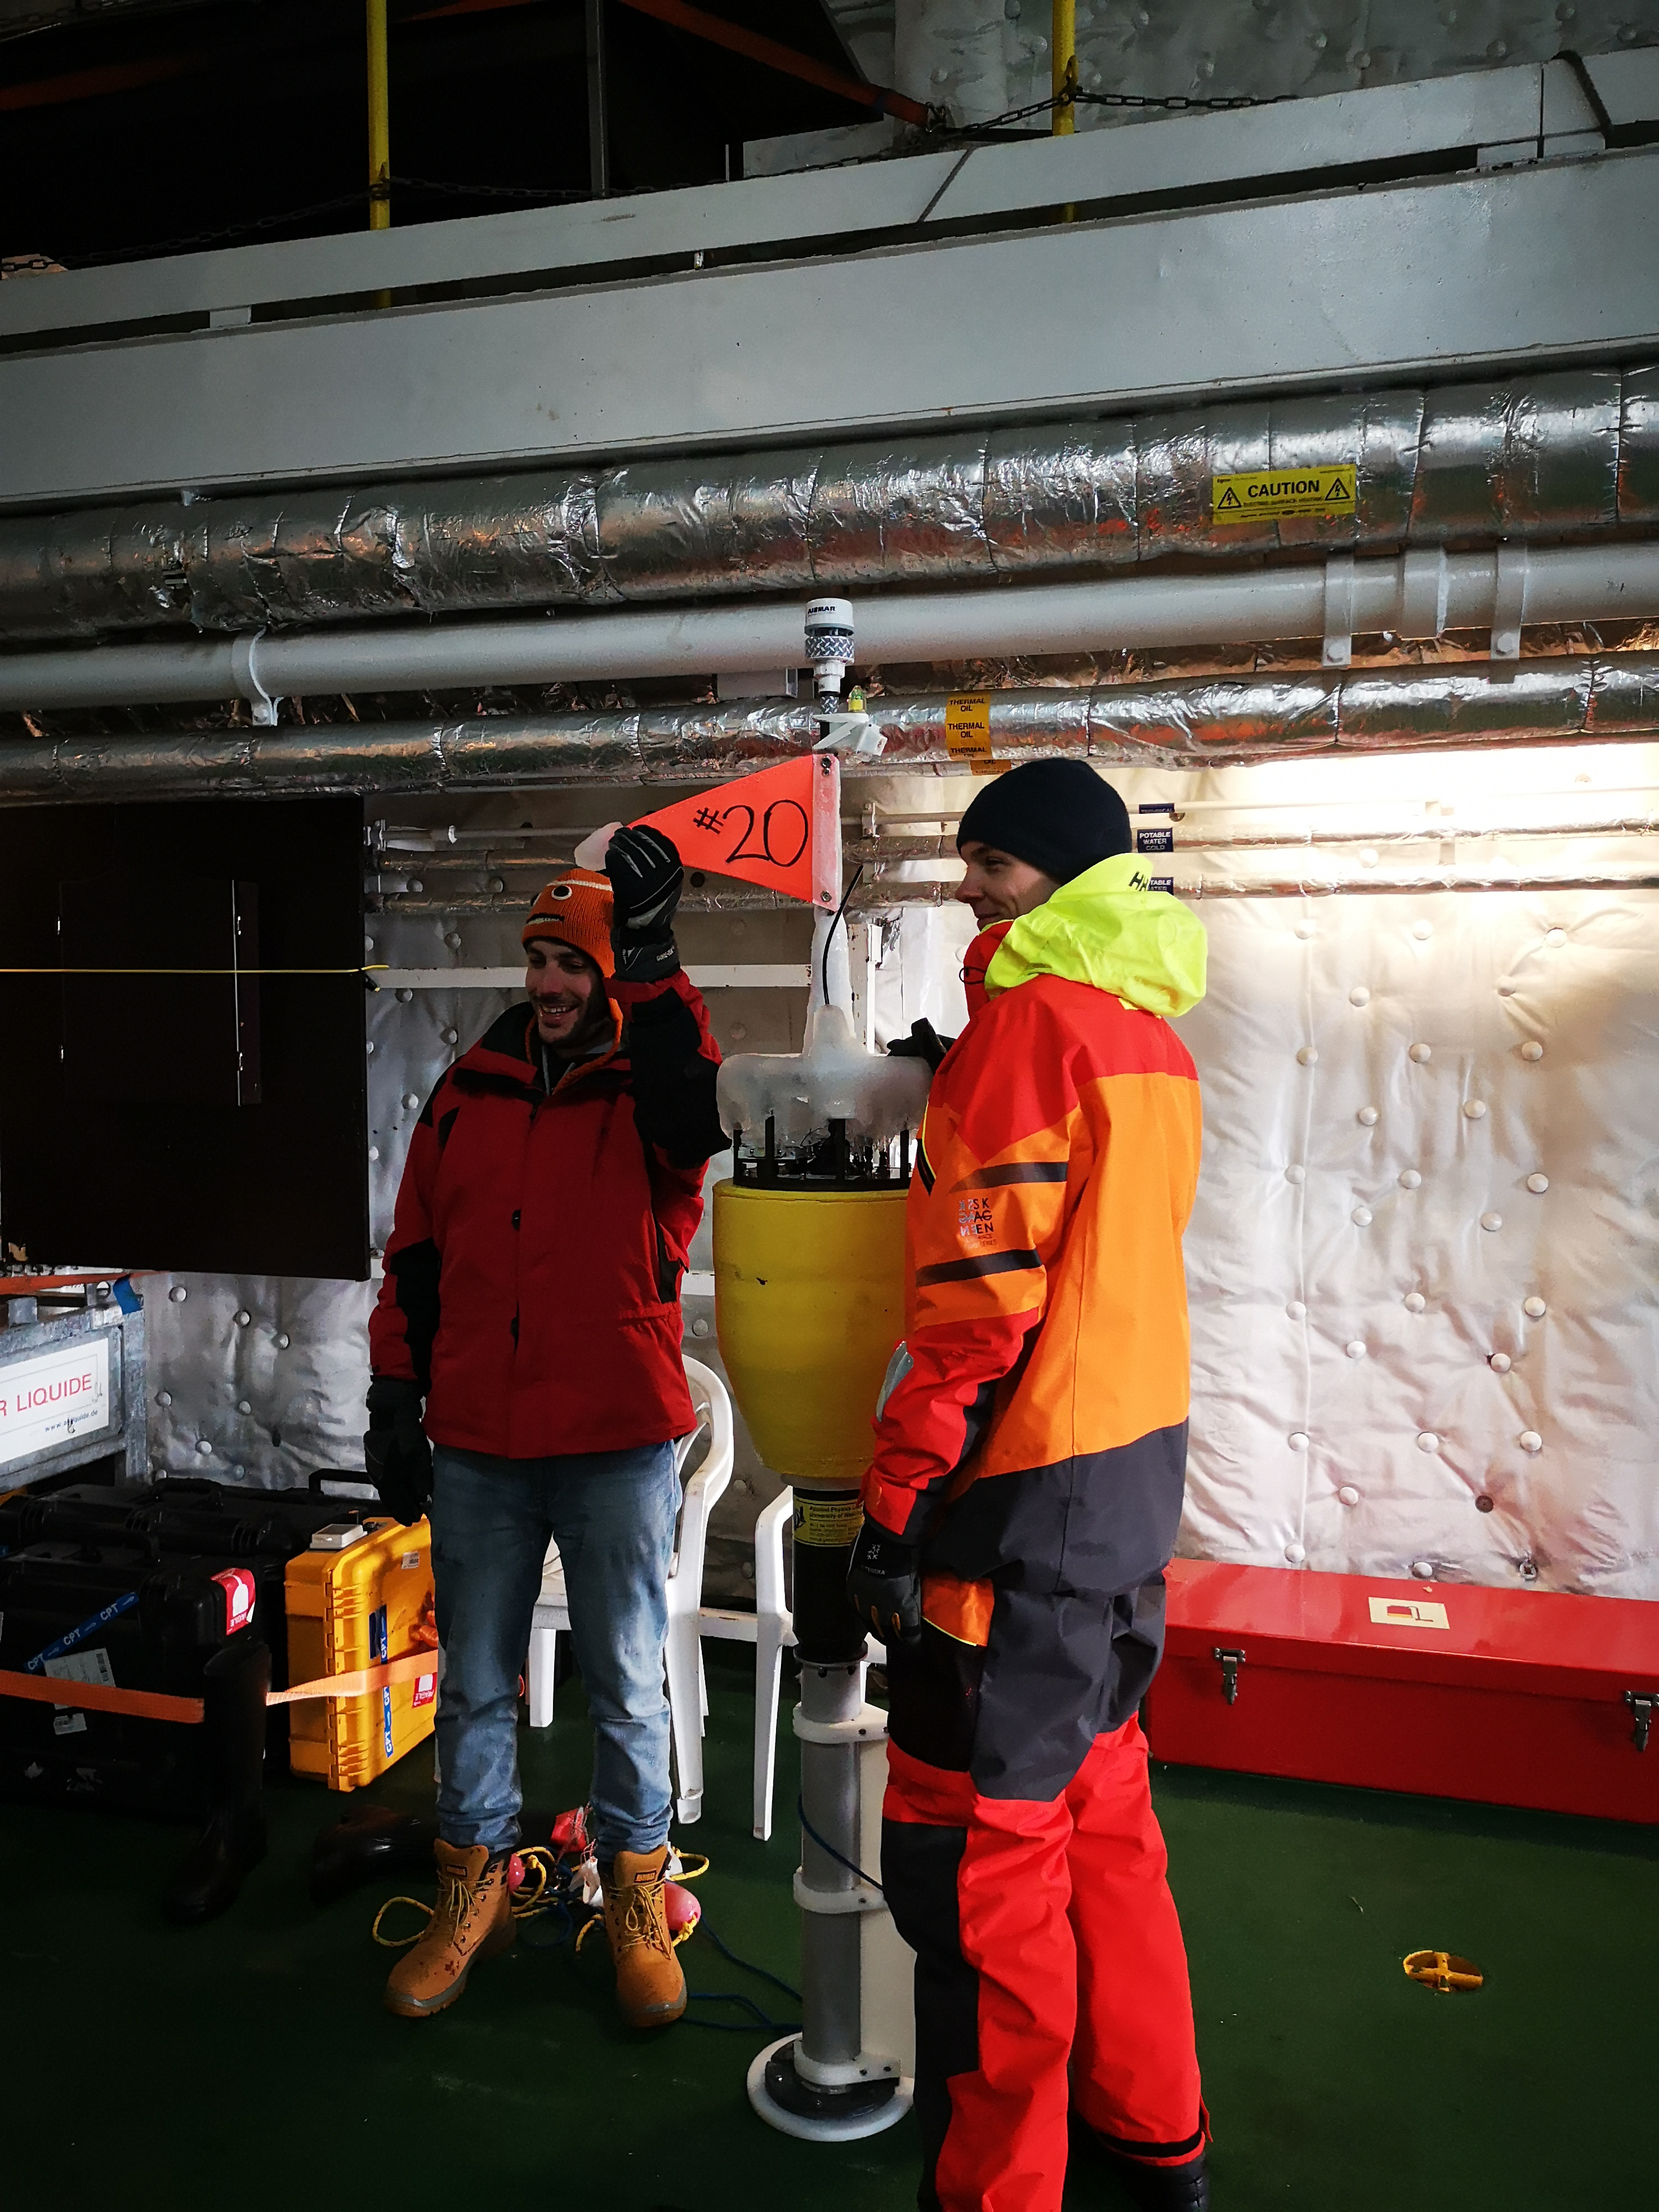
\includegraphics[width = 7cm]{swift_fail.jpg}
	\caption{During the 2019 SCALE winter expedition, a SWIFT device was retrieved early due to lost communication with the host. This failure was attributed to a build up of ice along the the rim from ocean spray. Photo taken by author.}
	\label{fig:swift_fail}
\end{figure}

Finally, \textcite{vichi2019effects} discuss the findings surrounding the failure of the first WIIOS system. \textcite{vichi2019effects} observed a major cyclonic event. The cyclone formed on  2 July 2017 and achieved lysis on 5 July 2017 which coincided with the buoy deployment. Following the event, four more cyclonic events were recorded with three explosive cyclones \cite{vichi2019effects} characterising a change of pressure over 24 hours. During this time, \textcite{vichi2019effects} observed winds speeds of up to $33$ $m/s^{-1}$ while noting that the air temperatures had increased to values "close to melting" \cite{vichi2019effects}. Additional observations found an increase in significant wave height in the activity. These conditions indicate deformation \cite{vichi2019effects} which may have subjected the buoys to forces experienced by \cite{doble2017robust} during their arctic deployment which were verified against the temperature and pressure readings of the second WIIOS during the cyclonic event. The buoys were deployed close to the ice edge exposed to greater open ocean processes and cyclonic activities than other semi-consolidated and consolidated regions \cite{vichi2019effects}. As a result, air advection, storms and large wave movement delay the consolidation of sea ice considerably \cite{vichi2019effects}. Hence, the ice floes were more likely to experience rafting, ridging \cite{icedefinition1992}, extended flooding, and freezing over which may have caused the failures of the WIIOS buoys.
\newpage
\section{Subsystem Overview}

This section focuses on the subsystem analysis and component selection for each system. As stated previously, each buoy was created with a unique objective shown in table \ref{tab:device_deployment}. These objectives have influenced the sensor selection, topology and layout of the overall subsystems. In addition, the device designs choices have been influenced objectives for developing new in situ technologies by \textcite{kennicutt2016delivering} as the device developers have factored in power consumption \cite{kohout2015device}, ease of use and deployment \cite{rabault2019open}, long-term operation \cite{doble2017robust},cost \cite{planck2019evolution,rabault2019open} and availability of infrastructure \cite{doble2017robust} over and above functionality. For example WIIB was developed using open-source hardware \cite{rabault2019open} in order to increase access to readily available technology while WIIOS was developed using off-the-shelf components \cite{kohout2015device} to create a cost effective device. From table \ref{tab:device_deployment} we saw that the principle measurements of each device share the following measurement objectives:

\begin{enumerate}
	\item Ice drift
	\item Wave data/Wave in Ice data
	\item Ambient temperature
	\item Atmospheric pressure 
\end{enumerate}

The following sections discuss how these objectives have influenced sensor selection for each of these measurements as well as the hardware, and software strategies implemented to achieve these objectives.

\subsection{Processing capabilities}

The processing capabilities of each device facilitate the functionality of each buoy. A strong processor allows for the implementation of in-situ data processing and wave analysis algorithms \cite{kohout2015device,rabault2019open}. Additionally, due to the bandwidth constraints mentioned in section \ref{ch2:sec_remote}, some devices require data compression algorithms to allow the data to fit in the transmission buffers. The functionality of these devices has been made possible through the use of microprocessors.

\begin{figure}[H]
	\centering
	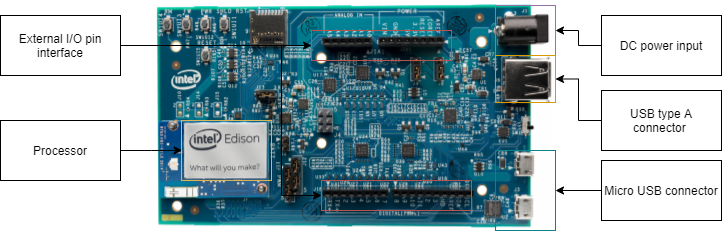
\includegraphics[width = 0.9\textwidth]{edison.png}
	\caption{Diagram of a typical microprocessor (yellow) on a development board. This device is an Intel Edison which was used as the main processor \textcite{kohout2015device} for the WIIOS. The development board allow for fast prototyping and integration into projects. The processor interface with external peripherals through physical input/output pins (Red) and contains standard serial communication ports such as USB (orange), micro USB (teal) and a connector for external voltage (purple). Image source: \cite{edison} }
\end{figure}

These are programmable integrated circuits that contain processing elements \cite{subham2018micro} and form the basis of microcontrollers and microcomputers \cite{crisp2003introduction}. These components are small and are increasingly becoming integrated into affordable, widely available components such as Raspbery Pis and Arduinos \cite{rabault2019open}. The table below shows a comparison of processors and topological implemented in each design

\begin{table}[H]
	\centering
	\caption{Comparison of the processing strategy implemented by each device. Multiple processors have been used in a selection of devices hence included in the comparison is the number of processors used and the type of processor used as well as the function of each processor }
	\label{tab:device_process}
	\setlength{\extrarowheight}{5pt}
	\resizebox{\textwidth}{!}{%
		
		\begin{tabular}{|l|>{\centering\arraybackslash}m{3cm}|>{\raggedright\arraybackslash}m{5cm}|l|}
			\hline
			\textbf{Device name} & \textbf{Number of processors} & \textbf{Processor name} & \textbf{Function} \\
			\hline
			\multirow{3}{*}{WIIB}& \multirow{3}{*}{3} & ATMega 328P & Low power unit \\ \cline{3-4} & & Arduino Mega 2560 & Data Logger \\ \cline{3-4} && Raspberry Pi Zero & Wave processing \\
			\hline
			\multirow{2}{*}{WIIOS} & \multirow{2}{*}{2} & Intel Edison dual core & Wave processing \\ \cline{3-4}&& ATMega 328P & Low power unit \\
			\hline
			NDWB & 1 & ACME Systems Fox G20 & Power control \\
			\hline
			\multirow{2}{*}{SKIB} & \multirow{2}{*}{2} & EFM32-M3 & Wave spectral processing \\ \cline{3-4} && Unspecified processor & Power control \\
			\hline
			SWIFT & 1 & Sutron Xpert & Data processing \\
			\hline
			SIMB & 1 & ATSAMD21G18 & Data processing control \\
			\hline
			Polar ISVP & 1 & Global Platform Transceiver Controller (GPTII)\footnotemark[1] & Data processing and control \\
			\hline
			\multirow{2}{*}{Trident} & \multirow{2}{*}{2} & Unnamed microprocessor & Data processing \\ \cline{3-4} && Unnamed low power unit & power control \\
			\hline	
	\end{tabular}}
\end{table}

\footnotetext[1]{Developed by \textcite{uptempo}$^{\text{TM}}$}
From table \ref{tab:device_process}, we can see that each device has been developed either with a single, powerful processor or with multiple, low powered processors. NDWB for instance builds its system around the dominant sensor i.e. the AHRS IMU with a single processor controlling all the peripherals as well as allowing for data processing. Drift loggers such as Trident, and Polar ISVP feature sparser sets of electronics with smaller, lower-powered processors for power control and peripheral control, In contrast, WIIOS and WII Buoy compartmentalise subsystems with a cluster of processors handling different aspects from the buoy. This shows a focus on computation rather than sensing as multiple controllers are used to free the main processor for implementing advanced digital signal processing. SWIFT Buoy appears as the outlier as the system is built around a dedicated data logger i.e. The Sutron Xpert with an integrated processor and satellite communication link abstracting data processing strategies on the buoy side. The SIMB buoy has the most advanced and largest number of sensors of all the buoys. A commonality among the buoys is the use of off the shelf components and processors. Another predominant feature, the GPS is an Adafruit MTK339 as well as SAMD Chips, Raspberry Pis and Arduino boards whereas, for Trident and MetOcean, more expensive solutions are used. This shows that developers have opted for ready-made that components that are auxiliary to the main measurements. This should explain why some components on a system are more advanced than others.



\subsection{Measurement of wave data using inertial measurement systems}

Typical wave state estimation are derived from calculating wave parameters such as significant wave height and dominant wave frequency \cite{williams2013wave}. Additionally, Wave data can be analyzed in terms of its power spectral density. The two main methods for wave data analysis presented in this section are the Kuik Method and the Welch-Earle Method. Further explanations can be found in Appendix \ref{kuik}. Both approaches rely on a discrete time series of inertial data from a device with 3 axes of acceleration of 3 axes of rotation \cite{kuik1988method,earle1996nondirectional}.

Devices that measure wave parameters such as significant wave height, wave spectra or ocean states, incorporate a sensor that measures the vertical acceleration and roll, pitch, and yaw in discretised space \cite{earle1996nondirectional}. These parameters can be measured using an accelerometer for axial acceleration and a gyroscope for rotational velocity \cite{fong2008methods}. These devices are typically integrated circuits manufactured using micro electro-mechanical systems (MEMS) and are often combined to form an inertial measurement unit (IMU) allowing for 6 axes of measurement from a single device \cite{fong2008methods}. IMUs can also be expanded to include a magnetometer which measures magnetic bearing in 3 axis\cite{ahmad2013reviews}.IMU selection is dependent on the following factors\footcite{ahmad2013reviews}:
\begin{enumerate}
	\item Package size
	\item Accuracy
	\item Response rate
	\item Degrees of freedom
\end{enumerate}

\begin{figure}[H]
	\centering
	\begin{subfigure}[t]{.3\textwidth}
		\begin{tikzpicture}
			\node[anchor=south west,inner sep=0] (image) at (0,0) { 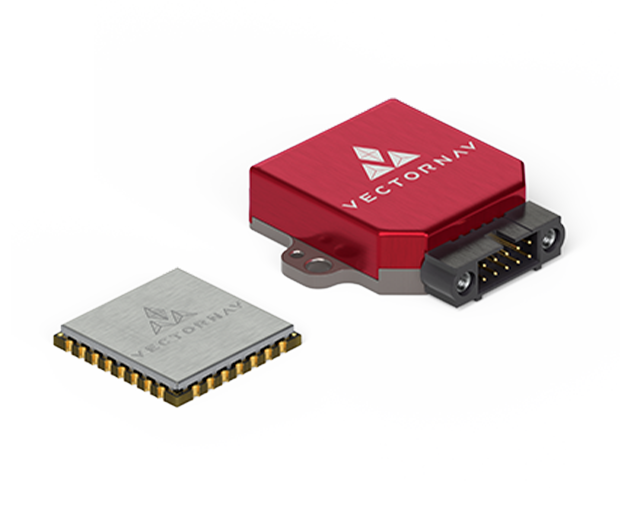
\includegraphics[width = 4cm, height = 6cm]{vn-100-smd-rugged_new.png}};
			\begin{scope}[x={(image.south east)},y={(image.north west)}]
				\draw[color=black, ultra thin,fill=white] (0.0,0.0) rectangle (0.21,0.16) node[pos=.5] {A};
			\end{scope}
		\end{tikzpicture}
	\end{subfigure}
	\hfill
	\begin{subfigure}[t]{.3\textwidth}
		\begin{tikzpicture}
			\node[anchor=south west,inner sep=0] (image) at (0,0) { 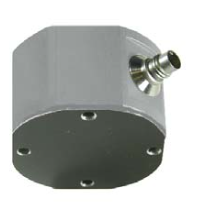
\includegraphics[width = 4cm, height = 6cm]{servokbeam.PNG}};
			\begin{scope}[x={(image.south east)},y={(image.north west)}]
				\draw[color=black, ultra thin,fill=white] (0.0,0.0) rectangle (0.21,0.16) node[pos=.5] {B};
			\end{scope}
		\end{tikzpicture}
	\end{subfigure}
	\hfill
	\begin{subfigure}[t]{.3\textwidth}
		\begin{tikzpicture}
			\node[anchor=south west,inner sep=0] (image) at (0,0) { 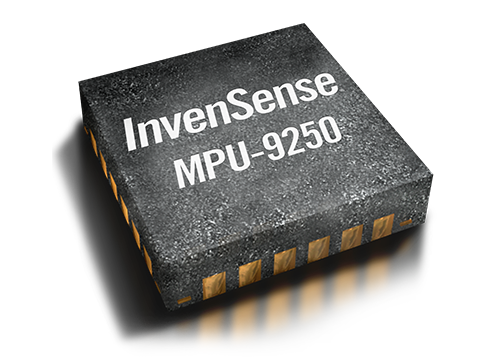
\includegraphics[width = 4cm, height = 6cm]{rp-mpu-9250.png}};
			\begin{scope}[x={(image.south east)},y={(image.north west)}]
				\draw[color=black, ultra thin,fill=white] (0.0,0.0) rectangle (0.21,0.16) node[pos=.5] {C};
			\end{scope}
		\end{tikzpicture}
	\end{subfigure}
	\hfill
	\label{fig:imus}
	\caption{Diagram showing examples of the different types of inertial measurement systems (IMUs) available for commercial use such as (A) an Attitude Heading Reference System (AHRS) VN100 \cite{vn-100} used by \cite{rabault2019open}, (B) an analog capacitive accelerometer 8330B3 Servo-KBeam accelerometer used by \cite{kohout2015device} \cite{kistlerIMU} and (C) a 9 degree of freedom MPU9520 \cite{mpu9520} used by \cite{kohout2015device}. }
\end{figure}

\textcite{ahmad2013reviews} show that package size can limit the applications of the IMU. Additionally, IMUs require careful calibration and filtering in order to reduce the effects of bias offsets as well as low and high frequency drift \cite{fong2008methods}. More advanced filtering methods have been developed to improve the accuracy of IMUs such as Kalman filters \cite{simon2001kalman}  for positional estimates or Real-Time Kinetic Fusion (RTK) for velocity \textcite{meng2014optimal}. While important to the integrity of IMU data, these methods are usually implemented in software which is discussed in the upcoming sections. Finally, the degrees of freedom (DoF) influences the application of the IMU. The magnetometer is used to improve the accuracy of the gyroscope measurement and account for low frequency noise (drift) \cite{ahmad2013reviews}. However, removing the magnetometer is sensitive to magnetic distortion which can affect the measurements. \textcite{kohout2015device} encountered magnetic distortion during the SIPEX II deployments in September 2012 which rendered the magnetometer readings useless. In this section, the IMU is integral to deriving a time-series representation of inertia to calculate wave data as described above however, another application relevant to the literature is using IMUs to improve navigation \cite{ahmad2013reviews}. An IMU can be coupled with a Global Positioning System (GPS) device to determine position in areas with poor signal which can assist greatly with determine ice drift (discussed in section \ref{sec:ch2_drift}). Based on these considerations, table \ref{tab:imu_component} shows the IMU component selection for each device.
 
%TODO add table

\begin{table}[H]
	\centering
	\setlength{\extrarowheight}{5pt};
	\caption{Comparison of the inertial measurement systems selected for each device showing the sensors included as well as the degrees of freedom.}
	\label{tab:imu_component}
	\resizebox{\textwidth}{!}{%
		\begin{tabular}{|l|l|l|c|l}
			\cline{1-4}
			\textbf{Device name} & \textbf{Inertial Measurment Unit} & \textbf{Sensors} & \textbf{Degrees of freedom} &  \\ \cline{1-4}
			\multirow{3}{*}{WIIB} & \multirow{3}{*}{VN-100} & Accelerometer & \multirow{3}{*}{9} &  \\ \cline{3-3}
			&  & Gyroscope &  &  \\ \cline{3-3}
			&  & Magnetometer &  &  \\ \cline{1-4}
			\multirow{4}{*}{WIIOS} & 8330B3 Servo-KBeam & Vertical Acceleration & 1 &  \\ \cline{2-4}
			& \multirow{3}{*}{MPU9250} & Accelerometer & \multirow{3}{*}{9} &  \\ \cline{3-3}
			&  & Gyroscope &  &  \\ \cline{3-3}
			&  & Magnetometer &  &  \\ \cline{1-4}
			\multirow{3}{*}{NDWB} & \multirow{3}{*}{IG-500N} & Accelerometer & \multirow{3}{*}{9} &  \\ \cline{3-3}
			&  & Gyroscope &  &  \\ \cline{3-3}
			&  & Magnetometer &  &  \\ \cline{1-4}
			SKIB & LIS3DH & Accelerometer & 3 &  \\ \cline{1-4}
			\multirow{3}{*}{SIMB} & \multirow{3}{*}{BNO055} & Accelerometer & \multirow{3}{*}{9} &  \\ \cline{3-3}
			&  & Gyroscop &  &  \\ \cline{3-3}
			&  & Magnetomer &  &  \\ \cline{1-4}
			Polar ISVP & None & - & - &  \\ \cline{1-4}
			Trident & None & - & - &  \\ \cline{1-4}
		\end{tabular}
		}
\end{table}

As mentioned previously, systems such as WIIOS and WIIB have built their purpose around wave measurements and therefore have specified high powered, high accuracy IMUs for wave measurements. However, WIIOS buoy separates itself from WIIB by having a cheaper complimentary 9 dof IMU to complement the measurements \cite{kohout2015device}. SWIFT Buoy and the NDWB buoy use an integrated system known as an Inertial Navigation System (INS) with the former containing an SBG Elipse AHRS \cite{thomson2012wave} and the latter containing a IG-500-A1G2 \cite{doble2017robust}. This device contains a GPS and an Onboard processor for RTK fusion and Kalman filtering whereas other devices use an external processor for filtering. The SIMB Buoy is the only buoy on the list that has an IMU for non-wave related measurements. It uses a cheaper Bosch BNO055 which is used solely for measuring the orientation of the device.

\subsubsection{Software processing}

An IMU is a power device however extensive software proccessing is required to extract key parameters \cite{ahmad2013reviews}. Examples of software processing algorithms are shown in \textcite{kuik1988method} and \textcite{earle1996nondirectional}\footnote{See Appendix \ref{welchearl}.} for wave processing algorithms. Additionally, as mentioned previously, advanced filtering techniques are required to reduce the effects of low and high frequency noise. In this subsection the software processing strategy for each device given for extracting the desired parameters shown in table \ref{tab:device_deployment}.

\begin{table}[H]
	\centering
	\label{key}
	\caption{Comparison of sampling strategies implemented in each device. This includes the desired measurands, sample rate and sample period of each IMU session}
	\setlength{\extrarowheight}{5pt}
	\resizebox{\textwidth}{!}{%

		\begin{tabular}{|l|l|l|l|}
			\hline
			\textbf{Device name} & \textbf{Degree of Freedom used} & \textbf{Sample rate} & \textbf{Sample Period} \\ \hline
				\multirow{3}{*}{WIIB} & Vertical Acceleration & \multirow{3}{*}{10 Hz} & \multirow{3}{*}{25 minutes} \\ \cline{2-2}
				& Pitch &  &  \\ \cline{2-2}
				& Roll &  &  \\ \hline
				\multirow{4}{*}{WIIOS} & 3-axis acceleration & \multirow{4}{*}{2 Hz} & \multirow{4}{*}{11 minutes} \\ \cline{2-2}
				& 3-axis gyroscope &  &  \\ \cline{2-2}
				& 3-axis magnetometer &  &  \\ \cline{2-2}
				& Vertical  analog acceleration &  &  \\ \hline
				\multirow{5}{*}{NDWB} & 3-axis acceleration & \multirow{5}{*}{1 Hz} & \multirow{5}{*}{Continuous} \\ \cline{2-2}
				& 3-magnetometer &  &  \\ \cline{2-2}
				& heave &  &  \\ \cline{2-2}
				& roll &  &  \\ \cline{2-2}
				& pitch &  &  \\ \hline
				SKIB & 3-axis acceleration & 25 & 10 minutes \\ \hline
				\multirow{3}{*}{SWIFT} & 3-axis acceleration & \multirow{3}{*}{5} & \multirow{3}{*}{9 minutes} \\ \cline{2-2}
				& Tilt &  &  \\ \cline{2-2}
				& Horizontal Rotation &  &  \\ \hline
				\multirow{2}{*}{SIMB} & Tilt & \multirow{2}{*}{-} & \multirow{2}{*}{-} \\ \cline{2-2}
				& Orientation &  &  \\ \hline
			\end{tabular}
			}
		\end{table}

\textcite{rabault2019open} extract wave parameters by passing the raw time series data through an Extended Kalman Filter running at 800 Hz then through a low pass filter. Wave spectral data is calculated using the method by \textcite{earle1996nondirectional} where Co-spectra was calculated using the method by \textcite{kuik1988method}. Significant wave height wass calculated through double integration using a Fast Fourier Transform. sampling is performed at 10 Hz to satisfy the nyquist sampling criteria for open ocean waves as described in \cite{rabault2019open,earle1996nondirectional}.

\textcite{kohout2015device} however, opted for a reduced sampling rate of 2 Hz over a shorter sample time. This was achieved by oversampling IMU data at 640 Hz then down-sampling the data through a multistage decimator \cite{kohout2015device}. Before each decimation, data was filtered using a Butterworth filter at 8 Hz with a cut-off frequency of 2 Hz, then once again at 40 Hz. Significant wave height is calculated by double integration using the Welch-Earl method \cite{earle1996nondirectional,welch1967use} multiplying the transformed data set by a response weighted function to remove low frequency drift. Finally, the Longuet-Higgens parameters are calculated thereby characterizing wave in ice activity.

\textcite{doble2017robust} did not apply any data processing algorithm to the raw time series as it is transmitted directly over iridium. However, the raw time series is filtered using an Extended Kalman Filter running at 10 Hz.

The SKIB collects data from a sample window which is processed using a classical RC filter to attenuate frequencies below 0.04 Hz.Thereafter, \textcite{earle1996nondirectional} spectra and Co-spectra calculation are then applied.

The SWIFT buoy is the only device that used multiple sensor types for sea state calculation. Additionally, data was collected more frequently in short intervals (9 minute sample periods every 12 minutes) which include Doppler profiles, camera images and IMU data. The inertial navigation system (INS) outputted a real-time kinematic (RTK) fusion data set where IMU data was passed through a Coning \& Sculling Extended Kalman Filter running at 1 KHz \cite{thomson2012wave} while the doppler profiler was sampled at 8 Hz. Turbulence profile was calculated through time-averaging and data fitting of the Doppler profile. Then, the ocean current state was calculated using the Stokes drift equation over a time-averaged velocity series. Finally, wave data was calculated  through image processing from a still of the sea state taken from an onboard camera.

\par{SIMB}

The SIMB uses the IMU in a non-critical manner. The device transmits tilt and orientation metadata \cite{planck2019evolution} describing the current status of the SIMB. While no method has been described by \textcite{planck2019evolution} to calculate tilt, it can be achieved by measuring the orthogonal acceleration values over an angle of ration and taking the inverse tangent of the resulting value for each axis \cite{tuck2007tilt}.


Therefore IMUs are integral for performing sea state calculations and measuring wave spectra, a sufficient processor is required to filter and process the data therefore, significant consideration should be given to coupling a powerful processor with a sufficiently powerful inertial measurement unit.

\subsection{Measurement of Ice drift using GPS}
\label{sec:ch2_drift}

This sections discusses the technology and techniques used for determining ice drift. The predominant approach towards understanding modeling ice drift is by using the techniques presented by \textcite{hibler1979dynamic}\footnote{See Numerical Modeling in Appendix \ref{app:modelling}} where kinematic data is used to study ice drift dynamics and calibrate the ice drift model. Additionally, \textcite{lepparanta2001sea} present two methods for collecting ice drift data. The first method utilises measurement beacons are attached to the ice floes and used to track trajectories. The second method uses imaging devices such as radar, and satellites to determine ice displacement \cite{lepparanta2001sea}.\par

The discussion of modern technology for ice observations from chapter \ref{sec:ch1.section1} showed that observations from satellites such as OSI-SAF and METSAT are unsuitable for measurements \cite{lepparanta2001sea,galin2011validation} due ti their low spatial resolutions. Hence, a need arises for in situ drift measurement devices. Global positioning systems (GPS) have been the standard for ice drift measurements \cite{lepparanta2001sea} as they are capable of measuring data at relatively high temporal resolutions ranging from 15 minutes \cite{alberello2019drift} to 25 minutes \cite{rabault2019open} as opposed to the limit of 3 hours \cite{alberello2019drift}. This section provides an overview of GPS technology and how the devices have implemented it for measuring positional or drift data.

\subsubsection{Overview of GPS}

The principles that govern GPS have remained unchanged since its inception in 1973 \cite{spilker1996global}. The system consists of a satellite constellation that constantly broadcast their estimated position. A GPS device determines its position by matching a user-generated signal to that of four received satellites and comparing the phase difference to an on-board crystal oscillator \cite{spilker1996global}. This technique is called ranging and four satellites spread in a uniform geometry will allow for a device to calculate latitude, longitude, altitude and time to a relative degree of accuracy. The number of unknown signals correlates to the number of satellites required. Generally, a GPS device will have a lesser degree of accuracy than the satellites. Hence, an incoming signal can be used to correct the device's clock \footnote{provided altitude or time are already known \cite{spilker1996global}}.To accurately predict the satellite's trajectory, satellite ranging is performed by a network of global monitoring which calculate the future position and send it back to the satellite. GPS signals are transmitted on two frequencies: 1575.42 MHz and 1227.46 MHz\cite{spilker1996global}. These are synchronously generated signals and allow a device to correct for ionospheric distortion. These bands carry modulated signals which are as follows: \cite{spilker1996global}


\begin{enumerate}
	\item Clear Acquisition Code:  This is a short code transmitted at 1.023 MHz and is used to request the Standard Positioning Service or SPS.
	\item Precise (P) Code: this is a much longer acquisition code. This signal is transmitted at 10.23MHz which is 10 x the rate of a CA code. This results in a much more accurate signal with less noise. This signal allows for the acquisition of Precise Positioning Service. However, this service is not available to unauthorized users and cannot be spoofed. As a result, this signal requires additional decryption.    
\end{enumerate}

\textcite{spilker1996global} also mention that military operators can degrade GPS signals which result in decreased accuracy from 20 m up to 100 m. The reduction of these accuracies requires differential GPS techniques, however, due to the scope of this projects, this section will not be explored any further.Finally, once the acquisition signal is transmitted, the GPS device begins modulating at 50 bit/s. This allows the satellite to transmit its position as well as clock correction information to the device.\par

The GPS satellite constellation consists of 24 GPS satellites. These are configured into three rings of eight satellites orbiting at different latitudes. These orbital altitudes were selected as 10.98 Nautical Miles \cite{spilker1996global}. This altitude was chosen to optimise user visibility with the number of crossings over United Sates ground stations, and cost of launching the satellites \cite{spilker1996global}. These satellites carry onboard atomic clocks for stability at $1\times10^{13}$ resolution. This allows for extremely accurate signaling as well as allowing for much more predictable time and position signals \cite{spilker1996global}. To achieve this, these atomic clocks are made out of either Cesium or Rubidium. Also, a frequency correction at $4.5\times10^{10} \text{ } Hz$ is provided to correct for relative shifts. \par

\subsubsection{GPS Error Modeling}

As mentioned in the previous section,GPS signal accuracy is greatly affected by earth effects and satellite distribution. The main source of distortion is attributed to the earth's ionosphere \cite{spilker1996global}. The ionospheric free electronics cause a delay in the modulated signal which is proportional to the sum of electrons along the signal's trajectory and inversely proportional to the signal's frequency squared. This delay is modeled as the product of a theoretical $90^\circ$ delay (Zenith delay) and a function of the elevation angle (obliquity factor). This results in a ratio of between 1.0 to 3.0 at small elevation angles \cite{spilker1996global}. This results in delays of 3 m (often at night) to 20 m (after midday).These delays result in errors in positional accuracy as shown in figure \ref{fig:DOP_effects} which can increase the measurement confidence interval resulting in an unreliable positional reading \cite{spilker1996global}. Fortunately,These delays are usually resolved by satellite correlated positions.

\begin{figure}[H]
	\centering
	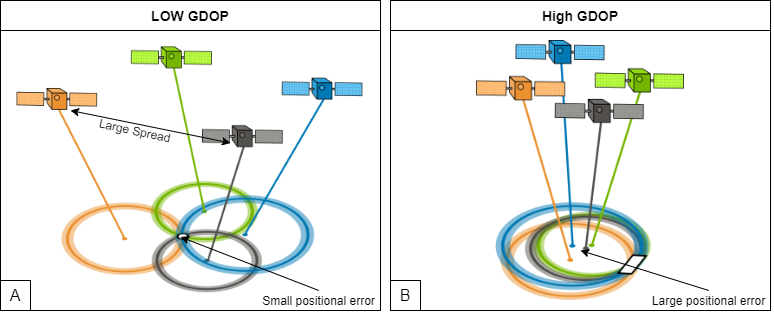
\includegraphics[width =\linewidth]{DOPeffect.png}
	\caption{Diagram showing how satellite distribution affects the positional estimation. GNSS Satellites have an associated inaccuracy which is represented by the circles. Locking on to more than one satellite reduces these inaccuracies by interpolating the position from the phase differences between satellites. This value is greatly affected by the spread of satellites as a larger spread results in a more accurate positional estimate (A) while a shorter satellite spread results in a less accurate positional estimate. A measure of this inaccuracy is called the dilation of procession (DOP). Figure was adapted from images by \cite{GISGeo2020DOP} for A and B.}
	\label{fig:DOP_effects}
\end{figure}

 Correction can be performed in one of two ways:
\begin{enumerate}
	\item Transmission of Ionospheric model parameters as part of the message to the device and calculating the offset using that
	\item Using the two previously mentioned transmission frequencies directly measuring the delays in each broadcast frequency and estimating the position using the equation:\cite{spilker1996global}
	\begin{equation}
		1.546(delay_{L1} - delay_{L2})
	\end{equation}
\end{enumerate}

Navigation errors are characteristic of GPS performances. These errors are affected significantly by satellite spread and ranging errors. Assuming the incoming signal is uncorrelated with a mean of zero, the RMS positional error is calculated as:
\begin{equation}
	RMS_{error} = (\text{Geometric Dilution})(\text{RMS Ranging errors})
\end{equation}

The geometric dilution is modeled by estimating the processional dilution of the spatial and temporal dimension measurements. This value estimates the quality of the GPS signal and is inversely proportional to the volume of the shape formed by 4 satellite \cite{jwo2001efficient}. \textcite{jwo2001efficient} outlines the procedure for the calculation of this value. Given a user's position on the earth, the distance from the user to the satellite is characterised by the equation:
\begin{equation}
	r =  s - u
\end{equation}
where $r$ is the distance from the user to the satellite, $s$ is the distance from the earth's centre to the satellite and u is the distance from the earth to the user. By measuring the propagation time from the user to the satellite, The absolute distance $||r||$ can be calculated and hence, the pseudo-range can be calculated as
\begin{equation}
	\rho_i = ||s_i-u||+ct_b + v_{\rho_i}
\end{equation}
where $\rho_i$ is the pseudorange for satelite i, c is the speed of light, $t_b$ is  the clock offset and $v_{\rho_i}$ is the noise of the pseudorange measurement and:
\begin{equation}
	||s_i-u|| = \sqrt{(x_i - x_u)^2+(y_i-y_u)^2+(z_i-z_u)^2} \text{ for } i \in 1,2,3...N \label{los}
\end{equation}
where $N$ is the number of satellites and $(x_i,y_i,z_i)$ is the 3 dimensional position of satellite $i$. This represents a non-linear relationship for the line of sight of a satellite.  \textcite{jwo2001efficient} explains that by creating a Taylor series centered on a nominal user position $(\hat{x_n},\hat{y_n},\hat{z_n})$ and ignoring the higher terms \cite{jwo2001efficient}. It then follows that:
\begin{equation}
	\Delta\rho_i = \rho_i - \hat{\rho_i} = e_{i1}\Delta x_u + e_{i2}\Delta x_u +  e_{i3}\Delta z_u
\end{equation}

The terms $e_{ij}$ represent the line of sight vector $E_i$ whereas the term $\hat{\rho_i}$ is the pseudo-range at the nominal user's position. It follows that the vector $E_i$ can be calculated as follows \cite{jwo2001efficient}.
\begin{subequations}
	\begin{align}
		e_{i1} = \frac{\hat{x_n} - x_i}{\hat{r_i}}\\
		e_{i2} = \frac{\hat{y_n} - y_i}{\hat{r_i}}\\
		e_{i3} = \frac{\hat{z_n} - z_i}{\hat{r_i}}\\
		\hat{r_i} = \sqrt{(\hat{x_n} - x_i)^2+(\hat{y_n} -y_i)^2+(\hat{z_n} -z_i)^2}
	\end{align}
\end{subequations}

Given $n$ satellites, the equation \eqref{los} can be written as a matrix with the following form:
\begin{equation}
	\textbf{z} = \textbf{Hx}+ \textbf{v}
\end{equation}
\begin{equation}
	\Delta \rho _i = \begin{bmatrix}
		\Delta \rho_1 &  \Delta \rho_2 &  \Delta \rho_3 & ... & \Delta \rho_n
	\end{bmatrix} 
\end{equation}
where 
\begin{subequations}
	\begin{align}
		\textbf{H} = \begin{bmatrix}
			e_{11} & e_{12} & e_{13}& 1 \\
			e_{21} & e_{22} & e_{23}& 1 
			\\
			e_{31} & e_{32} & e_{33}& 1
			\\
			... & ... & ... &  1 
			\\
			e_{n1} & e_{n2} & e_{n3} & 1
		\end{bmatrix}\\
		\textbf{x} = \begin{bmatrix}
			\Delta x_u \\ \Delta y_u \\\Delta z_u \\ c\Delta t_b
		\end{bmatrix}\\
		\textbf{v} = \begin{bmatrix}
			v_{\rho_1}\\
			v_{\rho_2}\\
			v_{\rho_3}\\
			...\\
			v_{\rho_n}
		\end{bmatrix}
	\end{align}
\end{subequations}

The Matrix \textbf{H} is $n\times4$ where $n \geq 4$ to calculate all the parameters for GDOP \cite{jwo2001efficient}. We can then solve for the vector \textbf{x} by taking the psuedo inverse of H i.e $\hat{\textbf{x}} = (\textbf{H}^T\textbf{H})^{-1}\textbf{H}^t\textbf{z}$. Hence, given that the psuedo range is linearised, the quality of navigation is taken as the difference between the estimated position and the actual position \cite{jwo2001efficient}.
\begin{equation}
	\Tilde{\textbf{x}} = \hat{\textbf{x}} - x = (\textbf{H}^T\textbf{H})^{-1}\textbf{H}^Tv
\end{equation}
$E\{\Tilde{\textbf{x}}\Tilde{\textbf{x}}^T\}$ describes the covariance between the errors in the components of the estimated position \cite{jwo2001efficient} and is calculated as 
\begin{equation}
	E\{\Tilde{\textbf{x}}\Tilde{\textbf{x}}^T\} = (\textbf{H}^T\textbf{H})^{-1}\textbf{H}^TE\{\textbf{vv}^T\} (\textbf{H}^T\textbf{H})^{-1}\textbf{H}
\end{equation}
where $E\{\textbf{vv}^T\} = \sigma^2 I$. If all components of $\sigma$ are uncorrelated then the covariance becomes 
\begin{equation}
	E\{\Tilde{\textbf{x}}\Tilde{\textbf{x}}^T\} = \sigma^2(\textbf{H}^T\textbf{H})^{-1}
\end{equation}
and thus the GDOP factor can be calculated from the RMS values of $\sigma^2$ i.e.
\begin{equation}
	GDOP = \frac{\sqrt{\sigma_{xx}^2+\sigma_{yy}^2+ \sigma_{zz}^2+\sigma_{tt}^2}}{\sigma}
\end{equation} where $\sigma_{xx}^2$,$\sigma_{yy}^2$,$\sigma_{zz}^2$,$\sigma_{tt}^2$ are the RMS values of the x,y,z time components respectively. THe value GDOP can also be decomposed into the positional dilation of precision (PDOP), time dilation of precision (TDOP), horizontal dilation of precision HDOP, and vertical dilation of precision (VDOP) which characterise the effects satellite spread on the 3 dimensional position, time, horizontal position and altitude respectively.\par

Ranging errors are shown to come from 6 sources \cite{spilker1996global}:
\begin{enumerate}
	\item Satelite ephemeris
	\item Satelite clock
	\item Ionospheric group delay
	\item Trophospheric group delay
	\item Multipath scattering
	\item Hardware/software errors
\end{enumerate}

These errors need to be accounted for in order to produce an accurate, reliable position.

\subsubsection{GPS Component Selection}

The component selection for each device is shown in table \ref{tab:dev_gps} below.

\begin{table}[H]
	\centering
	\caption{Comparison between different GPS devices, sampled data and periods between samples implemented by each device.}
	\label{tab:dev_gps}
	\setlength{\extrarowheight}{5pt}
	\resizebox{\textwidth}{!}{% 
	\begin{tabular}{|l|l|l|l|}
		\hline
		\textbf{Device Name} & \textbf{GNSS Device} & \textbf{Data Sampled} & \textbf{Period between Samples} \\ \hline
		WIIB & MTK3339 & Geographical position & 25 minutes \\ \hline
		\multirow{2}{*}{WIIOS} & \multirow{2}{*}{MTK3339} & Latitude (decimal degrees) & \multirow{2}{*}{3 hours} \\ \cline{3-3}
		&  & Longitude (decimal degrees) &  \\ \hline
		NDWB & SkyTraq S1351R & Geographical position & 1 hour \\ \hline
		SKIB & MTK3339 & Geographical postion & 10 minutes \\ \hline
		\multirow{2}{*}{SWIFT} & \multirow{2}{*}{Qstarz BT-Q1000eX} & Geographical position & \multirow{2}{*}{200 ms} \\ \cline{3-3}
		&  & Horizontal velocity &  \\ \hline
		SIMB & MTK3339 & Geographical position & 1 hour \\ \hline
		Polar ISVP & Jupiter F2 Module & Geographical position & 3 hours \\ \hline
		\multirow{3}{*}{Trident} & \multirow{3}{*}{Unspecified GPS} & \multirow{3}{*}{Geographical position} & 0 - 5 minutes \\ \cline{4-4} 
		&  &  & 5 - 60 minutes \\ \cline{4-4} 
		&  &  & 1 - 24 hours \\ \hline
	\end{tabular}	
	}
	
\end{table}
Table \ref{tab:dev_gps} above shows the GPS receivers implemented in each system as well as measurements of interest. The most common gps is the MTK3339, a gps module developed by adafruit (cite). Additionally, all devices have fixed transmission periods between samples except the Trident buoy which has user configurable periods that can be set from a couple of minutes to full hours. Most devices use the GPS for positional location however, SWIFT buoy measures horizontal velocity in addition to vertical position\cite{thomson2012wave}. \textcite{thomson2012wave} justify this by stating that the accuracy of horizontal velocity measured by a gps is accurate enough ($\pm 0.5 \text{ }m\cdot s^{-1}$)to be used for determining the orbital motions of waves. \textcite{kohout2015device} and \textcite{rabault2019open} provide the measurements recorded by the GPS however, very little discussion is given regarding the performance of the device. \textcite{doble2017robust} showed that during their year long deployment, 14 buoys maintained a near perfect satellite signal acquisition however, software issues with the GNSS reciever resulted in a failure to obtain measurements in 5 systems. However, \textcite{doble2017robust} had implemented two-way iridium communication and were able to partially overcome this set back by transmitting commands that performed a software reset on the GPS receiver. Additionally, two devices lost signal for 6 days while another two devices lost signal for 62 days and 41 days respectively \cite{doble2013wave}. This shows that acquisition failures can cause temporal gaps in data and therefore, need to be reduced in order to provide robust data sets.

Each ice floe follows a unique trajectory \cite{lepparanta2001sea}  and individual trajectories combine to form a continuum. It has previously been believed that sea ice drift has been linked strongly to significant wave events \cite{alberello2019drift}. An experiment was conducted by \textcite{alberello2019drift} to measure the drift of sea ice during a cyclone event. Here it was found that wind velocity is the dominant driver of sea ice drift \cite{alberello2019drift} causing ice drifts of up to $0.75\text{ } m\cdot s^{-1}$ \cite{alberello2019drift}. Sea ice drift speed is extremely sensitive to sampling rates. \cite{alberello2019drift} where sampling rates of 6 hours can underestimate the ice velocity by 5\% \cite{alberello2019drift} and up to 20\% for 12-hour sample rates. The consequence is reduced, near unusable, estimates of sea ice velocity components as well as drag coefficient and wind factor estimates. High temporal resolutions are capable of capturing important, inter-daily activities such as ice oscillations. \textcite{alberello2019drift} state that to accurately capture Sea ice dynamics, a temporal resolution of at least 3 hours is required \cite{alberello2019drift}. Table \ref{tab:dev_gps} shows that all devices sample GPS at a rate of 3 hours or less thereby fulfilling this criteria This not only allows for the capture of accurate drift speeds but provides an accurate characterization of instantaneous velocities and Coriolis forces \cite{alberello2019drift}.
 
\subsection{Temperature Sensing and Measurement}

As discussed in Chapter \ref{sec:ch1.section1}, Antarctic sea ice follows a unique formation cycle with different phases marked by changes in season. Sea ice formation additionally is affected by environmental factors which can arise from one of two sources: Long-period seasonal cycles \cite{barber2005microwave} which affect snow growth and sea ice formation, and short term extreme weather events \cite{vichi2019effects,albarello2020drift} which affect the thermodynamics of the formed ice and results in ice drift and collisions \cite{arrigo2004large}. One key measurement for correlating environmental effects to sea ice formation is air temperature. \textcite{barber2005microwave} show that  the melting and freezing phases in the sea ice life cycle is preceded by increases in air temperature above freezing and decreases in temperature below freezing respectively. In addition, \textcite{vichi2019effects} show that warmer air temperatures were observed during polar events. This shows that temperature is critical measurement for understanding sea ice lifecylces and the effects of ocean procesess. Additionally \textcite{kohout2015device,doble2017robust,doble2017robust} have discussed the significance of sea ice melting. This was considered a significant phase of sea ice and was classified as a phase in the development of their buoy. Hence, we turn to temperature sensing as a solution to understanding the effects of temperature on Antarctic sea ice.\par 

\begin{figure}[H]
	\centering
	\begin{subfigure}[b]{0.3\textwidth}
		\begin{tikzpicture}
			\node[anchor=south west,inner sep=0] (image) at (0,0) { 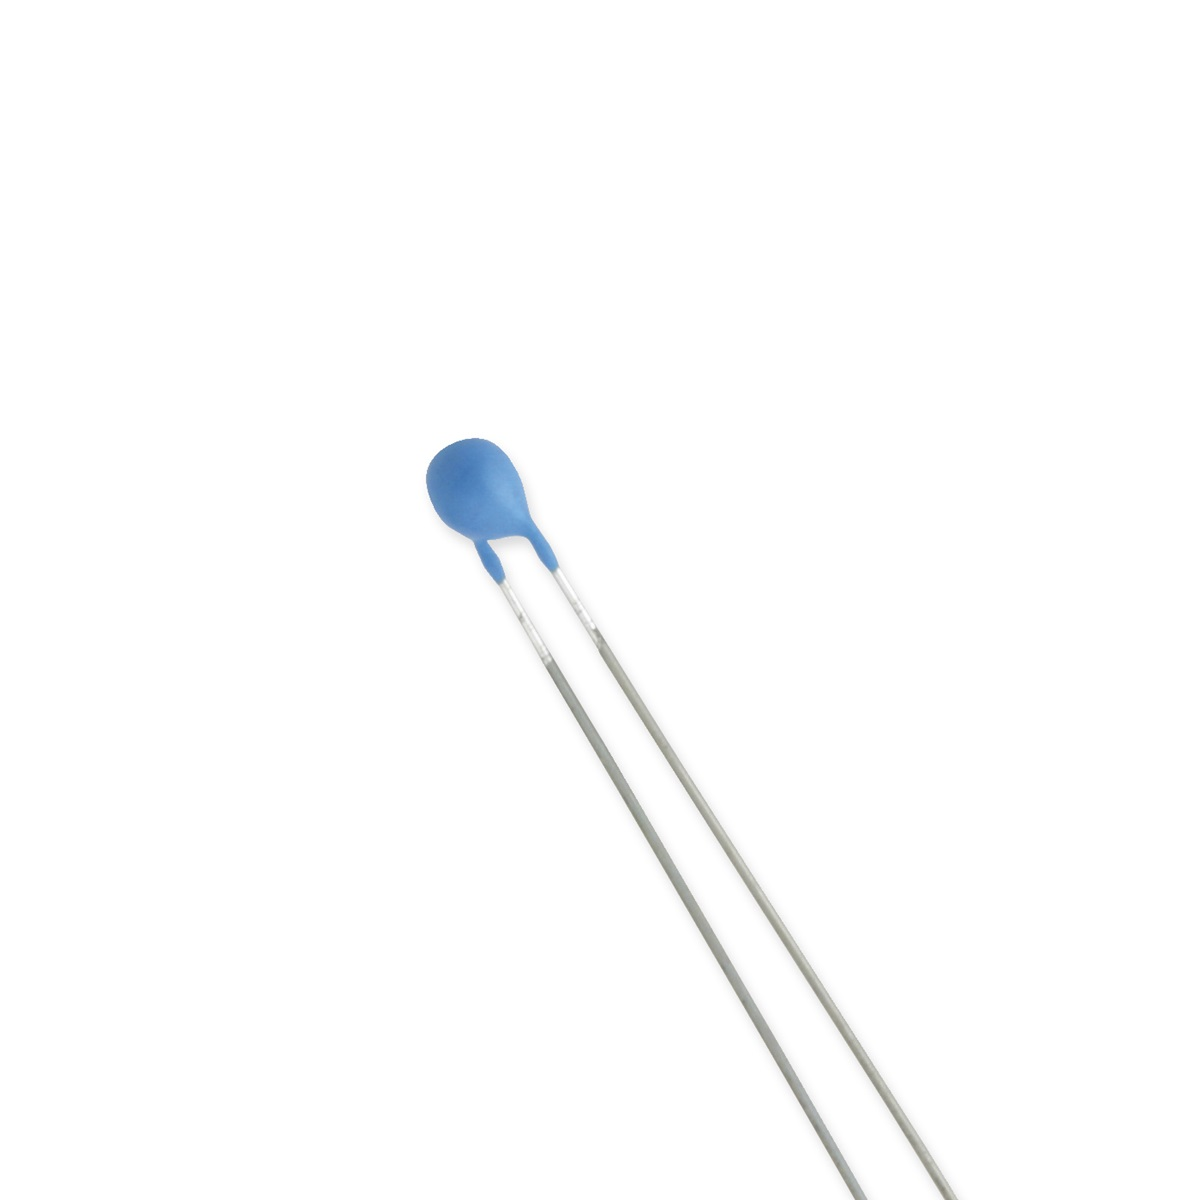
\includegraphics[width = 3cm,height=3cm]{pr303J2.jpg}};
			\begin{scope}[x={(image.south east)},y={(image.north west)}]
				\draw[color=black, ultra thin,fill=white] (0.0,0.0) rectangle (0.21,0.16) node[pos=.5] {A};
			\end{scope}
		\end{tikzpicture}
	\end{subfigure}%
	\hfill
	\begin{subfigure}[b]{0.3\textwidth}
		\begin{tikzpicture}
			\node[anchor=south west,inner sep=0] (image) at (0,0) { 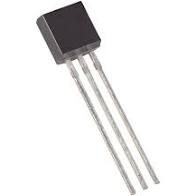
\includegraphics[width = 3cm,height=3cm]{ds18b20.jpg}};
			\begin{scope}[x={(image.south east)},y={(image.north west)}]
				\draw[color=black, ultra thin,fill=white] (0.0,0.0) rectangle (0.21,0.16) node[pos=.5] {B};
			\end{scope}
		\end{tikzpicture}
	\end{subfigure}%
	\hfill
	\begin{subfigure}[b]{0.3\textwidth}
		\begin{tikzpicture}
			\node[anchor=south west,inner sep=0] (image) at (0,0) { 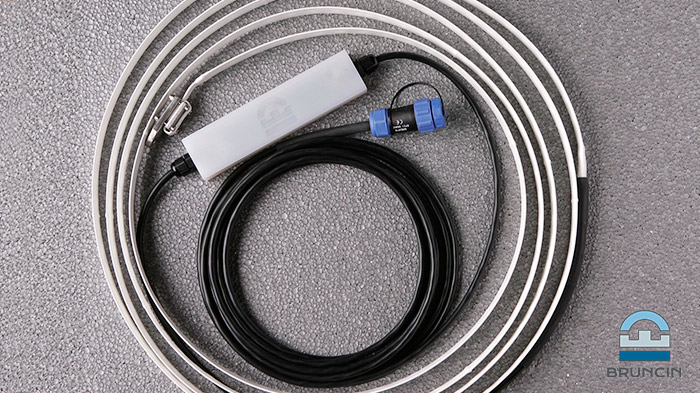
\includegraphics[width = 3cm,height=3cm]{temperature-chain-bruncin-1.jpg}};
			\begin{scope}[x={(image.south east)},y={(image.north west)}]
				\draw[color=black, ultra thin,fill=white] (0.0,0.0) rectangle (0.21,0.16) node[pos=.5] {C};
			\end{scope}
		\end{tikzpicture}
	\end{subfigure}%
	\hfill
	\caption{Examples of temperature sensors employed by remote sensing devices.These types of devices include (A) thermistors such as the PR303J2 (image source: \cite{pr303J2}), (B) digital temperature sensors such as the DS18B20 (image source: \cite{ds18b20}) and (C) digital temperature chains (DTC) such as the Bruncin DTC (image source: \cite{bruncindtc}) } 
	\label{fig:temp_examples}
\end{figure}

Temperature sensing technology is commonly used for thermal compensation as measurements such as pressure and humidity are dependent on environmental temperature \cite{mansoor2015silicon}. Thermal sensing technology exists in a variety of forms however, choice of sensor is heavily dependant on the application i.e. the object to be measured, the material state and the type of contact with the sensor \cite{mansoor2015silicon,childs2000review}. There are 3 main categories of measurement techniques \cite{childs2000review}:

\begin{enumerate}
	\item Invasive Measurements: Direct contact with an object of interest. This method is suitable for the measurement of objects in liquid or gas states. This category encompasses thermoelectric devices, liquid in glass thermometers, electronically resistive devices as well as semiconductor devices \cite{mansoor2015silicon}
	\item Semi-Invasive: Using the thermal measurement medium on an object and observing the effects of temperature such as thermal paints. Note: measurements are not directly taken from the object but rather the properties of the medium.
	\item Non-Invasive: Object is measured from a distance using a device such as an infrared camera or acoustic thermography.
\end{enumerate}

In addition, sensor selection is based on the range, accuracy, resolution and precision of the device to ensure correct use An overview of different electric sensors is given below \cite{childs2000review} A full discussion of the types of sensors is provided below where the types of technology, advantages and disadvantaeges are provided. Additionally, the technology has been selected for its implementation in the remote sensing devices shown in table \ref{tab:device_tempsense} below.
 
\begin{table}[H]
	\centering
	\caption{Comparison of the different components used by each device for temperature measurement as well as the . Each device measures temperature of a different process. For example:  the WIIB measure air temperature whereas a device like the SIMB measures temperature profiles of ice floes in addition to air temperature.}
	\label{tab:device_tempsense}
	\setlength{\extrarowheight}{5pt}
	\resizebox{\textwidth}{!}{%
	\begin{tabular}{|l|l|l|l|}
		\hline
		\textbf{Device name} & \textbf{Temperature sensor} & \textbf{Sensor type}& \textbf{Measurement Objective} \\ \hline
		WIIB & VN-100 & Digital Tempereture sensor & Air temperature \\ \hline
		WIIOS & DS18B20 & Digital temperature sensor & Air temperature \\ \hline
		NDWB & IG-500 & Digital temperature sensor &Internal ambient temperature \\ \hline
		SKIB & None & none & None \\ \hline
		SWIFT & Aquadop profiler & Thermistor & water temperature \\ \hline
		\multirow{2}{*}{SIMB} & DS18B20 & Digital temperature sensor & Air Temperature \\ \cline{2-3} 
		& Bruncin DTC & Digital temperature chain&Ice temperature profile \\ \hline
		Polar ISVP & PR303J2 & thermistor &Sea surface temperature \\ \hline
		Trident & unspecified & Not reported &Air temperature \\ \hline
	\end{tabular}
}
\end{table}

Table \ref{tab:device_tempsense} shows that the majority of devices use digital temperature sensors for ambient air temperature measurementwith thermistors begin the second temperature sensors type as used by \textcite{thomson2012wave}. Most device use temperature sensors that have been integrated into high powered IMU/AHRS systems as is the case with WIIB and NDWB. While the SWIFT buoy and the Polar ISVP both utlise the same sensing technology however the Polar ISVP used a standalone PR303J2 while the SIFT used the temperature sensor onboard the Nortek Aquadopp Profiler which is primarly a current profiler. This shows that temperature sensing was not a primary focus for this device design and this is supported by the lack of discussion regarding the performance of the temperature sensor in the literature.
\subsubsection{Thermistors}

Modern thermistors have progressed significantly in the past decade. Up until recently, they have been considered inaccurate with uncertainty ranges of up to 5\% \cite{tong2001improving}. Modern thermistors are capable of providing accuracies of up to 0.01$^\circ$. They consist of a semiconductor that changes its resistance in response to temperature \cite{childs2000review}. They have a faster response time than RTDs and work on the same principle for temperature measurement. However, where RTDs have a Positive temperature coefficient, thermistors have a negative temperature coefficient \cite{tong2001improving}. These devices can operate over a substantial, albeit relatively limited, range of $-100^\circ - 300^\circ C$. The major trade-off with these devices is the lack of standards \cite{tong2001improving}. Operating the device involves a large degree of uncertainty. Also, these devices are not powerful enough to accurately reach the desired ranges alone. They need to be coupled with similar devices. Finally, the response curve is non-linear. The  relationship between resistance and temperature is \cite{childs2000review}:
\begin{equation}
	R_T = R_0e^{1 - B(\frac{1}{T}- \frac{1}{T_0})}
\end{equation}
where $R_T$ is the temperature measured, $R_0$ is the resistance at a known temperature $T_0$, T is the temperature and B is a coefficient based on the properties of the thermistor. Finally, these devices are more prone to noise from excitation current.

\subsubsection{Silicon Temperature Devices}

Semiconductor temperature devices are suited to applications where the temperature ranges from -55 to 150 $^\circ C$ these devices are capable of providing a stable output with a typical accuracy of $0.8 ^\circ C$. These devices typically consist of diodes and transistors with a bandgap voltage that changes with a change in temperature \cite{childs2000review}. These devices are advantageous in electronic application due to their small form, high accuracy and stability. These devices are relatively simple and have a good sensitivity to changes \cite{childs2000review}. Diodes are typically used in semiconductor devices. Here, the forward voltage drop across the p-n junction is linearly proportional to the Ambient temperature over a certain temperature range (typically 25K - 400k) \cite{childs2000review}. These devices are made out of either silicon or Galium-Arsenide. Silicon is preferred as it has better stability at low temperatures and is cheaper however, this comes at the trade-off of a lower voltage output \cite{childs2000review}. \par These Types of devices are readily available in IC forms and are manufactured in a variety of packages, types and compositions for any application. Typical devices are DS18B20, LM355 or BMP2080. Recent innovations in Silicon sensing have seen the rise of CMOS devices and Micro Electrical-MEchanical Systems (MEMs) being used more frequently \cite{mansoor2015silicon}. While these devices can suffer from deterioration due to self-heating, \textcite{mansoor2015silicon} discuss that the low-power operation of these devices can offset this issue. This is advantageous for systems that are constrained by power consumption. However, a major disadvantage with these devices is that these devices work ideally with a purely DC signal.An AC coupled signal can cause significant errors in the output \cite{childs2000review} \cite{mansoor2015silicon}. These errors can be the result of improper shielding and poor grounding. Hence proper shielding and grounding are required to reduce these errors. Finally, these devices require careful calibration before use.

\subsection{Atmospheric Pressure Sensing and Sensors}


%TODO include introduction paragraph explaining the importance of press sensing in the polar regions
Atmospheric pressure is a key measurement for environmental sensing. There has been an increased demand for in-situ environmental monitoring as mentioned by \cite{vichi2019effects} \cite{kennicutt2014polar} \cite{kennicutt2016delivering} \cite{kennicutt2019sustained} \cite{alberello2019drift}. It can provide insight into wind currents and storm events as well as predict trajectories of these storms. Also, pressure characterises the relationship between Atmospheric and ocean air process. The pressure is a Temperature dependent measurement \cite{mansoor2015silicon} and, often, Autonomous platforms couple pressure sensors with temperature sensors on the same Integrated Circuit (IC).One example is the BMP280 environmental sensor developed by Bosch \footnote{More details provided by Bosch Sensortech }. The current state of Pressure Sensing technology is driven towards Miniature MEMs version of large scale devices \cite{eaton1997micromachined}. Most large scale pressure sensors consist of a diaphragm mounted on a device in a known way. The diaphragm is coupled to a device that converts the pressure to a mechanical movement which is then measured using a gauge. These senses often had a secondary sensor that would convert the mechanical movement to an electrical signal which was then measured \cite{eaton1997micromachined}. Other sensors include barometers, bourdon tubes and vacuum pressure gauges. Most MEMs are based on these principles.\par 
\textcite{eaton1997micromachined} discuss the importance of micro-machined pressure sensors and provide an overview of various sensors. These can be classified as piezoresistive, capacitive, optical and resonant each with their pressure relationship.
\subsubsection{Diaphragm Based Sensors}
Previously mentioned, Diaphragm sensors determine pressure by measuring the deflection of a miniature diaphragm. This deflection is converted to an electrical signal. Typically, a reference pressure is provided as a measurement of a sealed chamber or absolute pressure port. Assuming the simplest version of this sensor i.e. a plate of uniform thickness \cite{eaton1997micromachined} The deflection $w$ of the diaphragm is related to the pressure  $P$ by the following equation: \cite{eaton1997micromachined}

\begin{equation}
	w(r) = \frac{Pa^4}{64D}(1- (\frac{r}{a})^2)^2
\end{equation}

where r is the deformed radius of the diaphragm, a is the original radius and D is the  rigidity of the diaphragm governed by the equation:

\begin{equation}
	D = \frac{Eh^3}{12(1-v^2)}
\end{equation}
where E,h,v are Young's modulus, thickness and Poisson's ratio of the disc \cite{eaton1997micromachined}. This technique suffers from a multitude of problems namely, the diaphragm is susceptible to plastic deformation and more robust diaphragms result in more complex relationships. The current relationship is nonlinear and can result in calculation errors. Eaten (1997) advocate for the use of MEMs based electronics on these principles.
\subsubsection{Piezoresistive Sensors}

Piezoresistive sensors are electric devices constructed out of a semiconductor whose electrical properties change when a stress is applied \cite{eaton1997micromachined}. these devices are mounted to a diaphragm and exhibit a linear change in resistance with a change in Pressure. Currently, these sensors take the form of single-crystal diaphragms with piezoelectric resistors diffused through the materials. The advantage of these devices is robustness towards hysteresis and measurement drift. At low temperatures, silicon exhibits near-perfect elastic behaviour and is  3 times the tensile strength of strain gauges\cite{eaton1997micromachined}. The sensors are, however susceptible to thermal expansion and can exhibit significant temperature drift \cite{samaun1971ic}. Additionally, these sensors require resistors with identical temperature Resistance characteristics otherwise the measurements will be inaccurate. Finally, additional compensation techniques are required.

\subsubsection{capacitive sensors}

These sensors consist of parallel conductive plates. Assuming a constant, known dielectric, an external pressure causes the plates to deform which changes the capacitance C according to the relationship \cite{eaton1997micromachined}
\begin{equation}
	C = \int \int \frac{\epsilon}{d - w(r)}drd\theta
\end{equation}

where $w(r)$ is the deformation of the plate, $\epsilon$ is the strain experienced on the plate and d is the distance of separation. The Pressure capacitance relationship can be approximated using a least-squares fit \cite{eaton1997micromachined} however this results in model errors of 1.5\% and up to 11\% at $w = \frac{1}{2}h$ the height of the plate. These sensors are more advantageous over piezoresistive sensors as they have higher pressure sensitivity and reduced susceptibility to temperature drift. However, these sensors are significantly susceptible to parasitic capacitance which can result in losses and errors. Additionally, these sensors are simple in design however they tend towards more complex circuit requirements.

\subsection{Pressure sensing components}

\begin{table}[H]
	\centering
	\caption{Comparison of the different pressure sensing components used by each device as well as the measurement objective guiding the selection of the component.}
	\label{tab:device_press}
	\setlength{\extrarowheight}{5pt}
	\resizebox{\textwidth}{!}{%
	\begin{tabular}{|l|l|l|}
		\hline
		\textbf{Device Name} & \textbf{Pressure sensor} & \textbf{Measurement objective} \\ \hline
		WIIB & VN-100 & Atmospheric pressure \\ \hline
		WIIOS & None & - \\ \hline
		NDWB & MXP-5100-AP & barometric pressure \\ \hline
		SKIB & None & - \\ \hline
		SWIFT & SBG Eclipse-N & Not Reported \\ \hline
		SIMB & BME380 & Barometric pressure \\ \hline
		Polar ISVP & \multicolumn{1}{r|}{PTB100} & Barometric pressure \\ \hline
		Trident & None & - \\ \hline
	\end{tabular}
}
\end{table}
%****************************************************
%	CHAPTER 3 - Design Methodology
%****************************************************

\chapter{Design methodology}
\label{ch:ch3}
\section{Design overview}
\label{sec:ch3_design}

In Chapter \ref{ch:chapter2}, the critical areas, challenges and techniques used by remote sensing devices to meet the objectives outlined in \ref{sec:ch1.section1} were discussed.  Remote sensing devices aim to increase the temporal and spatial resolution of Southern Ocean data sets by increasing survivability and concentration of remote sensing platforms. The challenges identified in Chapter \ref{ch:chapter2} were the sea ice dynamics which can damage the device. Furthermore, strong wave activity and low temperatures which can freeze the device and degrade the battery life. A key difference between each device was the measurement objectives as shown in Table \ref{tab:device_deployment} which dictated the sensors, processing strategy and functionality of each system. \par

This section outlines the steps taken to identify the user requirements and translate them into hardware subsystems. The design phase began with a user requirements analysis. These requirements resulted in well-defined measurement objectives for the device and the selection of subsystems critical to the device functions. Then, a high-level system diagram was created to show the interaction of the subsystems within the system. This allowed for the selection of hardware components to satisfy the requirements for each subsystem. Finally, to ensure that the subsystems met the user requirements, a set of acceptance tests were derived. 


\section{User Requirements}
\label{sec:sec3_UR}

The user requirements analysis began with an identification of the project stakeholders shown in Appendix \ref{app:stakeholder}. Through constant engagement with the primary stakeholders, a set of user requirements was generated which identified the objectives the device would need to meet. The formatting, presentation and selection of these user requirements was done in accordance with IEEE Standards\footcite{IEEE_STD_UREQ}

\begin{table}[H]
    \centering
        \caption{User requirements obtained by meeting with the principal stakeholders. These will be used to determine the desired functionality of the buoy}
        \setlength{\extrarowheight}{5pt}
        \resizebox{\textwidth}{!}{%
    \begin{tabular}{ >{\centering\arraybackslash} m{0.3\textwidth}  >{\raggedright\arraybackslash} m{0.7\textwidth} }
    \hline
       \textbf{User Requirement ID}  & \textbf{Description}  \\
       \hline
       \hline
       UR001  & System must be able to withstand the Southern Ocean climate.\\
       \hline
       UR002 & System must be able to transmit data remotely without additional infrastructure or user input. \\
       \hline
       UR003 & System shall provide higher temporal and spatial resolution data. \\
       \hline
       UR004 & System must be capable of measuring  ice floe dynamics and environmental conditions surrounding sea ice formation. \\
       \hline
       UR005 & System must be user-friendly and easy to deploy.\\
       \hline
       UR006 & System Must be cost effective. \\
       \hline
       UR007 & System must be able to store and process data in an organised manner. \\
       \hline
    \end{tabular}}

    \label{tab:user_reqs}
\end{table}

\subsection{Analysis of UR001}
\textit{System must be able to withstand the Southern Ocean climate.}

\textcite{kohout2015device} encountered 7 m swell and 25 $\text{ms}^{-1}$ winds during their deployment in the marginal ice zone which lead to the immediate failure of one of their systems \cite{kohout2015device}. Strong wind and waves were also observed by \textcite{vichi2019effects,alberello2019drift} during their deployment which has been attributed to multiple cyclonic events coinciding with the deployment of the WIIOS buoys. The effects of wind and waves result in the delay of consolidation of sea ice at the edge of the marginal ice zone  which created survivability challenges for the devices. Additionally, \textcite{albarello2020drift} showed that wind speed resulted in ice floe drifting at $0.35$ $\text{ms}^{-1}$. Placing the buoy close to the surface of the ice subjects it to collisions, breaking and rafting which resulted in the failures of \cite{doble2017robust,rabault2019open}. Snow and ice formation on the surface of the floe can bury the device \cite{doble2017robust}  and constant wave energy on unconsolidated ice cause flooding which can further damage the devices. A device that is elevated above the surface while tethered to the floe can reduce exposure to these events however the buoy elevation must be at least 1 m to compensate for snow growth \cite{barber2005microwave}. \par

Furthermore, for a device to survive in the Southern Ocean, the software must contain a robust set of error checking for each module. The software should ensure that critical subsystems are functional and responsive while constantly providing feedback on statuses. Should a module be damaged or go offline, the software should flag this issue, identify the failure and attempt to rectify it. Alternatively, if the failure is critical, the device should flag the module as malfunctioning and continue to operate without it.

\subsection{Analysis of UR002}
\textit{System must be able to transmit data remotely without additional infrastructure or user input.}

\textcite{kennicutt2016delivering} shows a fundamental lack of infrastructure on the Antarctic continent including data networks. Operations taking place on sea ice are isolated from any resources that exist via Antarctic bases. Sea ice in the marginal ice zone is subject to conditions inhospitable to humans \cite{kennicutt2016delivering}. Therefore access to the buoys is limited once the device is deployed often making it difficult to retrieve. The life cycle of sea ice presents an additional access challenge through the consolidation of sea ice  during the freezing periods and melting  of the ice floes during the warming periods \cite{womack_2020}. Additionally, manned expeditions are typically inflexible \cite{kennicutt2016delivering} resulting in additional challenges in retrieving the buoy and hence the data. Therefore, most devices deployed in the region are designed to be expendable (\cite{kohout2015device,rabault2019open,trident}). These device circumvent this by using satellite networks with global coverage such as Iridium\footnote{See Chapter \ref{ch2:secdevice}} which allows the users to receive data and status updates from the buoy without needing to retrieve the devices. 

The lack of user input implies that device routines and sub routines must be performed automatically. The device should control and sample sensors in a fixed, predictable manner ensuring that the correct data is sampled during the correct periods. Furthermore, the device needs to transmit data over the Iridium network. Therefore the software is required to control the interactions with the mode ensuring that it is functional. The software should condense data to fit the bandwidth of the device and ensure it is successfully uploaded to the transmission buffer. Finally, the software should be able to check for sufficient network availability and initiate a transmission. Should an error occur, the software needs to respond and handle it efficiently.

\subsection{Analysis of UR003}
\textit{System shall provide higher temporal and spatial resolution data.}

Phases of the sea ice life cycle are defined by periods of freezing followed by periods of melting \cite{barber2005microwave} with maximum extents occurring in winter (freezing) and summer (melting) respectively \cite{barber2005microwave}. The formation and consolidation of sea ice floes are influenced by atmospheric and oceanic processes resulting in the delay of sea ice consolidation \cite{vichi2019effects,albarello2020drift}. Each period coincides with a seasonal cycle typical lasting a few months \cite{vichi2019effects,alberello2019drift,barber1948generation} which is the length of time a buoy needs to survive to provide sufficient data on a temporal scale. \par 

Increasing remote sensing in the region is also required to provide spatial coverage \cite{albarello2020drift}. Certain observational methods such as satellite observation are performed on a 10 m scale \cite{galin2011validation} where sea ice variability can scale down to the cm \cite{vichi2019effects}. \textcite{doble2017robust} achieved large spatial coverage by deploying the devices in clusters of five every 5 km. Additional deployments from \cite{vichi2019effects}, \cite{kohout2015device} and \cite{albarello2020drift}
also achieved this by deploying multiple systems spaced 3 to 4 m apart \cite{vichi2019effects}. Therefore increasing the spatial resolution can be achieved by increasing the concentration of devices in an area spaced apart. \par 

For a remote sensing device to survive the required period, a built-in power source is required to maintain functionality without constant maintenance. This power supply primarily needs to come from a replenishable source. \textcite{doble2017robust} and \textcite{rabault2019open} coupled battery arrays to a rechargeable power system which showed promise however, insufficient cloud cover \cite{doble2017robust} resulted in the solar panel being underutilised. As discussed in Chapter \ref{ch2}, commercial batteries are readily available and well-specified to supply power for long periods \cite{rabault2017measurements}. However, the system must conserve energy. Otherwise, this could result in low survival rates \cite{kohout2015device}. Additionally, batteries in sub-zero temperatures have a significantly reduced capacity of up to 50\% \cite{doble2017robust}.

Therefore, the software needs to contain power monitoring capabilities. A sensor should monitor the current and power usage of the device and provide feedback to the system. The device software should be optimized to conserve power which means turning off sensors that are not in use and entering low power mode during periods of inactivity. Finally, the software needs to handle power events that could disrupt the functionality of the buoy such as brownouts and power resets. The software should be able to recognize when the power is too low to operate and respond accordingly.

\subsection{Analysis of UR004}

\textit{System must be capable of measuring ice floe dynamics and environmental conditions surrounding sea ice formation.}

As discussed in Chapter \ref{ch2:secdevice}, in situ, remote sensing devices have been deployed in the Southern Ocean with specific measurement objectives. Table \ref{tab:device_deployment} shows that the following measurements were common to one or more devices:
\begin{itemize}
	\item Ice drift
	\item Collisions between ice floes
	\item Waves in ice
	\item Ambient temperature
	\item Atmospheric pressure
\end{itemize}

\subsubsection{Meteorological sensing requirements}

Temporal resolutions and measurement standards need to be taken in accordance with the World Meteorological Organisation to ensure effective communication and standardisation of the data sets \cite{worldmeteorologicalorganization_2010}. For environmental data and wave spectra, the data are provided in Table \ref{tab:metocean} below:

\begin{table}[H]
	\centering
	\caption{Comparison of standard measurements for meteorological data including temporal resolution, measurement unit and accuracy from: \cite{worldmeteorologicalorganization_2010}}
	\setlength{\extrarowheight}{5pt}
	\begin{tabular}{lll}
		\hline
		\textbf{Variable Name}  & \textbf{Resolution} & \textbf{Accuracy}\\
		\hline
		\hline
		Temperature & 1 hour & $\pm$0.5 K \\
		
		Pressure & 1 hour & $\pm$ 0.5 HPa \\
		
		Wind Speed & 1 hour & $\pm \text{2 ms}^{-1}$\\
		\hline
	\end{tabular}
	\label{tab:metocean}
\end{table}

Meteorological data should be sampled from a height of 1 to 40 m  \cite{worldmeteorologicalorganization_2010}. Therefore, all meteorological sensors should be mounted 1 m above the ground to meet these standards. Additionally, the software should be capable of retrieving data from a temperature and pressure sensor. The software should also contain error checking to ensure robust sampling and reliable data from the sensors. \par 

\subsubsection{Ice drift sensing requirements}

\textcite{trident,uptempo,kohout2015device} and \textcite{albarello2020drift} show that ice drift measurements can be taken using a GNSS tracker can be used to monitor by recording the global coordinates against an accurate time reference. \textcite{alberello2019drift} show that temporal resolutions affect the behaviour of drift data. Devices that went into low power mode during deployment (\cite{vichi2019effects,alberello2019drift}) had decreased sampling rates which failed to capture ice drift oscillations. \textcite{albarello2020drift} further show that a temporal resolution of 3 hours is required to capture ice drift oscillations. Additionally, the GPS reading can be affected by the number of satellites picked up by the receiver (dependent on the receiver antenna gain) \cite{spilker1996global}, the spread of satellites and the angle of elevation above the horizon. A characteristic of this error is called the dilution of precision (DOP). This value details the positional or temporal measurement inaccuracy. Moreover, the software needs to accommodate a GPS module and interface with it through a suitable communication port. The software needs to sample the GPS at a frequency of once every 3 hours or less. Finally, the software should configure the GPS module to transmit diagnostic information, positional error and temporal error information in addition to time and date information.\par 

\subsubsection{Waves in ice sensing requirements}

Wave in ice measurements play a critical role in understanding the formation of sea ice in the marginal ice zone \cite{alberello2019drift}. Low frequency, high energy waves propagate through the area and displace the ice floes \cite{womack_2020}. Current devices such as those developed by \cite{rabault2017measurements,thomson2012wave,kohout2015device} utilise either a statistical \cite{kuik1988method} or spectral \cite{earle1996nondirectional,welch1967use} approach which allows for measurements of waves independent of the dynamics of the ice floe. These methods require roll, heave, pitch and vertical acceleration measurements for 1000 s at sample rates above 0.5 Hz, which corresponds to the upper band of ocean waves \cite{earle1996nondirectional}. The software should be capable of interfacing with an IMU and should ensure that data is sampled at a fixed sample rate for the required period. The software should also store the data in an area with sufficient space. Finally, the software should contain error checking algorithms to ensure robust communication with this device. \par 

\subsection{Analysis of UR005}

\textit{System must be  user-friendly and easy to deploy}

Table \ref{tab:device_price} shows the weight of each system. Notably, the lightest device being the Trident buoy at 0.42 kg and the heaviest being the buoys by \textcite{doble2017robust}. The weight of the device significantly affects the deployment protocol. Heavy devices will require a large team to deploy the device and specialised courier methods to transport it such as those described in \textcite{doble2017robust}. Devices that weighed 4.5 kg to 30 kg were light enough to be carried by one person and deployed much faster.

The deployment is also affected by the set up of the device. The SIMB Buoy, while being relative light, requires a team to assemble the components on the ice and drill a hole to place it in \cite{PLANCK2019102792}. \textcite{kennicutt2016delivering} shows that certain polar regions are too dangerous for manned missions, which can limit the deployment location and time frame the crew can spend setting up the buoy. However, systems that are relatively easy to deploy (Trident, WIIOS, SWIFT) allow for sensing near dangerous environments such as the ice edge of the marginal ice zone. These devices are preassembled and set up leading to a "drop and go" style deployment from ship cranes \cite{vichi2019effects,alberello2019drift} or boats \cite{rabault2019open,kohout2015device}. The software should be configured to begin execution as soon as the device is operational. Software settings and parameters should be loaded into permanent storage and the sensors should be calibrated before being sent on the expeditions.

\subsection{Analysis of UR006}

\textit{System must be cost effective}

\textcite{PLANCK2019102792,guimaraes2018surface,rabault2019open} consider cost to be a significant constraint in designing a system. Additionally, some devices such as SIMB buoy, gradually factored in price after two iterations \cite{planck2019evolution}. This shows that optimising device performance for cost is critical for increasing the affordability and availability of devices. An affordable system Table \ref{tab:device_price} showed a comparison of reported costs and wughts for each system where applicable.
 
from Table \ref{tab:device_price} we can see from the cost breakdown that \textcite{rabault2019open} succeeded in creating a low cost buoy through the use of open source hardware and off-the-shelf components resulting in this device having the lowest reported price out of all the system. The next cheapest device is the Trident buoy which is only R300.00 more expensive than the WIIB. However, this device contains fewer sensors and is only capable sea ice drift and temperature measurements. On average, commercial systems (UptempO, Polar ISVP, Trident) proved to be significantly more expensive than research devices with similar attributes. However, due to the absence of prices for SWIFT, WIIOS and Trident it is difficult to draw conclusions from this comparison. Furthermore, commercial systems had design capabilities to design and print custom circuit boards and chip sets while research systems (SWIFT, WIIB, WIIOS) did not have such capabilities. Therefore, the developers optimised for procurement time by using off the shelf components \cite{kohout2015device,rabault2019open}. A novel sensing device that is cost optimized should result in an overall cost cheaper than the devices in table \ref{tab:device_price} with comparable performance, this will also allow for quicker and cheaper device procurement allowing for more devices to be produced for deployment thereby allowing for a larger spatial area in the marginal ice zone to be covered.

\subsection{Analysis of UR007}

\textit{System must be able to store and process data in an organised manner}

The proposed system will require multiple subsystems to satisfy the user requirement UR004. These subsystems will generate large volumes of data that needs to be stored and organised efficiently. As shown in the discussions for user requirements UR001 to UR005, the system will require multiple sensors and modules. Each module has different operational and communication requirements. Therefore, a suitable processor needs to be selected to provide sufficient ports to interface with each sensor. This processor should accommodate sufficiently high volumes of data with a wide enough byte size to accept sensor data without calculation errors. The software will need to meet the requirements of each sensor and sequence these functions into a routine. This can be achieved by developing sensor libraries for each device. Included in these libraries will be initialisation routines, peripheral communication drivers and sensor sampling routines to meet the requirements for each sensor. Furthermore, as shown in the discussion above, each sensing activity is time-critical. This places a strict timing requirement on the device to ensure the integrity of the data set on a temporal scale. Therefore, an accurate timing reference is required in the form of a real-time clock (RTC). \par 

Additionally, Each sensor has a different data rate requirement. Some sensors will need to stream large volumes of data of an unknown length. To deal with this, efficient data acquisition techniques need to be implemented by the software to accommodate these volumes. Such techniques include setting up direct memory access (DMA) channel in a circular buffer to stream data to a memory location with an input capture timer on slave reset mode to close the channel when the data stream is completed.\par 

Finally, long periods of inactivity between measurements can result in wasted power. The discussion of user requirement UR003 showed that the software should turn the device off or into low power mode during these periods. If the data is in the processor memory when the device is off, it could get lost. Therefore, a permanent storage device is required to store data during these periods of inactivity. The software should include functions to read from the storage space and write to it efficiently. Additional error checks should be written to ensure the storage device is online, operational and the data has not been corrupted.

Finally, the aforementioned hardware and software modules need to be verified with a suite of acceptance tests to ensure that all the user requirements have been met. 


\section{Functional requirements}
\label{sec:ch3_FR}
Analysis of the aforementioned user requirements resulted in the procurement of a set of functional requirements that dictate how the buoy will function.

\subsection{Operational requirements }

\begin{table}[H]
    \centering
    \caption{Requirements addressing the mechanical needs for the system during operation.}
    \setlength{\extrarowheight}{5pt}
    \resizebox{\textwidth}{!}{%
    \begin{tabular}{>{\centering\arraybackslash}m{0.2\textwidth}>{\RaggedRight}m{0.7\textwidth} >{\RaggedRight}m{0.25\textwidth}}
    \hline
         \textbf{Requirement ID} & \textbf{Description} & \textbf{User requirements addressed}\\
         \hline
         \hline
         \multirow{2}{0.2\textwidth}{FR001} & \multirow{2}{0.7\textwidth}{The System shall have a protective enclosure against precipitation and frost.} & UR001\\ &&UR005 \\
         \hline
         \multirow{2}{0.2\textwidth}{FR002} & \multirow{2}{0.7\textwidth}{The enclosure shall be constructed from strong, corrosion resistant materials with strong thermal characteristics.} &  UR001 \\ && UR005 \\
         \hline
         \multirow{1}{0.2\textwidth}{FR003}& The device will protect electronics from internal humidity. & UR001\\
         \hline 
          \multirow{2}{0.2\textwidth}{FR004}& \multirow{2}{0.7\textwidth}{The electronics will be elevated above the ground by 1 m.} & UR001\\ &&UR005 \\
         \hline
         \multirow{2}{0.2\textwidth}{FR005} & \multirow{2}{0.7\textwidth}{All subsystems shall be rated for extreme temperatures.} & UR001\\ && UR003\\
         \hline
         \hline
    \end{tabular}}

    \label{tab:hard_funcreqsl}
\end{table}

\subsection{Electronic requirements}

\begin{table}[H]
    \centering
    \caption{Requirements addressing the electronic needs for the system including the modules, components and sensors that satisfy the user requirements.}
    \setlength{\extrarowheight}{5pt}
    \resizebox{\textwidth}{!}{%
    \begin{tabular}{>{\centering}m{0.2\textwidth}>{\RaggedRight}m{0.7\textwidth} >{\RaggedRight}m{0.25\textwidth} }
    \hline
         \textbf{Requirement ID} & \textbf{Description} & \textbf{User requirements addressed}\\
         \hline
         \hline
         \multirow{1}{0.2\textwidth}{FR006} & System will transmit data via Iridium satellite network. & UR002\\
         \hline
         \multirow{2}{0.2\textwidth}{FR007} & \multirow{2}{0.7\textwidth}{Device shall be battery powered.} & UR001 \\ && UR003\\
         \hline
         \multirow{1}{0.2\textwidth}{FR008} & System shall measure ice drift using a  global positioning system (GPS). & UR004\\
         \hline
          \multirow{1}{0.2\textwidth}{FR009}& Device shall measure ambient temperature. & UR004\\
         \hline
         \multirow{1}{0.2\textwidth}{FR010} & Device shall measure atmospheric pressure & UR004 \\
         \hline
        \multirow{1}{0.2\textwidth}{FR011}  & Device shall contain an inertial measurement unit (IMU) to record acceleration (3-axes) and rotation (3-axes) of an ice floe. & UR004 \\
         \hline
         \hline
    \end{tabular}}
    \label{tab:other_funcreqs}
\end{table}

\subsection{Software requirements}

\begin{table}[H]
    \centering
    \caption{Software functional requirements for the system addressing the system function, performance, operation and control during the lifetime of the device.}
        \setlength{\extrarowheight}{5pt}
    \resizebox{\textwidth}{!}{%
    \begin{tabular}{>{\centering}m{0.2\textwidth}>{\RaggedRight}m{0.7\textwidth} >{\RaggedRight}m{0.25\textwidth} }
    \hline
        \textbf{Requirement ID} & \textbf{Description} & \textbf{User requirements addressed}\\
         \hline
         \hline
        \multirow{2}{0.2\textwidth}{FR012} &  \multirow{2}{0.7\textwidth}{Device to contain sufficient memory for data storage.} & UR006\\ && UR007 \\
         \hline
        \multirow{2}{0.2\textwidth}{FR013} &  \multirow{2}{0.7\textwidth}{Device to contain a processing unit to control sensors and process data.} & UR006\\ && UR007\\
         \hline
         \multirow{3}{0.2\textwidth}{FR014} &  \multirow{3}{0.7\textwidth}{Device to be optimised for low-power consumption and power event handling.} & UR003\\&& UR006 \\&& UR007  \\
         \hline
         \hline
    \end{tabular}}
    \label{tab: soft_funcreqsl}
\end{table}

\subsection{Other requirements}
\begin{table}[H]
    \centering
    \caption{ Other system requirements being addressed.}
   \setlength{\extrarowheight}{5pt}
\resizebox{\textwidth}{!}{%
	\begin{tabular}{>{\centering}m{0.2\textwidth}>{\RaggedRight}m{0.7\textwidth} >{\RaggedRight}m{0.25\textwidth} }
		\hline
		\textbf{Requirement ID} & \textbf{Description} & \textbf{User requirements addressed}\\
    \hline
    \hline
   \multirow{1}{0.2\textwidth}{FR015} & Device shall be calibrated prior to shipping and delivered in a state where it can be deployed at a moment's notice & UR005 \\
    \hline
   \multirow{1}{0.2\textwidth}{FR016} & The Device will cost less than currently available systems. & UR006 \\
    \hline
    \hline
    \end{tabular}}
    \label{tab:elec_funcreqs}
\end{table}

\section{System overview}
\label{sec:ch3_sysoverview}
To meet the functional requirements, the overall system was designed using a top down approach. The requirements highlighted in Tables \ref{tab:hard_funcreqsl} to \ref{tab:other_funcreqs} will be used to identify key subsystems to achieve the required functionality.

\begin{table}[H]
    \centering
    \caption{Table showing the subsystems that are critical to the functionality of the buoy and the level of importance indicated by rank}
    \setlength{\extrarowheight}{2.5pt}
    \begin{tabular}{l c }
    \hline
    \textbf{Name}  & \textbf{Rank}\\
    \hline
    \hline
    Firmware & 1\\
    \hline
    Power system & 2 \\
    \hline
    Communication module  & 3\\
    \hline
    Processor & 4\\
    \hline
    Sensors & 5\\
    \hline
    Permanent storage  & 6 \\
    \hline
    Mechanical features & 7 \\
    \hline
    \hline
    \end{tabular}

    \label{tab:subsys}
\end{table}

The firmware is the most critical subsystem in the device and ranks the highest in terms of priority. The firmware is crucial for the operation of the device and to control all the modules. The next most critical component is the power system. Any failures in the power system will cause the device to stop functioning.  All device components need to be rated for subzero operation to ensure robust operation. A voltage regulator will be included to ensure a constant voltage. Finally, a power sensor will be included to monitor the batteries and warn the system when the batteries are almost depleted. \par 

After the power system is the communication subsystem as Iridium will be used to transmit the data obtained by the system. Should this device fail, the device will be unable to transmit data unless it is retrieved. Satellite communication for Iridium is performed using a satellite mode while GPS communication is performed using a GPS receiver. They require, clear, unobstructed views of the satellites which can be achieved with high-gain antennas. These devices need to mounted as close to the sky as possible.\par

The sensors are the primary interface between the system and the environment. The electronics need to be as close to the exterior of the system as possible to measure ambient temperature and pressure. The IMU can be mounted anywhere inside the buoy however, the device needs to be calibrated for its position on the buoy as well as its orientation inside. \par

The sensors will interface with a central processing system which will control the sensors and sample data from them. Data coming from the sensor will be processed and stored in packets in a permanent memory storage system. Finally, a metal stand will be created to anchor the device to an ice floe and suspend the electronics well above the sea ice surface to prevent it from being covered in snow. The electronics will be placed in a thermal-resistant and waterproof enclosure to protect the system with desiccant placed inside to prevent moisture from interfering with the device. A block diagram of the proposed system is shown in the figure below.

\begin{figure}[H]
    \centering
    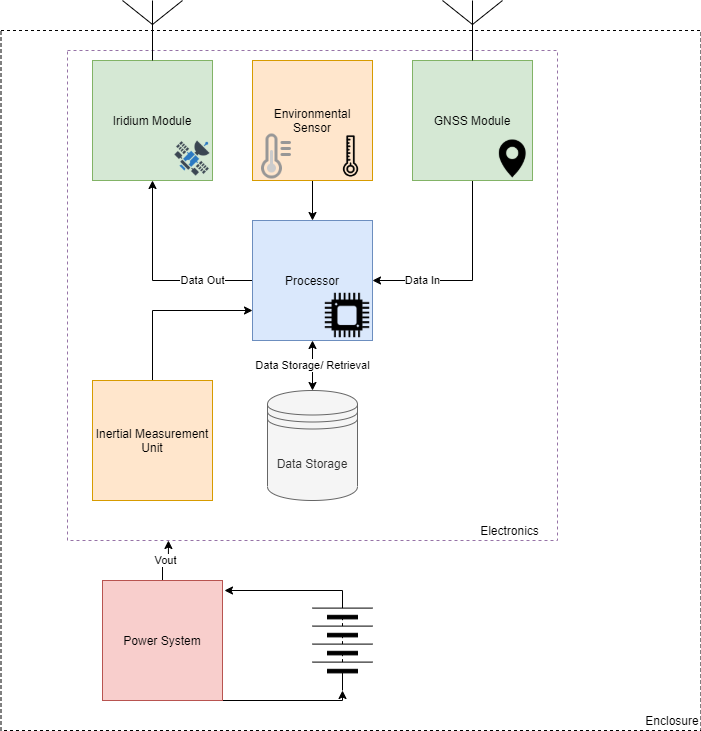
\includegraphics[width=\linewidth]{SHARC_NODE}
    \caption{Block diagram of the proposed autonomous system showing subsystem arrangement, data flow and interfaces with the environment.}
    \label{mbuoy}
\end{figure}

These subsystems can be further broken down into components requirements as shown in the figure below

\begin{figure}[H]
    \centering
    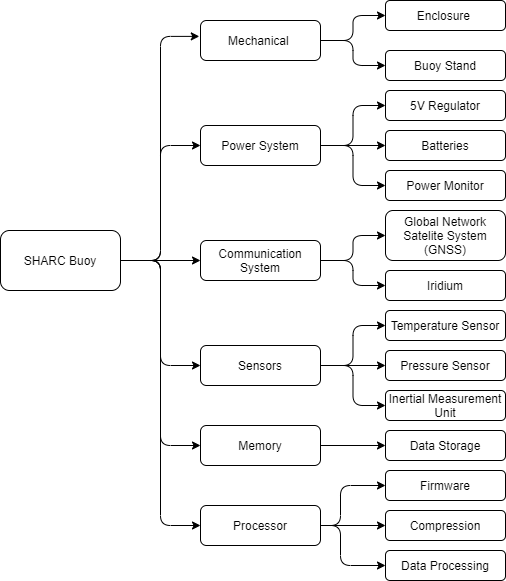
\includegraphics[width=0.8\textwidth]{Subsystem_Diagram.png}
    \caption{Breakdown of subsystems from table \ref{tab:subsys} into usable components.}
    \label{fig:ss_breakdown}
\end{figure}



\subsection{Technical specifications}

These technical specifications will be used to determine what hardware is required to construct the subsystems as showing in Figure \ref{mbuoy} above.

%%%FIX THIS TABLE

\begin{table}[H]
    \centering
    \caption{Technical specifications for the overall system}
     \setlength{\extrarowheight}{5pt}
    \resizebox{\textwidth}{!}{%
    \begin{tabular}{>{\centering\arraybackslash}m{0.25\textwidth}>{\raggedright\arraybackslash}m{0.6\textwidth} >{\raggedright\arraybackslash}m{0.35\textwidth} }
        \hline
         \textbf{Specification ID} & \textbf{Description} & \textbf{Functional requirement addressed} \\
         \hline
         \hline
         \multirow{2}{0.2\textwidth}{SP001} & \multirow{2}{0.6\textwidth}{Enclosure built using thermal resistant plastic.} & FR001\\ && FR002\\
         \hline
         \multirow{3}{0.2\textwidth}{SP002}  & \multirow{3}{0.6\textwidth}{Electronics to be mounted on a 1.5 m stand constructed from non-corrosive metal.} & FR002\\ && FR003\\ &&FR004\\
         \hline
         \multirow{1}{0.2\textwidth}{SP003} & System to include desiccant packets inside the enclosure. & FR003 \\
         \hline
         \multirow{1}{0.2\textwidth}{SP004} & Device to have a temperature operating range of $-40 ^\circ \text{ C to } 20 ^\circ$ C with $ 1^\circ$ C uncertainty. & FR009 \\
          \hline
         \multirow{1}{0.2\textwidth}{SP005}& Subsystems to be rated for $3.3 \textbf{ V to } 5$ V power. & FR008 \\
          \hline
         \multirow{1}{0.2\textwidth}{SP006}& Device shall survive for 1 month on a single set of cells & FR007 \\
          \hline
         \multirow{1}{0.2\textwidth}{SP007} & The device should cost less than R10,000 & FR016 \\
         \hline
         \multirow{1}{0.2\textwidth}{SP008} & System will contain flash chips for permanent storage. & FR012 \\
         \hline
         \multirow{1}{0.2\textwidth}{SP009}& System will use the STMicroelectronics STM32 series of microcontroller. & FR013 \\
         \hline 
         \multirow{1}{0.2\textwidth}{SP010} & The system shall be supplied by a regulated 5 V supply.  & FR014 \\
         \hline
         \multirow{1}{0.2\textwidth}{SP011} & The low power threshold occurs for voltages < 5 V & FR014 \\
         \hline 
         \multirow{4}{0.2\textwidth}{SP012}& Maximum current operations: & \multirow{4}{0.2\textwidth}{FR0014}\\
            &500 mA maximum start-up current. & \\
            &100 mA maximum active current. & \\
            &10 mA sleep current.& \\
         \hline
         \multirow{1}{0.2\textwidth}{SP013} & Device to be powered off or placed in sleep mode when inactive. & FR014 \\
         \hline
         \hline
    \end{tabular}}

    \label{tab:sys_specs}
\end{table}
\subsection{Acceptance test protocols}

In this section, the acceptance testing protocols for hardware and software modules is provided. These tests are designed to ensure that the devices meet the functional requirements outlined in table \ref{tab:hard_funcreqsl} to \ref{tab:elec_funcreqs}. A full description of the acceptance test protocols can be found in Appendix \ref{app:atp}. The goal of the acceptance criteria of each test as well as the the targeted module is given in table x below.

\begin{table}[H]
	\caption{A summary of acceptance test protocols from Appendix \ref{app:atp} showing the target and purpose of the test.}
	\label{tab:acceptance_test_summary}
	 \setlength{\extrarowheight}{5pt}
	\resizebox{\textwidth}{!}{%
		\begin{tabular}{cll}
			\hline
			\textbf{Acceptance test} & \textbf{Target} & \textbf{Purpose}\\
			\hline
			\hline
			AT001 	& Sensor modules. & Ensure module is online and functional \\
			\hline
			AT002	& All hardware modules.  & Test for faults and errors. \\
			\hline
			AT003 	& Device components. & Ensure selected components are rated for this application.\\
			\hline
			AT004	& Sensor peripheral libraries. & Verify software correctly interfaces with subsystem modules. \\
			\hline
			AT005	& Full system. & Ensuring an accelerated functional cycle meets the timing and sensing requirements. \\
			\hline
			AT006	& Sensor modules. & Calibrate the sensors against a known reference. \\
			\hline
			AT007	& Power subsystem. & Verify the power system meets the user requirements. \\
			\hline
			AT008	& Full system. & Ensure the device can operate in low temperatures. \\
			\hline
			AT009	&  Full system. & Ensure device functions in a remote environment. \\
			\hline
			\hline
		\end{tabular}
	}
\end{table}

%TODO create a summary of atp protocols as discussed with robyn

\section{Conclusion}

To summarise, this chapter outlines the design procedure for identifying critical subsystems and technical specifications to meet the user requirements. This will provide the basis for component and module selection which will be discussed in the next chapter.

\chapter{Platform design}
\label{sec:ch3_platform}

\section{Mechanical Features}

The mechanical design for the system falls outside the scope of this project however, it forms an integral part in protecting the electronics. The principle goal of the mechanically features are to anchor the device to the ice floe and protect it from the harsh environment. A buoy stand was designed by Keith Hutchinson with the University of Cape Town Workshop to satisfy this requirement. The stand is 1.2m tall with a base cross section of 0.71m and contains a cylindrical housing at the top where the device will be placed. A screw hole in the side of the stand allows the buoy to be fast-end to the stand to prevent it from falling out. The base of the stand is pyramid shaped with metal spikes to anchor the system to an ice floe. Due to the height of the stand, the system may be susceptible to tipping. This has been overcome by constructing the base to be heavier than the top thereby lowering the center of gravity. The stand was originally designed for the Trident buoys and this design has been modified by increasing the radius of the housing. 

\begin{figure}[H]
    \centering
    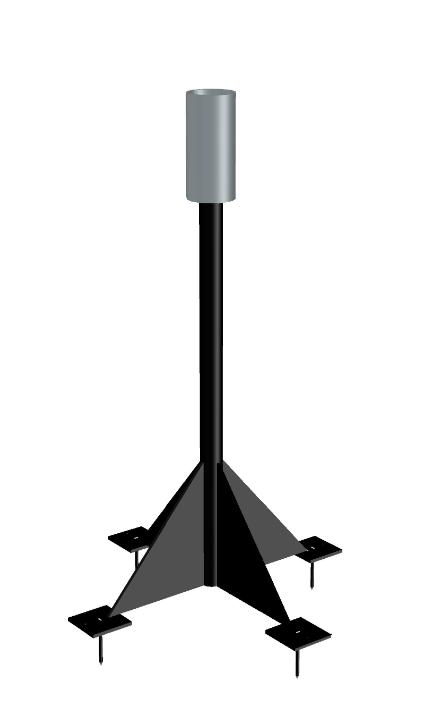
\includegraphics[scale = 0.7]{buoy_stand.PNG}
    \caption{3D Render of the buoy stand.}
    \label{fig:stand}
\end{figure}

The second part of the mechanical subsystem is the physical buoy enclosure. The greatest challenge for designing this system was selecting a material that was both lightweight and low-temperature resistant. A decision was made to use High-Density Polyethylene which has excellent low temperature thermal properties. The enclosure was designed to fit the housing on the buoy stand while providing ample room for the antennas of the various communication modules. the enclosure was split into 3 parts: A top enclosure, a bottom enclosure and a connector block. A schematic of the enclosure is shown in the figure below

\begin{figure}[H]
    \centering
    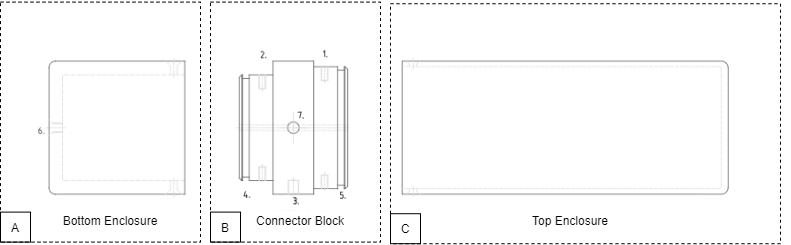
\includegraphics{enclo_schem.PNG}
    \caption{2-D Drawing of the Buoy Enclosure showing the separate components}
    \label{fig:enclo_schem}
\end{figure}

\begin{table}[H]
    \centering
    \caption{Primary Measurements of the buoy enclosure taken from the schematic in appendex \ref{fig:full_schem} \ref{fig:bot_schem} \ref{fig:top_schem} \ref{fig:conblock_schem}}
    \begin{tabular}{||l  l c||}
    \hline
         \textbf{Component} &   \textbf{Dimension} &   \textbf{Value (mm)} \\
         \hline
         \hline
         \multirow{4}{*}{Top Enclosure} & height & 240\\
         &  diameter & 98  \\
         &  wall thickness & 4 \\ 
         & base thickness & 5 \\
         \hline
        \multirow{3}{*}{Bottom Enclosure} & height & 100\\
         &  diameter & 98  \\
         & thickness & 10 \\ 
         \hline
        \multirow{5}{*}{Bottom Enclosure} & height & 80\\
         &  outer diameter & 98  \\
         &  top inner diameter & 89.94  \\ 
         &  bottom inner diameter & 77.85\\
         &  O-ring Thickness & 2.6 \\
         \hline
    \end{tabular}

    \label{tab:enc_meas}
\end{table}

This design allows for easy access to the electronics as well as separation between the various subsystems. The connector block acts as a connection point for the electronics in version 1. This point of contact was a 3d printed connector for a vertically mounted PCB. In version 2, this was replaced by a row of screw holes around the connector block to connect a horizontal Stack of customised PCBs. This was found to greatly improve the robustness of the system and prevented components from breaking. The communication modules, microcontroller and sensors were mounted in the top enclosure while the batteries and power system were placed in the bottom enclosure. The power system was connected to the top enclosure through a drill hole in the connector block. The system was waterproofed by placing 2 o-rings on either side of the connector block. The top and bottom enclosure are fastened to the connector block using a a flat head counter sunk hex screw. Finally a drill hole in the connector block allowed the system to be secured to the buoy stand preventing it from falling out during deployment.

\section{Electronics}

The electronics for the system refer to the Communication subsystems, power electronics, sensors and processors. Due to project time constraints, the approach to developing the platform was to select off the shelf components that satisfied the requirements shown in table \ref{tab:sys_specs}. Further consideration was given to components that were low power (SP011, SP012) and cost effective components (SP013). Additionally, devices with intelligent operations were selected as this would allow us to effectively control the current consumption and operations of the device. These consisted of components with programmable settings such as digital sensors, actuators and modems. The following section gives an overview of the selection consideration for each subsystem

\subsection{GPS}

A Ublox Neo-7m was initially selected as it was easy to procure and has a small form factor. The module comes on a Waveshare breakout board which significantly decreases the development time. The board comes with an active patch antenna which has a gain of about 30dB. In addition, the component is low power with a relatively fast acquisition time and accuracy. The device also can be configured to output diagnostic information and Dilation of procession with the associated measurement which can provide a greater understanding of satelite connectivity in the region. However, by the time we requested more modules, the device was out of stock and had depreciated. To overcome this, we opted for the Neo-M9N module which had significantly improved performance at a higher cost. The table below shows a comparison of the two modules and their key performance parameters.

\begin{table}[H]
    \centering
    \caption{Comparison of key parameters between the initial Ublox Neo-7m gnss module and the updated Ublox Neo-N9M module}
    \begin{tabular}{|l |l |l|}
    \hline
        \textbf{Description} & Neo-7M & Neo-M9N\\
        \hline
         Positional Accuracy: & 2.5m  & 2.0m\\
         Communication Type: & UART, I2C, SPI & UART, I2C, SPI\\
         Cold-Start Time:& 30s & 26s\\
         Supply Voltage & 1.65V - 3.6V & 2.7V -3.6V\\
         Active Current Draw & 32mA &  42mA\\
         Price & R269 \footnotemark & R1,195.45 \footnotemark\\
         \hline
    \end{tabular}
    \label{tab:neo7}
\end{table}
\footnotetext[1]{from Digikey \url{https://www.digikey.co.za/} ordered on 09/2020} 
\footnotetext{from Microrobotics \url{https://www.robotics.org.za/} ordered on 19/12/2018}
The Neo 9-m offers improved performance at a higher cost and higher power consumption. This module comes on a Sparkfun breakout board with an option for an external u.fl antenna or an integrated chip antenna. The chip antenna however has a very small gain making it unsuitable to be used for this application. Therefore, an additional antenna was bought.

\subsection{Iridium}

The Iridium modem is critical for ensuring data can be transmitted from remote locations. When selecting a modem, key considerations were given to the physical size, Bandwidth as well as coverage. In addition, we require a module that is low powered and cost effective. For this reason, we have selected the Rock block 9603 modem which has the following key specifications. This is a module that contains an Iridium 9603 modem on a specially -designed power board. The device communicates via UART with the option for flow control. The module contains a 10-pin picoblade. The module contains 4 communications pins, 1 digital input pin and 2 digital output pins for interfacing with. Power is supplied either through a 5V pin or 3.3V pin in addition to the ground pin. A brief description of the pin out is given in the table below: 

\begin{table}[H]
    \centering
    \caption{Pinout for the Rockblock 9603 Iridium Modem}
    \begin{tabular}{c l l}
        \hline
         Pin Number: & Label & Pin Description\\
          \hline
          \hline
         1 & RXD & UART Output Pin \\
        
         2 & CTS & Flow Control Clear To Send\\
         3 & RTS & Flow Control Request To Send\\
         4 & NetAv & Network Available \\
         5 & RI & Ring Inidcator \\
         6 & TXD & UART Input Pin \\
         7 & OnOff & Sleep Control\\
         8 & 5V & 5V max supply pin \\
         9 & Li-Ion & 3.7V max supply pin \\
         10 & GND & Ground \\
         \hline
         \hline
    \end{tabular}

    \label{tab:ir_pinout}
\end{table}

The device communicates via UART through the RXD and TXD pins. The CTS and RTS pins are optional if flow control is required. The OnOff pin can be used to put the device to sleep which significantly improves power performances. Finally, The NetAv and Ring Indicator are notification pins that can be used to indicate whether there is sufficient signal to transmit as well as to notify when a message is waiting to be downloaded respectively. 

Finally, the key characteristics for the device are shown in the table below:

\begin{table}[H]
    \centering
    \caption{Table showing key parameters and performance characteristics taken from the datasheet}
    \begin{tabular}{|c|c|}
        \multicolumn{2}{l}{Mechanical Features:}\\
        \hline
        \textbf{Antenna: } & Patch or External SMA\\
        \hline
        \textbf{Temperature Rating:} & -40ºC to +85ºC\\
        \hline
       \textbf{Dimensions}  & $45.0 \times 45.0 \times 15.0$ mm  \\
       \hline
        \textbf{Cost: } & R2,850.56\\
               \hline
       \multicolumn{2}{l}{Power Characteristics:}\\
       \hline
       \textbf{Supply Voltage} & 5v or 3.7v Li-Ion \\
       \hline
       \textbf{Start-Up Current} & 450mA \\
       \hline
       \textbf{Active Current} & 100mA \\
       \hline
       \textbf{Sleep Current} & 200uA\\
       \hline
        \multicolumn{2}{l}{Communication:}\\
        \hline
         \textbf{Baudrate} & 19200 b/s \\
        \hline
         \textbf{ Data bits} &  8\\
        \hline
         \textbf{Stop bits} & 1 \\
        \hline
         \textbf{Parity} & none \\
        \hline
        \textbf{Max Upload size} & 340 bytes \\
        \hline
        \textbf{Max Download Size} & 270 bytes \\
        \hline
    \end{tabular}

    \label{tab:ir_specs}
\end{table}

\subsection{Sensors}

2 versions of the buoy were developed from 2019 - 2020 with different sensing capabilities. The first version consisted of a DS18B20 Temperature sensor. This was a low cost, small form factor device that interfaced over One-wire. In version two, this was dropped in favour of the Bosh Sensortech BMP280 sensor. The BMP featured improved sensing capabilities, temperature compensation as well as a programmable interface. In addition, the sensor contains both an ambient temperature sensor as well as a pressure sensor. A comparison of each device is given in the table below

\begin{table}[H]
    \centering
    \caption{Comparison of performance between the BMP280 and DS18B20 environmental sensors.}
    \begin{tabular}{|c|c|c|}
    \hline
         & \textbf{BMP280} & \textbf{DS18B20} \\
         \hline
         Temperature Range & $-40^\circ C \text{ to } 85^\circ C$&$-55^\circ C \text{ to } 125^\circ C$ \\
         \hline
         Accuracy & $1^\circ C \text{ for } T < 0^\circ C$ & $1^\circ C \text{ for } T < 0^\circ C$ \\
         \hline
         Pressure Range  & N/A & 300 to 1100 HPa \\
         \hline
         Pressure Accuracy & N/A & 1.7 HPa $ \text{ for } T < 0^\circ $\\
         \hline
         Price & R87,84 & R85.17 \\
         \hline
    \end{tabular}
    \label{tab:senv_spec}
\end{table}

The BMP 280 is a chip that can be ordered standalone or comes on a I2c/SPI ready breakout board. The device on a breakout board is cheaper than than DS18B20 and can measure both temperature and Pressure whereas the DS18B20 can only measure temperature. The Power characteristics of each device are given in the table below

\begin{table}[H]
    \centering
    \caption{Comparison between supply voltage and current draw of the BMP280 and DS18B20}
    \begin{tabular}{|c|c|c|}
        \hline
         &  \textbf{BMP280} & \textbf{DS18B20}\\
         \hline
         Supply Voltage & 3.0V - 5.5V & 1.71V - 3.6V\\
        Sleep Current & $0.75\mu A$ & $0.3\mu A$\\ 
        Active Current & $1500\mu A $ & $4.2\mu A$\\
        \hline
    \end{tabular}

    \label{tab:env_power}
\end{table}

The BMP280 was chosen for its comparable performance and accuracy. In addition, the BMP280 features more sensing capabilities and is more power efficient and cost effective than the DS18B20 making it suitable for this application.\par 

Finally, a digital sensor for power monitoring was selected to provide constant feedback on the status of the power system. This will be used to monitor the battery voltage as well as the current draw to make sure that the system does not deplete the energy reserves to quickly. To achieve this a INA219A IC was selected and mounted on a custom PCB with a shunt resistor of known resistance. The device has a high reported accuracy of 1\% over a full temperature range and is fully programmable. The device  communicates via I2C with 16-bit registers storing ADC values for  Current (mA),Voltage (V) as well as power (mW). The device is extremely low power with a high voltage measurement range and on-board calibration features. Some key performance parameters are shown in the table below:

\begin{table}[H]
    \centering
    \caption{Performance specifications for the INA219 current monitor chip.}
    \begin{tabular}{|l|l|}
    \hline
         \textbf{Operating Temperature: }& $-40\degree C\text{ to } 125\degree C$ \\
         \hline
         \textbf{$V_{shunt}$ range: }& $40mV \text{ to } 320mV$\\ 
         \hline
         \textbf{$V_{bus}$ rage: } & $0V - 16V \text{ or } 0V-32V$\\
         \hline
         \textbf{ADC Resolution: } & 12-bits\\
         \hline
         \textbf{Measurement Error: } &$\pm 1\%$\\ 
         \hline
         \textbf{Price: } & R17.77\footnotemark\\
         \hline
         \multicolumn{2}{l}{Power Characteristics}\\
         \hline
         \textbf{Supply Voltage: } & $3.3V \text{ to } 5V$\\
         \hline
         \textbf{Quiescent Current: } & $0.7mA \text{ to } 1mA$\\
         \hline
         \textbf{Standby Current: } & $6\mu A \text{ to } 15\mu A$\\
         \hline
    \end{tabular}

    \label{tab:INA_spec}
\end{table}
\footnotetext{source: \url{https://www.digikey.co.za/}}

\subsection{Inertial Measurement Unit}

The MPU6050 is a 6-axis IMU that measures the acceleration and rotational velocity of 3 axes respectively.This component has a small form factor, low power and is fully programmable allowing the device to operate in different modes thereby optimising the data flow to and from the device. While the device does not contain a magnetometer, this is not an issue since the region suffers greatly from magnetic distortion \cite{kohout2015device} thereby rendering all readings to be unreliable. In addition, The acceleration of waves can be defined by the stoke supper limit \cite{kohout2015device} as 0.5g for a non breaking wave. The device has a programmable full scale range for both the accelerometer and gyroscope. IT contains an IIR filter and on-board self testing for added robustness and data integrity thereby making it  the ideal device for this application. The key parameters for the device are shown in the table below:
\begin{table}[H]
    \centering
    \caption{Performance Characteristics of the MPU6050 6-axis IMU }
    \begin{tabular}{|l|l|}
    \multicolumn{2}{l}{Accelerometer:}\\
    \hline
       Full Scale Resolution:  & $ \pm 2g \text{ to } \pm8g$\\
       \hline
        Sensitivity: &  $61.17 \mu g/LSB^{-1} \text{ to } 488.281\mu g/LSB^{-1}$\\
         \hline
        Sample Rate: & 4Hz - 1000Hz\\
         \hline
        Noise Performance: & $400\mu g/\sqrt{Hz}$\\
         \hline
         \multicolumn{2}{l}{Gyroscope:}\\
         \hline
           Full Scale Resolution:  & $\pm 250\degree/s \text{ to } \pm 2000\degree/s $ \\
       \hline
        Sensitivity: &  $7.63(\mu\degree/s)/LSB^{-1} \text{ to } 60.98(\mu\degree/s)/LSB^{-1}$\\
         \hline
        Sample Rate: & 4Hz - 8000Hz\\
         \hline
        Noise Performance: & $0.005(\mu\degree/s)/\sqrt{Hz}$\\
         \hline
         \multicolumn{2}{l}{Device Characteristics:}\\
         \hline
         Temperature Range: & $40\degree C \text{ to } 85 \degree C$\\
         \hline
         Low Pass Filter Range: & 5Hz to 256Hz \\
         \hline
         Supply Voltage: & 2.375V to 3.46V\\
         \hline 
         Active Current: & 3.9mA (Max) \\
         \hline
         Low Power Current: & $< 20 \mu A$ for $ODR < 5Hz$\\
         \hline
         Cost: & R40.00 \footnotemark\\
         \hline
    \end{tabular}
    \label{tab:mpu_specs}
\end{table}
\footnotetext{Source: \url{https://www.communica.co.za/}}

The device has a high range for both gyroscope and imu with ideal low power performances making it the ideal device. In addition, the device comes prototype ready on the GY-521 development board. The device can be interfaced either using SPI or I2C. For this application, the device was interfaced with using I2C.

\subsection{Memory}

Physical memory is an important feature in the device as it allows for permanent storage of data during the life cycle of buoy. Having the device in various sleep modes may result in lost data if the data is stored in RAM.

Flash Chips were selected as a permanent Solution. An array of 4 AT45DB641E SPI Serial Flash Chips were selected and mounted on a PCB directly interfacing with the system. Each chip can hold up to 64Mbit of data. Data can be read/ written at speeds of up to 85MHz of 15MHz in low power mode. The device is low power with high data retention requiring a supply voltage of 1.7V – 3.6V and draws a maximum of 11mA in Active Read mode thereby making it one of the lowest power consumption components in the system. In addition, the device comes with 2 x 256byte buffers that can store data while a read/ write operation is taking place. Memory is Organized into sectors (2 – 256 Kbs long), blocks (2kB long) and pages (256 bytes) with write, read and erase options at each level. The following table shows key performance characteristics

\begin{table}[H]
    \centering
    \caption{Key performance characteristics for the AT45DB641E flash chips.}
    \begin{tabular}{|l|l|}
    \hline
    Operating Temperature:  & $ -40\degree \text{ to }85 \degree$ \\
    \hline
    Storage Capacity: & 64 Mbit \\
    \hline
    Supply Voltage    & 1.7V -3.6V\\
    \hline
     Standby Current: & $45\mu A$ \\
     \hline
     Active Current:  & $22mA$ \\
     \hline
     Unit Cost:       & R 65.307 \footnotemark\\
     \hline
    \end{tabular}
    
    \label{tab:flash_specs}
\end{table}
\footnotetext{Source: \url{https://za.rs-online.com/}}
\subsection{Processor}

For the processor, a single processing unit was selected to reduce complexity of the system. However, in order to satisfy the requirements for the buoy, a processor must be selected with sufficient peripheral ports to handle communication from all sensors, communication modules and memory banks. In addition, there should be sufficient digital input and output pins to control the sensors and provide feedback The communication peripheral requirements are condensed into the following table: 

\begin{table}[H]
    \centering
    \caption{ Type and number of communication ports in order to facilitate communication with  all the external modules.}
    \begin{tabular}{|l|l|}
        \hline \hline
        Peripheral Name: & Qty \\
        \hline \hline
        UART & 2\\
        I2C & 2\\
        SPI & 2\\
        Digital Pins & 11\\
        \hline 
    \end{tabular}
    \label{tab:micro_ports}
\end{table}

Additionally, the processor needs to have a high resolution and large memory bank to handle incoming data. For this reason, a 32-bit micro-controller was identified as the ideal component for the processing system. 3 processors were selected from the STM32 range of microcontrollers and prototyped at various phases during the development cycle. The first version of the buoy contained the STM32F407 which is available on a 100-pin development board thereby decreasing the development time and increasing the technology readyness level of the system. This device was found to have more peripherals than required and had a large power requirement. Therefore the device was replaced by the STM32F446-RE which had significantly reduced peripherals and more optimal performance. The final processor selected was the STM32l476RG. Which matched the STM32F446 in pinout and peripheral however it was significantly more optimised for low power operation. The device had significantly more wake up pins with an extremely low power consumption therefore being the optimal choice. In addition, the development board for the STM32l476 has an on-board debugger which can be removed to reduce the physical size of the device. The STM32L4 can also be configured to passively detect a brownout event as well as a low power event which provides critical feedback regarding the device's performance. Some key performance parameters of the STM32l476 are shown in the table below:
 
 \begin{table}[H]
     \centering
     \caption{Performance parameters for the STM32L4 microcontroller. }
     \begin{tabular}{|l | l|}
     \multicolumn{2}{l}{Electrical Characteristics:}\\
     \hline
      \textbf{Input Voltage: }    & $1.71V \text{ to } 3.6V$ \\
      \hline
      \textbf{Active Current Draw: }    & $100 \mu A/Hz$ \\
      \hline
      \textbf{Shutdown Mode Current Draw: }    &  $30nA$ \\
      \hline
      \textbf{Standby Mode Current Draw: }    &  $420nA$ \\
      \hline
      \textbf{$V_{brownout}$ Threshold:} &  $1.66V \text{ to } 2.90V$\\
      \hline
       \multicolumn{2}{l}{Computational Characteristics:}\\
     \hline
     \textbf{Processor: }    &  ARM Cortex-M4 \\
     \hline
     \textbf{MCU Size: }     & 32-bit\\
     \hline
     \textbf{Float representation: } & Hardware FPU \\
     \hline
     \textbf{Flash size: } & 1MB\\
     \hline
     \textbf{RAM Size:} & 128 KB\\
     \hline
     \textbf{Clock Source: } & LSE, HSE, LSI, MSI, HSI \\
     \hline
     \textbf{System Clock Frequency: } & 4MHz to 80MHz \\
     \hline
     \textbf{Dhrystone Benchmark: } & 1.25 DMIPS/Hz \\
     \hline
     \multicolumn{2}{l}{Communication Ports:} \\
     \hline
     \textbf{Total  Communication ports: } & 20 \\
     \hline
     \textbf{UART Ports} & 5 \\
     \hline
     \textbf{I2C Ports} & 3 \\
     \hline
     \textbf{SPI Ports} & 3 \\
     \hline
     \end{tabular}

     \label{tab:stm_spec}
 \end{table}
 
 The STM32l4 also features seven general purpose timers as well as two advanced timers and two low power timers. In addition, the device has five wake up pins which allow the device to be woken up from deep sleep (shutdown) via an external source. The device is capable of DSP processing using external libraries provided by the manufacturer and a real-time clock thereby making it the ideal component to be a processor for the buoy.
 
 \subsection{Power Electronics}
 
 Based on the aforementioned Hardware selection, the following power requirements are outlined in the table below:
 
 \begin{table}[H]
     \centering
      \caption{Current consumption of various components as well as the estimated maximum possible current draw}
     \begin{tabular}{|c|c |c|c|}
         \hline
         Device Name & QTY &  Supply Voltage & Maximum current Draw\\
         \hline
         Ublox NEO-M9N & 1 & 3.3V & 42mA \\
         \hline
         Rockblock 9603 & 1 & 5V &  450mA\\
         \hline
         BMP280 & 1 & 3.3V & 0.0042mA\\
         \hline
         INA219A & 1 & $V_{Bat}$ & 1mA\\
         MPU6050 & 1 & 3.3V & 3.9mA\\
         \hline 
         AT45DB641E & 4 & 3.3V & 88mA\\
         \hline
         STM32L476RG & 1 & 5V & 2.6mA\\
         \hline
         \cline{4-4}
         \multicolumn{2}{c}{} &\multicolumn{1}{c}{\textbf{total:}} & \multicolumn{1}{c}{587.50mA} \\
         \cline{4-4}
         \cline{4-4}
     \end{tabular}

     \label{tab:pow_budget}
 \end{table}
 
 From table \ref{tab:pow_budget} we can expect a maximum current draw of 587.50. The largest consumer of power is the Rock-block 9603 which can draw up to 450mA when charging. Therefore, the power supply needs to be able to supply at-least 500mA during start up. Current can be conserved by placing the devices into sleep mode which further reduces the current consumption from the batteries. Finally, By only turning the components on when required, even less power can be conserved. \par 
 
 Therefore, a regulator is required that is capable of supplying the required current  while being able to stand the drastic changes in current consumption. A decision was made to use a 5V low Dropout regulator to supply the 5V components directly i.e. the iridium modem and the micro-controller. The 3.3V components are powered through the on-board 3.3V regulator for the STM32L4 nucleo development board. The Low Dropout regulator is a LP3876 7V LDO capable of supplying up to 3A. The device has a quick response to step changes and an adjustable output voltage thereby making it the ideal device to supply power. The output voltage level can be controlled by selecting capacitors. For this application a $10 \mu C$ tantalum capacitor was used as tantalum capacitors have  excellent robustness and transient responses especially at low temperatures.  Some key characteristics for the device are given in the table below
 
 \begin{table}[H]
     \centering
      \caption{Key Performance Characteristics for the LP3876 Low Dropout Regulator}
     \begin{tabular}{|l|c|}
     \hline
          Input Voltage & $2.5V \text{ to } 7.0V$  \\
          \hline
          Voltage Regulation (over current)& 0.14\%\\
          \hline
          Dropout Voltage at 3A & 0.8V to 1.2V  \\
          \hline
          Quiescent Current at 3A &  14mA\\
          \hline
          Temperature Range & $-40 \degree C \text{ to }125 \degree C$\\
          \hline
          Unit Cost & R95.19 \footnotemark\\
          \hline
     \end{tabular}    
     \label{tab:lp_spec}
 \end{table}
 
 \footnotetext{source: \url{https://www.digikey.co.za/}}
 
The LDO was placed on a customised PCB  with the INA 219 Current sensor as well as an indicator LED to show that the batteries have sufficient charge. The power board was supplied by 3.6V C-cell LiSOCl2 batteries. These batteries have ideal low temperature characteristics as well as a high capacity. 2 cells were placed in series to create a 7.2V power source which was placed in parallel with another 7.2V array to increase the capacity. The batteries, battery holders and power board are connected to form a single subsystem which was placed in the bottom enclosure and connected to the micro-controller via a 7-pin cable.

\section{Final Assembly}
\label{sec:ch3_final_assembly}
The final electronics choice and configurations are shown in the figure below:

\begin{landscape}\centering
\vspace*{\fill}
\begin{figure}[htpb]
  \centering
  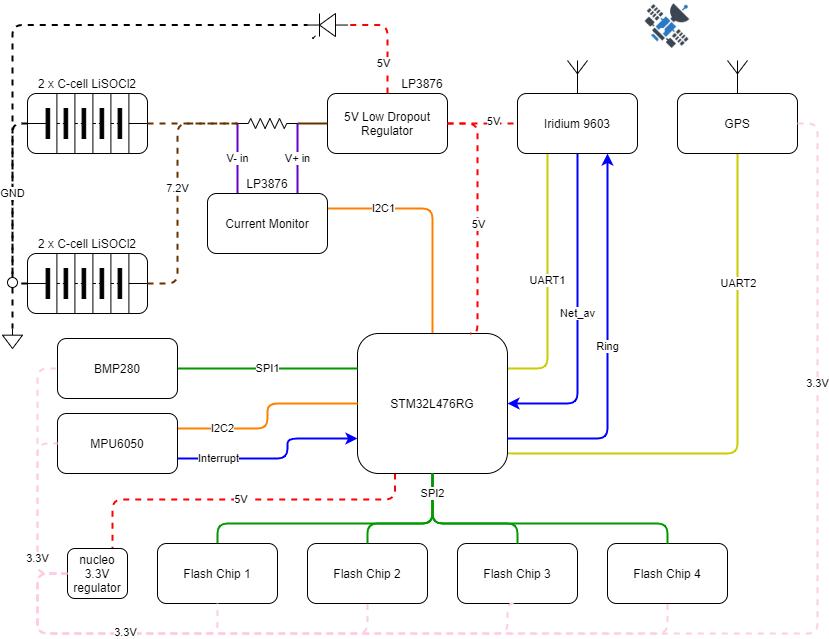
\includegraphics[height=0.6\textheight, width=1.2\textwidth]{figs/SHARC_Final.png}
  \caption{Simplified schematic of the final version of SHARC buoy showing power supply (dash), communication (solid) and digital connections (arrows) and configurations}
    \label{fig:sharc_final}
\end{figure}
\vfill
\end{landscape}


A final costing of the system is provided in the table below:
\begin{table}[H]
    \centering
    \caption{Approximate procurement cost for a single SHARC buoy node.}
    \begin{tabular}{l c r r}
    \hline \hline
        \textbf{Component Name:} & \textbf{QTY:} & \textbf{Unit Cost} & \textbf{Total:}  \\
        \hline \hline
        Buoy Enclosure and Stand  & 1 & R1,206.84 & R1,206.84 \\
        Ublox Neo-M9N & 1 &  R1,195.45 &R1,195.45\\
        Rockblock 9603 & 1 & R3,278.144 & R3,278.144 \\
        M1621HCT Helical Antenna & 1 & R1,411.15 & R1,411.15 \\
        BMP280 & 1 & R46.00 & R46.00 \\
        INA219A & 1 & R17.77 & R17.77 \\
        MPU6050 & 1 & R40.00 & R40.00 \\
        AT45DB641E & 4 & R65.307 & R261.229 \\
        Nucleo-l476RG & 1 & R215.98 & R215.98 \\
        Fanso C-cell 9000mAh Battery & 4 & R101.81 & R407.24 \\
        BHC-2ND Battery Holder & 4 & R61.87 & R247,48 \\
        LP3876 5V regulator & 1 & R95.19 & R95.19 \\
        Wiring and Connectors & - & R136.46 & R136.46 \\
        \hline 
        \hline
        & & \textbf{ Grand Total: } & R8,421.13\\ 
        \hline \hline
    \end{tabular}
    \label{tab:total_cost}
\end{table}

Customised PCBs were designed to connect the various subsystems together. The device was kept modular by separating PCBs and grouping devices by functionality. A circuit board was created for the Dropout regulator and INA219 current sensor which was affixed to 4 x C-cell battery holders.The battery holders have leads which were were arranged in a 2-series, 2- parallel configuration.

\begin{figure}[H]
    \centering
    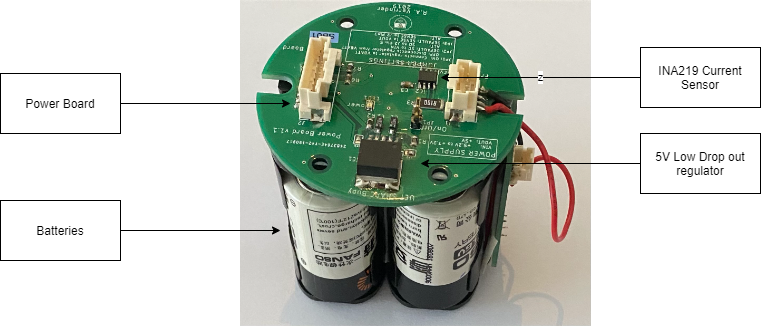
\includegraphics[scale = 0.5]{bot_encl.png}
    \caption{Power Module for the SHARC BUOY. A custom PCB with Dropout Regulator and current sensor connected to a battery pack}
    \label{fig:bot_elec}
\end{figure}

This module was placed in the bottom enclosure and fastened to the connector block using a hex screw. A customised 7-pin duraclick cable connects the module to the modules in the top enclosure. A main connector board was developed with duraclick connections for each of the aforementioned devices. The board contains 2  2x16 female header rows to fit the morpho connectors of the nucleo-l4 development board. 2 more disc-shaped PCBs were developed. First a communication boards which contains a 4-pin female header to connect the ublox GPS module and 2 brackets to mount the iridium module vertically. A helical antenna connects to an SMA antenna on the Iridium module. Then a sensor board for the IMU and environmental sensor. The boards were connected in a stack configuration and fastened to the connector block using M6 metal Hex Spaces with the communication board being placed at the top for direct line of sight with satellites. The environmental board was secured to the base of the connector block with the BMP280 placed face-down over a hole drilled through the connector block allowing it to interface with the environment.
 \begin{figure}[H]
     \centering
     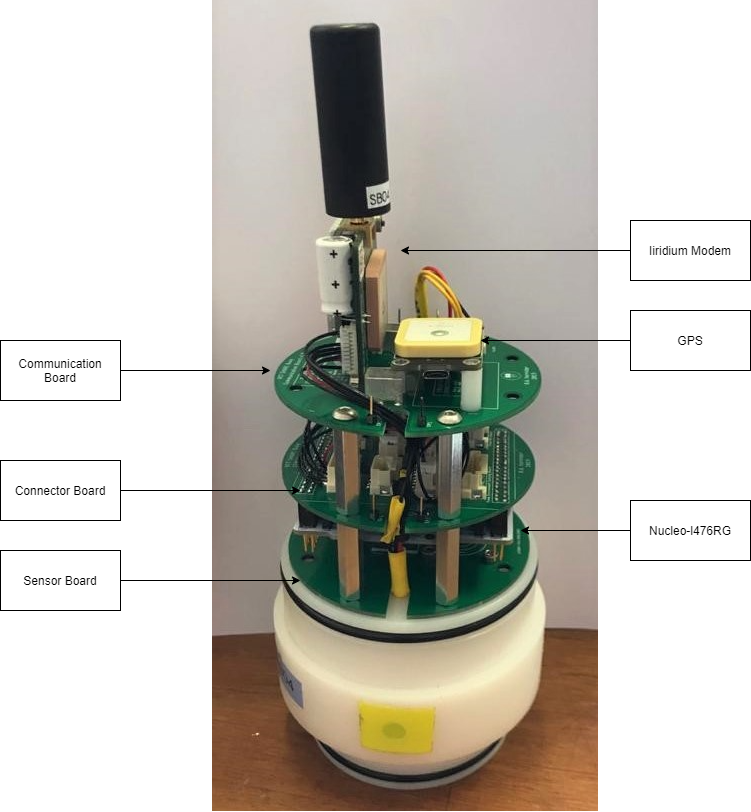
\includegraphics[scale =0.5]{Top_encl.png}
     \caption{Electronic Stack for the top module consisting of connector board, micro-controller board and sensor board attached to the connector block }
     \label{fig:top_elec}
 \end{figure}

This configuration greatly increases the robustness of the electronics and can overcome breaking caused by poor handling or improper deployment.  The top enclosure is placed over the electronics and fastened to the connector block using Hex screws. Finally, the system is placed in the stand housing and secured using another hex screw.

\begin{figure}[H]
    \centering
    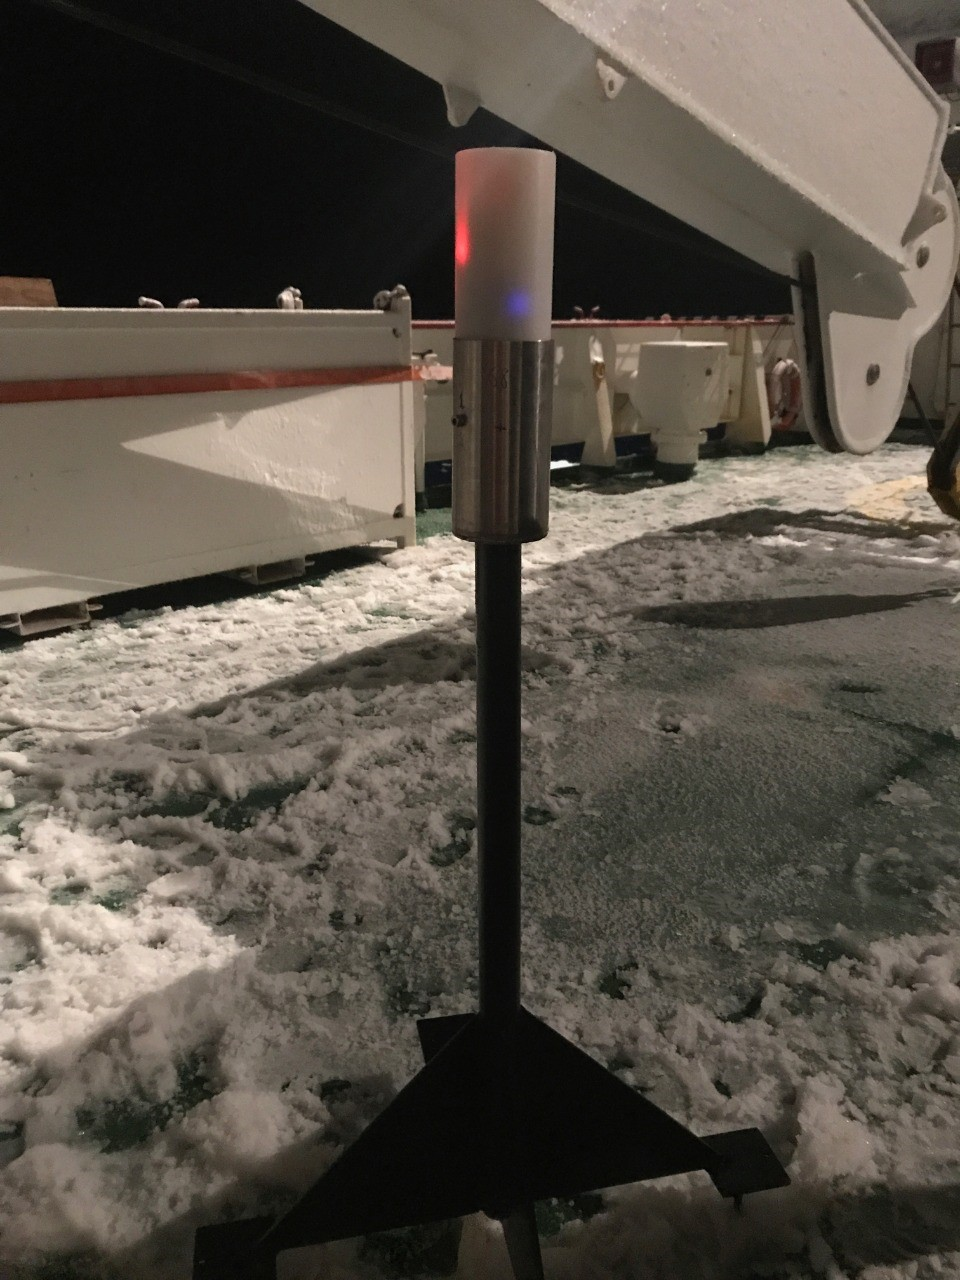
\includegraphics[scale = 0.5]{full buoy.jpg}
    \caption{SHARC BUOY fully assembled and in deployment state. Electronics placed in enclosure and fastened to the buoy stand. LEDs on the various components indicate that the device is in working order}
    \label{fig:my_label}
\end{figure}

\chapter{Software Design}
\label{sec:ch3_soft}
This section outlines the design methodology for the SHARC Buoy Software. The software cycle was designed with consideration towards the IEEE software standard 12207.1\footnotetext{Software life cycle processes—Life cycle data\cite{IEE_STD_SOFTCYCLE}}.


The software structure was kept as compartmentalised as possible to improve the modulator of the firmware. This would allow for fewer changes to be made during the design process allowing for a quick response to hardware changes. The design process was iterative as changes were made over the design cycle to the micro-controller platform as well as the sensors. In addition, some of the required libraries had depreciated and needed to be replaced.  This section will focus solely on the firmware design for the overall system as well as the subsystem. 

This section begins with an overview of the development environment which discusses the tools, platform and any libraries that were used. Then an overview of the main firmware is given. Each aspect of the system is described in terms of function, configuration parameters as well as location in the overall scope.

\section{Software Architecture}

The STM32 series does not come loaded with any Operating System. Therefore, firmware development had to occur on bare metal. In addition, the firmware had to be tailored to the specific micro-controllers architecture. The Atollic Truestudio IDE allowed for development to take place in C. The program comes packaged with an ARM development tool chain and a C compiler allowing for code to be compiled and flashed onto the board via a USB cable. The manufacturer also provides a set of driver files and  initialisation tools. The project was written in C which allowed for higher-level code to implemented while still optimising for size and speed on the device. In addition, C allows for the program to include drivers and resources from the manufacturer. \par 

The Firmware was designed using a top down approach. The overall system was decomposed into 3 distinct layers as shown in the figure below

\begin{figure}[H]
    \centering
    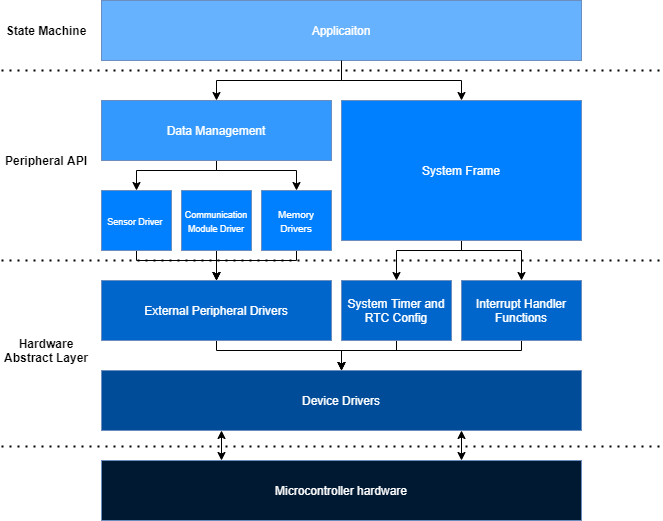
\includegraphics[width= 0.7\linewidth]{soft_arch.png}
    \caption{Diagram showing the decomposition of the overall firmware into distinct layers and the relationship between each part.}
    \label{fig:soft_arch}
\end{figure}

The Hardware Abstract layer consists of the driver files used to initialise and control the hardware of the micro-controller.This layer is platform specific therefore needs to be tailored to the architecture of the micro-controller. The manufacturer provides hardware driver files which were used to form the Hardware abstract Layer.The Standard Peripheral Library (SPL) was used in the first version of the firmware however, the library had depreciated and was replaced with the Hardware Abstract Layer (HAL) libraries. HAL libraries were used to form the foundation of the code as it allows for the code functionality to run independently from the hardware architecture. Should a new micro-controller be required, the HAL library simply needs to replaced. Therefore allowing the firmware to maintain modularity and increase portability. In addition, the HAL Library offers robust error checking and flagging. If a peripheral fails at any point during run time, the libraries provide handlers and flag signalling to handler the error. \par 
Once The HAL Layer was finished, customised driver files were written for each module. These files were written to interface with the sensor through the HAL layer thereby reducing dependencies on the hardware, in addition, these driver files were created to abstract the initialisation and configuration process of each peripheral as well as the hardware routines that occur. In addition, some external modules required the use of more than one peripheral such as timer channels for input capture or GPIO pins for External interrupt detection. Finally, these drivers are critical for managing the flow of data too and from the module. The files contain functions that interpret incoming data bytes and convert them to the relevant data type.

\par 

Finally, driver files, configuration files and other libraries are synthesised and sequenced into one main program. This program calls the functions defined in the Driver files. This program provides a frame for the various modules to interact with system. This will be discussed in greater detail in the section below

\section{Project Structure}

The project was set up using CUBEMX for creating peripheral initialization and handling functions. Final code for the project can be found in the folder BUOY\_Frame\_L4. All the tools, definitions and functions developed for the Buoy frame have been organised into the library files Sharc\_Frame.h and Sharc\_Frame.c. This allows for the frame to ported over multiple projects allowing for a new firmware version to be developed from scratch instantly.
The project code files are organised into the following folders:

\begin{enumerate}
    \item Drivers
    \item src
    \item Start Up
\end{enumerate}
The project code files are organised into the following folders:
1.	Drivers 
2.	SRC
3.	Start Up
The Drivers folder contains the HAL and CMSIS libraries for the device.  The SRC Folder contains the main.c file which acts as the entry point for the program to run. The start up file contains assembly code that specifies the vector table, Hard fault/ Reset Handler Entry Points as well as the entry point for the main code. When the file startup\_stm32l476xx.s is run, the program enters into the main() function and begins running from there. The SRC folder contains the .h/.c pair Sharc\_Frame files which are implemented in the main.c 
The main() code consists of a set up phase and a loop phase. During the set-up, the functions HAL\_Init(); and SystemClock\_Config(); are used to reset the peripherals and the systick timer and set the System clock to the correct source and speed. These two functions run in the set-up phase of the code and are called whenever the program re-enters the main function. The next step in the set up phase is to configure the unused GPIO pins to analog floating mode. This greatly reduces the current consumption by the micro controller. The peripherals required for debugging the code are placed here. Before deployment, the code will be removed. This phase is referred to in the program as the System Init and Clock Configuration. It is the first phase to be run.
The next phase in the Set-up is the Power and Reset State Check. If any power event occurs, a software reset is generated, and the program will restart from the main() function. When this happens, a flag is set in the RCC\_CSR. This can occur in the form of a brown out, Pin reset or Low Power event. This phase will check for the occurrence of any event and handle them before the program enters the main loop. Finally, if successful the program will enter the main loop and the firmware will begin.  

\subsection{Power Mode Selection}

 The focus on development optimizing for power consumption as well as accuracy. The system requirements are extremely flexible since the required sampling rate is very slow for example, the largest consideration of the system is Accelerometer sensing which has a maximum expected sample rate of 100Hz. For this reason, high speed computing techniques are not required and do not require much optimization. Since the system will most likely be in a wait state for the majority of its operation, It is important to place the device in as low power mode as possible to minimize consumption. This will be elaborated on in the following sections
The biggest Consideration with system operation is clock speed and source. The STM32l4 has 5 possible options: 3 internal oscillators (MSI,LSI,HSI) and 2 external crystal oscillators (HSE and LSE) these clock sources will provide power to the peripherals as well as the RTC. According the reference manual, the real time clock must be clocked from the LSE 32.768KHz crystal in order to provide an accurate calendar function therefore, the RTC must be clocked from the LSE no exceptions. The external crystal oscillators provide high precision clock speed with extremely low drift however, the power consumption of these oscillators are much higher than the internal RC. The clock configuration of the STM32L4 allows for a combination of these oscillators in a Phase Locked Loop (PLL) which allows for a greater degree of accuracy at desired speeds. 

\begin{figure}[H]
    \centering
    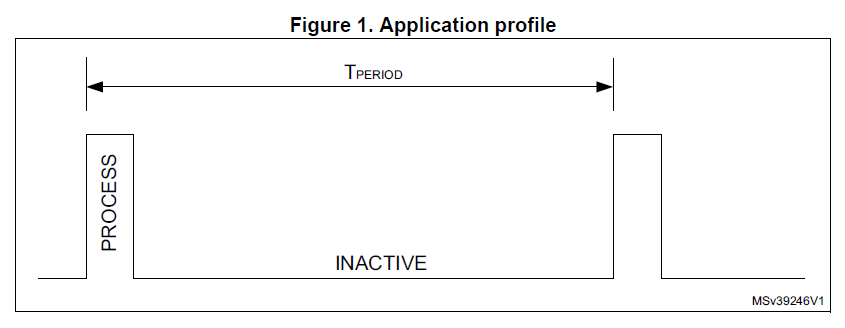
\includegraphics[scale= 0.6]{Application profile.png}
    \caption{Diagram showing a general low power operation profile  for the micro controller with two distinct phases: Process and Inactive occuring over a period T}
    \label{fig:appr}
\end{figure}

Figure \ref{fig:appr}

above details a typical low power operation Which can be expected from the buoy For a typical application, we consider two main phase:
\begin{enumerate}
    \item Process phase: System is in run mode with peripherals are active at regular intervals.
    \item Inactive phase: System is asleep until RTC/GPIO event.
\end{enumerate}

Once the buoy has finished an active routine, the system becomes inactive between samples. The buoy is designed to operate in routines occurring once every half an hour. Once the routine is complete, it still has to wait an extremely long time before it is required again. This is the inactive between sample mode and consider this our period of inactivity where we can place the device in the lowest possible state with very little concern for wake-up time or peripheral settings. \par 
Therefore, the following power modes were selected for each phase of the system's operation

\begin{table}[H]
    \centering
    \caption{Table showing the power mode selection for each phase of the Buoy's operational cycle}
    \begin{tabular}{|c|c|c|}
    \hline 
        Phase &  Power Mode & Current Draw \\
        \hline
        Process & Run Mode & 1.16mA\\
        Inactive & Standby Mode & 710nA\\
        \hline
    \end{tabular}

    \label{tab:powmode_cycle}
\end{table}

Table \ref{tab:powmode_cycle} above shows the estimated current consumption taken from the STM32L4 datasheet. The Current Value for Run Mode was bench-marked using a Dhrystone Test with an system clock of 24MHz and code loaded from Flash. The Inactive current draw was estimated with a Low Speed External Oscillator supplying the Real Time Clock. 

\subsection{Clock Selection}

The biggest Consideration with system operation is clock speed and source. The STM32l4 has 5 possible options: 3 internal oscillators (MSI,LSI,HSI) and 2 external crystal oscillators (HSE and LSE). Since the buoy will be inactive for long periods of time, an accurate 1Hz reference signal is required to keep calendar date and time. In addition, The STM32 microcontroller features a variety of wake up options to transition from low power mode to run mode
\begin{enumerate}
    \item Internal  configurable Alarm
    \item Periodic Wake Up Alarm
    \item External Wake Up Pin
\end{enumerate}

These options are made available through an internal Real Time Clock on the STM32L4 microcontroller. The peripheral can receive input from multiple clock sources such as an external Low Speed Oscillator (LSE), an internal Low Speed Oscillator (LSI) or an internal High-speed Oscillator (HSI). The peripheral also allows for fast and simple data storage during extreme power down modes. When the device enters shutdown mode, RAM is turned off, therefore all data will be lost. The RTC has 32 back up registers capable of retaining 1Kb of data when the device is powered down. \par 

these clock sources will provide power to the peripherals as well as  According the reference manual, the real time clock must be clocked from the LSE 32.768KHz crystal in order to provide an accurate calendar function therefore, the RTC must be clocked from the LSE no exceptions. The external crystal oscillators provide high precision clock speed with extremely low drift however, the power consumption of these oscillators are much higher than the internal RC. The clock configuration of the STM32L4 allows for a combination of these oscillators in a phase locked loop (PLL) which allows for a greater degree of accuracy at desired speeds. The final clock configuration parameters are shown in the table below:

\begin{table}[H]
    \centering
    \caption{configuration parameters for the system clock and Real Time Clock including sources and frequencies}
    \begin{tabular}{|l|l|}
    \hline
    Run Mode System Clock Source: & MSI and LSE in a PLL Configuration \\
    \hline
     Clock Frequency: & 24 MHz \\
     \hline
     Shut Down Mode Clock Source: & LSE \\
     \hline 
     RTC Clock Frequency & 1 Hz \\
     \hline 
     LSE Clock Frequency  & 32.768 KHz \\
     \hline 
    \end{tabular}
    \label{tab:clock_conf}
\end{table}

\section{Firmware Overview}

In a multi-sensing system, it is important to manage the interactions and data flow between the various aspects of the system to ensure the device operates in a predictable, manage manor. To achieve this, a state machine can be implemented to provide a high-level form of control over the system. This can be achieved by decomposing the overall function of the buoy into a series of finite states. These states are connected through a series of transitions which can be described using Boolean techniques. Through this, the buoy retains a modular structure both in firmware and in hardware which can allow for additionally sensors and functions to be implemented seamlessly.\par 


\subsection{Execution}

The goal of the buoy is to sample environmental, GPS and power data at a fixed rate. This rate $T_{sample}$ will be used to describe the period between sampling the devices. Each Sample will be condensed into a byte packet and stored in flash memory at a sector. After every 4 samples, the device will load the packets from memory into a buffer and transmit the data. When the device exits this state, it will reset the sample count and repeat until the buoy is turned off or loses power. The buoy can therefore be broken down into a set of finite states which are shown below:

\begin{enumerate}
    \item \textbf{Initialisation State:} The device initializes the counter and verifies the sensors.
    \item \textbf{Reset State:} Counter and memory Variables are Reset
    \item \textbf{Sample State:} During this state, the device actively receives data from the sensors and stores them into a packet which is then saved to Memory
    \item \textbf{Sleep State:} The device enters this state between samples and active states. Here, the device will remain in this state for a time $T_{sample}$. After which, the buoy will wake up 
    \item \textbf{Transmit State:} The device will load the data from memory and transfer to the Iridium Modem Buffer. Upon successful transmission, it will enter the Reset state
\end{enumerate}

Each state will control which routines are performed during the function and provide the system with information on the current status of the device. Should the device encounter a hardware reset, the system can recover and predict the action it needs to take based on the last state the system was in. A typical system run is shown in the figure below:

\begin{figure}[H]
    \centering
    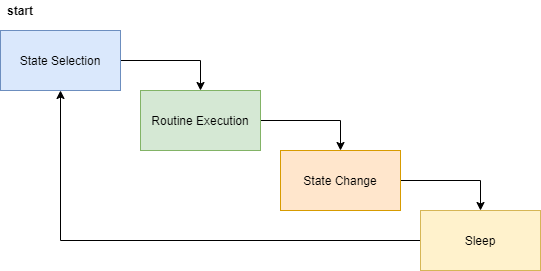
\includegraphics[scale = 0.5]{state Run.png}
    \caption{Diagram showing the steps executed from wake up when }
    \label{fig:state_run}
\end{figure}

The inputs to the state machine are:
\begin{enumerate}
    \item C: a 2-bit integer signifying the number of samples performed $(0 \leq N <4)$
    \item T: Variable that matters when the system is asleep. Signifies whether the system has been in sleep mode for a time defined by the constant value $T_{wake}$
\end{enumerate}

The system has no explicit outputs however, the state machine is used to control which routines will be executed during the execution phase of the program. Therefore, the outputs can be considered as the Routine Rx as shown below:
\begin{enumerate}
    \item $R_{sample}$: Sensor sample routine, this can involve all the sensors or just a select number. For simplicity's sake, this period implies all sensors will be sampled from
    \item $R_{sleep}$ : Device is in a sleep state and will wake up when the periodic wake up unit counts to a time $T_{wake}$
    \item $R_{Transmit}$ : Satellite Transmission Routine
\end{enumerate}

Given the following information, the Algorythmic State Machine (ASM) chart is derived and shown in the figure below

\begin{figure}[H]
    \centering
    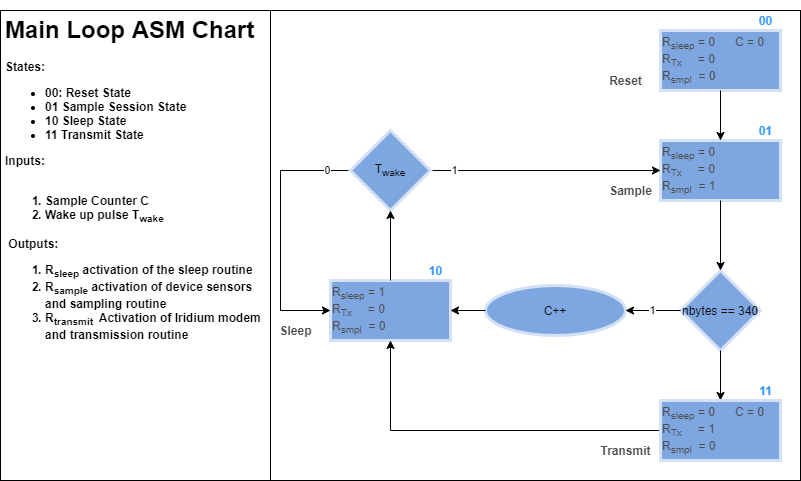
\includegraphics[scale=0.6]{Main Loop ASM Chart.png}
    \caption{ASM chart for the proposed program to run on the processor showing entry/exit conditions and functions to be run during states.}
    \label{fig:ASM_chart}
\end{figure}

Figure \ref{fig:ASM_chart} above shows an abstract representation of the logical flow of the program. A typical run from the system will have the buoy initialised and calibrated before entering the main loop where it will alternate between active sampling and inactive sleep mode until enough data has been collected to transmit. This allows the Iridium modem to only be turned on when needed thereby significantly conserving energy while allowing for the system to sample as much as possible. The variable $T_{wake}$ is user defined and sets the sample rate of the system For this application it has been set to 30 minutes. The device will sample 4 times with 30 minute intervals in-between and transmit the data on the 4th cycle i.e. every 2 hours.

The RTC periodic wake up unit is used as a counter in deep sleep mode. This is a 16-bit down-counting Auto Reload Register that generates an interrupt on an internal wake up line when the system has Slept for a length of time T as defined by the user. In addition, the sample counter gets reset after every transmission state and when the buoy enters a reset state. The number of samples before transmission is chosen to be 4 to optimize packet size for the transmission buffer. Since the Iridium Buffer is 340 Bytes long and the Transmission rate is per 50 bytes, the goal is to transmit as much data that would fit into the buffer as possible. Too frequent transmissions incur a high data cost but result in data integrity. Too few transmissions can result in lost sample points if a transmission is not received.

\subsection{Asynchronous Behaviours}
Asynchronous behavior describes all functionality that occurs outside of the main loop. This can come from Interrupts/ External events which causes the system to exit the main loop regardless of state and execute the code. This can occur from the following sources:

\begin{enumerate}
    \item Interrupts
    \begin{enumerate}
        \item Iridium Message Received (Ring Alert)
        \item IMU Event Detection (Collision / Free-fall detection)
    \end{enumerate}
    \item Events
    \begin{enumerate}
        \item Low power detection.
        \item Brown out detection.
        \item Software resets.
        \item Watch Dog resets.
    \end{enumerate}
\end{enumerate}

These events take precedence over the main loop function. The table below shows the entry/exit conditions. Functionality as well as return state after exit. A full description of events, interrupts, and the protocols for handling them are shown in tables \ref{tab:Int_desc_RI} to \ref{tab:Ev_desc_SWR} in Appendix \ref{sec:evt}. The figure below shows how the event handling procedure is sequenced in the main program:

\begin{figure}[H]
    \centering
    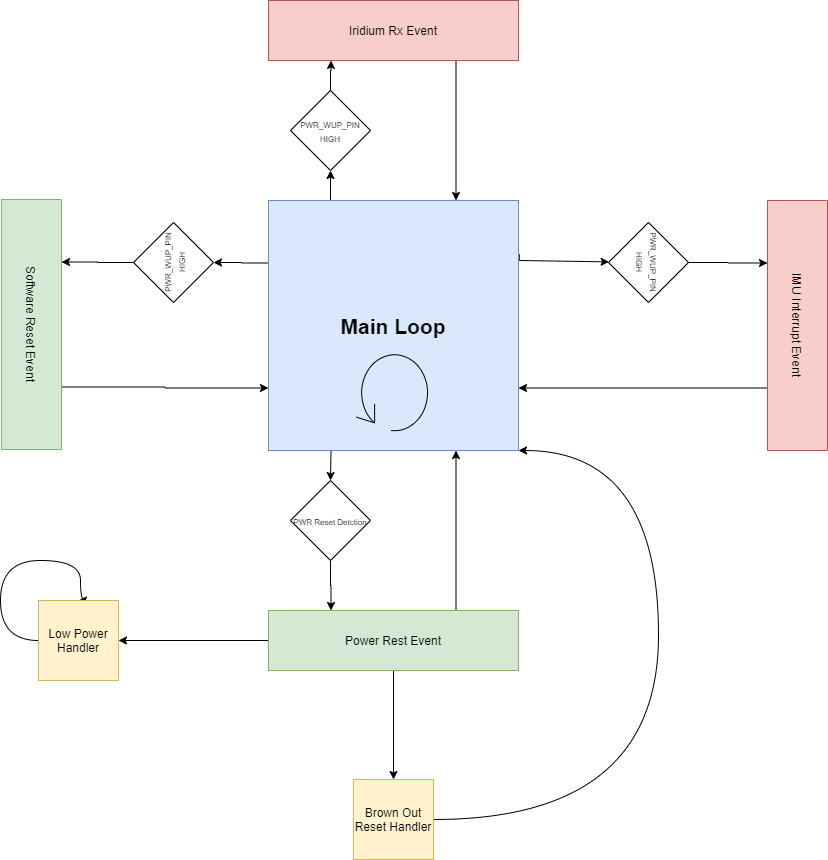
\includegraphics[scale=0.4]{Asynchronous State diagram.png}
    \caption{Application Diagram with Event and Interrupt sequencing}
    \label{fig:main software}
\end{figure}

States are represented by integers on the system and are stored in the back up registers of the RTC. These registers keep data even when the device is in low power mode or a software reset has occurred therefore making them the perfect storage location. The State Variable holds the value of the current state of the buoy. This variable is stored in two locations: When the system is in run mode, the value is stored in the global variable \textit{Current\_State}. When the device is in a deep sleep state, The variable is stored in the RTC Back up registers at byte 0 of Back-Up Register 0. Upon wake up, the value is loaded from the register and placed in the global variable.

The main loop follows a sequential state transition as described in Figure \ref{fig:main software}. To achieve this, at the start of each loop, the program reads the value stored in the state variable. This determines what the previous state was. Based on this value, the new state is determined and stored in the state variable. This process is shown in the figure below.

\begin{figure}[H]
    \centering
    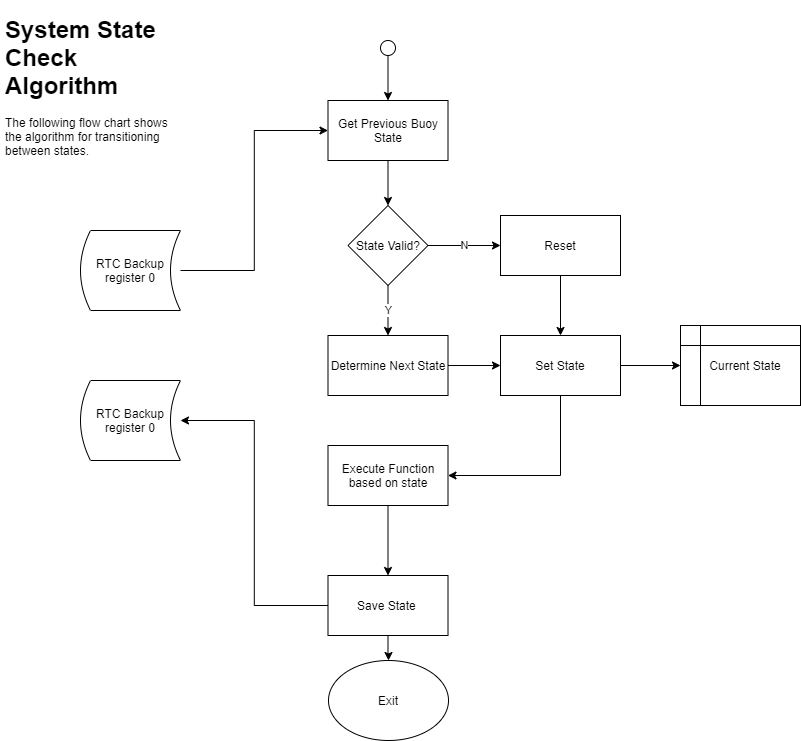
\includegraphics[scale=0.5]{State Check Algorithm.png}
    \caption{Flow chart for the state-check algorithm}
    \label{fig:state_check}
\end{figure}

Figure \ref{fig:state_check} above shows the algorithm for selecting and transitioning between states. This algorithm allows for states to be linked in any order and, most importantly, Separates the state selection from the state function. By separating these two concepts, a more modular framework is created. This allows for the addition of more states and transitions without modifying the routines that are currently in place. This allows for device functions to be turned on and off as desired without drastic changes to the firmware.

Finally, Asynchronous States take a higher precedence over the main loop states and therefore are checked before the state check shown above. The order of precedence is shown in the table below:
\begin{table}[H]
    \centering
    \caption{Table showing the types of states that the system checks for ordered by priority with 1 being the highest priority and 3 being the lowest}
    \begin{tabular}{|l|c|}
         \hline
         Name & Priority \\
          \hline
         Power Event & 1 \\
         \hline
         Asynchronous Interrupt & 2 \\
             \hline
         Sequential State & 3 \\
             \hline
    \end{tabular}

    \label{tab:state_prio}
\end{table}

Power Events generate a system reset and raise a flag in the PWR Status Register. When the flag is set, the program enters the handler and, if the event is non-fatal, returns to the main loop. The following flow chart shows an example of such a case for a Brown Out Event

\begin{figure}[H]
    \centering
    \includegraphics[scale = 0.4]{Brown Out Reset Handler Flow Chart.png}
    \caption{Diagram showing the algorithm for Brown Out Event Recovery and Handling}
    \label{fig:evt_handle}
\end{figure}

Some sensors have interrupt pins and can be configured to trigger upon detection of a specific event. When this happens, the sensor will send a digital high on the interrupt pin. On the processor side, a hardware interrupt is generated and the software handles the interrupt. An example of such a prceedure is shown in the figure below

\begin{figure}[H]
    \centering
    \includegraphics[scale = 0.5]{Asynchronous State flow chart.png}
    \caption{Diagram showing the algorithm for handling an external interrupt from a Wake Up pin connected to one of the modules}
    \label{fig:int_handle}
\end{figure}

By connecting these pins to external wake up pins, the buoy is capable of event detection in deep sleep mode. If an event is detected while in deep sleep, the interrupt causes the buoy to wake up and resume from the beginning. No interrupt handler is entered at this point. A flag is set the PWR\_SR at the position of the wake-up pin it detected. The buoy will enter the asynchronous state depending on which flag is set and will execute the routine associated with it.  When the buoy wakes up from an internal wake up timer, the pins are reconfigured into GPIO EXTI mode which allows the buoy to receive interrupts when active. Note: by keeping the buoys configured as wake up pins, the system will reset when an interrupt is detected.

\subsection{Subsystem Execution}

When a module is is being used at any point in the program. The micro-controller will execute an initialise routine. This will enable any required peripherals for communication with the subsystem. This function will be called before every sample period in case the system encounters a power surge or an unexpected reset. Additionally, placing the micro controller in deep sleep mode results in the registers being reset upon wake up. The initialisation routine is specific to each micro-controller and includes the following:

\begin{enumerate}
    \item High Level Communication Peripheral Configuration
    \item Low Level Pin configuration
    \item Sensor Verification function
    \item Sensor Configuration function
    \item Return Status
\end{enumerate}

The outcome of the initialisation routine is evaluated based on a return status from the function. Items 1 - 3 are included to configure the subsystem to adhere to the functional requirements in table \ref{tab:sys_specs}. Sensor Verification functions are included to satisfy acceptance Tests AT001 and provide evaluations for acceptance tests AT002 and AT004. The initialisation function is designed handle fail modes by evaluating the system's failure return type and responding in accordance with the protocols outlines in acceptance Test 2. Initialisation routines for each subsystem is provided in Appendix \ref{fig:Init_diagram_gps} to \ref{fig:Init_diagram_mpu}

If the initialisation was successful, the program will continue using the module in the firmware. Should a failure occur, the system will attempt to reconnect with the device a predefined number of times. In case of a critical failure, the system will acknowledge that it can no longer use the device and will continue the main firmware without it. The resulting behaviour is shown in the table below:

\begin{table}[H]
    \centering
     \caption{Table Showing the device behaviour in case of a critical failure in one or more of the subsystems. Critical failures are defined in AT006 (table \ref{tab:AT006}) testing protocol.}
    \begin{tabular}{|l|l|l|}
    \hline
       \textbf{Device Failure Case:}  & \textbf{Impact:} & \textbf{Result:}\\
       \hline
       Iridium & Critical & No data will be transmitted from the buoy \\
       \hline
       Flash Chips & Critical & Data will be lost when power is reset \\
       \hline
       GPS & High & GPS data will not be captured \\
       \hline
       MPU6050 & High & Unable to measure Waves in Ice  \\
       \hline
       Environment Sensor & Medium & Environmental data will not be captured \\
       \hline
       Power Monitor & Low & Current and voltage measurements will not be captured \\
       \hline
    \end{tabular}
    \label{tab:exe_subsy_Failiure}
\end{table}
\section{Data Management}

A critical consideration for the system is the flow of data and memory Management. The flash chips provide a solution for permanent storage however, it is critical that data integrity be maintained.Some form of data organization must be implemented for intelligent retrieval/ storage of data in a meaningful way. In addition, the system requires some form of back up should the device be unable to connect to the flash chips. \par 

The flash Chips being used are AT45DB641E SPI Serial Flash Chips. Each chip can hold up to 64Mbit of data. Data can be read/ written at speeds of up to 85MHz of 15MHz in low power mode. The device is low power with high data retention requiring a supply voltage of 1.7V – 3.6V and draws a maximum of 11mA in Active Read mode thereby making it one of the lowest power consumption components in the system. In addition, the device comes with 2 x 256byte buffers that can store data while a read/ write operation is taking place. Memory is Organized into sectors (2 – 256 Kbs long), blocks (2kB long) and pages (256 bytes) with write, read and erase options at each level. \par 

In this section, the data requirements from each sensor is listed. The optimal storage strategy is to convert the measurements into binary data and store as an array of bytes at known locations in an array. The data requirements for each component is listed below

\subsection{Drift Data Acquisition}
This section describes how data is aquired from the sensors to form an Ice Drift measurement. Readings are taken from the GPS and environmental sensor with the power monitor being sampled to provide an update on the buoys performance.\par 

The GPS is sampled 4 times over a given interval. The interval between samples can range from 15 minutes to 30 minutes. At each sample point, the following data is recorded

\begin{enumerate}
    \item Time and Date Information
    \item Geographical Coordinates
    \item Dilation of Precision
    \item Diagnostic Information
\end{enumerate}

%Time and Date information 
By Default, the Ublox Neo GPS series uses the National Marine Electronic Standards (NMEA) \footnote{Information about NMEA messaging on the UBlox Neo GPS is taken from the Interface description here: \url{https://www.u-blox.com/sites/default/files/NEO-M9N_Interfacedescription_\%28UBX-19035940\%29.pdf}} format to send messages. This message structure can vary depending on the type of message being sent/ received however, these message follow the same format:

\begin{table}[H]
    \centering
    \caption{ Breakdown of a typical NMEA message string with fields indicating start/stop sequences and character information.}
    \begin{tabular}{|c|c|c|c|c|c|}
    \hline
     \$    & \multicolumn{2}{|c|}{Address} & Data Field & checksum & End Sequence\\
     \hline
     \multicolumn{1}{c|}{} & TT & SSS &\multicolumn{3}{c}{} \\
      \cline{2-3}
    \end{tabular}

    \label{tab:GPS_data_format}
\end{table}
\begin{itemize}
    \item \$ - Character denoting the start of the sequence
    \item Address - This is a 5 character sequence that is used to provide information on the Talker ID (TT) and the the type of information in the Payload (SSS)
    \item Data Field - Data in this field is formatted as a character sequence separated by commas. This field holds the payload specified by the payload information characters in the address field
    \item checksum - Sequence of characters denoted by a "*" and followed by two bytes in ASCII hexadecimal format. These values are calculated by performing an XOR operation on all the bytes between the "\$" and "*" characters
    \item End Sequence - 0x0D, 0x0A denotes the end of the  NMEA message
\end{itemize}

Each NMEA message holds different information and can vary in the message size. To ensure a standardised data flow, The following table shows the NMEA messages that were selected and the data as well as the format of each of the fields:

\begin{table}[H]
    \centering
    \caption{Description of ZDA Message string showing variables, description and how the example datum 5th September 2002 08:27:10 am is stored}
    \begin{tabular}{|l|l|l|}
    \hline
     \multicolumn{3}{|c|}{\textbf{ZDA - Time and Date}}\\
     \hline
    \textbf{Description:} & \multicolumn{2}{l|}{Datum information in UTC representaion}\\
     \hline
     \textbf{Variable Name} & \textbf{Format}& \textbf{Example} \\
     \hline
      UTC Time & hhmmss.ss & 082710.00 - 08:27:10 am\\
      \hline
      UTC Day  & dd & 05 - 5th \\
      \hline
      UTC Month & mm & 09 - September\\
      \hline
      UTC Year & yyyy & 2002 \\
      \hline
      Time Zone Hours & hh & 00 (+00)\\
      \hline
      Time Zone Minutes & mm & 00 (+00)\\
      \hline
    \end{tabular}
    \label{tab:NMEA_ZDA}
\end{table}

\begin{table}[H]
    \centering
    \caption{Description of GSA Message string showing variables, description of parameters and how the variables are stored}
    \begin{tabular}{|l|l|l|}
    \hline
     \multicolumn{3}{|c|}{\textbf{GSA - Fix Diagnostic}}\\
     \hline
    \textbf{Description:} & \multicolumn{2}{l|}{ DOP, number of satelites and fix type}\\
     \hline
     \textbf{Variable Name} & \textbf{Format}& \textbf{Example} \\
     \hline
     Opperation Mode & A/M & A - Automatic\\
      \hline
     Navigation Mode  & Number (1-3) & 1 - No Fix \\
      \hline
      Satelite ID & Number  & 29 - Satelite number \\
      \hline
      Direction & C & E - East \\
      \hline
      PDOP & Float & 1.91 \\
      \hline
      HDOP & Float & 1.18 \\
      \hline
      VDOP & Float & 1.14 \\
      \hline
    \end{tabular}

    \label{tab:NMEA_GSA}
\end{table}

\begin{table}[H]
    \centering
    \caption{Description of GLL Message string showing variables, description and how a set of coordinates e.g. (47$\degree$17.11364'N,  8$\degree$ 33.91565' ) is stored}
    \begin{tabular}{|l|l|l|}
    \hline
     \multicolumn{3}{|c|}{\textbf{GLL - Geographic Coordinates and Fix}}\\
     \hline
    \textbf{Description:} & \multicolumn{2}{l|}{ latitude and longitude with postional fix information}\\
     \hline
     \textbf{Variable Name} & \textbf{Format}& \textbf{Example} \\
     \hline
     Latitude & ddmm.mmmmm & 4717.11364 - 47$\degree$17.11364'\\
      \hline
     Direction  & C & N - North \\
      \hline
      Longitude &dddmm.mmmmm & 00833.91565 - 8$\degree$ 33.91565' \\
      \hline
      Direction & C & E - East \\
      \hline
      Fix Status & A & A - Valid\\
      \hline
    \end{tabular}

    \label{tab:NMEA_GLL}
\end{table}

The UBlox Neo Module continuously outputs data at a fixed rate of 1Hz \cite{UBLOX_M9N_INTERFACE} through Universal Synchronous/Asynchronous Transmission. The device comes preset with certain messages activated. The required messages need to be enabled by writing to the \textit{CFG-MSGOUT} register. Then, Message parsers were written to extract the information for the aforementioned message strings and convert them into binary representation. These message parsers contain a check for validity. This algorithm first checks that the data follows the correct NMEA formatting as shown in Table \ref{tab:GPS_data_format}. Then it analyses the Address to ensure that the Talker ID and and Message ID are valid. Finally it calculates the two byte checksum by performing an exclusive or on all the bytes in the data field and compares them to the checksum bytes that were sent with the packets. Message parsers were written for GLL, GSA and ZDA messages and were called based on the return status of the validty check.
The following table shows the memory allocation for each variable. 
 \begin{table}[H]
     \centering
     \caption{Data collected from the GPS in a single sample session.}
     \begin{tabular}{|l|l|c|}
     \hline
    \textbf{Variable Name}  &  \textbf{Variable Type} & \textbf{Size (bytes)}  \\
    \hline
          Epoch Time & Unsigned 32-bit Int & 4  \\
          Latitude & signed 32-bit Float & 4 \\
          longitude & signed 32-bit Float & 4 \\
          HDOP & Unsigned 8-bit Int[2] & 2\\
          VDOP & Unsigned 8-bit Int[2] & 2\\
          PDOP & Unsigned 8-bit Int[2] & 2\\
          Diagnostic Info & Unsigned 8-bit Int & 1 \\
          \hline
          \cline{3-3}
          \multicolumn{2}{r}{Total: } & \multicolumn{1}{c}{19}\\
          \cline{3-3}
          \cline{3-3}
          
     \end{tabular}
     \label{tab:GPS_Data}
 \end{table}
 
 Time and date information were combined and converted into Unix Epoch Time. This represents the number of seconds that have elapsed since a defined epoch (1 January 1970) which allows for a single, 4-byte variable to represent both time and date. Geographic coordinates have been converted into singed 32-bit floats with the sign representing the direction of the coordinate. The coordinates were then split into an array of 4 unsigned 8-bit integers and recombined using IEEE-754 as a standard. The dilation of precision represents a value between 0 and 99.99 therefore, the optimal storage solution is to allocate a byte for the digit and a byte for the precision. Finally, diagnostic information includes the Fix type and the number of satellites. A maximum of 15 satellites can be used to determine a position This data can be stored in the lower 4 bits of a single 8-bit integer. The fix type is a number from 1-3 therefore only taking up 2 bits.\par 
 
 
The BMP contains 2 onboard Analog To Digital Converters (ADCs) which are used to convert the pressure and temperature measurements into unsigned byte strings.Each measurement is stored as 3 unsigned 8-bit integers in 3 registers and must be read sequentially in order to get the full measurement. Once retrieved, the data must be combined into a 24-bit word which results in the raw, uncompensated ADC value. The BMP also contains a configurable Infinite Impulse Response (IIR) filter as well as configurable oversampling parameters for the pressure and temperature measurement. Data is read through an SPI communication interface into the micro-controller by performing a bust read of 6 bytes. To compensate for the mechanical effects of each sensing element, the device comes preloaded with a set of compensation parameters for the temperature and pressure reading \cite{BMP280_Datasheet}. The compensation algoriintthms are shown in Appendix \ref{fig:bmp_code_comp_P} and \ref{fig:bmp_code_comp_T}. The output of the compensation algorythm are shown in the table below

\begin{table}[H]
    \centering
    \caption{Description of output values from BMP280 post processing.}
    \begin{tabular}{|l|l|l|l|c|}
    \hline
         \textbf{Name }& \textbf{Type} &\textbf{Format} & \textbf{Example} & \textbf{Total Bytes}   \\
         \hline
          Temperature & signed 32-bit Integer & CCcc$\degree$C & 2508 - 25.08$\degree$C & 4\\
          \hline
          Pressure & signed 32-bit integer & PPPppp KPa & 100653 - 100.653 Kpa & 4\\
          \hline
          \multicolumn{4}{r}{\textbf{total:}} & \multicolumn{1}{c}{8}\\
          \cline{5-5}
          \cline{5-5}
    \end{tabular}

    \label{tab:BMP_output}
\end{table}

The INA219 samples Current across a shunt resistor of a known value. In thiss application, the shun resistor provided is $0.1\Omega$. The device also samples the Voltage accross the shunt resistor which passes through a programmable gain amplifier before being sampled by and ADC. The sensor stores data as 16 bit integers. Negative values are stored in two's compliment formed. Data is transferred via I2C to the microcontroller after the conversions have taken place. The sensor measure both shunt and bus voltage which, when combined, provide an estimate of the Load Voltage. The resolution of the values can be programmed as either 9-bit, 10 bit or 12 bit. When the device is initialised, it needs to be calibrated. Calibrating the device begins by specifying the User's power requirements and maximum current range. THe Bus range voltage is chosen as either 16V or 32V. The output of the calibration procedure is a 16-bit word that is written to the Calibration register. The algorithm used to calibrate the sensor for the SHARC Buoy application is outlined in Appendix \ref{fig:INA_Calib} with the following parameters:
\begin{table}[H]
    \centering
    \caption{ Description of parameters used to calibrate the INA219 current sensor}
    \begin{tabular}{|l | l|}
    \hline
         \textbf{Maximum Bus Voltage}& 16V \\
         \hline
         \textbf{Maximum Expected Current} & 1.2A \\
         \hline
         \textbf{Shunt Resistor} & 0.1 $\Omega$ \\
         \hline
         \textbf{Shunt Voltage Range} & $\pm$ 160mV\\
         \hline
    \end{tabular}

    \label{tab:INA_Calib}
\end{table}

The Sensor calculates the power consumption as a signed 16 bit number by multiplying the Bus Voltage with the Current and placing it in the Power Register. The microcontroller performs a burst read of the Bus Voltage, Shunt Voltage, Current Voltage and power register and stores the values as signed 16 bit integers. The bus voltage register reserves the first 3 bits of the register for signal flags. Therefore, the bus voltage reading is shifted by 3 bits to the right to remove them. Finally, the Power reading is multiplied by the LSB size calculated in the calibration function which results in a signed 16 bit integer representation of the power in milliwatts. The data requirements are shown in the table below:

\begin{table}[H]
    \centering
    \caption{Description of output values from INA219 current sensor.}
    \begin{tabular}{|l|l|l|l|c|}
        \hline
        \textbf{Name }& \textbf{Type} &\textbf{Format} & \textbf{Example} & \textbf{Total Bytes} \\
        \hline
        Shunt Voltage & Signed 16-bit Integer & vvvmm & 18049 - 180.49mV & 2 \\
        \hline
        Bus Voltage & Signed 16-bit Integer & VVvvv & 08025 - 8.025V & 2 \\
        \hline
        Current & Signed 16-bit Integer & IIIii & 51234 - 519.23 mA & 2 \\
        \hline
        Power & Signed 16-bit Integer & PPPPpp &  28130 - 2813.00mW & 2 \\
        \hline
        \multicolumn{4}{r}{\textbf{total:}} & \multicolumn{1}{c}{8}\\
        \cline{5-5}
        \cline{5-5}
    \end{tabular}

    \label{tab:INA_Output}
\end{table}

\subsection{Wave Measurement Data}

This section describes how data is acquired for Waves in ice measurements. The Inertial Measurement Unit (IMU) provides 3 axes of acceleration and 3 axes of angular velocity which are the components used to estimate the significant wave height, dominant wave frequency as well as the spectra and co-spectra over the sample period. Wave Data sampling occurs after the 4th drift measurement is taken and the IMU is sampled. The sample frequency was chosen to be 5Hz to be above the Nyquist frequency of the dominant wave frequency.\par 

The MPU6050 IMU is a micro electrical-mechanical (MEM) based system. The device measures the inertial axis reading which is then digitised using a 16-bit ADC for each axis of the accelerometer and gyroscope. Communication is performed using I2C where the pin AD0 is used to set the I2C address. In addition, the device is fully configurable allowing for programmable ADC full scale resolutions and sample rates. The device also contains an on-board digital low pass filter, the bandwidth of which can be programmed through the \textit{CONFIG} register.\par 
The MPU6050 is an 8-bit device. Measurements from the ADC are split into 8-bit bytes and stored across 2 registers (one for the most significant byte, and one for the least significant byte). A burst read operation is performed to retrieve the data in the register. The two bytes are combined and stored as a signed 16-bit integer. This value is then multiplied by a sensitivity factor which results in a float representing either the acceleration in $ms^{-2}$ or the angular velocity in $\degree s^{-1}$. The sensitivity factor is determined based on the selected Full Scale Range of the accelerometer and gyroscope. Therefore, the following table gives a breakdown of a single sample of IMU data:

\begin{table}[H]
    \centering
    \caption{Description of output values from the MPU6050 IMU showing variable name, size and significance}
    \begin{tabular}{|l|l|c|}
    \hline
    \textbf{Name} & \textbf{Type} &\textbf{Total Bytes} \\
    \hline
     x-axis Acceleration & Signed 16-bit Integer & 2\\
     \hline
      y-axis Acceleration & Signed 16-bit Integer & 2\\
     \hline
      z-axis Acceleration & Signed 16-bit Integer & 2\\
     \hline
     x-axis Angular Velocity & Signed 16-bit Integer & 2\\
     \hline
     y-axis Angular Velocity & Signed 16-bit Integer & 2\\
     \hline
     z-axis Angular Velocity & Signed 16-bit Integer & 2\\
     \hline
     \multicolumn{2}{r}{\textbf{total:}} &\multicolumn{1}{c}{12}\\
     \cline{3-3}
     \cline{3-3}
    \end{tabular}

    \label{tab:IMU_data_outl}
\end{table}

From our user requirements the sample period for collecting wave data is a minimum of 15 mins. Average ocean wave sample periods are recorded at 20 mins sometimes even as high as 30 mins for significant wave height. Using Nyquist sample theory, the dominant wave frequency occurs at about 1 Hz. Sampling at 2 Hz \cite{kohout2015device} is a bare minimum however, 5Hz is recommended. 

\begin{table}[H]
    \centering
    \begin{tabular}{|l|l|}
    \hline
      \textbf{Sample Period: }   &  20 minutes\\
      \hline
      \textbf{Sample Frequency:} & 5Hz \\
      \hline
      \textbf{Accelerometer Full Scale Range:} & $\pm 2g$\\ 
      \hline
      \textbf{Gyroscope Full Scale Range:} & $\pm 500\degree s^{-1}$\\
      \hline
      \textbf{Digital Low Pass Filter Bandwidth:} & $92Hz$\\ 
      \hline
    \end{tabular}
    \caption{Paramaters of the IMU and their configured value for this application}
    \label{tab:IMU_param}
\end{table}

Finally, the total data accumulated over the required sample period is shown in the table below

\begin{table}[H]
    \centering
    \caption{Breakdown of data accumulated from the IMU with the sample parameters mentioned in table \ref{tab:IMU_param}}
    \begin{tabular}{|l|l|}
    \hline
    Sample Frequency     &  5Hz\\
    \hline
    Sample Period        & 1200s\\
    \hline
    Number of Samples    & 6000 \\ 
    \hline
    Bytes Per Sample     & 12 \\
    \hline
    \multicolumn{1}{r}{\textbf{total:}} & \multicolumn{1}{l}{72000 bytes}\\
    \end{tabular}

    \label{tab:IMU_data_total}
\end{table}

Therefore, a total of 72kB is collected from each session. With the current memory configuration. a single sample can occupy 0.9\% of a single Flash chip. However, due to the low bandwidth of the Iridium modem, IMU data would need to be split into packets of 340 bytes. This would require 212 transmissions to deliver a single set of data. This is not advisable due to the high current consumption of the modem as well as the long transmission times. To send all data, advanced compression techniques or a robust wave data processing algorithm needs to be implemented which falls outside the scope of this project.For testing purposes, as a proof of concept, the IMU sample period was reduced to 5.6s which resulted in 28 samples or 336 bytes of data.  

\section{Data Flow}
\begin{table}[H]
    \caption{Total drift data collected during a single sample point}
    \centering
    \begin{tabular}{|l|c|}
      \hline
      \textbf{Device Name}   &  \textbf{Total Data (bytes)}\\
      \hline
       GPS  & 19 \\
       Environmental Sensor & 8 \\
       Power Monitor & 8\\
       \hline
       \multicolumn{1}{r}{Total} & \multicolumn{1}{c}{35}\\
       \cline{2-2}
       \cline{2-2}
    \end{tabular}

    \label{tab:total_data}
\end{table}

Drift data is collected every half an hour with a transmission occurring after 4 samples. The total data collected before sampling is 140 bytes. The Iridium modem has a maximum transmission buffer of 340 bytes. Therefore, all data can be transmitted at once without any advanced transmission routines required. A custom struct was defined to hold all data in a central location.

\begin{figure}[H]
    \centering
\begin{lstlisting}
/*
 * @brief: Structure to store data from GPS in an organised format. Note: custom data types from HAL_GPS.h
 */
typedef struct
{
	uint32_t Etime;			//UTC Epoch representation of time
	Coord_t  coordinates;	//GPS coordinates
	Diagnostic_t diag;		//Diagnostic information
	uint32_t env_Temp;		//Environmental temperature
	int32_t  atm_Press;		//Atmospheric pressure
	int16_t  shunt_v;       //Shunt voltage (mv)
	int16_t  bus_v;			//Bus voltage   (mV)
	int16_t  current;       //Load current (mA)
	int16_t  power;			//Power consumption (mW)
}GPS_Data_t;
\end{lstlisting}
    \caption{Data struct for storing drift data collected from the sensors during a sample period where Coord\_t and Diagostic\_t are shown in Appendix \ref{fig:data_coord_t} - \ref{fig:data_Diagnostic_t}} 
    \label{fig:data_drift_struct}
\end{figure}

The struct is populated with data as each sensor completes its sampling. If a sensor fails or is unable to return valid data, the field is left blank and the program continues to sample from other sensors. This ensures that the program is robust when handling sensor fail error to meet the criteria for acceptance test AT004 in table \ref{tab:AT004}. Once the sensors have finished sampling, the data is condensed into a packet structure and stored in memory. The diagram below shows the structure of a single packet

\begin{figure}[H]
    \centering
    \includegraphics[scale=0.4]{Drift Packet Diagram.png}
    \caption{Diagram showing the structure of a drift data packet including byte position, size and data being collected}
    \label{fig:packet_structure}
\end{figure}

Each Packet begins with a Header. This is an 8-bit value to give information about the data in the payload. This value consist of a 4-bit identifier (0x0 for drift data) as well as a 4-bit number indicating the sample number (1 - 4) before transmission. Data is stored sequentially in little endian format as shown in figure \ref{fig:packet_structure} above. A '\\r' character is used to indicate the end of the packet. This increases the total data requirement from 35 to 37 bytes per sample however, by adding the tail and the header, data integrity is maintained and allow for the standardisation of data transmission.\par  

IMU data however, is of uniform type therefore, no special structures needed to be created. Data from the IMU is stored in an 8-bit buffer array with the most significant byte of the measurement first. Much like the drift buffer, The data was combined into a packet with a header created at the beginning. The header was given the value 0x57 or \textit{"W"} to identify the packet as an IMU data packet. Then the data occupies the remaining bytes with the final byte of the packet assigned to the '<cr>' character to indicate the end of the packet. \par 

Data is stored in the flash chips in packet structure form in the first page of the first available flash chip. Packets are stored sequentially until the device enters transmit state. All data is downloaded from memory and uploaded to the Iridium transmission buffer. The device initiates 2 transmission sessions. First the drift data is uploaded and transmitted, Then the IMU data.Upon successful transmission, the data is sent via satellite network to the Rock7 Rockblock server. The data is saved to a user's account and sent to their email address where the data can be downloaded as an attachment. The diagram below shows the flow of data from the sensors to the user 

\begin{figure}[H]
    \centering
    \includegraphics[scale = 0.5]{Data Flow Diagram.png}
    \caption{Diagram showing the flow of data during a cycle of the buoy. The data is sampled by the sensors and converted into packet form where it is stored until it is ready to be transmitted. The transmitted data arrives at a server and is sent via email to the user}
    \label{fig:data_flow}
\end{figure}

\chapter{Platform design}
\label{sec:ch3_platform}

In this chapter, the hardware design for the buoy is given based on the user requirements and technical specifications given in Chapter \ref{ch:ch3}. This chapter begins with a description of the mechanical features and how the design accommodates the electronic sub systems while meeting the functional requirements outlined in Table \ref{tab:hard_funcreqsl}. Next, a description of the component selection is given for each of the critical subsystems identified in table \ref{tab:subsys}. Finally, the chapter will conclude with a description of the hardware synthesis and final design considerations for the buoy. \par 

The Initial system design was performed by Son and Vorajee in 2018 which strongly influenced the design choices discussed in the forthcoming sections. Furthermore, MacHutchon designed the original buoy with modifications by Verrinder to accommodate the buoy. Verrinder designed the physical enclosure and electronic hardware subsystems for the first (V1) and second (V2) versions of the buoy with further design contributions from Jacobson (V1,V2) Cloete (V1) and Pead (V2).
\section{Mechanical Features}

The mechanical design for the system falls outside the scope of this project however, it forms an integral part in protecting the electronics. The principle goal of the mechanically features are to anchor the device to the ice floe and protect it from the harsh environment. A buoy stand was designed by Keith Hutchinson with the University of Cape Town Workshop to satisfy this requirement. The stand is 1.2m tall with a base cross section of 0.71m and contains a cylindrical housing at the top where the device will be placed. A screw hole in the side of the stand allows the buoy to be fast-end to the stand to prevent it from falling out. The base of the stand is pyramid shaped with metal spikes to anchor the system to an ice floe. Due to the height of the stand, the system may be susceptible to tipping. This has been overcome by constructing the base to be heavier than the top thereby lowering the center of gravity. The stand was originally designed for the Trident buoys and this design has been modified by increasing the radius of the housing. 

\begin{figure}[H]
	\centering
	\includegraphics[scale = 0.7]{buoy_stand.PNG}
	\caption{3D Render of the buoy stand.}
	\label{fig:stand}
\end{figure}

The second part of the mechanical subsystem is the physical buoy enclosure. The greatest challenge for designing this system was selecting a material that was both lightweight and low-temperature resistant. A decision was made to use High-Density Polyethylene which has excellent low temperature thermal properties. The enclosure was designed to fit the housing on the buoy stand while providing ample room for the antennas of the various communication modules. the enclosure was split into 3 parts: A top enclosure, a bottom enclosure and a connector block. A schematic of the enclosure is shown in the figure below

\begin{figure}[H]
	\centering
	\includegraphics{enclo_schem.PNG}
	\caption{2-D Drawing of the Buoy Enclosure showing the separate components}
	\label{fig:enclo_schem}
\end{figure}

\begin{table}[H]
	\centering
	\caption{Primary Measurements of the buoy enclosure taken from the schematic in appendex \ref{fig:full_schem} \ref{fig:bot_schem} \ref{fig:top_schem} \ref{fig:conblock_schem}}
	\begin{tabular}{||l  l c||}
		\hline
		\textbf{Component} &   \textbf{Dimension} &   \textbf{Value (mm)} \\
		\hline
		\hline
		\multirow{4}{*}{Top Enclosure} & height & 240\\
		&  diameter & 98  \\
		&  wall thickness & 4 \\ 
		& base thickness & 5 \\
		\hline
		\multirow{3}{*}{Bottom Enclosure} & height & 100\\
		&  diameter & 98  \\
		& thickness & 10 \\ 
		\hline
		\multirow{5}{*}{Bottom Enclosure} & height & 80\\
		&  outer diameter & 98  \\
		&  top inner diameter & 89.94  \\ 
		&  bottom inner diameter & 77.85\\
		&  O-ring Thickness & 2.6 \\
		\hline
	\end{tabular}
	
	\label{tab:enc_meas}
\end{table}

This design allows for easy access to the electronics as well as separation between the various subsystems. The connector block acts as a connection point for the electronics in version 1. This point of contact was a 3d printed connector for a vertically mounted PCB. In version 2, this was replaced by a row of screw holes around the connector block to connect a horizontal Stack of customised PCBs. This was found to greatly improve the robustness of the system and prevented components from breaking. The communication modules, microcontroller and sensors were mounted in the top enclosure while the batteries and power system were placed in the bottom enclosure. The power system was connected to the top enclosure through a drill hole in the connector block. The system was waterproofed by placing 2 o-rings on either side of the connector block. The top and bottom enclosure are fastened to the connector block using a a flat head counter sunk hex screw. Finally a drill hole in the connector block allowed the system to be secured to the buoy stand preventing it from falling out during deployment.

\section{Electronics}

The electronics for the system refer to the Communication subsystems, power electronics, sensors and processors. Due to project time constraints, the approach to developing the platform was to select off the shelf components that satisfied the requirements shown in table \ref{tab:sys_specs}. Further consideration was given to components that were low power (SP011, SP012) and cost effective components (SP013). Additionally, devices with intelligent operations were selected as this would allow us to effectively control the current consumption and operations of the device. These consisted of components with programmable settings such as digital sensors, actuators and modems. The following section gives an overview of the selection consideration for each subsystem

\subsection{GPS}

A Ublox Neo-7m was initially selected as it was easy to procure and has a small form factor. The module comes on a Waveshare breakout board which significantly decreases the development time. The board comes with an active patch antenna which has a gain of about 30dB. In addition, the component is low power with a relatively fast acquisition time and accuracy. The device also can be configured to output diagnostic information and Dilation of procession with the associated measurement which can provide a greater understanding of satelite connectivity in the region. However, by the time we requested more modules, the device was out of stock and had depreciated. To overcome this, we opted for the Neo-M9N module which had significantly improved performance at a higher cost. The table below shows a comparison of the two modules and their key performance parameters.

\begin{table}[H]
	\centering
	\caption{Comparison of key parameters between the initial Ublox Neo-7m gnss module and the updated Ublox Neo-N9M module}
	\begin{tabular}{|l |l |l|}
		\hline
		\textbf{Description} & Neo-7M & Neo-M9N\\
		\hline
		Positional Accuracy: & 2.5m  & 2.0m\\
		Communication Type: & UART, I2C, SPI & UART, I2C, SPI\\
		Cold-Start Time:& 30s & 26s\\
		Supply Voltage & 1.65V - 3.6V & 2.7V -3.6V\\
		Active Current Draw & 32mA &  42mA\\
		Price & R269 \footnotemark & R1,195.45 \footnotemark\\
		\hline
	\end{tabular}
	\label{tab:neo7}
\end{table}
\footnotetext[1]{from Digikey \url{https://www.digikey.co.za/} ordered on 09/2020} 
\footnotetext{from Microrobotics \url{https://www.robotics.org.za/} ordered on 19/12/2018}
The Neo 9-m offers improved performance at a higher cost and higher power consumption. This module comes on a Sparkfun breakout board with an option for an external u.fl antenna or an integrated chip antenna. The chip antenna however has a very small gain making it unsuitable to be used for this application. Therefore, an additional antenna was bought.

\subsection{Iridium}

The Iridium modem is critical for ensuring data can be transmitted from remote locations. When selecting a modem, key considerations were given to the physical size, Bandwidth as well as coverage. In addition, we require a module that is low powered and cost effective. For this reason, we have selected the Rock block 9603 modem which has the following key specifications. This is a module that contains an Iridium 9603 modem on a specially -designed power board. The device communicates via UART with the option for flow control. The module contains a 10-pin picoblade. The module contains 4 communications pins, 1 digital input pin and 2 digital output pins for interfacing with. Power is supplied either through a 5V pin or 3.3V pin in addition to the ground pin. A brief description of the pin out is given in the table below: 

\begin{table}[H]
	\centering
	\caption{Pinout for the Rockblock 9603 Iridium Modem}
	\begin{tabular}{c l l}
		\hline
		Pin Number: & Label & Pin Description\\
		\hline
		\hline
		1 & RXD & UART Output Pin \\
		
		2 & CTS & Flow Control Clear To Send\\
		3 & RTS & Flow Control Request To Send\\
		4 & NetAv & Network Available \\
		5 & RI & Ring Inidcator \\
		6 & TXD & UART Input Pin \\
		7 & OnOff & Sleep Control\\
		8 & 5V & 5V max supply pin \\
		9 & Li-Ion & 3.7V max supply pin \\
		10 & GND & Ground \\
		\hline
		\hline
	\end{tabular}
	
	\label{tab:ir_pinout}
\end{table}

The device communicates via UART through the RXD and TXD pins. The CTS and RTS pins are optional if flow control is required. The OnOff pin can be used to put the device to sleep which significantly improves power performances. Finally, The NetAv and Ring Indicator are notification pins that can be used to indicate whether there is sufficient signal to transmit as well as to notify when a message is waiting to be downloaded respectively. 

Finally, the key characteristics for the device are shown in the table below:

\begin{table}[H]
	\centering
	\caption{Table showing key parameters and performance characteristics taken from the datasheet}
	\begin{tabular}{|c|c|}
		\multicolumn{2}{l}{Mechanical Features:}\\
		\hline
		\textbf{Antenna: } & Patch or External SMA\\
		\hline
		\textbf{Temperature Rating:} & -40ºC to +85ºC\\
		\hline
		\textbf{Dimensions}  & $45.0 \times 45.0 \times 15.0$ mm  \\
		\hline
		\textbf{Cost: } & R2,850.56\\
		\hline
		\multicolumn{2}{l}{Power Characteristics:}\\
		\hline
		\textbf{Supply Voltage} & 5v or 3.7v Li-Ion \\
		\hline
		\textbf{Start-Up Current} & 450mA \\
		\hline
		\textbf{Active Current} & 100mA \\
		\hline
		\textbf{Sleep Current} & 200uA\\
		\hline
		\multicolumn{2}{l}{Communication:}\\
		\hline
		\textbf{Baudrate} & 19200 b/s \\
		\hline
		\textbf{ Data bits} &  8\\
		\hline
		\textbf{Stop bits} & 1 \\
		\hline
		\textbf{Parity} & none \\
		\hline
		\textbf{Max Upload size} & 340 bytes \\
		\hline
		\textbf{Max Download Size} & 270 bytes \\
		\hline
	\end{tabular}
	
	\label{tab:ir_specs}
\end{table}

\subsection{Sensors}

2 versions of the buoy were developed from 2019 - 2020 with different sensing capabilities. The first version consisted of a DS18B20 Temperature sensor. This was a low cost, small form factor device that interfaced over One-wire. In version two, this was dropped in favour of the Bosh Sensortech BMP280 sensor. The BMP featured improved sensing capabilities, temperature compensation as well as a programmable interface. In addition, the sensor contains both an ambient temperature sensor as well as a pressure sensor. A comparison of each device is given in the table below

\begin{table}[H]
	\centering
	\caption{Comparison of performance between the BMP280 and DS18B20 environmental sensors.}
	\begin{tabular}{|c|c|c|}
		\hline
		& \textbf{BMP280} & \textbf{DS18B20} \\
		\hline
		Temperature Range & $-40^\circ C \text{ to } 85^\circ C$&$-55^\circ C \text{ to } 125^\circ C$ \\
		\hline
		Accuracy & $1^\circ C \text{ for } T < 0^\circ C$ & $1^\circ C \text{ for } T < 0^\circ C$ \\
		\hline
		Pressure Range  & N/A & 300 to 1100 HPa \\
		\hline
		Pressure Accuracy & N/A & 1.7 HPa $ \text{ for } T < 0^\circ $\\
		\hline
		Price & R87,84 & R85.17 \\
		\hline
	\end{tabular}
	\label{tab:senv_spec}
\end{table}

The BMP 280 is a chip that can be ordered standalone or comes on a I2c/SPI ready breakout board. The device on a breakout board is cheaper than than DS18B20 and can measure both temperature and Pressure whereas the DS18B20 can only measure temperature. The Power characteristics of each device are given in the table below

\begin{table}[H]
	\centering
	\caption{Comparison between supply voltage and current draw of the BMP280 and DS18B20}
	\begin{tabular}{|c|c|c|}
		\hline
		&  \textbf{BMP280} & \textbf{DS18B20}\\
		\hline
		Supply Voltage & 3.0V - 5.5V & 1.71V - 3.6V\\
		Sleep Current & $0.75\mu A$ & $0.3\mu A$\\ 
		Active Current & $1500\mu A $ & $4.2\mu A$\\
		\hline
	\end{tabular}
	
	\label{tab:env_power}
\end{table}

The BMP280 was chosen for its comparable performance and accuracy. In addition, the BMP280 features more sensing capabilities and is more power efficient and cost effective than the DS18B20 making it suitable for this application.\par 

Finally, a digital sensor for power monitoring was selected to provide constant feedback on the status of the power system. This will be used to monitor the battery voltage as well as the current draw to make sure that the system does not deplete the energy reserves to quickly. To achieve this a INA219A IC was selected and mounted on a custom PCB with a shunt resistor of known resistance. The device has a high reported accuracy of 1\% over a full temperature range and is fully programmable. The device  communicates via I2C with 16-bit registers storing ADC values for  Current (mA),Voltage (V) as well as power (mW). The device is extremely low power with a high voltage measurement range and on-board calibration features. Some key performance parameters are shown in the table below:

\begin{table}[H]
	\centering
	\caption{Performance specifications for the INA219 current monitor chip.}
	\begin{tabular}{|l|l|}
		\hline
		\textbf{Operating Temperature: }& $-40\degree C\text{ to } 125\degree C$ \\
		\hline
		\textbf{$V_{shunt}$ range: }& $40mV \text{ to } 320mV$\\ 
		\hline
		\textbf{$V_{bus}$ rage: } & $0V - 16V \text{ or } 0V-32V$\\
		\hline
		\textbf{ADC Resolution: } & 12-bits\\
		\hline
		\textbf{Measurement Error: } &$\pm 1\%$\\ 
		\hline
		\textbf{Price: } & R17.77\footnotemark\\
		\hline
		\multicolumn{2}{l}{Power Characteristics}\\
		\hline
		\textbf{Supply Voltage: } & $3.3V \text{ to } 5V$\\
		\hline
		\textbf{Quiescent Current: } & $0.7mA \text{ to } 1mA$\\
		\hline
		\textbf{Standby Current: } & $6\mu A \text{ to } 15\mu A$\\
		\hline
	\end{tabular}
	
	\label{tab:INA_spec}
\end{table}
\footnotetext{source: \url{https://www.digikey.co.za/}}

\subsection{Inertial Measurement Unit}

The MPU6050 is a 6-axis IMU that measures the acceleration and rotational velocity of 3 axes respectively.This component has a small form factor, low power and is fully programmable allowing the device to operate in different modes thereby optimising the data flow to and from the device. While the device does not contain a magnetometer, this is not an issue since the region suffers greatly from magnetic distortion \cite{kohout2015device} thereby rendering all readings to be unreliable. In addition, The acceleration of waves can be defined by the stoke supper limit \cite{kohout2015device} as 0.5g for a non breaking wave. The device has a programmable full scale range for both the accelerometer and gyroscope. IT contains an IIR filter and on-board self testing for added robustness and data integrity thereby making it  the ideal device for this application. The key parameters for the device are shown in the table below:
\begin{table}[H]
	\centering
	\caption{Performance Characteristics of the MPU6050 6-axis IMU }
	\begin{tabular}{|l|l|}
		\multicolumn{2}{l}{Accelerometer:}\\
		\hline
		Full Scale Resolution:  & $ \pm 2g \text{ to } \pm8g$\\
		\hline
		Sensitivity: &  $61.17 \mu g/LSB^{-1} \text{ to } 488.281\mu g/LSB^{-1}$\\
		\hline
		Sample Rate: & 4Hz - 1000Hz\\
		\hline
		Noise Performance: & $400\mu g/\sqrt{Hz}$\\
		\hline
		\multicolumn{2}{l}{Gyroscope:}\\
		\hline
		Full Scale Resolution:  & $\pm 250\degree/s \text{ to } \pm 2000\degree/s $ \\
		\hline
		Sensitivity: &  $7.63(\mu\degree/s)/LSB^{-1} \text{ to } 60.98(\mu\degree/s)/LSB^{-1}$\\
		\hline
		Sample Rate: & 4Hz - 8000Hz\\
		\hline
		Noise Performance: & $0.005(\mu\degree/s)/\sqrt{Hz}$\\
		\hline
		\multicolumn{2}{l}{Device Characteristics:}\\
		\hline
		Temperature Range: & $40\degree C \text{ to } 85 \degree C$\\
		\hline
		Low Pass Filter Range: & 5Hz to 256Hz \\
		\hline
		Supply Voltage: & 2.375V to 3.46V\\
		\hline 
		Active Current: & 3.9mA (Max) \\
		\hline
		Low Power Current: & $< 20 \mu A$ for $ODR < 5Hz$\\
		\hline
		Cost: & R40.00 \footnotemark\\
		\hline
	\end{tabular}
	\label{tab:mpu_specs}
\end{table}
\footnotetext{Source: \url{https://www.communica.co.za/}}

The device has a high range for both gyroscope and imu with ideal low power performances making it the ideal device. In addition, the device comes prototype ready on the GY-521 development board. The device can be interfaced either using SPI or I2C. For this application, the device was interfaced with using I2C.

\subsection{Memory}

Physical memory is an important feature in the device as it allows for permanent storage of data during the life cycle of buoy. Having the device in various sleep modes may result in lost data if the data is stored in RAM.

Flash Chips were selected as a permanent Solution. An array of 4 AT45DB641E SPI Serial Flash Chips were selected and mounted on a PCB directly interfacing with the system. Each chip can hold up to 64Mbit of data. Data can be read/ written at speeds of up to 85MHz of 15MHz in low power mode. The device is low power with high data retention requiring a supply voltage of 1.7V – 3.6V and draws a maximum of 11mA in Active Read mode thereby making it one of the lowest power consumption components in the system. In addition, the device comes with 2 x 256byte buffers that can store data while a read/ write operation is taking place. Memory is Organized into sectors (2 – 256 Kbs long), blocks (2kB long) and pages (256 bytes) with write, read and erase options at each level. The following table shows key performance characteristics

\begin{table}[H]
	\centering
	\caption{Key performance characteristics for the AT45DB641E flash chips.}
	\begin{tabular}{|l|l|}
		\hline
		Operating Temperature:  & $ -40\degree \text{ to }85 \degree$ \\
		\hline
		Storage Capacity: & 64 Mbit \\
		\hline
		Supply Voltage    & 1.7V -3.6V\\
		\hline
		Standby Current: & $45\mu A$ \\
		\hline
		Active Current:  & $22mA$ \\
		\hline
		Unit Cost:       & R 65.307 \footnotemark\\
		\hline
	\end{tabular}
	
	\label{tab:flash_specs}
\end{table}
\footnotetext{Source: \url{https://za.rs-online.com/}}
\subsection{Processor}

For the processor, a single processing unit was selected to reduce complexity of the system. However, in order to satisfy the requirements for the buoy, a processor must be selected with sufficient peripheral ports to handle communication from all sensors, communication modules and memory banks. In addition, there should be sufficient digital input and output pins to control the sensors and provide feedback The communication peripheral requirements are condensed into the following table: 

\begin{table}[H]
	\centering
	\caption{ Type and number of communication ports in order to facilitate communication with  all the external modules.}
	\begin{tabular}{|l|l|}
		\hline \hline
		Peripheral Name: & Qty \\
		\hline \hline
		UART & 2\\
		I2C & 2\\
		SPI & 2\\
		Digital Pins & 11\\
		\hline 
	\end{tabular}
	\label{tab:micro_ports}
\end{table}

Additionally, the processor needs to have a high resolution and large memory bank to handle incoming data. For this reason, a 32-bit micro-controller was identified as the ideal component for the processing system. 3 processors were selected from the STM32 range of microcontrollers and prototyped at various phases during the development cycle. The first version of the buoy contained the STM32F407 which is available on a 100-pin development board thereby decreasing the development time and increasing the technology readyness level of the system. This device was found to have more peripherals than required and had a large power requirement. Therefore the device was replaced by the STM32F446-RE which had significantly reduced peripherals and more optimal performance. The final processor selected was the STM32l476RG. Which matched the STM32F446 in pinout and peripheral however it was significantly more optimised for low power operation. The device had significantly more wake up pins with an extremely low power consumption therefore being the optimal choice. In addition, the development board for the STM32l476 has an on-board debugger which can be removed to reduce the physical size of the device. The STM32L4 can also be configured to passively detect a brownout event as well as a low power event which provides critical feedback regarding the device's performance. Some key performance parameters of the STM32l476 are shown in the table below:

\begin{table}[H]
	\centering
	\caption{Performance parameters for the STM32L4 microcontroller. }
	\begin{tabular}{|l | l|}
		\multicolumn{2}{l}{Electrical Characteristics:}\\
		\hline
		\textbf{Input Voltage: }    & $1.71V \text{ to } 3.6V$ \\
		\hline
		\textbf{Active Current Draw: }    & $100 \mu A/Hz$ \\
		\hline
		\textbf{Shutdown Mode Current Draw: }    &  $30nA$ \\
		\hline
		\textbf{Standby Mode Current Draw: }    &  $420nA$ \\
		\hline
		\textbf{$V_{brownout}$ Threshold:} &  $1.66V \text{ to } 2.90V$\\
		\hline
		\multicolumn{2}{l}{Computational Characteristics:}\\
		\hline
		\textbf{Processor: }    &  ARM Cortex-M4 \\
		\hline
		\textbf{MCU Size: }     & 32-bit\\
		\hline
		\textbf{Float representation: } & Hardware FPU \\
		\hline
		\textbf{Flash size: } & 1MB\\
		\hline
		\textbf{RAM Size:} & 128 KB\\
		\hline
		\textbf{Clock Source: } & LSE, HSE, LSI, MSI, HSI \\
		\hline
		\textbf{System Clock Frequency: } & 4MHz to 80MHz \\
		\hline
		\textbf{Dhrystone Benchmark: } & 1.25 DMIPS/Hz \\
		\hline
		\multicolumn{2}{l}{Communication Ports:} \\
		\hline
		\textbf{Total  Communication ports: } & 20 \\
		\hline
		\textbf{UART Ports} & 5 \\
		\hline
		\textbf{I2C Ports} & 3 \\
		\hline
		\textbf{SPI Ports} & 3 \\
		\hline
	\end{tabular}
	
	\label{tab:stm_spec}
\end{table}

The STM32l4 also features seven general purpose timers as well as two advanced timers and two low power timers. In addition, the device has five wake up pins which allow the device to be woken up from deep sleep (shutdown) via an external source. The device is capable of DSP processing using external libraries provided by the manufacturer and a real-time clock thereby making it the ideal component to be a processor for the buoy.

\subsection{Power Electronics}

Based on the aforementioned Hardware selection, the following power requirements are outlined in the table below:

\begin{table}[H]
	\centering
	\caption{Current consumption of various components as well as the estimated maximum possible current draw}
	\begin{tabular}{|c|c |c|c|}
		\hline
		Device Name & QTY &  Supply Voltage & Maximum current Draw\\
		\hline
		Ublox NEO-M9N & 1 & 3.3V & 42mA \\
		\hline
		Rockblock 9603 & 1 & 5V &  450mA\\
		\hline
		BMP280 & 1 & 3.3V & 0.0042mA\\
		\hline
		INA219A & 1 & $V_{Bat}$ & 1mA\\
		MPU6050 & 1 & 3.3V & 3.9mA\\
		\hline 
		AT45DB641E & 4 & 3.3V & 88mA\\
		\hline
		STM32L476RG & 1 & 5V & 2.6mA\\
		\hline
		\cline{4-4}
		\multicolumn{2}{c}{} &\multicolumn{1}{c}{\textbf{total:}} & \multicolumn{1}{c}{587.50mA} \\
		\cline{4-4}
		\cline{4-4}
	\end{tabular}
	
	\label{tab:pow_budget}
\end{table}

From table \ref{tab:pow_budget} we can expect a maximum current draw of 587.50. The largest consumer of power is the Rock-block 9603 which can draw up to 450mA when charging. Therefore, the power supply needs to be able to supply at-least 500mA during start up. Current can be conserved by placing the devices into sleep mode which further reduces the current consumption from the batteries. Finally, By only turning the components on when required, even less power can be conserved. \par 

Therefore, a regulator is required that is capable of supplying the required current  while being able to stand the drastic changes in current consumption. A decision was made to use a 5V low Dropout regulator to supply the 5V components directly i.e. the iridium modem and the micro-controller. The 3.3V components are powered through the on-board 3.3V regulator for the STM32L4 nucleo development board. The Low Dropout regulator is a LP3876 7V LDO capable of supplying up to 3A. The device has a quick response to step changes and an adjustable output voltage thereby making it the ideal device to supply power. The output voltage level can be controlled by selecting capacitors. For this application a $10 \mu C$ tantalum capacitor was used as tantalum capacitors have  excellent robustness and transient responses especially at low temperatures.  Some key characteristics for the device are given in the table below

\begin{table}[H]
	\centering
	\caption{Key Performance Characteristics for the LP3876 Low Dropout Regulator}
	\begin{tabular}{|l|c|}
		\hline
		Input Voltage & $2.5V \text{ to } 7.0V$  \\
		\hline
		Voltage Regulation (over current)& 0.14\%\\
		\hline
		Dropout Voltage at 3A & 0.8V to 1.2V  \\
		\hline
		Quiescent Current at 3A &  14mA\\
		\hline
		Temperature Range & $-40 \degree C \text{ to }125 \degree C$\\
		\hline
		Unit Cost & R95.19 \footnotemark\\
		\hline
	\end{tabular}    
	\label{tab:lp_spec}
\end{table}

\footnotetext{source: \url{https://www.digikey.co.za/}}

The LDO was placed on a customised PCB  with the INA 219 Current sensor as well as an indicator LED to show that the batteries have sufficient charge. The power board was supplied by 3.6V C-cell LiSOCl2 batteries. These batteries have ideal low temperature characteristics as well as a high capacity. 2 cells were placed in series to create a 7.2V power source which was placed in parallel with another 7.2V array to increase the capacity. The batteries, battery holders and power board are connected to form a single subsystem which was placed in the bottom enclosure and connected to the micro-controller via a 7-pin cable.

\section{Final Assembly}
\label{sec:ch3_final_assembly}
The final electronics choice and configurations are shown in the figure below:

\begin{landscape}\centering
	\vspace*{\fill}
	\begin{figure}[htpb]
		\centering
		\includegraphics[height=0.6\textheight, width=1.2\textwidth]{figs/SHARC_Final.png}
		\caption{Simplified schematic of the final version of SHARC buoy showing power supply (dash), communication (solid) and digital connections (arrows) and configurations}
		\label{fig:sharc_final}
	\end{figure}
	\vfill
\end{landscape}


A final costing of the system is provided in the table below:
\begin{table}[H]
	\centering
	\caption{Approximate procurement cost for a single SHARC buoy node.}
	\begin{tabular}{l c r r}
		\hline \hline
		\textbf{Component Name:} & \textbf{QTY:} & \textbf{Unit Cost} & \textbf{Total:}  \\
		\hline \hline
		Buoy Enclosure and Stand  & 1 & R1,206.84 & R1,206.84 \\
		Ublox Neo-M9N & 1 &  R1,195.45 &R1,195.45\\
		Rockblock 9603 & 1 & R3,278.144 & R3,278.144 \\
		M1621HCT Helical Antenna & 1 & R1,411.15 & R1,411.15 \\
		BMP280 & 1 & R46.00 & R46.00 \\
		INA219A & 1 & R17.77 & R17.77 \\
		MPU6050 & 1 & R40.00 & R40.00 \\
		AT45DB641E & 4 & R65.307 & R261.229 \\
		Nucleo-l476RG & 1 & R215.98 & R215.98 \\
		Fanso C-cell 9000mAh Battery & 4 & R101.81 & R407.24 \\
		BHC-2ND Battery Holder & 4 & R61.87 & R247,48 \\
		LP3876 5V regulator & 1 & R95.19 & R95.19 \\
		Wiring and Connectors & - & R136.46 & R136.46 \\
		\hline 
		\hline
		& & \textbf{ Grand Total: } & R8,421.13\\ 
		\hline \hline
	\end{tabular}
	\label{tab:total_cost}
\end{table}

Customised PCBs were designed to connect the various subsystems together. The device was kept modular by separating PCBs and grouping devices by functionality. A circuit board was created for the Dropout regulator and INA219 current sensor which was affixed to 4 x C-cell battery holders.The battery holders have leads which were were arranged in a 2-series, 2- parallel configuration.

\begin{figure}[H]
	\centering
	\includegraphics[scale = 0.5]{bot_encl.png}
	\caption{Power Module for the SHARC BUOY. A custom PCB with Dropout Regulator and current sensor connected to a battery pack}
	\label{fig:bot_elec}
\end{figure}

This module was placed in the bottom enclosure and fastened to the connector block using a hex screw. A customised 7-pin duraclick cable connects the module to the modules in the top enclosure. A main connector board was developed with duraclick connections for each of the aforementioned devices. The board contains 2  2x16 female header rows to fit the morpho connectors of the nucleo-l4 development board. 2 more disc-shaped PCBs were developed. First a communication boards which contains a 4-pin female header to connect the ublox GPS module and 2 brackets to mount the iridium module vertically. A helical antenna connects to an SMA antenna on the Iridium module. Then a sensor board for the IMU and environmental sensor. The boards were connected in a stack configuration and fastened to the connector block using M6 metal Hex Spaces with the communication board being placed at the top for direct line of sight with satellites. The environmental board was secured to the base of the connector block with the BMP280 placed face-down over a hole drilled through the connector block allowing it to interface with the environment.
\begin{figure}[H]
	\centering
	\includegraphics[scale =0.5]{Top_encl.png}
	\caption{Electronic Stack for the top module consisting of connector board, micro-controller board and sensor board attached to the connector block }
	\label{fig:top_elec}
\end{figure}

This configuration greatly increases the robustness of the electronics and can overcome breaking caused by poor handling or improper deployment.  The top enclosure is placed over the electronics and fastened to the connector block using Hex screws. Finally, the system is placed in the stand housing and secured using another hex screw.

\begin{figure}[H]
	\centering
	\includegraphics[scale = 0.5]{full buoy.jpg}
	\caption{SHARC BUOY fully assembled and in deployment state. Electronics placed in enclosure and fastened to the buoy stand. LEDs on the various components indicate that the device is in working order}
	\label{fig:my_label}
\end{figure}

\chapter{Software Design}
\label{ch:ch5}
This chapter outlines the software design methodology for the SHARC buoy based on the hardware design and components selections outlined in Chapter \ref{ch:ch4}. This chapter describes the firmware written for SHARC buoy version 2. This version contains the STMicroelectronics STM32L476RG 32-bit microcontroller, \cite{stm32l4} which contains the ARM Cortex-M4 processor \cite{ARMprocessor}; a low powered 32-bit microcontroller, based on the Armv7E-M central processing unit (CPU) architecture and Harvard bus matrix architecture. A high-level overview of this microprocessor is shown in Figure \ref{fig:cpu} standard 12207.1 \cite{IEE_STD_SOFTCYCLE}.

\begin{figure}[H]
	\centering
	\includegraphics[width = \textwidth]{cpu_architecture.png}
	\caption{Block diagram of the Advanced RISC Machines (ARM) Cortex-M4 microprocessor. This device features a Harvard bus matrix and  Armv7E-M central processing unit. The processor also contains a hardware floating point unit (FPU), nested vector interrupt controller(NVIC) for controlling interrupts and a wakeup interrupt controller (WIC) for low power operational control. This processor can be programmed through serial wire via STLink or via JTAG. Image source: \cite{ARMprocessor}.  }
	\label{fig:cpu}
\end{figure}

The software was compartmentalised to improve the modularisation of the firmware. This accommodated changes to the hardware subsystems during the development stages without writing entirely new software. Compartmentalisation was also necessary to accommodate microcontroller changes as the new microcontroller had a different pin map and processor architecture. The project was initially developed in C using the STMicroelectronics standard peripheral libraries (SPL). However, in 2019, these libraries had depreciated and were replaced with the STMicroelectronics Hardware Abstract Layer (HAL) libraries. This change also resulted in a change in firmware architecture due to a difference in the software project structure. Therefore,  this section will focus solely on the firmware design for version 2 of the buoy.

This chapter begins with an overview of the development environment, the tools, and the libraries used to develop the firmware.  An overview of the firmware architecture is presented, showing the layers and sections of the firmware. The timing requirements are presented, followed by the configuration parameters for the system clock real-time clock (RTC). These are followed by a discussion of the effects of these configurations on the overall system. Next, the software power optimisation techniques are presented, showing the selection of a suitable power mode and the impact during runtime. The main software design is presented, showing careful consideration of timing requirements and the synchronous, and asynchronous behaviour during run time. The chapter closes with the systems data requirements followed by the techniques used to manage data between subsystems and data transfer from the device to a user.

\section{Software architecture}

The STMicroelectronic STM32 microcontrollers do not come loaded with any operating system. Therefore, firmware development had to occur at the base level. In addition, the firmware had to be tailored to the specific microcontroller architecture. A decision was made to write the firmware in C as it allowed for higher-level code to implemented while still optimising for size and speed on the device. The Atollic Truestudio  integrated development environment (IDE) allowed for development to take place in C/C++. This development platform includes an  integrated ARM development tool chain and a GCC compiler allowing for easy code compilation and device programming via a USB cable. STMicroelectronics also provides a set of driver files and tools to assist with peripheral initialisation which reduced development time. \par 

The firmware was designed using a top down approach. The overall system was decomposed into three distinct layers as shown in Figure \ref{fig:soft_arch}

\begin{figure}[H]
	\centering
	\includegraphics[width= 0.7\linewidth]{soft_arch.png}
	\caption{Diagram showing the decomposition of the overall firmware into distinct layers and the relationship between each part.}
	\label{fig:soft_arch}
\end{figure}

Figure \ref{fig:soft_arch} provides the basis for the firmware development. The main application is built on supporting layers with each layer providing an interface for a level closer to the hardware. These layers are discussed in Subsection \ref{subsec:ch5_hal} to \ref{subsec:ch5_SML} 

\subsection{Hardware abstract layer}
\label{subsec:ch5_hal}
The hardware abstract layer (HAL) consists of the driver files used to initialise and control the hardware of the microcontroller. This layer is processor specific and therefore needs to be tailored to the architecture of the selected microcontroller. This layer comes pre written as a set of library files provided by STMicroelectronics which were included in the Atollic Truestudio IDE. The STMicroelectronics STM32L4 Standard Peripheral Library (SPL) was first used as the Hardware abstract layer  in version one of the firmware. However, in 2019, the library had depreciated and was replaced with the STMicroelectronics Hardware Abstract Layer (HAL) libraries. HAL libraries were used to form the foundation of the code as it allows for the code functionality to run independently from the hardware architecture. Should a new microcontroller be required, the HAL library simply needs to replaced. Therefore allowing the firmware to maintain modularisation and increase portability. In addition, the HAL libraries offers robust error checking and flagging. If a peripheral fails at any point during run time, the libraries provide handlers and flag signaling to handle the error.

\subsection{Subsystem application peripheral interface (API) layer}

Next, hardware-specific driver files were written for each subsystem. These files formed the substem application peripheral interface (API) layer shown in Figure \ref{fig:soft_arch} which interfaces with the hardware peripherals through the HAL layer thereby reducing dependencies on the hardware, in addition, these driver files were created to abstract the initialisation and configuration process of each peripheral as well as the hardware routines that occur. In addition, some external modules required the use of more than one peripheral such as timer channels for input capture or general purpose input/output (GPIO) pins for external interrupt detection. Finally, these drivers are critical for managing the flow of data too and from the module.Furthermore, these files contain functions that interpret incoming data bytes and convert them to the relevant data type.

\subsection{Main program layer}
\label{subsec:ch5_SML}
The state machine layer is the highest level layer of the firmware architecture shown in Figure \ref{fig:soft_arch}. In this layer the configuration files and other libraries are synthesised and sequenced into one main program. This program  is responsible for controlling sensors and implementing data processing function. This layer interfaces with sensor APIs through routines. Furthermore, functions written in this layer are designed to control the behaviour of peripherals. For example, implementing a routine to initialise a sensor, sample the sensor and then turn it off. Further details of the main program will be discussed in Section \ref{sec:ch5_projstruct}.

\section{Project structure}
\label{sec:ch5_projstruct}

In this section, the tools used to develop the software are given. A discription of the project files and  project organization for the main program, auxiliary files and libraries.

\subsection{Project tools and files} 

The project was set up using STMicroelectronics STM32CubeMX. This is a tool for creating an embedded firmware project that generates platform-specific intialisation code  and creates a project folder with peripheral initialization and handling functions. This tool was used to quickly set up a project as well as configure the clock settings and include the correct HAL libraries. The project code files are organised into the following folders:


\begin{enumerate}
	\item Drivers
	\item Source (src)
	\item Start Up 
\end{enumerate}


The drivers folder contains the HAL and Cortex microcontroller software interface standard (CMSIS) libraries for the device. These are a set of processor-specific libraries for the ARM cortex processor which provide a higher level interface between the microprocessor hardware and the firmware (see Figure \ref{fig:soft_arch}). The source folder contains the main.c file which acts as the entry point for the program to run. The start up file contains assembly code that specifies the vector table, hard fault/reset handler entry Points as well as the entry point for the main code. 

\subsection{Program startup and entry}

Program execution begins with the file startup\_stm32l476xx.s. This is an assembly file that initialises the volatile (RAM) and non volatile (FLASH) memories and the main stack pointer (MSP) in the CPU. The file also contains:

\begin{enumerate}
\item Reset handler
\item Hard fault handler
\item Non maskable interrupt (NMI) handler
\item Interrupt vector table
\end{enumerate}

Resets, hard faults, watchdog events and non maskable interrupt are critical interrupt events that cause the main program to halt execution. Hard faults and non maskable interrupts come from run time exceptions that result in critical failures while resets cause the microcontroller to restart code execution. The interrupt vector table contains references to interrupt handlers from interrupt requests generated by the NVIC. If the start up file executes successfully, the microcontroller will load the main.c and begin the main program. This program flow is shown in Figure \ref{fig:progflow}\par 

\begin{figure}[H]
	\centering
	\includegraphics[width=\textwidth]{projflow.png}
	\caption{Diagram showing the firmware execution from (green) start . On start up, the startup\_stm32l476xx.s file executes and loads the main program. This program runs in a continuous loop until the power supply to the device is turned off. This diagram shows the interaction of the firmware layers (see Figure \ref{fig:soft_arch}): (blue) subsystem API, (red) HAL and (grey) the main program. Also shown are arrows indicating (black) the main flow of the program, (green) references  to functions, (red) calls to function prototypes and (orange) interrupts.}
	\label{fig:progflow}
\end{figure}

the program enters into the main() function which marks the start of the main application. Figure \ref{fig:progflow}. The source folder contains the Sharc\_Frame.h/.c files which are called by the main.c file. The main() function consists of a set up phase and a loop phase. During the set-up, the functions HAL\_Init() and systemClock\_Config() are used to reset the peripherals and the Systick timer, and set the system clock to the correct source and speed. For this project, the clock was configured to run from the 32.768 KHz low speed external (LSE) and mixed speed internal (MSI) oscillators in a phase-locked loop (Configuration). Additionally, the clock speed was set to 24 MHz. However, the reason for this discussed in the forthcoming sections. These two functions run in the set-up phase of the code and are called whenever the program re-enters the main function. To conserve power, the setup phase also included a function to configure the unused GPIO pins to analog floating mode. This greatly reduces the current consumption by the microcontroller \cite{stm32l4}. Before deployment, the code will be removed. \par


After the setup, the power and reset state check is performed. If any power event occurs, a software reset is generated causing the program to restart from the main() function. When this happens, a flag is set in the RCC\_CSR. This can occur in the form of a brown out, Pin reset or Low Power event. This phase will check for the occurrence of any event and handle them before the program enters the main loop. Finally, if successful the program will enter the main loop and the firmware will begin.  

\subsection{Input clock selection}

The biggest consideration with system operation is the system clock speed and source. The clock speed allows for faster execution of code as well as more operations during a cycle \cite{stm32l4}. However, this results in a larger current draw. Furthermore, the clock source is important as each input source has an associated drift and accuracy \cite{stm32l4ref}. The STM32L4 has five options: three internal oscillators (MSI, LSI, HSI) and two external crystal oscillators (HSE and LSE). Since the buoy will be inactive for long periods of time, an accurate 1 Hz reference signal is required to keep calendar date and time \cite{stm32l4ref}. In addition, The STM32L4 microcontroller features a variety of wake up options to transition from low power mode to run mode:
\begin{enumerate}
	\item Internal  configurable alarm
	\item Periodic wake up alarm
	\item External Wake up pin
\end{enumerate}

These options are made available through an internal RTC on the STM32L4 microcontroller. The peripheral can receive input from  the LSE, LSI or HSI oscillators. This peripheral also allows for fast and simple data storage during extreme power down modes. When the device enters deep sleep (shutdown mode and standby mode), RAM is turned off, therefore all data are lost. The RTC has thirty two 32-bit back up registers capable of retaining 1 KB of data when the device is powered down. Therefore, The RTC back up registers were used to store system data and also act as a back up non-volatile storage location for sensor data.\par 

As mentioned previously, the real time clock requires input from the LSE 32.768 KHz crystal provide an accurate calendar function \cite{stm32l4ref}. The external crystal oscillators provide high precision clock speed with extremely low drift however, the power consumption of these oscillators are much higher than the internal RC. The clock configuration of the STM32L4 allows for a combination of these oscillators in a phase-locked loop (PLL) which allows for a greater degree of accuracy at desired speeds. The final clock configuration parameters are shown in the table below:

\begin{table}[H]
	\centering
	\caption{Configuration parameters for the system clock and real time clock (RTC) including sources and frequencies.}
	\setlength{\extrarowheight}{5pt}
	\resizebox{\textwidth}{!}{
	\begin{tabular}{llll}
		\hline
		&\textbf{Run mode system clock} & \textbf{Low power mode system clock} & \textbf{Real-time clock (RTC)}\\
		\hline 
		\hline
		Clock source & MSI and LSE in a PLL configuration & LSE & LSE \\
		\hline
		Clock frequency [MHz] & 24 & 32.768 KHz & 1 Hz\\
		\hline
		\hline
	\end{tabular}}
	\label{tab:clock_conf}
\end{table}


\subsection{Power mode selection}

As discussed In Chapter \ref{ch:ch3}, a key design requirement of the firmware is to optimise the device for  low power consumption. Furthermore, the criteria for sampling ice drift requires a minimum measurement frequency of at least once every 3 hours \cite{vichi2019effects,alberello2019drift} while Waves in ice measurements require sample rates of at least 2Hz every four hours \cite{rabault2019open}.This shows that the software life cycle will be defined by short periods of sampling activity followed by long periods of inactivity. Therefore it is important to place the device in as low power mode as possible to minimize consumption.\par

The biggest consideration with system operation is clock speed and source. The STM32l4 has 5 possible options: 3 internal oscillators (MSI, LSI, HSI) and 2 external crystal oscillators (HSE and LSE) these clock sources will provide power to the peripherals as well as the real-time clock (RTC). The RTC must be clocked from the LSE 32.768 KHz crystal provide an accurate calendar function \cite{stm32l4}. The external crystal oscillators provide high precision clock speed with extremely low drift. However, the power consumption of these oscillators is much higher than the internal oscillators. However, the clock configuration of the STM32L4 allows for a combination of these oscillators in a phase-locked loop (PLL) which allows for a greater degree of accuracy at 24 to 26 MHz with a reduced power consumption. 

\begin{figure}[H]
	\centering
	\includegraphics[scale= 0.6]{Application profile.png}
	\caption{Diagram showing a general low power operation profile  for the microcontroller with two distinct phases: process and Inactive occurring over a period T.}
	\label{fig:appr}
\end{figure}

Figure \ref{fig:appr} above details a typical low power operation Which can be expected from the buoy For a typical application, we consider two main phase:

\begin{enumerate}
	\item Process phase: The system is in run mode with peripherals active at regular intervals.
	\item Inactive phase: The system is asleep untill triggered by a wake-up event (RTC) or interrupt (GPIO).
\end{enumerate}

Once the buoy has finished an active routine, the system becomes inactive between samples. The ice drift sample period was selected to be once every half an hour to provide a higher temporal resolution to characteristic the inter-sample behavior of ice floes described by \textcite{vichi2019effects} in Chapter \ref{ch:chapter2}. Therefore, once the routine is complete, the device will be inactive for tens of minutes until required. This is the inactive between sample mode and consider this our period of inactivity where we can place the device in the lowest possible state with very little concern for wake-up time or peripheral settings. Therefore, the following power modes were selected for each phase of the system's operation

\begin{table}[H]
	\centering
	\caption{Power mode selection for each phase of the buoy's operational cycle. Power modes are preset by STMicroelectronics and are based on the device's architecture. A full explanation of each power mode can be found in \cite{stm32l4ref}.}
	\begin{tabular}{lll}
		\hline 
	\textbf{Phase} &  \textbf{Power mode} & \textbf{Current draw}\\
		\hline
		\hline
		Process & Run mode & 1.16 mA\\
		\hline
		Inactive & Standby mode & 710 nA\\
		\hline
		\hline
	\end{tabular}
	\label{tab:powmode_cycle}
\end{table}

Table \ref{tab:powmode_cycle} above shows the selected power mode and the estimated current consumption of each mode \cite{stm32l4}. The run mode current was benchmarked using a Dhrystone test with an system clock of 24 MHz and code loaded from flash. The inactive current draw was estimated with a low speed external (LSE) oscillator supplying the real time clock. 

\section{Main program design}
 
As outlined in the user requirements in Section \ref{sec:sec3_UR}, the SHARC buoy aims to increase remote sensing on both a temporal and spatial scale. Each sensor has its own sampling requirement which needs to be synchronised to the clock speed of the processor. Furthermore, the device needs to monitor and control the subsystems to ensure they are functional and opperational. Finally, subsystem power consumption needs to be carefully controlled to ensure the device opperates in a power efficient manner. The main program was designed to meet these requirements by providing a frame to sequence sensor activities. The firmware was also designed to provide time-critical execution of sensor routines to ensure that the temporal integrity of the data set was achieved. To achieve this, a state machine was selected and implemented on the STM32l4 microcontroller. \par

A state machine can be implemented to provide a high-level form of control over the system. This can be achieved by decomposing the overall function of the buoy into a series of finite states. These states are connected through a series of transitions which can be described using Boolean techniques. Through this, the buoy retains a modular structure both in firmware and in hardware which can allow for additionally sensors and functions to be implemented seamlessly.\par 

\subsection{Execution}

The goal of the buoy is to sample environmental, GPS and power data at fixed rate.s This rate $T_{sample}$ will be used to describe the period between sampling the devices. Each data point will be condensed into a byte packet and stored in the external flash chips. A decision was made to synchronise the transmission period to four samples so as to reduce the time the Iridium modem is turned in. This device consumes the most power so having it used as infrequently as possible will allow the device to conserve more power. During the transmission phase, the device will read the data packets from memory into a buffer and transmit the data. When the device exits this state, it will reset the sample count and repeat until the buoy is turned off or loses power. The buoy can therefore be broken down into a set of finite states which are shown below:

\begin{enumerate}
	\item \textbf{Initialisation state:} The device initialises the counter and verifies the sensors.
	\item \textbf{Reset state:} During this state, the sample counter is reset and the flash chips are formated to prevent old data from corrupting the set.
	\item \textbf{Sample state:} During this state, the device actively receives data from the sensors and stores them into a packet which is then saved to a memory location.
	\item \textbf{Sleep state:} The device enters this state between samples and active states. Here, the device will remain in this state for a time $T_{sample}$. After which, the buoy will wake up.
	\item \textbf{Transmit state:} The device will load the data from memory and transfer to the Iridium Modem Buffer. Upon successful transmission, it will enter the reset state.
\end{enumerate}

Each state will control which routines are performed during the function and provide the system with information on the current status of the device. During run time, system information will be saved to the back up registers of the RTC. These registers will constantly be updated to show what state the buoy is in, what the last action was and what the memory status of the Flash chips is. Should the device encounter an unexpected hardware reset, the system can read the back up registers, load the last state and run as normal. A typical system run is shown in the figure below:

\begin{figure}[H]
	\centering
	\includegraphics[scale = 0.5]{state Run.png}
	\caption{Diagram showing a typical run of the main program. The program is designed to run sequential based on the previous completed state. The program begins from power on/wake up and reads the last known state from the RTC back up registers. Based on this state, the program will execute the corresponding routine. Finally, the program will determine the next state and write this to the back up register. If no activity is required, the device will enter low power mode.}
	\label{fig:state_run}
\end{figure}

The inputs to the state machine are:
\begin{enumerate}
	\item \textbf{C}: a 2-bit integer signifying the number of samples performed $(0 \leq N <4)$
	\item \textbf{T}: Variable that matters when the system is asleep. Signifies whether the system has been in sleep mode for a time defined by the constant value $T_{wake}$. 
\end{enumerate}
The RTC contains a wake up unit which stores this value while a counter running at 1 Hz counts in a separate register. When the counter reaches $T_{wake}$, an interrupt is generated on an internal wake up line and the device exits low power mode. \par
The system has no explicit outputs. However, the state machine is used to control which routines will be executed during the execution phase of the program. Therefore, the outputs can be considered as routines \textbf{R$_\text{x}$} as shown below:

\begin{enumerate}
	\item $R_{sample}$: Code and functions to initialise and sample a sensor. This routine is called for any sensor during its sample window.
	\item $R_{sleep}$ : Function to put device to sleep for a period $T_{wake}$. During this time, the device will not respond to any stimulus with two exceptions:
		\begin{enumerate}
			\item An interrupt generated on an internal wake up line.
			\item An external interrupt generated on one of 5 wake up pins.
		\end{enumerate} After wake up, the device resumes functionality
	\item $R_{Transmit}$ : Routine to initalise the Iridium modem and prepare the data for transmission. After transmission, the modem is deinitialised and put into power saving mode.
\end{enumerate}

Given the following information, the Algorithmic State Machine (ASM) chart is derived and shown in Figure \ref{fig:ASM_chart}.

\begin{figure}[H]
	\centering
	\includegraphics[scale=0.6]{Main Loop ASM Chart.png}
	\caption{ASM chart for the proposed state machine to run on the processor showing entry/exit conditions and functions to be run during states.}
	\label{fig:ASM_chart}
\end{figure}

Figure \ref{fig:ASM_chart} shows an abstract representation of the logical flow of the program. A typical run from the system will have the buoy initialised and calibrated before entering the main loop where it will alternate between active sampling and inactive sleep mode until enough data has been collected to transmit. This allows the Iridium modem to only be turned on when needed thereby significantly conserving energy while allowing for the system to sample as much as possible. The variable $T_{wake}$ is user defined and sets the sample rate of the system. As mentioned previously, the interval for measuring ice drift was set to 30 minutes with data transmitted on the fourth cycle.

The RTC periodic wake up unit is used as a counter in deep sleep mode. This is a 16-bit down-counting Auto Reload Register (ARR) that generates an interrupt on an internal wake up line when the system has slept for a length of time T as defined by the user. In addition, the sample counter gets reset after every transmission state and when the buoy enters a reset state. The number of samples before transmission was chosen to be four to optimize packet size for the transmission buffer and to reduce the on-time of the Iridium modem to conserve power. Since the Iridium Buffer is 340 Bytes long and the Transmission rate is per 50 bytes, the goal is to transmit as much data that would fit into the buffer as possible. Too frequent transmissions incur a high data cost but result in data integrity. Too few transmissions can result in lost sample points if a transmission is not received. As a result, transmissions will occur every 2 hours with an expected total of 12 transmissions each day. The reason for this will be discussed in Section \ref{sec:dm}.

\subsection{Asynchronous behaviour}
\label{subsec:ch5_asynch}
Asynchronous behavior describes all functionality that occurs outside of the main loop. This can come from interrupts or external events which causes the system to exit the main loop regardless of state. For this version of the buoy, asynchronous functionality was considered for the Iridium modem to allow the device to receive messages. This would allow for users to interact with the device and receive data outside the scheduled transmission period. Further asynchronous functionality was added for the inertial measurement unit. This would allow for easier data flow from the sensor (see section \ref{sec:data_flow}) and allow for event-based sampling. The following are sources of  asynchronous behavior:

\begin{enumerate}
	\item Interrupts
	\begin{enumerate}
		\item Iridium messages received (ring alert)
		\item IMU event detection (ice floe collision/ free-fall detection)
	\end{enumerate}
	\item Events
	\begin{enumerate}
		\item Low power detection.
		\item Brown out detection.
		\item Software resets.
		\item Watch dog resets.
	\end{enumerate}
\end{enumerate}

These events take precedence over the main loop function. A full description of events, interrupts, and the protocols for handling them are shown in tables \ref{tab:Int_desc_RI} to \ref{tab:Ev_desc_SWR} in Appendix \ref{sec:evt}. The figure below shows how the event handling procedure is sequenced in the main program:

\begin{figure}[H]
	\centering
	\includegraphics[width = \textwidth]{Asynchronous State diagram.png}
	\caption{Application diagram with event and interrupt sequencing.}
	\label{fig:main software}
\end{figure}

States are represented by unsigned 8-bit integers on the system. and are represented in Table \ref{tab:state_bit}.

\begin{table}[H]
	\centering
	\caption{Numerical and 8-bit unsigned integer representation of the synchronous states on the STM32L4 microcontroller.}
	\label{tab:state_bit}
	\setlength{\textwidth}{5pt}
	\begin{tabular}{clc}
		\hline
		\textbf{State number} & \textbf{State name} & \textbf{8-bit representation}\\
		\hline
		\hline
		0 &Reset 	&  	0b0000 0000\\
		\hline
		1 &Sample 	& 	0b0000 0001\\ 
		\hline
		2 &Sleep 	&  	0b0000 0010\\
		\hline
		3 &Transmit & 	0b0000 0011\\
		\hline
		\hline
	\end{tabular}
\end{table}

The backup are used to store state information while the buoy is in deep sleep. These  registers are located at the memory addresses: 0x40002850 to 0x400028CC in the STM32L4 memory map \cite{stm32l4ref}. These registers keep data even when the device is in low power mode or a software reset has occurred therefore making them the perfect storage location. The state variable holds the value of the current state of the buoy. This variable is stored in two locations: When the system is in run mode, the value is stored in the global variable \textit{Current\_State}. When the device is in a deep sleep state, The variable is stored in the RTC Back up registers at byte 0 of back up Register 0. Upon wake up, the value is loaded from the register and placed in the global variable.

The main loop follows a sequential state transition as described in Figure \ref{fig:main software}. To achieve this, at the start of each loop, the program reads the value stored in the state variable. This determines what the previous state was. Based on this value, the new state is determined and stored in the state variable. This process is shown in the figure below.

\begin{figure}[H]
	\centering
	\includegraphics[width=\textwidth]{State Check Algorithm.png}
	\caption{Flow chart for the state-check algorithm}
	\label{fig:state_check}
\end{figure}

Figure \ref{fig:state_check} above shows the algorithm for selecting and transitioning between states. This algorithm allows for states to be linked in any order and, most importantly, separates the state selection from the state function. By separating these two concepts, a more modular framework is created. This allows for the addition of more states and transitions without modifying the routines that are currently in place. This allows for device functions to be turned on and off as desired without drastic changes to the firmware.

Finally, asynchronous states take a higher precedence over the main loop states and are checked before the state check shown above. The order of precedence is shown in the table below:
\begin{table}[H]
	\centering
	\caption{Table showing the types of states that the system checks for ordered by priority with 1 being the highest priority and 3 being the lowest.}
	\begin{tabular}{lc}
		\hline
		Name & Priority \\
		\hline
		\hline
		Power Event & 1 \\
		\hline
		Asynchronous Interrupt & 2 \\
		\hline
		Sequential State & 3 \\
		\hline
		\hline
	\end{tabular}
	
	\label{tab:state_prio}
\end{table}

Power events generate a system reset and raise a flag in the PWR status register. When the flag is set, the program enters the handler and, if the event is non-fatal, returns to the main loop. The following flow chart shows an example of such a case for a Brown Out Event

\begin{figure}[H]
	\centering
	\includegraphics[width=\textwidth]{Brown Out Reset Handler Flow Chart.png}
	\caption{Diagram showing the algorithm for brownout event recovery and handling.}
	\label{fig:evt_handle}
\end{figure}

Some sensors have interrupt pins and can be configured to trigger upon detection of a specific event. When this happens, the sensor will send a digital high on the interrupt pin. On the processor side, a hardware interrupt is generated and the software handles the interrupt. An example of such a procedure is shown in Figure \ref{fig:int_handle}.

\begin{figure}[H]
	\centering
	\includegraphics[width=\textwidth]{Asynchronous State flow chart.png}
	\caption{Diagram showing the algorithm for handling an external interrupt from a Wake Up pin connected to one of the modules}
	\label{fig:int_handle}
\end{figure}

By connecting these pins to external wake up pins, the buoy is capable of event detection in deep sleep mode. If an event is detected while in deep sleep, the interrupt causes the buoy to wake up and resume from the beginning. No interrupt handler is entered at this point. A flag is set the PWR\_SR at the position of the wake-up pin it detected. The buoy will enter the asynchronous state depending on which flag is set and will execute the routine associated with it.  When the buoy wakes up from an internal wake up timer, the pins are reconfigured into GPIO EXTI mode which allows the buoy to receive interrupts when active. It was found that by keeping these configured as wake up pins during run time, the system reset when an interrupt was detected. Therefore, strict measures were taken to ensure that the pins were reconfigured at every point in the program that is entered when the device wakes up from deep sleep.

\subsection{Subsystem execution}

When a module is is being used at any point in the program. The microcontroller will execute an initialise routine. This will enable any required peripherals for communication with the subsystem. This function will be called before every sample period in case the system encounters a power surge or an unexpected reset. Additionally, placing the microcontroller in deep sleep mode results in the registers being reset upon wake up. The initialisation routine is specific to each micro-controller and includes the following:

\begin{enumerate}
	\item High level communication peripheral configuration.
	\item Low level pin configuration
	\item Sensor verification function
	\item Sensor configuration function
	\item Return status
\end{enumerate}

The outcome of the initialisation routine is evaluated based on a return status from the function. This ensured that the status of the device was known at all times. If the device was offline, the program would either retry to connect to the module or continue execution without it. This ensured that the program was robust enough to deal with hardware failures as experienced by \textcite{doble2017robust} and \textcite{rabault2018investigation}. Items 1 to 3 are included to configure the subsystem to adhere to the functional requirements in Table \ref{tab:sys_specs}. Sensor verification functions are included to satisfy acceptance Tests AT001 and provide evaluations for acceptance tests AT002 and AT004. These functions also allow the program to continue execution if a sensor becomes corrupted or a communication channel becomes non-responsive. The initialisation function is designed handle fail modes by evaluating the system's failure return type and responding in accordance with the protocols outlines in acceptance Test AT002. Initialisation routines for each subsystem is provided in Appendix \ref{fig:Init_diagram_gps} to \ref{fig:Init_diagram_mpu}

If the initialisation was successful, the program will continue using the module in the firmware. Should a failure occur, the system will attempt to reconnect with the device a predefined number of times. In case of a critical failure, the system will acknowledge that it can no longer use the device and will continue the main firmware without it. The resulting behaviour is shown in the table below:

\begin{table}[H]
	\centering
	\caption{Table Showing the device behavior in case of a critical failure in one or more of the subsystems. Critical failures are defined in AT006 (Table \ref{tab:AT006}) testing protocol.}
	\setlength{\extrarowheight}{5pt}
	\resizebox{\textwidth}{!}{
	\begin{tabular}{lll}
		\hline
		\textbf{Device failure case}  & \textbf{Impact} & \textbf{Result}\\
		\hline
		\hline
		Iridium & Critical & No data will be transmitted from the buoy. \\
		\hline
		Flash chips & Critical & Data will be lost when power is reset. \\
		\hline
		GPS & High & Critical GPS data will not be captured. \\
		\hline
		MPU6050 & High & Unable to measure crticial accelerometer and gyroscope data.  \\
		\hline
		Environment Sensor & Medium & Environmental data will not be captured. \\
		\hline
		Power monitor & Low & Current and voltage measurements will not be captured. \\
		\hline
		\hline
	\end{tabular}}
	\label{tab:exe_subsy_Failiure}
\end{table}

In conclusion, defensive functions were added to ensure the firmware interface with the hardware sensors is robust and recoverable in case of hardware failure. 
\section{Data management}
\label{sec:dm}
A critical consideration for the system is the flow of data and memory Management. The flash chips provide a solution for permanent storage however, it is critical that data integrity be maintained. Some form of data organization must be implemented for intelligent retrieval/storage of data in a meaningful way. In addition, the system requires some form of back up should the device be unable to connect to the flash chips. This section outlines the data organisation and storage methods implemented in the firmware to ensure efficient retrieval and storage of data. \par 

The flash chips used are AT45DB641E SPI Serial flash chips. Each chip can hold up to 64 Mbit of data. Data can be read/ written at speeds of up to 85 MHz or 15 MHz in low power mode. The device is low power with high data retention requiring a supply voltage of 1.7 V to 3.6 V and draws a maximum of 11 mA in active read mode thereby making it one of the lowest power consumption components in the system. In addition, the device comes with two 256 byte buffers that can store data while a read/write operation is taking place. Memory is organized into sectors (2 – 256 KBs long), blocks (2KB long) and pages (256 bytes) with write, read and erase options at each level. In this section, the data requirements from each sensor is listed. The optimal storage strategy is to convert the measurements into binary data and store as an array of bytes at known locations in an array. \par 

\subsection{Debugging}

As discussed in Chapter \ref{ch:ch3}, a key user requirement for developing the SHARC buoy is ensuring the design is robust. This means that device must be capable of providing feedback of system and subsystem states either to the users or amnongst the different levels in the Firmware. Furthermore, from the stakeholders in Table \ref{tab:stake}, users of the buoy may not necessarily be involved in the design and development phases and therefore must rely on other methods to understand whether the device has deployed successfully or whether the system is online. To achieve this error checking methods were implemented in all algorithms to ensure that functions executed as predicted and current status of the buoy was known at all times. This subsections discusses the debugging methods both internal and external to the buoy

\subsubsection{Internal debugging}

Internal debugging was achieved by ensuring that each layer of the system had defensive measures built into the algorithms. For example, on the device driver layer, the communication algorithms had built in timeouts to prevent the system from freezing while waiting for input. These functions returned error codes to the higher layers when called. On this level, different errors were accounted for by creating an enumeration of error types as shown in Figure \ref{fig:errorcode}.

\begin{figure}[H]
	
	\begin{lstlisting}
typedef enum{
	GPS_Init_OK = 1,
	GPS_Init_Ack_Error = 2,
	GPS_Init_Baud_Config_Error = 3,
	GPS_Init_MSG_Config_Error = 4,
	GPS_Init_Ack_Tx_Error = 5,
	GPS_Init_Periph_Config_Error = 6,
	GPS_Init_Offline_Error = 7
}GPS_Init_msg_t;
		
	\end{lstlisting}
	\caption{ Example of an enumeration of possible error sources for a peripheral library function. Each error code is a numeric value which is returned when a specific error condition is encountered thereby providing feedback to higher levels.}
	\label{fig:errorcode}
\end{figure}


 On the device peripheral level, if an error code was returned, the routine that called the functions would evaluate the error code and act accordingly. If the failure was critical, this feedback would be provided to the main program which would then break out of the routine and continue with the primary loop.
\subsubsection{External debugging}
%TAlk back to the users of the system - engineers know whats happening but people
%who deploy the system need feedback as to whether the system is on or not.
progress was monitored via visual indication. Having a visual indicator ensured that the buoy progress was constantly known without needing to interfere with the program execution or peak into the code. This allows to understand how the buoy operates without needing the firmware or references to the firmware. This was achieved by using a green LED onboard the STMicroelectronics Nucleo-L476RG development board. The green LED was programmed to execute flashing sequences at various points in the code to signify information such as sensors were online or a routine was in progress. This allowed for remote debugging of the platform however does not offer any detailed information about the status of the buoy. \par

To provide more information, a free UART port was programmed to output status information to a serial terminal. This allows a user to view more detail regarding the current state the buoy is in, the state of the sensors and the incoming data. However, this technique requires a constant connection and is not suitable for deployment.
\subsection{Drift data acquisition}

This section describes how data are acquired from the sensors to form an ice drift measurement packet. Readings are taken from the GPS and environmental sensor with the power monitor being sampled to provide an update on the buoys performance.\par 

\subsubsection{Overview of drift data}

The GPS is sampled four times over a given interval at each sample point, the following data are recorded:


\begin{enumerate}
	\item Time and date information
	\item Geographical coordinates
	\item Dilation of precision
	\item Diagnostic information
\end{enumerate}

%Discuss UART
By default, the u-blox NEO-7M and NEO-M9N receivers uses the National Marine Electronic Standards (NMEA)\footnote{Information about NMEA messaging on the u-blox Neo GPS is taken from \cite{UBLOX_M9N_INTERFACE}} to format data. These have the following format:

\begin{table}[H]
	\centering
	\caption{ Breakdown of a typical NMEA message string with fields indicating start/stop sequences and character information.}
	\begin{tabular}{|c|c|c|c|c|c|}
		\hline
		\$    & \multicolumn{2}{|c|}{Address} & Data Field & checksum & End Sequence\\
		\hline
		\multicolumn{1}{c|}{} & TT & SSS &\multicolumn{3}{c}{} \\
		\cline{2-3}
	\end{tabular}
	\label{tab:GPS_data_format}
\end{table}
\begin{itemize}
	\item \$ - Character denoting the start of the sequence.
	\item Address - This is a 5 byte character sequence that is used to provide information on the talker ID (TT) and the the type of information in the payload (SSS).
	\item Data field - Data in this field is formatted as a character sequence separated by commas. This field holds the payload specified by the payload information characters in the address field
	\item  Checksum - Sequence of characters denoted by a "*" and followed by two bytes in ASCII hexadecimal format. These values are calculated by performing an XOR operation on all the bytes between the "\$" and "*" characters
	\item End Sequence - 0x0D, 0x0A denotes the end of the  NMEA message
\end{itemize}

NMEA messages are standardised in the format given in Table \ref{tab:GPS_data_format}. However, each NMEA message holds different information. Therefore, the incoming message strings can have different lengths depending on the messages that have been enabled. To accommodate this in the firmware, a data streaming channel needs to be set up to allow for an unknown number of bytes to be transferred through serial communication in an efficent way. Furthermore, to ensure that the required GPS drift data were obtained, Tables \ref{tab:NMEA_ZDA} to \ref{tab:NMEA_GLL}shows the NMEA messages that were selected and the data as well as the format of each of the fields.

\begin{table}[H]
	\centering
	\caption{Description of ZDA message string showing variables, description and how the example datum 5th September 2002 08:27:10 am is stored.}
	\setlength{\extrarowheight}{5pt}
	\begin{tabular}{lll}
		\hline
		\hline
		\multicolumn{3}{c}{\textbf{ZDA - time and date}}\\
		\hline
		\hline
		\textbf{Description} & \multicolumn{2}{l}{Datum information in UTC representaion}\\
		\hline
		\textbf{Variable name} & \textbf{Format}& \textbf{Example} \\
		\hline
		\hline
		UTC time & hhmmss.ss & 082710.00 - 08:27:10 am\\
		\hline
		UTC day  & dd & 05 - 5th \\
		\hline
		UTC month & mm & 09 - September\\
		\hline
		UTC year & yyyy & 2002 \\
		\hline
		Time zone hours & hh & 00 (+00)\\
		\hline
		Time zone minutes & mm & 00 (+00)\\
		\hline
		\hline
	\end{tabular}
	\label{tab:NMEA_ZDA}
\end{table}

\begin{table}[H]
	\centering
	\caption{Description of GSA message string showing variables, description of parameters and how the variables are stored.}
		\setlength{\extrarowheight}{5pt}
	\begin{tabular}{lll}
		\hline
		\hline
		\multicolumn{3}{c}{\textbf{GSA - fix diagnostic}}\\
		\hline
		\textbf{Description:} & \multicolumn{2}{l}{ DOP, number of satelites and fix type}\\
		\hline
		\hline
		\textbf{Variable name} & \textbf{Format}& \textbf{Example} \\
		\hline
		Opperation mode & A/M & A - Automatic\\
		\hline
		Navigation Mode  & Number (1-3) & 1 - No fix \\
		\hline
		Satelite ID & Number  & 29 - Satelite number \\
		\hline
		Direction & C & E - East \\
		\hline
		PDOP & Float & 1.91 \\
		\hline
		HDOP & Float & 1.18 \\
		\hline
		VDOP & Float & 1.14 \\
		\hline
		\hline
	\end{tabular}
	
	\label{tab:NMEA_GSA}
\end{table}

\begin{table}[H]
	\centering
	\caption{Description of GLL message string showing variables, description and how a set of coordinates e.g. (47$\degree$17.11364'N,  8$\degree$ 33.91565' ) is stored.}
	\setlength{\extrarowheight}{5pt}
	\begin{tabular}{lll}
		\hline
		\hline
		\multicolumn{3}{c}{\textbf{GLL - Geographic coordinates and fix}}\\
		\hline
		\textbf{Description:} & \multicolumn{2}{l}{ latitude and longitude with positional fix information.}\\
		\hline
		\hline
		\textbf{Variable name} & \textbf{Format}& \textbf{Example} \\
		\hline
		Latitude & ddmm.mmmmm & 4717.11364 - 47$\degree$17.11364'\\
		\hline
		Direction  & C & N - North \\
		\hline
		Longitude &dddmm.mmmmm & 00833.91565 - 8$\degree$ 33.91565' \\
		\hline
		Direction & C & E - East \\
		\hline
		Fix status & A & A - Valid\\
		\hline
		\hline
	\end{tabular}
	
	\label{tab:NMEA_GLL}
\end{table}

\subsubsection{GPS sampling strategy}
\label{subsec:CH5_gpsss}
%TODO: discuss data streaming over UART
%TODO: discuss slave reset here and why i did it
%TODO: dis
The u-blox NEO-7M/NEO-M9N module continuously outputs data at a fixed rate of 1Hz \cite{UBLOX_M9N_INTERFACE} through Universal Synchronous/Asynchronous Transmission. The device comes preset with not all NMEA messages active. The messages were enabled by writing to the \textit{CFG-MSGOUT} register. This was achieved by transmitting a customised configuration string to the u-blox module. If successful, the receiver will return an acknowledgment message.\par 

Then a UART data stream was created to read the incoming messages. To achieve this, one could poll the receiver register for the byte information however this method requires additional processing power which increases the power consumption. Additionally, constantly polling the register can result in data being overwritten if it is not read fast enough. The STM32L4 microcontroller contains a direct memory access (DMA) controller \cite{stm32l4ref} which allows for data to be streamed directly from a peripheral to a specified address in memory. This method was preferred as it allows for data to be read from the sensor without constraining processor resources. \par 

Reading data through a DMA channel requires knowledge of the number of bytes being received. However, as mentioned previously, this value is not known. Therefore, a solution was to manually turn off the DMA stream when no data were received for a certain length of time (i.e. an idle line condition). This was achieved by setting up a Timer channel in input capture mode on the receiver line in slave reset mode while another channel was configured in output compare mode. In this register, the expected idle period was stored. Incoming data would reset the counter in the input capture channel. If the counter reached the value in the output compare channel, an interrupt was generated which signalled the DMA to stop the transfer. The number of bytes transferred was stored, the DMA was reset and the data were stored. \par 

As an additional precaution, data from the peripheral DMA stream was backed up to protect the data against accidental deletion or corruption. This was done by using another DMA stream set from the current data memory address to another data buffer via memory to memory DMA stream triggered on completion of the peripheral to memory DMA stream. This streaming technique formed a UART DMA circular buffer with a slave reset trigger.\par 

Then, message parsers were written to extract the information from the message strings and convert them into a binary representation. These message parsers contain a check for validity. This algorithm first checks that the data follows the correct NMEA formatting as shown in Table \ref{tab:GPS_data_format}. Then it analyses the Address to ensure that the talker ID and message-ID are valid. Finally, it calculates the two-byte checksum by performing an exclusive OR on all the bytes in the data field and compares them to the checksum bytes that were sent with the packets. Message parsers were written for GLL, GSA and ZDA messages and were called based on the return status of the validity check. Table \ref{tab:GPS_Data} shows the memory allocation for each variable. 

\begin{table}[H]
	\centering
	\caption{Data collected from the GPS in a single sample session. Square brackets denote a numbered sequence of like variable types.}
	\setlength{\extrarowheight}{5pt}
	\begin{tabular}{llc}
		\hline
		\textbf{Variable name}  &  \textbf{Variable type} & \textbf{Size [bytes]}  \\
		\hline
		Epoch time & Unsigned 32-bit integer & 4  \\
		Latitude & signed 32-bit float & 4 \\
		Longitude & signed 32-bit float & 4 \\
		HDOP & Unsigned 8-bit integer[2] & 2\\
		VDOP & Unsigned 8-bit integer[2] & 2\\
		PDOP & Unsigned 8-bit integer[2] & 2\\
		Diagnostic information & Unsigned 8-bit integer & 1 \\
		\hline
		\cline{3-3}
		\multicolumn{2}{r}{Total: } & \multicolumn{1}{c}{19}\\
		\cline{3-3}
		\cline{3-3}
		
	\end{tabular}
	\label{tab:GPS_Data}
\end{table}

Time and date information were combined and converted into unix epoch time. This represents the number of seconds that have elapsed since a defined epoch (1 January 1970) which allows for a single, 4-byte variable to represent both time and date. Geographic coordinates have been converted into singed 32-bit floats with the sign representing the direction of the coordinate. The coordinates were then split into an array of 4 unsigned 8-bit integers and recombined using IEEE-754 as a standard. The dilation of precision represents a value between 0 and 99.99 therefore, the optimal storage solution is to allocate a byte for the digit and a byte for the precision. Finally, diagnostic information includes the fix type and the number of satellites. A maximum of 15 satellites can be used to determine a position This data can be stored in the lower four bits of a single 8-bit integer. The fix type is a number from 1 to 3 therefore only taking up 2 bits of a byte.\par 


\subsection{Environmental data acquisition}
The BMP280  contains two onboard analog To digital Converters (ADCs) which are used to convert the pressure and temperature measurements into unsigned 8-bit values. Each measurement is stored as three unsigned 8-bit integers in three registers and must be read sequentially get the full measurement. Once retrieved, the data must be combined into a 24-bit word which results in the raw, uncompensated ADC value. The BMP280 also contains a configurable infinite impulse response (IIR) filter as well as configurable oversampling parameters for the pressure and temperature measurement. Data are read through an SPI communication interface into the microcontroller by performing a burst read of 6 bytes. To compensate for the mechanical effects of each sensing element, the device comes preloaded with a set of compensation parameters for the temperature and pressure reading \cite{BMP280_Datasheet}. The compensation algorithms are shown in Appendix \ref{fig:bmp_code_comp_P} and \ref{fig:bmp_code_comp_T}. The output of the compensation algorithm are shown in Table \ref{tab:BMP_output}.

\begin{table}[H]
	\centering
	\caption{Description of output values from BMP280 post processing.}
	\setlength{\extrarowheight}{5pt}
	\resizebox{\textwidth}{!}{
	\begin{tabular}{llllc}
		\hline
		\textbf{Name }& \textbf{Type} &\textbf{Format} & \textbf{Example} & \textbf{Total [bytes]}   \\
		\hline
		\hline
		Temperature & signed 32-bit Integer & CCcc$\degree$ C & 2508 - 25.08$\degree$ C & 4\\
		\hline
		Pressure & signed 32-bit integer & PPPppp KPa & 100653 - 100.653 KPa & 4\\
		\hline
		\hline
		\multicolumn{4}{r}{\textbf{total}} & \multicolumn{1}{c}{8}\\
		\cline{5-5}
		\cline{5-5}
	\end{tabular}}
	
	\label{tab:BMP_output}
\end{table}

\subsection{Power data acquisition}

The INA219 samples current across a shunt resistor of a known value. In this application, the shunt resistor provided is 0.1 $\Omega$. The device also samples the voltage across the shunt resistor through a programmable gain amplifier (PGA) before being sampled by an ADC. The sensor stores data as 16-bit integers. Negative values are stored in two's complement format. Data are transferred via I$^2$C to the microcontroller after the conversions have taken place. The sensor measures both shunt and bus voltage which, when combined, provide an estimate of the voltage across a load. The output resolution can be programmed as either 9-bit, 10-bit or 12-bit. When the device is initialised, it needs to be calibrated.  A calibration routine was developed for the device based on the algorithm recommended in \cite{INA219}. The bus range voltage was chosen as 16V with a maximum expected current of 1.2 A (two times the expected peak current draw) to be safe. The output of the calibration procedure is a 16-bit word that is written to the Calibration register. The algorithm used to calibrate the sensor for the SHARC Buoy application is outlined in Appendix \ref{fig:INA_Calib} with the following parameters:
\begin{table}[H]
	\centering
	\caption{ Description of parameters used to calibrate the INA219 current sensor.}
	\setlength{\extrarowheight}{5pt}
	\begin{tabular}{l  c}
		\hline
		\hline
		\textbf{Maximum bus voltage}& 16 V \\
		\hline
		\textbf{Maximum expected current} & 1.2 A \\
		\hline
		\textbf{Shunt resistor} & 0.1 $\Omega$ \\
		\hline
		\textbf{Shunt voltage range} & $\pm$160 mV\\
		\hline
		\hline
	\end{tabular}
	
	\label{tab:INA_Calib}
\end{table}

The sensor calculates the power consumption as a signed 16-bit number by multiplying the bus voltage ADC reading with the current ADC reading and placing it in the power register. The microcontroller performs a burst read of the bus voltage, shunt voltage, current and power register and stores the values as signed 16-bit integers. The bus voltage register reserves the first three bits of the register for signal flags. Therefore, the bus voltage reading must be shifted by three bits to the right to remove them. Finally, the power reading is multiplied by the LSB step size size calculated in the calibration routine which results in a signed 16-bit integer representation of the power in milliwatts (mW). The data requirements are shown in Table \ref{tab:INA_Output}

\begin{table}[H]
	\centering
	\caption{Description of output values from INA219 current sensor.}
	\setlength{\extrarowheight}{5pt}
	\resizebox{\textwidth}{!}{
	\begin{tabular}{llllc}
		\hline
		\textbf{Name }& \textbf{Type} &\textbf{Format} & \textbf{Example} & \textbf{Total [bytes]} \\
		\hline
		\hline
		Shunt Voltage & Signed 16-bit Integer & vvvmm & 18049 - 180.49 mV & 2 \\
		\hline
		Bus Voltage & Signed 16-bit Integer & VVvvv & 08025 - 8.025 V & 2 \\
		\hline
		Current & Signed 16-bit Integer & IIIii & 51234 - 519.23 mA & 2 \\
		\hline
		Power & Signed 16-bit Integer & PPPPpp &  28130 - 2813.00 mW & 2 \\
		\hline
		\hline
		\multicolumn{4}{r}{\textbf{total}} & \multicolumn{1}{c}{8}\\
		\cline{5-5}
		\cline{5-5}
	\end{tabular}}
	
	\label{tab:INA_Output}
\end{table}


\subsection{Total ice drift data}
Table \ref{tab:total_data} below shows the total ice drift data collected from a single sample point.

\begin{table}[H]
	\caption{Total drift data collected during a single sample point.}
	\setlength{\extrarowheight}{5pt}
	\centering
	\begin{tabular}{lc}
		\hline
		\textbf{Device Name}   &  \textbf{Total Data (bytes)}\\
		\hline
		\hline
		GPS  & 19 \\
		\hline
		Environmental Sensor & 8 \\
		\hline
		Power Monitor & 8\\
		\hline
		\hline
		\multicolumn{1}{r}{Total} & \multicolumn{1}{c}{35}\\
		\cline{2-2}
		\cline{2-2}
	\end{tabular}
	\label{tab:total_data}
\end{table}

Table \ref{tab:total_data} shows that 35 bytes of data are collected during a single sample session if all the sensors (excluding IMU) are sampled concurrently. Since the device has four flash chips each with a capacity of 8 MB, the device contains 32 MB of permanent storage space. This is enough memory to store 914285 full packets of drift data. At 30 minute intervals, this is enough to store 152.19 years worth of drift data. 
\subsection{Wave measurement data}

This section describes how data are acquired for waves in ice measurements. The inertial measurement unit (IMU) provides 3 axes of acceleration and 3 axes of angular velocity which are the components used to estimate the significant wave height, dominant wave frequency as well as the spectra and co-spectra over the sample period. IMU sampling occurs after the fourth drift measurement is taken  during the buoy opperational cycle. The sample frequency was chosen to be 5 Hz to satisfy the Nyquist sampling criteria.\par 

\subsubsection{IMU sampling strategy}

The MPU6050 IMU is a micro electrical-mechanical system (MEM). The device measures the inertial axis reading which is then digitised using a 16-bit ADC for each axis of the accelerometer and gyroscope. Communication is performed using I$^2$C where the pin AD0 is used to set the I$^2$C address. In addition, the device is fully configurable allowing for programmable ADC full scale resolutions and sample rates. The device also contains an on-board digital low pass filter, the bandwidth of which can be programmed through the \textit{CONFIG} register.\par 

The MPU6050 is an 8-bit device. Measurements from the ADC are split into 8-bit bytes and stored across 2 registers (one for the most significant byte, and one for the least significant byte). A burst read operation is performed to retrieve the data in the register. The two bytes are combined and stored as a signed 16-bit integer. This value is then multiplied by a sensitivity factor which results in a float representing either the acceleration or the angular velocity. The sensitivity factor is determined based on the selected full scale range of the accelerometer and gyroscope. Table \ref{tab:IMU_data_outl} gives a breakdown of a single sample of IMU data:

\begin{table}[H]
	\centering
	\caption{Description of output values from the MPU6050 IMU showing variable name, size and significance.}
	\setlength{\extrarowheight}{5pt}
	\begin{tabular}{llc}
		\hline
		\textbf{Name} & \textbf{Type} &\textbf{Total [bytes]} \\
		\hline
		\hline
		X-axis acceleration & Signed 16-bit integer & 2\\
		\hline
		Y-axis acceleration & Signed 16-bit integer & 2\\
		\hline
		Z-axis acceleration & Signed 16-bit integer & 2\\
		\hline
		X-axis angular velocity & Signed 16-bit integer & 2\\
		 \hline
		Y-axis angular velocity & Signed 16-bit integer & 2\\
		\hline
		Z-axis angular velocity & Signed 16-bit integer & 2\\
		\hline
		\hline
		\multicolumn{2}{r}{\textbf{total}} &\multicolumn{1}{c}{12}\\
		\cline{3-3}
		\cline{3-3}
	\end{tabular}
	
	\label{tab:IMU_data_outl}
\end{table}

From our user requirements the sample period for collecting wave data are a minimum of 15 mins. Average ocean wave sample periods are recorded at 20 minutes sometimes even as high as 30 mins for significant wave height. The dominant wave frequency occurs at about 1 Hz. Sampling at 2 Hz \cite{kohout2015device} is a bare minimum however, 5 Hz is recommended. 

\begin{table}[H]
	\centering
	\caption{Parameters of the IMU and their configured value for this application.}
	\setlength{\extrarowheight}{5pt}
	\label{tab:IMU_param}
	\begin{tabular}{ll}
		\hline
		\hline
		\textbf{Sample period [minutes]}   &  20 \\
		\hline
		\textbf{Sample frequency [Hz]} & 5 \\
		\hline
		\textbf{Accelerometer full scale range [g]} & $\pm$ 2\\ 
		\hline
		\textbf{Gyroscope full scale range [$\degree s^{-1}$]} & $\pm$ 500\\
		\hline
		\textbf{Digital low pass filter bandwidth [Hz]} & 92\\ 
		\hline
		\hline
	\end{tabular}

\end{table}

Finally, the total data accumulated over the required sample period is shown in the table below

\begin{table}[H]
	\centering
	\caption{Breakdown of data accumulated from the IMU with the sample parameters mentioned in Table \ref{tab:IMU_param}.}
	\setlength{\extrarowheight}{5pt}
	\begin{tabular}{ll}
		\hline
		\textbf{Sample frequency [Hz] }    &  5\\
		\hline
		\textbf{Sample period [s]}       & 1200\\
		\hline
		\textbf{Number of samples}    & 6000 \\ 
		\hline
		\textbf{Bytes per sample}     & 12 \\
		\hline
		\multicolumn{1}{r}{\textbf{total:}} & \multicolumn{1}{l}{72000 bytes}\\
	\end{tabular}
	
	\label{tab:IMU_data_total}
\end{table}

Therefore, a total of 72 KB is collected from each session. With the current memory configuration. a single sample can occupy 0.9\% of a single flash chip. With four 8 MB flash chips, The buoy can record 444 raw IMU datasets. If recorded every 2 hours, this amounts to 37 days worth of data. However, due to the low bandwidth of the Iridium modem, IMU data would need to be split into packets of 340 bytes. This would require 212 transmissions to deliver a single set of data. This is not advisable due to the high current consumption of the modem as well as the long transmission times. To send all data, advanced compression techniques or a robust wave data processing algorithm needs to be implemented which falls outside the scope of this project.For testing purposes, as a proof of concept, the IMU sample period was reduced to 5.6 seconds which resulted in 28 samples or 336 bytes of data.

\subsection{Timing Requirements}
\label{subsec:ch5_timing}


Table \ref{tab:sensor_timing} below shows the timing requirements for each sensor.

\begin{table}[H]
	\centering
	\caption{Timing requirements for each sensor showing the interval between samples and the number of samples collected during each session.}
	\label{tab:sensor_timing}
	\setlength{\extrarowheight}{5pt}
	
	\begin{tabular}{llcl}
		\hline
		\textbf{Sensor}& \textbf{Sample interval} & \textbf{Number of samples} & \textbf{Sample period}\\
		\hline
		\hline
		u-blox NEO-7M/NEO-M9N & 30 minutes & 1 & N/A\\
		\hline
		BMP280 & 30 minutes & 1 & N/A\\
		\hline
		INA219 & 30 minutes & 1 & N/A \\
		\hline
		MPU6050 & 200 ms & 6000 &  20 minutes\\
		\hline
		\hline
	\end{tabular}
\end{table}
As mentioned in the previous sections, ice drift measurements are sampled once every 30 minutes. \textcite{vichi2019effects,alberello2019drift} show that the conditions surround sea ice formation are important for understand sea ice dynamics. Therefore a decision was made to sample the environmental sensors directly after the GPS measurements. Furthermore, power monitoring was performed during each active sample cycle and transmitted with the environmental and drift data. This was done to simplify the timing requirements and reduce complexity in the firmware implementation. The Rock Seven RockBLOCK 9603 modem has a maximum transmission bandwidth of 340 bytes and the transmission periods were sequenced to be able to transmit one message containing as much drift data as possible. However, in future, the full IMU sample period will be implemented followed by a data compression algorithm. Hence, Figure \ref{fig:buoyactivity diagram} shows how these activities are sequenced into a single buoy cycle.

\begin{figure}[H]
	\centering
	\includegraphics[width=\textwidth]{buoy activity diag.png}
	\caption{Timing diagram for the SHARC buoy showing the sequence and states as well as the expected current draw. The cycle begins with (grey) an initialisation phase where the sensors are verified and configured into the correct modes. Then (blue) the sample periods where the sensors are sampled followed by (orange) a period of inactivity. After four sample sessions, (green) the transmission state is entered where data are  condensed into packets and transmitted. Diagram is a representation of the current vs timing and is not to scale. }
	\label{fig:buoyactivity diagram}
\end{figure}

Figure \ref{fig:buoyactivity diagram} shows that the largest current consumption is expected to occur at start up. This is due to the large start up current of the Iridium modem (see Table \ref{tab:ir_specs}). The device is also expected to consume more current during the transmission period. Once again, this is attributed to the power characteristics of the Iridium modem. Finally, the buoy is expected to be inactive for periods relatively longer than the periods of activity. This is dependent on the signal acquisition time of the GPS receiver (see Table \ref{tab:neo7}) as well as the time taken to complete a transmission. The firmware is therefore developed to ensure careful tracking of state transitions and timings to ensure activities are completed in ordered sequence. Finally the fourth state will be the longest period of activity since this is when the IMU will be sampled.
\section{Data Flow}
\label{sec:data_flow}

Based on the information above, drift data are collected every half an hour with a transmission occurring after four sampling intervals. The software interfaces with the GPS, environment sensor and power monitor sensor to create a single drift measurement. Since its important to understand the environmental conditions and give an update on the power performance of the device where possible.Therefore, the order of sampling is layed out as follows

\begin{enumerate}
	\item Activate sensor
	\item Collect data
	\item Order and compress data
	\item Store in memory
\end{enumerate}

This sequence is shown in Figure \ref{fig:sampleflow} below.

\begin{figure}[H]
	\centering
	\includegraphics[width = \textwidth]{Sample state flow.png}
	\caption{Flow chart showing the ice drift sampling routine called during the sample state. This diagram contains arrows showing: (blue) the main flow  and sequence of steps in the routine, (black) the flow of steps for sampling data from sensors. (white) the flow of data from temporary storage (as an ice drift measurement) to permanent storage. Also shown are (red) GPS subsystem, (blue) environmental sensor and (purple) power sensor.}
	\label{fig:sampleflow}
\end{figure}

The total data collected before sampling is 140 bytes. The Iridium modem has a maximum transmission buffer of 340 bytes. Therefore, all data can be transmitted at once without any advanced transmission routines required. To accommodate centralised data storage in volatile memory, A custom struct was defined to hold all data in a central location.

\begin{figure}[H]
	\centering
	\begin{lstlisting}
		/*
		* @brief: Structure to store data from GPS in an organised format. Note: custom data types from HAL_GPS.h
		*/
		typedef struct
		{
			uint32_t Etime;			//UTC Epoch representation of time
			Coord_t  coordinates;	//GPS coordinates
			Diagnostic_t diag;		//Diagnostic information
			uint32_t env_Temp;		//Environmental temperature
			int32_t  atm_Press;		//Atmospheric pressure
			int16_t  shunt_v;       //Shunt voltage (mv)
			int16_t  bus_v;			//Bus voltage   (mV)
			int16_t  current;       //Load current (mA)
			int16_t  power;			//Power consumption (mW)
		}GPS_Data_t;
	\end{lstlisting}
	\caption{Data struct for storing drift data collected from the sensors during a sample period where Coord\_t and Diagostic\_t are shown in Appendix \ref{fig:data_coord_t} - \ref{fig:data_Diagnostic_t}} 
	\label{fig:data_drift_struct}
\end{figure}

The struct is populated with data as each sensor completes its sampling. If a sensor fails or is unable to return valid data, the field is left blank and the program continues to sample from other sensors. This ensures that the program is robust when handling sensor fail error to meet the criteria for acceptance test AT004 in table \ref{tab:AT004}. Once the sensors have finished sampling, the data are condensed into a packet structure and stored in memory. The diagram below shows the structure of a single packet.

\begin{figure}[H]
	\centering
	\includegraphics[scale=0.4]{Drift Packet Diagram.png}
	\caption{Diagram showing the structure of a drift data packet including byte position, size and data being collected}
	\label{fig:packet_structure}
\end{figure}

Each packet begins with a header. This is an 8-bit value to give information about the data in the payload. This value consist of a 4-bit identifier (0x0 for drift data) as well as a 4-bit number indicating the sample number (1 to 4) before transmission. Data are stored sequentially in little endian format as shown in Figure \ref{fig:packet_structure} above. A '$\backslash$r' character is used to indicate the end of the packet. This increases the total data requirement from 35 to 37 bytes per sample however, by adding the tail and the header, data integrity is maintained and allow for the standardisation of data transmission.\par  

IMU data however, is of uniform type therefore, no special structures needed to be created. Data from the IMU is stored in an 8-bit buffer array with the most significant byte of the measurement first. Much like the drift buffer, The data were combined into a packet with a header created at the beginning. The header was given the value 0x57 or \textit{"W"} to identify the packet as an IMU data packet. Then the data occupies the remaining bytes with the final byte of the packet assigned to the '$\backslash$r' character to indicate the end of the packet. \par 

Data are stored in the flash chips in packet structure form in the first page of the first available flash chip. Packets are stored sequentially until the device enters transmit state. All data are downloaded from memory and uploaded to the Iridium transmission buffer. The device initiates two transmission sessions. First the drift data are uploaded and transmitted, Then the IMU data. Upon successful transmission, the data are sent via satellite network to the Rock Seven RockBLOCK server. The data are saved to a user's account and sent to their email address where the data can be downloaded as an attachment. The diagram below shows the flow of data from the sensors to the user.

\begin{figure}[H]
	\centering
	\includegraphics[scale = 0.5]{Data Flow Diagram.png}
	\caption{Diagram showing the flow of data during a cycle of the buoy. The data are sampled by the sensors and converted into packet form where it is stored until it is ready to be transmitted. The transmitted data arrives at a server and is sent via email to the user}
	\label{fig:data_flow}
\end{figure}

\section{Conclusion}

In conclusion, a robust set of firmware was designed to sequence and control the sensors in a time critical manner. Furthermore, the communication methods of each module were outlined with strategies shown to facilitate communication and manage the flow of data. Firmware validation and full system testing will be discussed in the next Chapter.
%****************************************************
%	CHAPTER 6 - System Evaluation
%****************************************************

\chapter{Testing}
\label{ch:ch6}

From Chapter \ref{ch:ch5}, A final set of firmware was developed for two versions of SHARC buoy. The firmware was written for the hardware platforms described in Chapter \ref{ch:ch4} to meet the user requirements (see Chapter \ref{ch:ch3}). This chapter outlines the testing procedure undertaken to validated the device on the following levels.

\begin{enumerate}
	\item low level
	\item Subsystem level
	\item Full system level
	\item Remote test
\end{enumerate}

The testing procedure initiated with low level testing. This was conducted on the firmware with unit tests at each layer (see Figure \ref{fig:soft_arch}) to ensure that the functions written for each subsystem behaved as described in Chapter \ref{ch:ch4}. Then, testing was conducted on a subsystem level to test the base functionality of the module againts the system requirements. Then the system level tests were conducted to test the buoy's response in a controlled environment followed by a Remote level test where the buoy was deployed in an unknown environment to validate the overall performance against the user requirements. Due to time constraints, rigorous data validation tests were not performed. In addition, IMU data and wave simulation testing falls outside the scope of the project.All subsystems are tested as a proof of concept using the unit tests outlined in the design methodology and the subsytem tests outlined in Appendix \ref{tab:UT001} to \ref{tab:UT008}. Finally, due to the 2020 COVID pandemic, final system evaluation of SHARC buoy version 2 could not be conducted during a final research expedition to the Southern Ocean Marginal Ice Zone.  \par 



\section{Subsystem tests}

%Unit test:
%describe and test the base functionality of different firmware modules


In this section, the low level testing is described. As discussed in Sub section \ref{subsec:ch5_timing} Each subsystem has a different data requirement and data rate. The firmware was designed to cater to these requirements ensuring that the correct communication ports were initailised, the correct protocol was used and that an uninterrupted stream of data was created to prevent blocking and timing issues. \par 
 
 \subsection{Unit Tests}
The testing procedure for each subsystem is outlined below. The base functionality of each device is given with the unit test used to verify the functionality. The unit tests were designed IEEE1012\footcite{IEEE_STDVV} as a structural reference to ensure that the outcome of each tests was The unit used  were written to validate the low level functionality of the subsystems and ensure that each module conforms to the outlined specification. Included in each function is a numeric return status describing how the function exited. Table \ref{tab:utsumm} gives an overview of the unit tests shown in Appendix \ref{tab:UT001} to \ref{tab:UT008}.

\begin{table}[H]
	\caption{Objectives of the unit tests defined in Appendix \ref{app:Unittests} showing how the test protocols help validate the firmware in the device peripheral layer.}
	\label{tab:utsumm}
	\setlength{\extrarowheight}{5pt}
	\resizebox{\textwidth}{!}{%
		\begin{tabular}{l >{\raggedright\arraybackslash}m{\textwidth}}
			\hline
			\textbf{Unit test} &\textbf{purpose}\\
			\hline
			\hline
			%initialisation and de initialisation  tests - function routine
			UT001 & Test the initialization and deinitialisation routine for each hardware sub module using the following acceptance criteria The test ensures the firmware can run a successful initialisation routine,the function can recognise when errors occur and the function can detect when the device is offline.\\
			\hline
			%Wireless module data acquisition - modules connecting to satelites
			UT002 & Test the wireless modules line of sight by polling for signal strength or polling the device until it acquires data from a wireless source. \\
			\hline
			%General communication tests
			UT003 & tests the data flow from the microcontroller through to the submodule by polling to transmit or receive data. Test returns an error code based on how the test exited.\\
			\hline
			%Data validation test - functions that validate data
			UT004 & This test is used to verify functions used to safeguard against data corruption by checking that the function can recognise a valid and invalid data based on the implementation of the function.\\
			\hline
			%DMA circular buffer routines
			UT005 &  Tests the UART DMA circular buffer implementation to ensure the stream does not corrupt data and can handle errors.\\
			\hline
			%General functions that interface with the sensor through communication functions
			UT006 & Tests the functions that interface with the sensors to ensure that the data recieved is valid and no errors occur\\
			\hline
			%Error handling
			UT007 & Tests a firmware function under fail conditions to ensure that the function responds by exiting with the appropriate status code without freezing or generating a hard fault.\\
			\hline 
			\hline
		\end{tabular}
	}

\end{table}

%TODO fix the unit tests in the appendix



\subsection{GPS}

\subsubsection{Communication peripheral functionality}

The GPS module communicates through a Universal Asynchronous Receive/Transmission UART port with communication parameters shown in Table \ref{tab:gps_mod}. As discussed in Section \ref{subsec:CH5_gpsss}, a DMA circular buffer was implemented to provide a seamless stream of data directly to non-volatile memory. An input capture channel in slave reset mode was added to the receiver pin to turn the DMA stream off after the line was idle for a defined period. This allowed for a full message of unknown size to be transmitted without polling or generating an interrupt on a byte by byte basis. Table \ref{tab:gps_base} shows the baseline functionality required to achieve this and the methods used to verify this functionality

	\begin{table}[H]
		\centering
		\caption{Baseline functionality of the GPS UART communication module of the firmware and the unit test used to verify this functionality}
		\label{tab:gps_base}
		\setlength{\extrarowheight}{5pt}
		\resizebox{\textwidth}{!}{%
			\begin{tabular}{c >{\raggedright\arraybackslash}m{\linewidth} l}
				\hline
				& \textbf{Base function} & \textbf{Validation} \\
				\hline 
				\hline
				1 &  Initialise UART communication, TIM input capture slave reset and output compare, DMA peripheral to memory stream. & UT001\\
				\hline
				\multirow{2}{*}{2} & \multirow{2}{\linewidth}{Transmit a message through UART DMA stream.} & UT003 \\ && UT006\\
				\hline
					\multirow{3}{*}{3}  &  \multirow{3}{\linewidth}{Receive a message through UART DMA circular buffer.} & UT003\\ && UT005 \\ && UT006\\ 
				\hline
				4 & Handle interrupts generated from UART communication stream. & UT005\\
				\hline
				5 & Handle errors from the data stream. & UT007\\
				\hline
				\hline
			\end{tabular}}
	\end{table}

To ensure the base level functional requirements were met, the device was tested under the conditions outlined in acceptance test AT001 (Table \ref{tab:AT001}). Then, robustness testing was performed using the conditions outlined in acceptance test AT002 Table \ref{tab:AT002} for fail conditions and AT004 for robustness testing Table \ref{tab:AT004}.
\subsubsection{Subsystem functionality}

On a subsystem level, the system needs to know the device is online and working. This can be achieved by requesting an acknowledgement. To do this, the processor transmits an acknowledgement string to the device. If successfilly recieved, the device will either return an ACK-ACK (acknowledge) or ACK-NACK (not acknowledged). No response means the device is offline while a NACK means the device does not recognise the message sent.Then, the device messages and communication parameters need to be configured. The u-blox NEO 7M and NEO M9N come preset with a UART baud rate of 9600 bits/s \cite{UBLOX_M7N_DATA} and 38400 bit/s \cite{UBLOX_M9N_DATA} respectively. The baud rate was increased to 115200 bits/s to allow for faster data reception resulting in a longer idle period between messages allowing for more efficient message detection. Then, the GSA, GLL and ZDA messages must be enabled. Finally, the incoming messages needed to be tested for validity before the data are extracted and placed in an ice drift packet. This results in the following subsystem functionality.

	\begin{table}[H]
	\centering
	\caption{Baseline functionality of the GPS UART communication module of the firmware and the test used to verify subsystem functionality}
	\label{tab:gps_subsys}
	\setlength{\extrarowheight}{5pt}
	\resizebox{\textwidth}{!}{%
		\begin{tabular}{c >{\raggedright\arraybackslash}m{\linewidth} l}
			\hline
			& \textbf{Subsystem function} & \textbf{Validation} \\
			\hline 
			\hline
			1 & Request acknowledgement from the GPS. & UT006\\
			\hline
			2 &  Configure GPS Baudrate to 115200 bit/s & UT006 \\
			\hline
			3 & Configure GPS messages to output ZDA, GLL and GSA messages & UT006\\ 
			\hline
			4 & Determine whether device has acquired satellite signal & UT002\\
			\hline
			5 & Recieve NMEA ZDA, GLL and GSA message strings & UT005\\
			\hline
			6 & Validate and classify message strings & UT004\\
			\hline
			7 & Timeout if no signal acquired & UT007\\
			\hline
			\hline
	\end{tabular}}
\end{table}

Once complete, the full subsystem underwent robustness testing AT004 (Table \ref{tab:AT004}) and low temperature testing AT008 (Table \ref{tab:AT008}). Additionally, a power test  AT007 (Table \ref{tab:AT007}) was performed to ensure the power characteristics matched to those given in the datasheet. Finally the positional data was verified using a reference GPS and accurate epoch time counter.

\subsection{Iridium modem}

\subsubsection{Communication peripheral functionality}

Much like the GPS, the Iridium modem transmits and receives data through a UART port. A circular buffer such as the one for the GPS was implemented for the Iridium modem to allow for efficient data transfer of messages of an unknown length. This would allow for variable-sized messages to be transmitted should any sensors need to be changed or data packets need to be resized. Furthermore, power control was required to keep the modem in a low power state. This was achieved through a digital microcontroller pin connected to the On/Off pin on the modem. The pin needed to stay active low in low power mode to ensure the device was switched off for the full cycle until necessary. This results in the following base functionality:


\begin{table}[H]
	\centering
	\caption{Baseline functionality of the Iridium UART communication peripheral of the firmware and the test used to verify unit functionality.}
	\label{tab:iridium_base}
	\setlength{\extrarowheight}{5pt}
	\resizebox{\textwidth}{!}{%
		\begin{tabular}{c >{\raggedright\arraybackslash}m{\linewidth} l}
			\hline
			& \textbf{Base function} & \textbf{Validation} \\
			\hline 
			\hline
			1 &  Initialise/deinitialise UART communication on the serial port with interrupt generated when the line is idle. & UT001\\
			\hline
			\multirow{2}{*}{2} & \multirow{2}{\linewidth}{Transmit a message through UART DMA stream.} & UT003 \\ && UT006\\
			\hline
			\multirow{3}{*}{3}  &  \multirow{3}{\linewidth}{Receive a message through UART DMA circular buffer.} & UT003\\ && UT005 \\ && UT006\\ 
			\hline
			4 & Handle interrupts from UART commnunication stream & UT005 \\
			\hline
			5 & Handle errors from UART communication stream & UT006 \\
			\hline 
			6 & Control the power mode with a digital output pin & UT008 \\
			\hline
			7 & Receive interrupts from ring alert pin & UT008 \\
			\hline
			\hline
	\end{tabular}}
\end{table}

The base functionality was tested in ideal conditions described in AT001 (Table \ref{tab:AT001}), fault testing in conditions described in AT002 (Table \ref{tab:AT002}) and robustness testing in  AT004 (Table \ref{tab:AT004}).

\subsubsection{Subsystem functionality}

On a subsystem level, the firmware controls the RockBLOCK 9603 modem using AT commands. These are command strings that begin with "AT" and finish with a "$\backslash$r" character. The device comes preconfigured to communicate at 19200 bits/s with no flow control. To ensure the device is working, the microcontroller can request acknowledgement with the command "AT$\backslash$r" which shold return "OK" if successful. The subsystem should therefore be able to interpret the success of a command based on the return function. The modem accepts data in the form of binary or ASCII messages thereby requiring routines to upload data in either ASCII or binary format. Finally, the microcontroller initiates a transmission by sending the command "AT+SBDIX$\backslash$r". The transmission takes 10 seconds to complete before a return status is returned. Finally the device needs to be put to sleep mode to reduce current when inactive and turned on when required. This was done by interfacing with the modem through the digital on-off control pin. This results in the following subsystem functionality:

\begin{table}[H]
	\centering
	\caption{Baseline functionality of the Iridium UART communication peripheral of the firmware and the test used to verify unit functionality.}
	\label{tab:iridium_subsys}
	\setlength{\extrarowheight}{5pt}
	\resizebox{\textwidth}{!}{%
		\begin{tabular}{c >{\raggedright\arraybackslash}m{\linewidth} l}
			\hline
			& \textbf{Subsystem function} & \textbf{Validation} \\
			\hline 
			\hline
			1 &  Request acknowledgement & UT006\\
			\hline
			\multirow{2}{*}{2} & \multirow{2}{*}{Interpret return status*} & UT004\\&& UT005\\
			\hline
			3 &  Upload AT command &  UT006\\
			
			4 & Upload ASCII message & UT006 \\
			\hline
			5 & Upload Binary message & UT006 \\
			\hline 
			6 & Aqcuire network signal & UT002 \\
			\hline
			7 & Initiate satellite transmission & UT006 \\
			\hline
			8 & Handle transmission errors &  UT007\\
			\hline
			\hline
	\end{tabular}}
\end{table}

Once complete, the full subsystem underwent robustness testing AT004 (Table \ref{tab:AT004}) and low temperature testing AT008 (Table \ref{tab:AT008}), a transmission test and a power test  AT007 (Table \ref{tab:AT007}) to confirm the power characteristics and to ensure that the device was turned off during all periods of inactivity.

\subsection{Environmental sensor}
\subsubsection{Communication peripheral functionality}

The microcontroller interfaces with the BMP280 sensor through SPI. As shown in the data requirements, the device will be sampling data from the sensor in short burst reads. A maximum of 24 bytes is transferred at a given time and this occurs when reading the compensation registers \cite{BMP280_Datasheet}. Therefore, the sensor would be operated in a simple polling mode with data read in bursts per the recommendations of \textcite{BMP280_Datasheet} to ensure that data do not arrive fragmented. This would also greatly simplify the communication peripheral functionality which is shown in Table \ref{tab:env_base}. Finally, the software needs to be able to write to transmit data to specific registers on the sensors to control the configuration, output type and power mode

\begin{table}[H]
	\centering
	\caption{Baseline functionality of the BMP280 SPI communication peripheral of the firmware and the tests used to verify unit functionality.}
	\label{tab:env_base}
	\setlength{\extrarowheight}{5pt}
	\resizebox{\textwidth}{!}{%
		\begin{tabular}{c >{\raggedright\arraybackslash}m{\linewidth} l}
			\hline
			& \textbf{Base function} & \textbf{Validation} \\
			\hline 
			\hline
			1 &  Initialise/deinitialise SPI communication & UT001\\
			\hline
			2 & Read from an 8-bit register & UT003 \\
			\hline
			3 & write to an 8-bit register & UT003\\
			\hline
			4 & Validate incoming data & UT004\\
			\hline
			5 & Handle errors. & UT007\\
			\hline
			\hline
	\end{tabular}}
\end{table}

The functional requirements were further validated using test protocols AT001 (Table \ref{tab:AT001}) for connectivity testing , AT002 (Table \ref{tab:AT002})  for fault testing and AT004 (Table \ref{tab:AT004}) for robustness testing. This ensured that the baseline functional requirements were met.

\subsubsection{Subsystem functionality}  

On a subsystem level, interactions with the BMP280 occur by reading and writing to the onboard registers. The device can be tested for functionality by reading the value from the \textit{whoami} register. This chec ensures the device is online and functional. Furthermore, the BMP280 is fully programmable and can be configured by writing to the \textit{ctrl\_meas} and \textit{config} registers at memory addresses 0xF4 and 0xF5 respectively. When a conversion takes place, the status register bits are set to 1 to signify that a conversion is taking place. Being able to read this register will allow for hte microcontroller to synchronize with the BMP280 measurement cycle. Finally the factory calibration values need to be read and calculated to calculate the temperature and pressure values from their raw ADC values. This results in the following Subsystem functionality shown in Table \ref{tab:env_subsys}.

\begin{table}[H]
	\centering
	\caption{Baseline functionality of the BMP280 SPI communication peripheral of the firmware and the tests used to verify unit functionality.}
	\label{tab:env_subsys}
	\setlength{\extrarowheight}{5pt}
	\resizebox{\textwidth}{!}{%
		\begin{tabular}{c >{\raggedright\arraybackslash}m{\linewidth} l}
			\hline
			& \textbf{Subsystem function} & \textbf{Validation} \\
			\hline 
			\hline
			1 & Read device ID. & UT004\\	\hline
			2 & Configure device.& UT006 \\ \hline
			3 & Set Power mode. & UT006\\ \hline
			4 & Trigger conversions.& UT006\\ \hline
			5 & Read measurement status. & UT006\\ \hline
			6 & Read raw ADC values. & UT006\\ \hline
			7 & Read factory calibration parameters.& UT006\\ \hline
			8 & Calculate Pressure and temperature from ADC values. &UT004 \\ \hline
			9 & Handle errors.& UT007 \\
			\hline
			\hline
	\end{tabular}}
\end{table}

During testing, the sensor was configured in weather station mode which was recommended for environmental monitoring with sample rates greater than once per second \cite{BMP280_Datasheet}. These configuration parameters are shown in Table \ref{tab:bmp_param}

\begin{table}[H]
	\centering
	\caption{Table showing the configuration parameters for the BMP280 environmental sensor for the final version of the buoy firmware.}
	\label{tab:bmp_param}
	\begin{tabular}{l c}
		\hline
		\hline
		Temperature oversample & 1\\
		\hline
		Pressure oversample & 1\\
		\hline
		Infinite impulse response (IIR) coefficients & off\\
		\hline
		Measurement mode & Forced \\
		\hline
		Standby time [s] & off\\
		\hline
		\hline
	\end{tabular}
\end{table}

 Placing the device in forced conversion mode required the microcontroller to manually trigger a conversion. The standby time measures the time between each measurement completed by the sensor. Since the device is in forced mode, this parameter is not used. When the device was not performing a measurement, it was in sleep mode which conserved power. The subsystem was fully tested using AT004 (Table \ref{tab:AT004}) and AT008 (Table \ref{tab:AT008}) to ensure the device performed under stress and in low temperature. Measurements were validated by placing the buoy in a controlled environment and comparing the measured temperature and pressure to an accurate reference.
\subsection{Power monitor}


\subsubsection{Communication peripheral functionality}

The INA219 communicates with the microcontroller over I$^2$C. Unlike the BMP280 or the MPU6050, this device has a 16-bit architecture requiring a two-byte read of data. Data are sampled in 30 minute intervals with a single data point read from this device for shunt voltage, bus voltage, current and power. Therefore, in line with the approach taken with the BMP280, the micro controller will read and write from the sensor in polling mode. The device begins communication upon reception of an address b Any errors that occur during communication result in error codes returned that give more information about the type of issue encountered. The baseline functionality for the INA219 power monitor is shown in Table \ref{tab:pwr_base}.

\begin{table}[H]
	\centering
	\caption{Baseline functionality of the INA219 I$^2$C communication peripheral of the firmware and the tests used to verify unit functionality.}
	\label{tab:pwr_base}
	\setlength{\extrarowheight}{5pt}
	\resizebox{\textwidth}{!}{%
		\begin{tabular}{c >{\raggedright\arraybackslash}m{\linewidth} l}
			\hline
			& \textbf{Subsystem function} & \textbf{Validation} \\
			\hline 
			\hline
			1 & Initialise/deinitialise I$^2$C peripheral. & UT001\\	\hline
			2 & Transmit data to a 16-bit register on the sensor.& UT003 \\ \hline
			3 & Read data from a 16-bit register on the sensor. & UT003\\ \hline
			4 & Validate incoming data& UT004\\ \hline
			5 & Handle errors & UT007\\ \hline
			\hline
			\hline
	\end{tabular}}
\end{table}

The functional requirements were further validated using test protocols AT001 (Table \ref{tab:AT001}) for connectivity testing , AT002 (Table \ref{tab:AT002})  for fault testing and AT004 (Table \ref{tab:AT004}) for robustness testing. This ensured that the baseline functional requirements were met.
\subsubsection{Subsystem functionality}

The microcontroller initiates communication with The INA219 by transmitting an address byte to the sensor. This address byte is set by the pins A1 and A0 \cite{INA219} and can take on 16 values. For this version, both pins were set to ground generating an address byte of 0b1000 0000 (0x80).  Transmitting this address byte allows the microcontroller to additionally check if the device is online. The device also comes preloaded with a configuration value in the register which resets during a power cycle \cite{INA219}. This value can also be used to chec for previous configurations or corrupted chips. The INA219 is also the only sensor in the SHARC buoy system to require a manual calibration before use. The process for calibrating this sensor is given in \cite{INA219} and was implemented in the firmware to calibrate the sensor for 16V bus range and a maximum 1.2 A. The function outputs an LSB value that scales the ADC readings from the sensor to match the actual power information being sampled. The device is fully programmable. Therefore, sensor configuration functions were written to easily configure the sensor through a parametric function. These functions were validated by reading the registers after a value was written to it to see if it had accepted the new configurations. Finally, the device was configured for a maximum bus range voltage of 16V with an ADC resolution of 12 bits for both shunt and bus voltages. The device was also configured to opperate in triggered mode where the microcontroller manually triggers a single measurement in the device. Once complete, the device is placed into sleep mode. This functionality is shown in Table \ref{tab:pwr_subsys}.

\begin{table}[H]
	\centering
	\caption{Subsystem functionality of the INA219 I$^2$C communication peripheral of the firmware and the tests used to verify unit functionality.}
	\label{tab:pwr_subsys}
	\setlength{\extrarowheight}{5pt}
	\resizebox{\textwidth}{!}{%
		\begin{tabular}{c >{\raggedright\arraybackslash}m{\linewidth} l}
			\hline
			& \textbf{Subsystem function} & \textbf{Validation} \\
			\hline 
			\hline
			1 & Request acknowledgment from the sensor. & UT004\\	\hline
			2 & Configure device.& UT006 \\ \hline
			3 & Calibrate device& UT006\\ \hline
			4 & Trigger conversion & UT006\\ \hline
			5 & Read data and convert from ADC value & UT006\\
			\hline
			\hline
	\end{tabular}}
\end{table}

The subsystem was fully tested using AT004 (Table \ref{tab:AT004}) and AT008 (Table \ref{tab:AT008}) to ensure the device performed under stress and in low temperature. Power,  current and voltage values were verified by connecting the sensor across a load of known resistance and voltage and measuring the values.
\subsection{Flash chips}

\subsubsection{Communication peripheral functionality}
The library for the AT45DB641E flash chips was written by N. Bowden and was designed to allow the microcontroller to interface with multiple flash chips on the same SPI port. each chip had a chip select pin connected to a unique GPIO pin on the microcontroller. This allowed for individual chips to be selected. This requires the microcontroller to keep track of which chips are connected to the lines in order to keep careful control over the flow of data between the chips. As a safeguard, the write protect pins of each chip were connected to a single control pin. This would prevent data from being corupted or unexpectedly overwritten. The flash chips communicate via SPI requiring the library to have the baseline functionality shown in Table \ref{tab:flash_comm}.

\begin{table}[H]
	\centering
	\caption{Baseline functionality of the AT45DB641E flash chips SPI  communication peripheral of the firmware and the tests used to verify unit functionality.}
	\label{tab:flash_comm}
	\setlength{\extrarowheight}{5pt}
	\resizebox{\textwidth}{!}{%
		\begin{tabular}{c >{\raggedright\arraybackslash}m{\linewidth} l}
			\hline
			& \textbf{Subsystem function} & \textbf{Validation} \\
			\hline 
			\hline
			1 & Initialise/Deinitialise SPI peripheral & UT001\\	\hline
			2 & Initialise chip select and write protect pins.& UT001 \\ \hline
			3 & SPI  write to a memory location. & UT003\\ \hline
			4 & SPI read from a memory location.& UT003\\ \hline
			5 & Enable/disable chips & UT008\\ \hline
			6 & Enable/disable write protect & UT008 \\ \hline
			7 & Handle errors & UT007\\ \hline
			\hline
			\hline
	\end{tabular}}


\end{table}
The functional requirements were further validated using test protocols AT001 (Table \ref{tab:AT001}) for connectivity testing , AT002 (Table \ref{tab:AT002})  for fault testing and AT004 (Table \ref{tab:AT004}) for robustness testing. This ensured that the baseline functional requirements were met.

\subsubsection{Subsystem functionality}

Each chip is monitored by the firmware to ensure that there is sufficient memory and the devices are online. The chips are given a number and a status written to the very first byte of memory on each chip When one chip reaches full capacity,the status is set to full and the next chip is formatted and set to to active. When the last chip is full, the first chip is selected again and the memory cycle restarts If a memory chip suddenly stops working, the software will find the next working chip in order and set that to active. This method was tested by taking chips offline one at a time and writting to the last page of memory in the chip. This method forms a circular data buffer The number of the active chip is stored in the first byte of the 32 bit Back up registers in the RTC.The primary role of the flash chips is to provide a permanent, ordered storage solution to large data sets. The firmware was designed to manage the data by constantly tracking the amount of data saved to memory and the latest occupied memory address. Memory addresses are three bytes long and the memory address with the corresponding chip number These values are stored in the RTC Back up register. Packets of data are written to memory at the end of every sample routine in sequential order increment the memory address by the set number of bytes. The firmware reads the chip data by calculating the difference in the starting memory address and the last known memory address to determine th number of bytes to read and performing a burst read starting at the start address. This subsystem functionality is shown in Table \ref{tab:subsys_flash}

\begin{table}[H]
	\centering
	\caption{Subsystem functionality of the AT45DB641E flash chips SPI communication peripheral of the firmware and the tests used to verify unit functionality.}
	\label{tab:subsys_flash}
	\setlength{\extrarowheight}{5pt}
	\resizebox{\textwidth}{!}{%
		\begin{tabular}{c >{\raggedright\arraybackslash}m{\linewidth} l}
			\hline
			& \textbf{Subsystem function} & \textbf{Validation} \\
			\hline 
			\hline
			1 & Read chip status & UT004\\	\hline
			2 & Set chip status.& UT006 \\ \hline
			3 & Get memory address & UT006\\ \hline
			4 &Set memory address& UT006\\ \hline
			5 & Read Chip Data & UT006\\ \hline
			6 & Write Chip Data & UT006 \\ \hline
			7 & Delete Chip Data& UT006\\ \hline
			8 & Get active chip & UT005\\ \hline
			9 & Set active chip& UT007\\ \hline
			10 & Handle errors & UT007\\ \hline
			\hline
			\hline
	\end{tabular}}
\end{table}

The functional requirements were further validated using test protocols AT001 (Table \ref{tab:AT001}) for connectivity testing , AT002 (Table \ref{tab:AT002})  for fault testing and AT004 (Table \ref{tab:AT004}) for robustness testing.
\subsection{IMU}

\subsubsection{Communication peripheral functionality}
The IMU communicates with the microcontroller via I$^2$C. The firmware transmitted data via polling methods. However, due to the long sample period required by the IMU (see Chapter \ref{ch:ch5}), this method would not be viable as it would block the CPU responding to other critical functions (See Section \ref{subsec:ch5_asynch}). A decision was made to use an interrupt based sampling method by setting an external interrupt line on the microcontroller and connecting it to the interrupt pin on the IMU. Therefore the baseline functionality for this device can be shown in Table \ref{tab:base_imu} 

\begin{table}[H]
	\centering
	\caption{Baseline functionality of the Iridium UART communication peripheral of the firmware and the test used to verify unit functionality.}
	\label{tab:base_imu}
	\setlength{\extrarowheight}{5pt}
	\resizebox{\textwidth}{!}{%
		\begin{tabular}{c >{\raggedright\arraybackslash}m{\linewidth} l}
			\hline
			& \textbf{Base function} & \textbf{Validation} \\
			\hline 
			\hline
			1 &  Initialise/deinitialise I$^2$C & UT001\\
			\hline
			2 & Initalise/deinitialse GPIO pin for digital input and External interrupt line & UT001\\
			\hline
			3 & Write data to 8-bit register on the sensor & UT003\\
			\hline
			4 & Read data from an 8-bit register on the senor & UT003\\
			\hline
			5 & Recieve data in an interrupt-based sample stream& UT005\\
			\hline
			6 & Handle interrupts & UT005 \\
			\hline
			7 & Handle errors & UT007 \\
			\hline
			\hline
	\end{tabular}}
\end{table}

\subsubsection{Subsystem functionality}
The IMU is fully programmable and requires functions to set the Sample rate, power mode, digital filter and the full scale resolution. To verify that the device had been configured, the registers were read to ensure the data in the register matched the byte that had just been written. To verify that the sensor was online, a function was created to read the device id and ensure it matched the value in \textcite{mpu6050}. To verify the sensor was functional, a self test was performed. This is a built in feature that can be activated by writing to the Self Test register. During this process, a value is produced which is measured relative to the factory trim values preloaded in the device. The test is passed if the difference falls within the parameters specified by \textcite{mpu6050}. In Section \ref{sec:dm}, the IMU was configured to output enough data to fit into a single transmission buffer (336 bytes). A single sample of the 6 axes results in a total of 12 bytes per sample. An interrupt would be generated on the interrupt line which triggered the processor to perform a burst read of the acceleramoter and gyroscope data registers on the device. The data was saved to a buffer and the interrupt would be cleared. The device was configured for a 5Hz sample rate and a full scale resolution of $\pm$2 g for the accelerometer and $\pm$ 500$\degree$ s$^{-1}$  for the gyroscope. The digital low pass filter was activated to remove High frequency noise and was set to a bandwidth of 94Hz. Hence, the subsystem functionality is shown in Table \ref{tab:subsys_imu}. 

\begin{table}[H]
	\centering
	\caption{Subsystem functionality of the MPU6050 6 dof IMU and the tests used to verify subsystem functionality.}
	\label{tab:subsys_imu}
	\setlength{\extrarowheight}{5pt}
	\resizebox{\textwidth}{!}{%
		\begin{tabular}{c >{\raggedright\arraybackslash}m{\linewidth} l}
			\hline
			& \textbf{Subsystem function} & \textbf{Validation} \\
			\hline 
			\hline
			1 & Read sensor ID & UT006\\	\hline
			2 & Perform self test& UT009 \\ \hline %add validation function to unit test
			3 & Configure accelerometer & UT003\\ \hline  
			4 & Configure gyroscope & UT003\\ \hline
			5 & Set sample rate & UT003\\ \hline
			6 & Configure interrupt pin & UT008 \\ \hline
			7 & Configure low pass filter bandwidth & \\ \hline
			8 & Read raw gyroscope axis& UT003 \\ \hline
			9 & Read raw accelerometer axis & UT003 \\ \hline
			10 & Calculate acceleration& UT004\\ \hline 
			11 & Calculate angular velocity & UT004\\ \hline
			12 & Handle errors & UT007\\ \hline
			\hline
			\hline
	\end{tabular}}
\end{table}
The subsystem was fully tested using AT004 (Table \ref{tab:AT004}) and AT008 (Table \ref{tab:AT008}) to ensure the device performed under stress and in low temperature. However, IMU data handling falls outside the scope of this thesis and therefore wasnt tested further. 

\section{System Tests}
\label{sec:ch4_systests}

The system tests were conducted using version two of the SHARC buoy system. For these tests the following sensors were enabled for ice drift and diagnostic measurements.

\begin{enumerate}
	\item u-blox NEO M9N
	\item Bosch Sesnortech BMP280
	\item Texas Instruments INA219
\end{enumerate}

These sensors were sampled at an interval of 30 minutes with the device placed into standby mode in between samples. During the test, the LED was configured to flash on when the device successfully activated a sensor. This LED was also configured to turn on when the buoy was in an active state. Finally debugging and diagnostic information was transferred to a computer through a USB cable. This data was timestamped and recorded to a log. Finally, the following sensors were enabled for wave in ice measurements. 
\begin{enumerate}
	\item TDK Invensense MPU6050
\end{enumerate}

the MPU6050 was set to sample every 2 hours by synchronising the sample interval to four ice drift samples. At the end of the 2 hour period, the transmission routine was completed. All sensors were configured as described in the subsystem tests and the following tests were performed.

\subsection{SYS001 accelerated system test}

\subsubsection{Scope}
The accelerated system test aimed to test the systems ability to complete a single cycle described in Chapter \ref{ch:ch5}. This will verify the performance of the system against AT005 (Table \ref{tab:AT005}).
\subsubsection{Protocol}

The ice drift sample interval was set to 10 seconds with transmission occurring after four sample sessions. Batteries are inserted and the device is placed inside the enclosure. The buoy was placed in an area with an unobstructed view of the sky. The system was left to run for a single cycle from initialisation. Data was recorded from the buoy through a serial debug output to USB which connected to a serial monitor running on a computer to record and timestamp the output.\\
\subsubsection{Configurations}
GPS data was sampled at 1 Hz until a full packet of datum, diagnostic and positional information was achieved. The BMP280 and INA219 current sensors were sampled once per sample period and the MPU6050 was sampled at 5 Hz for 67.2 seconds.
\subsubsection{Results}

A sample of the Buoy output from SYS001 system test is shown in Table \ref{tab:SYS001_res1}. Data is timestamped debug outputs from the buoy showing the behavior of the system as well as the subsystems. Environmental data is shown in 16 bit signed integer representation as discussed in Chapter \ref{ch:ch5}.

\begin{table}[H]
	\centering
	\caption{System output during an accelerated test as described in SYS001. data output occurs over the period from initialation to first sample and sleep with a failed GPS signal acquisation.}
	\label{tab:SYS001_res1}
	\setlength{\extrarowheight}{5pt}
	\resizebox{\textwidth}{!}{%
	\begin{tabular}{l}
	\hline
	\hline
	"11/21/2020 7:47:40 PM",Warning! Device encountered a Brown Out. Exiting Program...\\ \hline 
	"11/21/2020 7:47:40 PM",Software Reset Detected. Initializing main program...\\ \hline 
	"11/21/2020 7:47:40 PM",Setting Up Flash Chips...\\ \hline 
	"11/21/2020 7:47:40 PM",Allocating Chip Statuses...\\ \hline 
	"11/21/2020 7:47:40 PM",Chip 1 Status: 1\\ \hline 
	"11/21/2020 7:47:40 PM",Chip 2 Status: 2\\ \hline 
	"11/21/2020 7:47:40 PM",Chip 3 Status: 3\\ \hline 
	"11/21/2020 7:47:40 PM",Chip 4 Status: 3\\ \hline 
	"11/21/2020 7:48:02 PM",Error Connecting To Modem\\ \hline 
	"11/21/2020 7:48:02 PM",Environmental Sensor Online!\\ \hline 
	"11/21/2020 7:48:02 PM",Current Monitor Offline!\\ \hline 
	"11/21/2020 7:48:02 PM",IMU Online\\ \hline 
	"11/21/2020 7:48:02 PM",Device Online!\\ \hline 
	"11/21/2020 7:48:02 PM",Current State: RESET 	 Next State: SAMPLE\\ \hline 
	"11/21/2020 7:48:02 PM",Current State: SAMPLE 	 Next State: SLEEP\\ \hline 
	"11/21/2020 7:48:19 PM",GPS Online! Acquiring Signal...\\ \hline 
	"11/21/2020 7:48:49 PM",Failed to Acquire Signal\\ \hline 
	"11/21/2020 7:48:49 PM",Logging Data...\\ \hline 
	"11/21/2020 7:48:49 PM",local time: 1605988066, position: 0.000000 Lat, 0.000000 long\\ \hline 
	"11/21/2020 7:48:49 PM",HDOP = 99.99, 	 PDOP = 99.99, VDOP = 99.160\\ \hline 
	"11/21/2020 7:48:49 PM",Number of Satellites 0, Fix Type = 1\\ \hline 
	"11/21/2020 7:48:49 PM",Environmental Sensor Online!\\ \hline 
	"11/21/2020 7:48:49 PM",Temp = 2346°C 	 Pressure = 101285 Pa \\ \hline 
	"11/21/2020 7:48:49 PM",Successfully saved drift data to chip 1\\ \hline 
	"11/21/2020 7:48:49 PM",Current State: SLEEP 	 Next State: SAMPLE\\ \hline 
	"11/21/2020 7:48:49 PM",Good Night! \\ 
	\hline 
	\hline
	\end{tabular}
	}	
\end{table}

Figure \ref{tab:SYS001_res1} shows an accelerated test from Initialisation to the end of the first sample cycle and sleep mode. The system was unable to acquire a GPS signal and therefore timed out while resuming normal operations. A successful GPS signal acquisition is shown below during the phases: first wake up to the end of second sample.

\begin{table}[H]
	\centering
	\caption{System output during an accelerated test as described in SYS001. data output occurs over the period from first wake up to the end of second sample with successful GPS signal acquisition.}
	\setlength{\extrarowheight}{5pt}
	\setlength{\textwidth}{5pt}
		\begin{tabular}{l}
			\hline
			\hline
		"11/21/2020 8:18:48 PM",Current State: SAMPLE 	 Next State: SLEEP\\ \hline 
		"11/21/2020 8:18:50 PM",GPS Online! Acquiring Signal...\\ \hline 
		"11/21/2020 8:18:58 PM",Logging Data...\\ \hline 
		"11/21/2020 8:18:58 PM",local time: 1605989870, position: -3357.781250 Lat, 1822.458984 long\\ \hline 
		"11/21/2020 8:18:58 PM",HDOP = 7.50, 	 PDOP = 1.86, VDOP = 7.160\\ \hline 
		"11/21/2020 8:18:58 PM",Number of Satellites 4, Fix Type = 3\\ \hline 
		"11/21/2020 8:18:58 PM",Environmental Sensor Online!\\ \hline 
		"11/21/2020 8:18:58 PM",Temp = 2391°C 	 Pressure = 101215 Pa \\ \hline 
		"11/21/2020 8:18:58 PM",Successfully saved drift data to chip 1\\ \hline 
		"11/21/2020 8:18:58 PM",Current State: SLEEP 	 Next State: SAMPLE\\ \hline 
		"11/21/2020 8:18:58 PM",Good Night! \\ \hline 
		"11/21/2020 8:48:57 PM",Current State: SAMPLE 	 Next State: SLEEP\\ \hline  
		\hline
		\end{tabular}
\end{table}

\subsection{SYS002 power test}
\subsubsection{Scope}
The power test aims to verify to test power consumption characteristics of the buoy to determine the survivability of the device in standard operating conditions to verify the software robustness against AT007 (Table \ref{tab:AT007}).
\subsubsection{Protocol}
 The buoy was connected to a power source with all sensors enabled. The device sampling interval was set to 30 minutes between drift measurements as described above. The device was connect to an Agilent bench top power supply set to output a constant 7.2 V. A data logger was connected to the INA219 sensor and configured to sample current, supply voltage and power consumption. The test ran for a single cycle sampling data at a constant 1 Hz. The logger outputted data to a serial through USB to a computer which recorded the data. The test was completed after a single uninterrupted firmware cycle. This configuration is shown in Figure \ref{fig:pwrtest}.
 \begin{figure}[H]
 	\centering
 	\includegraphics[width=\linewidth]{figs/pwrtest}
 	\caption{Diagram showing the configuration for the power test. All subsystems were connected and activated with version 2 sensors and firmware. Power was supplied by an Agilent xxxx bench top power supply set to a constant 7.2 V output. A data logger was connected to the INA219 sensor to sample the power information at a rate of 1 Hz}
 	\label{fig:pwrtest}
 \end{figure}
 

\subsubsection{Configurations}

The INA219 sensor sampled at 1 Hz while the drift measurements were sampled in intervals of 30 minutes, the IMU was set to a sample rate of 5Hz for 67.2 seconds. 
\subsubsection{Results}

Based on the test protocol outlined above, data was successfully collected over a complete buoy lifecycle. The current consumption characteristics for a constant load voltage are shown in Figure \ref{fig:test_pwr_cycle}. 

\begin{figure}[H]
	\centering
	\includegraphics[width = \textwidth]{Power Cycle.png}
	\caption{Graph showing a typical current cycle of the buoy during the various phases. Data was sampled at 1Hz with all modules connected, sample intervals set to 30 mins the INA219 sensor connected to an external data logger and the device placed in a partially obstructed environment.}
	\label{fig:test_pwr_cycle}
\end{figure}


State transitions were captured through a debug serial monitor and timestamped to synchronise the state changes to the current draw as shown in Figure \ref{fig:test_pwr_cycle}. Then, the average current draw was calculated for each phase of the buoy with the period defined as the time between state transitions. The equation to calculate the average current is shown below.
\begin{equation}
	I_{avg} = \frac{1}{T}\int_{0}^{T}i(t)dt = \frac{1}{T}\sum_{k=0}^{N}i(k)\Delta t
\end{equation}

where the time step $\Delta t$ is 1Hz and $T $ is the total time taken for the buoy to complete 1 cycle. Then, The average current consumption and cycle duration was calculated for each phase in the buoy cycle. The results are shown in Table \ref{tab:test_powtest_data}.

\begin{table}[H]
	\centering
	\setlength{\extrarowheight}{5pt}
	\begin{tabular}{lcc}
		\hline
		\textbf{Cycle Phase: } & \textbf{Phase Duration (s):} & \textbf{Average current (mA):}\\
		\hline
		Initialization State & 20 & 494.37 \\
		\hline
		1st Sample State & 45 & 97.79 \\
		\hline 
		1st Sleep State & 1797 & 115.00 \\
		\hline
		2nd Sample State & 8 & 127.96\\
		\hline
		2nd Sleep State & 1797 & 114.41\\
		\hline
		3rd Sample Sate & 7 & 128.17\\
		\hline
		3rd Sleep State & 1797 & 112.87\\
		\hline
		4th Sample State (incl IMU) & 12  &129.71 \\
		\hline
		Transmit State & 135 & 157.01 \\
		\hline
		\hline
		Full Cycle:    & 10033 & 114.09 \\
		\hline
		\hline
	\end{tabular}
	\caption{Average current draw (mA) and cycle}
	\label{tab:test_powtest_data}
\end{table}
This shows that the buoy completes a cycle in 10033s (2 hours 47 minutes) which is 47 minutes longer than the predicted cycle. The average current conumption was 114.09 mA Finally, the average current consumption for each phase is displayed in Figure \ref{fig:test_powtest_avgcurr}.

\begin{figure}[H]
	\centering
	\includegraphics[width =\textwidth]{State Current Draw.png}
	\caption{Average Current consumption at each phase in the life-cycle of the buoy. Ordered chronologically}
	\label{fig:test_powtest_avgcurr}
\end{figure}

From Figure \ref{fig:test_powtest_avgcurr}, the longest current draw occurs at start up at 494.37 mA, the second largest current draw occurs during transmission (157.01 mA) while the lowest current consumption occurs during  the first sample state  (97.79 mA) with the sleep states drawing consistently the lowest current (112.87 mA to 115.00 mA).

\subsection{SYS003 low temperature test}

\subsubsection{Scope}

The low temperature test aimed to test the software performance in temperatures below 0$\degree$ C and verify this performance against AT007 (Table \ref{tab:AT007}). Successful completion of this test validates a critical user requirement of being able to withstand the climate of the Southern Ocean.
\subsubsection{Protocol}

All sensors were connected to the system and the Iridium modem was turned off. Sensors were set to the sampling intervals described at the begining of this section with the transmission routine removed from software. The device was powered with batteries and sealed with desiccant to prevent a build up of moisture. The device was placed in a commercial grade freezer to run for one hour saving data to the flash chips during its operation. The freezer was set to $-20\degree$ C and the buoy status was visually monitored. After the test, the buoy was placed in a room-temperature environment where another accelerated test SYS001 was performed.
\subsubsection{Configurations}

GPS set to timeout after 30 seconds, Sensors sampled in intervals of 30 minutes.
\subsection{Results}

During the test, the flash chip routine failed to save data resulting in all test data being lost.

\subsection{SYS004 field test}

\subsubsection{Scope}
goal is to deploy the system in a controlled environment to test that the system can complete a full cycle from start up to transmission. This test verifies the length of time the buoy can survive for as well as the transmission capabilities and measured data against AT009 (Table \ref{tab:AT009}).

\subsubsection{Protocol}
All subsystems were connected with GPS data,environmental data power consumption data and imu data enabled for transmission. Ice drift data was sampled in intervals of 30 minutes with IMU data sampled in intervals of two hours. Both IMU and ice drift data were transmitted after the fourth ice drift sample session in two seperate consecutive transmissions. The sensors were configured as shown in subsystem with version 2 of the SHARC buoy firmware and hardware. The device was connected to an array of batteries and placed in an environment with good line of sight of the sky. The device was left to run until no more transmissions were received. The device was then removed and the data was analysed.

\subsubsection{Configurations}
GPS messages sampled every 1Hz until a valid fix, timeout if no fix reached within 30 seconds. power sensor and BMP280 sensors sampled by triggering a measurement once during the interval. Flash chips set to circular buffer mode with the first available chip used to store data. 

\subsubsection{Results}

The data from the device was transmitted to the Rock Seven RockBLOCK data portal. Table \ref{tab:deployment_results} below shows the data logs downloaded from the data portal.

\begin{table}[H]
	\centering
	\caption{Data transmitted from the SHARC buoy as compressed binary messages in ASCII hexadecimal format. This table contains ice drift data shown in packets begining with 01 ("1") and IMU data in packets begining with 57 or "W". Also shown are diagnostic data including the transmitting device, payload size and number of credits used to transmit the message.}
	\label{tab:deployment_results}
	\setlength{\extrarowheight}{5pt}
	\resizebox{\textwidth}{!}{%
		\begin{tabular}{>{\raggedright\arraybackslash}m{2.5cm}>{\raggedright\arraybackslash}m{2.5cm}>{\raggedright\arraybackslash}m{2cm}>{\raggedright\arraybackslash}m{20cm}>{\raggedright\arraybackslash}m{2cm}>{\raggedright\arraybackslash}m{1cm}}
			\hline 
		\textbf{Date Time (UTC)} & \textbf{Device} & \textbf{Direction} & \textbf{Payload} & \textbf{Length (bytes)} & \textbf{Credits} \\ \hline\hline
		12/31/2020 7:51 & RockBLOCK 17285 & MO &\seqsplit{ 57022600e235f8d844ff84004602bc008e3642d2aeff70004c03c80162364cd2c1ff6b004d02ac01383690d2d3ff68004e0192010c3628d2e3ff68004e01f600023672d2f4ff60004f02f001583608d2fbff63004c0396004c37a2d30bff5e004c03dcfec036acd313ff5e004d039afeac3838d31dff58004a02aafef038a0d324ff5600480188fdf8393cd32fff5900430028fdf639a4d333ff5e004000eefd723a7cd33cff610039028afde23ab4d341ff670038034eff883ba4d347ff69003402e4ff383b36d344ff6e002f0142fcb43c2cd351ff78002c014efe723b3ad351ff7b002801c401e63c8ed357ff820024021402083bccd35cff82002101e000863bdcd35fff86002001eeffe43aead362ff89001b021001d23b5ed366ff87001e032c03de3ab8d367ff81001c0294043a3b2ed36cff81001b02ea01e639d6d36fff7b001c022c027a3a5ad372ff78001c0d} & 338 & 7 \\ \hline
		12/31/2020 7:51 & RockBLOCK 17285 & MO &\seqsplit{ 01008789ed5f51b2a2c524d1cb3c014f01a000622bb90000000d9a0100007c46bc158703eb010d019b90ed5f12e7a2c5eb909b3c012b01a0004f2fcc000000d5990100007c46b815ec0295010d02af97ed5fad1ca3c582a8db3e013a01a000532fdb000000ac990100007c46b8155303a3010d03c09eed5f2d52a3c5919b193f012301a0004c33e6000000a9990100007c46b41563030102} & 152 & 4 \\ \hline
		12/31/2020 5:50 & RockBLOCK 17285 & MO &\seqsplit{ 570526fd5c39dcd770ff49001203e6fd2437fed1b7ff3100130304fc2a3a56d1cdff3900190440fbd6384ed1e1ff40001b04b6fbf83932d1eaff44002403f0fce0396cd1f8ff4a002704defdbe3930d206ff52002c0404fc8839d0d213ff5a003203aafbd239f6d219ff620032043efc6439a0d223ff69003303fcfcb03b1ed22eff720036038efd4839aed235ff7a0038037cfb1e3b4ed23dff8300380232fa5438e4d246ff8800340186fb9a3a4ad247ff92003603ccfef039e6d24fff9800380320ff423a3ad24fff9d00370288fe6c39d2d256ffa6003602f0fe0438f2d25bffa9003403fafe943972d25effb200360382ff5239b8d261ffb30035033a010e38e0d265ffb70036039800c23a32d26fffb6003a026c01a838ead26effb4003c025602de39acd272ffb6003e03ca023c3956d275ffad0042038402123920d27bffac004200e6047e3992d27bffa600430d} & 338 & 7 \\ \hline
		12/31/2020 5:49 & RockBLOCK 17285 & MO &\seqsplit{ 0100e96ced5fb4a0a0c5022b073d015001a0005a2b740000002f9a0100007c46c815f60293010d010174ed5fcfd3a0c53aafb13d013e01a0005927710000004e9a0100007c46c4150f03c7010d02167bed5f2d07a1c5734babbc011900a000512b820000001d9a0100007c46bc15f302d7010d032b82ed5f8a3ba1c5d13f41bd012c01a00057279a0000002c9a0100007c46bc150703a301} & 152 & 4 \\ \hline
		12/31/2020 3:47 & RockBLOCK 17285 & MO &\seqsplit{ 57019c01423c82d6efff84001bff64fddc3cd4d127ff6a000ffcccfece3bd6d137ff6f0008ffac01a83b76d14cff6bfffe030404583cbad15bff69000303d402083b24d169ff6e000000d0fdee3a2ad179ff6dfffc0454023039fcd17fff680006057803c43a04d188ff63000905ba04303a16d194ff66001106f801303910d19aff650014045cffda37a2d1a1ff64001d0356ffd43736d1aaff5e0027056a00dc374ad1afff59002d05f00288382ad1b5ff57003904e8028e3734d1b9ff51003d023e02d43796d1c1ff4d003d02e6fff436a4d1c2ff4d003d02da02a037c6d1caff40004603ee01fc3714d1c9ff3d0043049e00043862d1cfff3400450236fdd036e2d1d4ff39004101a6fe3a3752d1d6ff340042016afc743832d1daff36004001a2fe7e38c0d1deff35003b01baff24385ad1dfff3d003700c6fe303910d1e0ff46003100c6fbf23820d1e4ff52002a0d} & 338 & 7 \\ \hline
		12/31/2020 3:47 & RockBLOCK 17285 & MO &\seqsplit{ 01006650ed5f4ae49fc5d2981641013301a0005d2768000000df990100007c46d4150103af010d017d57ed5f950da0c57b668140014401a0010b276a000000e8990100007c46d815ec02b7010d02945eed5f4d39a0c5ebe2363e020b01a001151f6d00000071990100007c46d015f702db010d03a865ed5f446ca0c5f41abb3b014d01a00060276e000000fd990100007c46d015f102af01} & 152 & 4 \\ \hline
		 \hline \hline
	\end{tabular}
	}
\end{table}

Table \ref{tab:deployment_results} shows a section of the data recieved during a deployment test. The data includes both IMU data (demarcated with a 0x57 or "W") and ice drift data (demarcated with a 0x01 or "1"). These payloads are compressed data packets as discussed in Chapter \ref{ch:ch5}

\section{Field testing}

This section describes the field testing performed during the 2019 SCALE winter cruise in July.This test occurred early in the development cycle and used version 1 of the software and the hardware for the SHARC buoy system. The cruise took place onboard the SA Aghulas II and followed a trajectory towards the Weddel sea shown in Figure \ref{fig:scalepath}. This system was deployed with sensors, processors and configurations shown in the table below.

\begin{figure}[H]
	\centering
	\includegraphics[width=0.7\linewidth]{figs/SCALEpath}
	\caption{Diagram showing the trajectory of the SA Aghulas II for the 2019 SCALE winter cruise from Cape Town to the Southern Ocean Marginal Ice Zone. Diagram created by E. Hepworth.}
	\label{fig:scalepath}
\end{figure}

\begin{table}[H]
	\centering
	\caption{Hardware components used  during field testing for version 1 of SHARC buoy deployed during the 2019 SCALE winter cruise to the Southern Ocean Marginal Ice Zone.}
	\setlength{\extrarowheight}{5pt}
	\begin{tabular}{ll}
		\hline
		\textbf{Subsystem} & \textbf{Component} \\
		\hline
	     GPS & u-blox NEO-7M \\
		\hline
	 Temperature sensor & DS18B20 \\
		\hline
		 Microcontroller & STM32F407VG \\
		\hline
		 Memory & Internal microcontroller flash memory \\
		\hline
	    Remote communication & RockBLOCK 9603  \\
		\hline
		\hline
	\end{tabular}
\end{table}

These components were connected to a double sided PCB and mounted vertically to the Base. The fully connected system can be seen in Figure \ref{fig:sharcv1}
\begin{figure}[H]
	\centering
	\includegraphics[width=0.7\linewidth]{figs/sharcv1}
	\caption{SHARC buoy version 1 used for deployment testing during the 2019 SCALE winter cruise in July. The device contains an Iridium modem, GPS and temperature sensor for sea ice drift and ambient temperature measurements. Photo by R. Verrinder.}
	\label{fig:sharcv1}
\end{figure}

Six prototype systems were brought onboard and carried to the Southern Ocean with the objective of testing the suitability, basic sensing capabilities, remote communication capability and GPS signal acquisition capabilities. During the expedition, the initial power system began to experience instabilities resulting in system failures. Due to time and resource constraints, alternative power supplies were made for three of the systems. Two systems were deployed in the first and second Marginal Ice Zone (MIZ1 and MIZ2) respectively, These locations can be seen in Figure \ref{label}. A final system was deployed on the helideck of the SA Aghulas II on the return journey to East London.

\begin{figure}[H]
	\centering
	\includegraphics[width=\linewidth]{figs/deploc}
	\caption{SB01 and SB02 buoy deployment locations. Ice edge on 26 to 28 July 2019. Ice edge data provided by Ehlke from \url{https://www.natice.noaa.gov/products/ kml_daily.html}}
	\label{fig:deploc}
\end{figure}

\subsection{Configuration}
Before deplyoment, the system was testing using AT001 to AT004 for the subsystems and AT005 for the full system. Low temperature validation was performed on the deck of the ship while near the Southern Ocean. The device was configured to sample GPS and temperature data in intervals of 30 minutes with a single triggered temperature measurement and A GPS reading every 1 Hz until a signal was acquired. The configuration parameters are shown below.

\begin{table}[H]
    \centering
    \caption{Table showing the parameters the GPS was configured with before deployment. }
    \begin{tabular}{lc}
    \hline
    \textbf{Model:} & Ublox Neo-7M \\
    \hline
       \textbf{Baud Rate:}  & 115200 bit/s \\
       \hline
       \textbf{Data bits:} & 8 \\
       \hline
       \textbf{stop bits:} & 1 \\
       \hline
       \textbf{parity:} & None \\
       \hline
       \textbf{Active Networks:} & GPS, GLONASS \\
       \hline
       \textbf{Satelites:} & 3 to 6 \\
       \hline
       \textbf{NMEA Messages:} & GLL, GSA, ZDA \\
       \hline
    \end{tabular}

    \label{tab:test_remotetest_gpsconfig}
\end{table}

\subsubsection{Deployment protocol}

The buoy was switched on and sealed in the enclosure which was fastened to the buoy stand and placed on the deck of the ship. The buoy was placed in a personnel basket along with three crew members who were fastened to the basket with personal harnesses. The basket was attached to a crane, hoisted over the side of the ship and lowered towards the surface of the ocean. The crew members then identified a suitable ice floe to place the buoy on. The floe had to have a diameter greater than 2 m and visually capable of supporting the weight of the buoy (i.e. no visible rafting or flooding). Once an ice floe was selected, the basked was maneuvered to hover 1 m above the desired location. Figure \ref{fig:deployment} shows the deployment of the buoys in the Marginal Ice Zone using this procedure. 

\begin{figure}[H]
	\centering
	\begin{subfigure}[t]{0.3\textwidth}
		
		\begin{tikzpicture}
			\node[anchor=south west,inner sep=0] (image) at (0,0) { 		\includegraphics[width = 0.95\linewidth,height=6cm]{SHARCv1full.PNG}};
			\begin{scope}[x={(image.south east)},y={(image.north west)}]
				\draw[color=black, ultra thin,fill=white] (0.0,0.0) rectangle (0.16,0.16) node[pos=.5] {A};
			\end{scope}
		\end{tikzpicture}

	\end{subfigure}%
	\begin{subfigure}[t]{0.3\textwidth}
		\begin{tikzpicture}
			\node[anchor=south west,inner sep=0] (image) at (0,0) { 		\includegraphics[width = 0.95\linewidth, height = 6cm]{basket.jpg}};
			\begin{scope}[x={(image.south east)},y={(image.north west)}]
				\draw[color=black, ultra thin,fill=white] (-0.01,0.0) rectangle (0.13,0.13) node[pos=.5] {B};
			\end{scope}
		\end{tikzpicture}

	\end{subfigure}%
	\begin{subfigure}[t]{0.3\textwidth}
	\begin{tikzpicture}
		\node[anchor=south west,inner sep=0] (image) at (0,0) { 		\includegraphics[width = 0.95\linewidth, height = 6cm]{deployment.jpg}};
		\begin{scope}[x={(image.south east)},y={(image.north west)}]
			\draw[color=black, ultra thin,fill=white] (-0.01,0.0) rectangle (0.13,0.13) node[pos=.5] {B};
		\end{scope}
	\end{tikzpicture}
	
\end{subfigure}%
	\caption{Photos taken during field testing of the SHARC buoy system showing (A) the device fully assembled and secured to the stand (photo: R. Verrinder), (B) the device deployed onto an ice floe via a basket and crane deployment procedure, (C) SHARC buoy on an ice floe following a successful deployment. }
	\label{fig:deployment}
\end{figure}

The buoy was then deployed from the basket with enough force for the spikes to penetrate into the sea ice thereby tethering the stand to the ice floe. Once complete, the buoy tracked GPS coordinates, signal diagnostics, datum information and ambient temperature. The conditions of the deployment are shown in the table below.
\begin{table}[H]
    \centering
    \caption{Deployment conditions for buoy 1 (2019-WC-SB01) and buoy 2 (2019-WC-SB02) including deployment coordinates, time and environmental conditions}
    \setlength{\extrarowheight}{5pt}
    \begin{tabular}{lll}
    \hline
    \textbf{Buoy serial number} &\textbf{ 2019-WC-SB01} & \textbf{2019-WC-SB02}\\
    \hline
    \hline
    Latitude & $56\degree 59'59.70"$ S& $57\degree 17'11.28"$ S\\
    \hline
    Longitude & $0\degree 0'36.96"$ E& $0\degree 1'18.30"$ E\\
    \hline
    Date & 26th July 2019 & 28th July 2019\\
    \hline
    Time [UTC] & 22h15 & 03h15\\
    \hline
    Air temperature [$\degree$ C]& -10.7  & -17.5\\
    \hline
    \hline
    \end{tabular}

    \label{tab:test_remotetest_Deployemt }
\end{table}

\subsubsection{Results}
\label{sec:ch4_results}

SB-WC-01 transmitted one message after deployment before losing contact possibly due to a power system failure. SB-WC-02 failed to transmit any messages which may have been due to mechanical failure as a result of deployment. SB-WC-3 survived on the helideck for one week until the batteries were changed. The buoy continued to transmit data continuously. GPS data collected from the transmission packets was compared to the GPS data recorded from the ship and the results are shown in Figure \ref{fig:test_deploymenttest_GPS}.

\begin{figure}[H]
	\centering
	\includegraphics[width= \textwidth]{gps_trajectory_scale2019.png}
	\caption{The GPS trajectory of the SA Aghulas II ship from the Marginal Ice Zone to East London. The plot shows the estimated position (magenta) taken from the buoy samples (red) compared to the actual trajectory (cyan). The positional error (PDOP) of each measurement is shown as an exaggerated area around the measured position.}
	\label{fig:test_deploymenttest_GPS}
\end{figure}

Figure \ref{fig:test_deploymenttest_GPS} shows the measured GPS trajectory closely matched that of the ship however, there were significant gaps in the data set which was attributed to loss of GPS signal or failed Iridium transmissions. The dilation of precision appears the highest between 50 $\degree $ S and 55 $\degree $ S. As discussed in Section \ref{sec:ch2_drift}, this source of error may be attributed to strong ionospheric interference and poor satellite spread.

Finally, Figure \ref{fig:test_deploymenttest_temp}  shows the ambient temperature sampled by the buoy during its journey from Antarctica to East London. The data collected was compared to the data from the ship's on-board weather station.

\begin{figure}[H]
	\centering
	\includegraphics[width= \textwidth]{temp_test_scale2019.png}
	\caption{Air Temperature recorded by the buoy (yellow) over 11 days compared to the air temperature recorded by the ship (blue) }
	\label{fig:test_deploymenttest_temp}
\end{figure}

Figure \ref{fig:test_deploymenttest_temp} shows that the temperature sensor readings do not correlate at all with the reading from the ship. Furthermore, the gaps in the data sets lead to "spikes" appearing. The DS18B20 was not calibrated before deployment which may have caused these readings. Furthermore, the DS18B20 may have been unresponsive when the GPS signal was active resulting in missing data points. Finally, while the data points are inaccurate at low temperatures, the data trends towards higher temperatures as the ship reached higher latitudes. This trend was confirmed in the temperature measurements of the SA Aghulas II showing that the device was functional but very inaccurate.

\section{Final evaluation}
\label{sec:ch4_final_eval}

In this section, the results of the platform system and subsystem tests are discussed. Due to timeline constraints, no calibration testing was carried out other than for the INA219 current sensor where this was necessary for the device to function. On a full system level, the results of the acceptance tests are shown in Table \ref{tab:AT_SYS_EV}
\begin{table}[H]
    \centering
    \caption{Results of the full system acceptance tests indicated by a tick in the appropriate column.}
    \setlength{\extrarowheight}{5pt}
    \begin{tabular}{cccc}
    \hline
    
    \multicolumn{1}{c}{}&  \multicolumn{3}{c}{\textbf{Full system acceptance}} \\
    \hline
    \hline
    \textbf{Test ID} & \textbf{Fully satisfied} & \textbf{Partially Satisfied} & \textbf{Not satisfied} \\
    \hline
   \hline
    AT006 & & \checkmark & \\
    \hline
    AT007 & \checkmark & & \\
    \hline
    AT008 & &  \checkmark& \\
    \hline
    AT009 & & & \checkmark \\
    \hline
    \hline
    \end{tabular}

    \label{tab:AT_SYS_EV}
\end{table}

Full system calibration was partially satisfied. The power monitor circuit was calibrated successfully for the power supply and the IMU successfully passed the self-test. However, extensive IMU calibrations could not be performed. The extent of IMU functionality demonstrated by this platform is to prove functionality by initialising and sampling at a fixed known rate. Furthermore, long-term data logging and wave measurements fall outside the scope of this project. It is recommended for future research to create an acceptance test for extensive IMU calibrations. Finally pressure measurements are difficult to verify without a calibrated barometer. In future work, verification of the environmental sensor should be conducted at a location with a calibrated weather station.

The system  completed low temperature tests in a -20 $\degree$ C freezer and could function normally afterwards. However, due to an issue with the flash chips, all data from the test was lost. The only indication the buoy was operational was through a debugging LED.In the future, more extensive low temperature tests should be conducted. An additional improvement is to link the device to a data-logger and conducted low-temperature data validation tests to ensure proper operation of the buoy in low temperatures.

\subsection{Functional requirement validation}
Once the testing was completed, the system was evaluated against the system requirements. This section shows how the functional requirements were satisfied in the context of the overall project to increase remote sensing in the Southern Ocean. This ultimately proves if the steps undertaken in Chapter \ref{ch:ch3} had successfully fulfilled the requirements outlined by the stakeholders and evaluate the achievements of the device. These results are shown in Table \ref{tab:final_eval_funcreq}.

\begin{table}[H]
    \centering
    \caption{Results of the platform evaluation and how each functional requirement was addressed.}
    \setlength{\extrarowheight}{5pt}
    \begin{tabular}{m{0.15\textwidth}l m{0.7\textwidth}|}
    \hline
     \textbf{Functional requirement}   &  \textbf{Validation} & \textbf{Discussion}\\
     \hline
     \hline
     FR001 & Fully met & \textit{The system shall have a protective enclosure against precipitation and frost.}\\
          \hline
     FR002 & Fully met &\textit{Enclosure shall be from strong, corrosion resistant materials with strong thermal characteristics}. This requirement was validated from the deployment tests during the 2019 SCALE Winter cruise. The buoy continued to transmit during rain, ocean spray and low temperatures thereby providing sufficient protection to the electronics.\\
          \hline
     FR003 & Partially met& \textit{The device will protect electronics from internal humidity} - This requirement was partially met. When the device transitioned from sub zero temperatures to room temperature, condensation formed both inside and outside the device. While the electronics continued to work, this could result in unexpected failures and needs to be addressed in the next iteration.\\
          \hline
     FR004 & Fully met. & \textit{The electronics will be elevated above the ground by 1 m.} The buoy stand reaches 1.2 m to satisfy thsi requirement. \\
          \hline
     FR005 &Fully met & textit{All subsystems shall be rated for extreme temperatures}. This was an inherrent requirement for component selection which was validated with acceptance test AT005 (Table \ref{tab:AT005}). The devices would not have been included if this requirement was not met.\\
          \hline
     FR006 &  Fully met &\textit{System will transmit data via Iridium satellite network.} Data was received through the Rock Seven RockBLOCK data portal thereby validating remote communication capabilities.\\
          \hline
     FR007 & Fully met &\textit{Device shall be battery powered.} The device successfully survived for days on a single battery charge in low temperatures. \\
          \hline
     FR008 & Fully met &\textit{Device shall measure ice drift using a global positioning system (GPS). The GPS module successfully acquired satilite signal and produced time stamped coordinates. The average DOP was measured to be 5 below latitudes of $50 \degree$ S which, according to Table \ref{tab:gps_DOP} is a good measurement accuracy.}\\
          \hline
     FR009 & Partially met& \textit{Device shall measure ambient temperature}. The BMP280 could not be verified in low temperatures. The DS18B20 produced wildly inaccurate values as it was not calibrated properly.  \\
          \hline
     FR010 & Partially met & \textit{Device shall measure atmospheric pressure}. The BMP280 produced a pressure reading however the device could not be verified in low temperatures.\\
          \hline
     FR011 & Partially met. &\textit{Device shall contain an inertial measurement unit (IMU) to record acceleration (3-axes) and rotation (3-axes) of an ice floe.} - A proof of concept was implemented with the IMU capable of sampling all 6 axes for a total of 336 bytes of data. This is an insufficient to calculate significant wave height.\\
          \hline
     FR012 & Fully met & \textit{Device to contain sufficient memory for data storage}. The four flash chips have a total storage space of 8 MB. As shown in Section  \ref{sec:dm}, the chips have sufficient storage space to store 152.19 years worth of drift data which is enough to cover a seasonal cycle \cite{barber2005microwave}. Th chips can store37 days worth of raw IMU data sampled at 5 Hz for 20 minutes. Which allows for similar data collection periods experienced by \textcite{kohout2015device} who additionally implemented processing. \\
          \hline
     FR013 & Fully met &\textit{ Device to contain a processing unit to control sensors and process data.}\\     
     \hline
     FR014 & Fully met & \textit{ Device to be optimised for low-power consumption and power event handling}. The buoy successfully entered low power mode during periods of inactivity which resulted in a lower current draw than the other phases.\\
          \hline
     FR015 & Unsatisfied & \textit{Device shall be factory calibrated prior to shipping and delivered in a state where it can be deployed at a moment's notice.} The device entered the main loop and started running as soon as the power was on. However, the sensors were insufficiently calibrated to fully meet this requirement.\\
          \hline
    FR016 & Fully met & \textit{Device will cost less than currently available systems.} - The overall cost for a single system is R8,421. From the review of remote sensing devices, a comparison of device cost is shown in Table \ref{tab:device_price}. From this comparison, the SHARC Buoy is much cheaper than  WIIB \cite{rabault2019open} which costed R30,200 and had similar features. However, this device used more reliable components and implemented more complex data processing strategies resulting in better wave estimation calculations than the SHARC buoy. \\
    \hline
    \hline
    \end{tabular}

    \label{tab:final_eval_funcreq}
\end{table}

\section{Discussion}
\label{sec:ch4_disc}

\subsection{Power requirements}
\label{subsection:PWR}
The Initialization state was the most power intensive state drawing 494.37 mA. This was attributed to the Rock Seven Rockblock 9603 modem which has a reported startup current of  450 mA to charge the on-board super capacitors. The effects of placing the modem to sleep can be seen throughout the data in Figure \ref{fig:test_pwr_cycle} and Table \ref{tab:test_powtest_data} where the average current barely increases above 130 mA. The effects of putting the buoy to sleep mode when the device is inactive results in a significant drop in current consumption as the average current consumption during sample mode was roughly 10-15mA larger than the current consumption during sleep mode. However, this is not true for the first sample state which results in the lowest current consumption at any point in the operational cycle of the buoy. However, since this phase occured so close to the power up of the buoy, it may have been a result of the GPS searching for satelite signal which consumes less current than when in acquisition state \cite{UBLOX_M7N_DATA}.\par 

The fourth sample state had the largest average current draw and the longest phase duration of all the sample states. This was to be expected as the inclusion of IMU sampling results in a longer data acquisition time as well as a higher current consumption. Finally, The transmission phase was expected to have the second highest current consumption since the Iridium modem was turned back on. At this point, the current draw increased to 250 mA as shown in figure \ref{fig:test_pwr_cycle}and occurred twice during the transmission phase. Despite this spike in consumption, the average current over the transmission phase was 157.01 mA despite multiple transmission attempts.\par 

The duration of each state has a significant impact on the average current consumption of the buoy. While the initialization state current and the Transmission state had significantly higher current consumption, the phase duration of these states were significantly smaller than the sleep states. The long periods of inactivity dominated the power cycle resulting in an average current of 114.09 mA. The duration of the sample states were small as a result of fast data acquisition and sampling speeds. However, the first sample state had the longest duration. This was due to a failure to acquire a GPS signal within 30 seconds which resulted in a timeout. The fourth Sample state also had a relatively long phase duration due to the inclusion of the IMU in the sample routine. Finally, the longest, active state was the Transmit State. During this state, multiple attempts were made to successfully transmit a packet of data and failed resulting in the relatively long phase duration. Overall, it took 10033 seconds or (2 hrs 47.217 min) whereas each sleep state was found to be extremely consistent. This shows that the sample and transmit states have a non-negligible duration which can affect the accuracy of the sampling resulting in time delays and desynchronisations. These can be attributed to sensor measurement time, GPS signal acquisition time, and the Iridium transmission time which runs for 10 minutes. Furthermore, the sleep periods were set using fixed, full time periods counting from when the sample phase is concluded. Therefore, to account for this, the system must measure the time taken between wake up and the end of the sample phase and remove this from the inactive period counter to synchronise the sample state to the required sampling interval.

\subsection{System performance}

To verify the sensor accuracy during the deployment test. Time, data, temperature and positional data sampled at 1 minute intervals was acquired from the SA Aghulas II. Figure \ref{fig:test_deploymenttest_GPS} shows that data collected from the buoy's GPS correlated well with the data from the ship. However, large gaps appear in the buoy's data-set. This can be attributed to signal loss or failure to acquire GPS position. In addition. the positional error appears larger for coordinates greater than $50\degree S$ and smaller as the trajectory approaches East London. This could suggest that the GPS satellite signal is much weaker closer to the Antarctic continent and may be attributed to either the strength of the antenna or the spread of GNSS satellites in the region.

Figure \ref{fig:test_deploymenttest_temp} shows that the temperature measured by the sensor was wildly inaccurate. However, the sensor was not calibrated before deployment which resulted in the inaccurate measurements. Additionally, Missing packets resulted in large "spikes" in the data. The data, however does show a trend towards warmer temperatures which is also reflected by the ship data. Therefore, the sensor was able to characterise the change to warmer temperatures however, the data is too inaccurate to be valid. This data from version 1 of the buoy was captured with the DS18B20 thereby showing it was not practical for this application. The new sensor (BMP280) could not be verified by remote testing due to cancellations of the 2020 Antarctic expedition.

\subsection{Mechanical features}

The mechanical features of the system successfully met the functional requirements FR001, FR002, FR004. FR003 was partially met as preliminary freezer tests resulted in condensation both inside and outside the system. In spite of this, the electronics continued to work. However, a revision of the design should be made to reduce the internal humidity of the system when it transitions from a sub-zero environment to room temperature. \par 

The mechanical features of the system, while robust, were quite bulky and heavy. The stacked PCB design allowed for robust, modular development of the system and resulted in increased mechanical strength. However, the result was increased physical size of the device and increased cost. For future iterations, a single PCB with all the components should be created. By reducing reliance on off-the-shelf development boards, the performance, size and power consumption of the system can be more carefully controlled. More over, a single PCB design requires less physical hardware to secure the system to the enclosure such as hex spacers, screws and washers. This can significantly reduce the price of fabrication. This design was also found to create points of failures within the device. By having separate PCBs, additional wires were required to connect the boards. If a wire loses contact or breaks, the device stops working. Finally, by reducing the electronics size, more batteries could be included which can provide more power for the system.

\subsection{Power system}

The power system was the largest constraint to the device. The physical size of the enclosure limited the number of batteries included in the system and therefore lifespan of the buoy. The initial decision was to use LiSoCl$_2$ D cell batteries. These were chosen for their high specific energy and low temperature resistance. Two 3.6 V batteries were connected 2 in series and 2 in parallel resulting in 7.2 V into the LDO. However, in low temperature environments, the internal resistance of the batteries dropped significantly resulting in system brownouts and unexpected resets. These were exchanged for AA LiFeS$_2$. These batteries had higher stability at lower temperatures at a cost of significantly reduced specific energy. In addition, four cells were required in parallel to produce the required voltage thereby increasing the battery requirement.\par 

The result was a maximum survivable period of 8 days in low temperatures $< 0 \degree $ C and 10 days in standard temperature. The seasonal requirement for operation is at least a month. To meet this requirement, the power system requires significant revision. The average load current was estimated to be 114.09 mA over a two hour cycle.  The total energy requrement $114.09 \times (30 days) \times (24 hours)$ or $82,114.8$ mAh for a period of thirty days. Future improvements to meet this requirement would be to use batteries with higher specific energy, couple the power system with an energy harvester or use a rechargeable power source. Additionally, the load current can be reduced significantly by implementing more power saving features such as MOSFET switches to turn off unneeded sensors or configuring devices such as the GPS for power saving mode.

\subsection{Future work on wave measurements}

Section \ref{sec:ch1.section1} shows that waves in ice  strongly affect the  formation and dynamics of sea ice in the Southern Ocean. \Textcite{vichi2019effects,albarello2020drift,kohout2015device,rabault2019open} also show the importance of increasing remote sensing of waves in the Marginal Ice Zone. Therefore, for this project, IMU integration was a fundamental step. The IMU was successfully integrated into the project. However, the sampling requirements resulted in extremely large data sets requiring complex data management algorithms. Morever, the constraints of the Iridium data buffer significantly impacted the type of data that could be transmitted. The recorded time series requires compression algorithms/software processing algorithms which fall outside the scope of this thesis. Therefore, in terms of the project goals, the IMU only partially satisfies the requirements and more firmware development is required for wave data measurements to become fully realisable.

The MPU6050 is a low cost, 6 axis inertial measurement. This more than satisfies the requirements for analysing waves in terms of spectra, co-spectra and significant wave height as shown by \textcite{kuik1988method} and \textcite{earle1996nondirectional}. The majority of devices in the field use high precision, expensive IMUs with low cost devices similar to the MPU6050 to verify the measurements. This shows that there is still room for investigation into the accuracy and performance of low cost IMUs for complex functions. 

\subsection{Short-burst data modems vs Telephone modems}

The current version of the SHARC buoy uses a short-burst data modem with a maximum transmission buffer size of 340 bytes. This resulted in extreme data constraints which reduced the functionality of the system. Despite this complexity, the device was well integrated into the system and was able to reliably transmit data even through the enclosure. Short Burst Data is a very data limiting protocol and is not a feasible solution for real-time, raw IMU data transfer. In future version, the Iridium 9522A would be a more feasible solution as the data buffer is much larger (1960 bytes). Alternatively, an Iridium device with a SIM card or continuous real time data transmission protocol.\par

The modem required the most design consideration. The device dominated the current sample and had the highest current consumption of all components. Hence, the majority of software optimisation was focused on optimising the power cycle of the device. Despite having an extremely large current cycle, the average current consumption over a two hour cycle was reduced significantly therefore successfully meeting the functional requirements.

\subsection{Evaluation against the State of the Art}

The final evaluation for the system was against other devices in the field. Most of these devices have been field tested to a larger extent than this device and have a higher technological readiness level. Significantly more testing is required to verify the field performance against the operation of the system.\par

However, SHARC buoy consumes significantly less power than the majority of devices in the field. The mode supply voltage is 12 V with some devices drawing up to 18 V compared to the buoy's 7.2 V operating voltage.\par 

Finally, while the SHARC buoy has more primitive modules on board, the device can, more evenly, measure a wider range of variables. Most devices generate complex measurements from single modules such as a high-powered IMU or AHRS measurement system. Devices such as WIIOS and WII buoy only contain low powered modules to compliment the measurements of the higher-powered components. This provides a unique opportunity for SHARC buoy to provide a deeper insight into performance optimisation in this region.\par 

Overall, the system shows that it is unique and fits a niche as a low powered, modular sensing device however, more rigorous tests and calibrations are required to bring the device to an overall state of technological readiness.

\section{Conclusion}

In conclusion, the device was evaluated on a unit level, a subsystem level and a full system level to verify the functionality against the user requirements. Field testing was conducted during the SCALE winter cruise where the device performance was tested in unknown conditions to determine the viability of the device in the Southern Ocean climate.
%*****************************************************
%	APPENDIX
%*****************************************************
\appendix

\chapter{Numerical modeling of polar stochastic processes}

In this section, modeling techniques for the polar region are explored. Here, the focus is given on developing models for Polar sea ice mechanics and dynamics. An overview of these models is given along with a description of the variables as well as the scope of each model.

\subsubsection{Numerical Modeling of Sea Ice}

The Hibler model is a numerical designed to investigate sea ice dynamics and thermodynamics in the Arctic region \cite{hibler1979dynamic}. This model attempts to couple the sea ice dynamics to Sea ice thickness and uses this relationship to investigate the relationship between the effects of sea ice and the climate. Work so far has largely studied these effects independently using factors that largely ignore the inherent mechanical properties of Sea Ice \cite{hibler1979dynamic}. Coupling these effects would allow for a more general descriptor of Sea Ice spread regions.\par

The model is based off \textcite{coon1974modeling} AIDJEX \cite{hibler1979dynamic}, who use plastic-elastic constitutive laws to describe large-scale sea Ice spreads. It is assumed that cracks, ridges, and leads are randomly distributed on large scales \footnote{100 km from \textcite{coon2007arctic}}. While the Hibler model is not as complex, it is more robust as it allows for larger time-steps and simplifies system boundaries. Here, sea ice is modelled using similar viscous plastic laws \cite{hibler1979dynamic} that allow for non-linear plastic flows to be modelled without severe limitations by large time-steps. The model uses the following components:

\begin{enumerate}
	\item    Momentum balance  - air and water stress
	\item    Coriolis force
	\item    Inertial forces
	\item    Constitutive laws - ice stress, strain, strength
	\item    Ice thickness distribution - accounting for open water patches, changes in thickness and Concentration
	\item    Ice strength 
\end{enumerate}
\begin{equation}
	\frac{mDu}{Dt} = -mfk\times u +\tau_a +\tau_w -mg \nabla H +F 
\end{equation}

$\frac{D}{Dt}$ is the substantial time derivative, k is a unit vector, u is the sea ice velocity, m is the ice mass and f is the Coriolis parameter. Forces in the equation $\tau_a$, $\tau_w$ represent the stress of the air and water respectively where F is the force related to the internal ice stresses. H is the sea surface dynamic height and g is the acceleration due to gravity. Assuming constant turning angles, The air and water momentum equations are as follows
\begin{equation}
	\tau_a = \rho_a C_a|U_g|(U_g cos(\phi)+k\times U_g sin(\phi))
\end{equation}

\begin{equation}
	\tau_w = \rho_w C_w|U_w-u|[(U_w-u)cos(\phi)+k\times(U_w-u)sin(\phi)]
\end{equation}


where $\rho_a $ and $\rho_w$ are the densities of air and water, $C_a$/$C_w$ are the drag coefficients, $U_g$ is the geostrophic wind and $U_w$ is the geostrophic ocean current\par

The Hibler model is the de facto numerical model for large scale ice process \cite{Rutgher2019SmallScale}. The model is used to describe an area of 10 - 100km$^2$, Small scale models are still in development \cite{Rutgher2019SmallScale}.\par 

\subsubsection{Numerical Modeling of Ocean Waves}
Ocean waves are comprised of multiple spectral components with different magnitudes and wave periods knowledge of these spectral components is important for understanding the wave attenuation model \cite{williams2013wave} where, assuming the ice is modelled as a viscous fluid, wave energy is exponentially attenuated \cite{meylan2014situ}\cite{williams2013wave} with distance travelled into the ice due to partial reflections with the ice floes. The rate of attenuation is dependant on the wavelength however an exact mathematical relationship has not been found. The major issue with verifying these models is the lack of robust data availability \cite{meylan2014situ} thereby reaffirming the need for in-situ measurements.\par 
%%% TODO: INCLUDE WILLIAMS WAVE MODELS AND EQUATIONS FOR WAVE SPECTRUM ANALYSIS
\textcite{williams2013wave} describe three fundamental components of Waves in Ice Modeling. These are advection, attenuation, and ice breakage \cite{williams2013wave}. Advection and Attenuation describe how energy transfer occurs between waves and ice and are dependant on the group velocity $c_g$ and the attenuation factor $\hat{\alpha}$ which, in turn, are dependant on the frequency of the wave \cite{williams2013wave}. Also, the properties of ice are significant. These include Young's modulus $Y$, Poisson Ratio $\nu$, strain $\epsilon$ and viscous damping parameter $\Gamma$. The initial Floe Size Distribution and sea ice concentration are also considered. The assumption is that wave breakage feeds back into the model with a new Floe Size distribution \cite{williams2013wave}. \par

Wave advection is described by the following energy model:
\begin{equation}
	\frac{1}{c_g}(\partial_t +c_g\partial_x)S(\omega;x,t) = R_{in}- R_{ice} - R_{other}- R_{nl}
\end{equation}
where $R_{in}$ is the wind input energy, $R_{ice}$,$R_{nl}$,$R_{other}$ represent the energy loss from ice, other sources as well as non linear energy exchanges. $S(\omega;x,t)$ represents the waves in terms of its energy spectral density \cite{williams2013wave} For this model, the energy input is considered to come only from the Rate of exchange between ocean and Ice. Hence all other energy rates are considered 0 and $R_{ice}$ is defined in terms of $\hat{alpha} \text{ and } S$
\begin{equation}
	\frac{1}{c_g}(\partial_t +c_g\partial_x)S(\omega;x,t)  = -\hat{\alpha}(\omega,c,h,\langle D \rangle)S(\omega;x,t)
\end{equation}

$\hat{\alpha} = \frac{\alpha}{\langle D \rangle}$ describes the average attenuation per ice floe. In terms of Ice thickness and wave period \cite{williams2013wave}. By this definition, $R_ice$ is quasi linear \cite{williams2013wave} since a wave with a significantly large Energy spectral density can break the floe decreasing the dimensions $\langle D \rangle$ and increase the dimensional attenuation factor $\hat{\alpha}$. The  operator $(\partial_t +c_g\partial_x)$ serves as the lagrangian reference fram at a moving velocity $c_g$. Finally, by breaking the above model into:
\begin{subequations}
	\begin{align}
		\frac{dx}{dt} = c_g(\omega,t_*,x) \label{advect}\\
		\frac{dS(\omega;x,t)}{dx} = -\hat{\alpha}(\omega,x,t_*,S_*)S(\omega;x,t) \label{atten}
	\end{align}
\end{subequations}

we can describe the dynamics of the sea ice during a breaking event at a time $t_*$ \cite{williams2013wave}. Hence, the model is broken up into an advection model in \ref{advect} and an attenuation model in \ref{atten}.\par

The next step in the model is determining the mathematical model for wave energy. A stochastic approach is taken to define key wave parameters \cite{williams2013wave}. The Significant wave height is found using the formula
\begin{equation}
	H_s = 4\sqrt{m_0[n]}
\end{equation}
$m_n[\eta]$ describes the mean square surface sea elevation of a particle and is derived from the Spectral Density $S$ \cite{williams2013wave}.
\begin{equation}
	m_n[\eta] = \int_{0}{\infty}S(\omega)\omega^nd\omega
\end{equation}

The significant wave height can be considered 4 times the standard deviation of the surface elevation \cite{meylan2014situ}. finally, by determining the significant wave height, the dominant wave period can be calculated as $\frac{1}{f_d}$ where $f_d$ is the frequency at which the dominant wave period occurs \cite{meylan2014situ}.

\chapter{Mechanical Schematics and Renders}
\label{ch:appendix.schem}

\begin{figure}[H]
    \centering
\includegraphics[page= 1,width= 0.9\textwidth]{enclosure}
    \caption{Schematic of Top Enclosure}
    \label{fig:top_schem}
\end{figure}

\begin{figure}[H]
    \centering
\includegraphics[page= 2,width= 0.9\textwidth]{enclosure}
    \caption{Schematic of Bottom Enclosure}
    \label{fig:bot_schem}
\end{figure}

\begin{figure}[H]
    \centering
\includegraphics[page= 3,width= 0.9\textwidth]{enclosure}
    \caption{Schematic of Bottom Enclosure}
    \label{fig:conblock_schem}
\end{figure}

\begin{figure}[H]
    \centering
\includegraphics[page= 4,width= 0.9\textwidth]{enclosure}
    \caption{Full Enclosure Schematic}
    \label{fig:full_schem}
\end{figure}

%Event/ Interrupt description
\chapter{Event and Interrupt Handling protocols} 
\label{sec:evt}

\begin{table}[H]
    \centering
    \caption{Description of Interrupt generated by the iridium module on an external digital input line.}
    \begin{tabular}{|m{0.25\textwidth}|m{0.75\textwidth}|}
    \hline
        \multicolumn{2}{|l|}{\textbf{Ring Indicator}} \\
        \hline
       \textbf{Entry Condition}  &  Buoy In any state other than reset with GPIO mapped to EXTI, with wake up from sleep mode. The WUP Pin receives a Digital High from Ring Indicator Pin on Iridium\\
       \hline
      \textbf{Function} &  The user has transmitted a packet to the buoy. Download the packet and execute/store the data based on the packet structure\\
       \hline
       \textbf{Exit Condition} & Device has downloaded user data which has been used to update the system and store data.\\
       \hline
       \textbf{Return State}& If entry source was a wake up, device will return to sleep. Otherwise device will return to the main loop.\\
       \hline
    \end{tabular}

    \label{tab:Int_desc_RI}
\end{table}

\begin{table}[H]
    \centering
    \caption{Description of routine for interrupts generated by the IMU on an external digital input line.}
    \begin{tabular}{|m{0.25\textwidth}|m{0.75\textwidth}|}
    \hline
        \multicolumn{2}{|l|}{\textbf{IMU Event Detection}} \\
        \hline
       \textbf{Entry Condition}  & Buoy In any state other than reset with GPIO wake up pin mapped to EXTI, with wake up from sleep mode. The WUP Pin receives a Digital High from Interrupt pin\\
       \hline
      \textbf{Function} & Device reads the interrupt source from the IMU, initializes I2C peripheral and begins sampling IMU data. Interrupt source determines the sampling rate, period and mode\\
       \hline
       \textbf{Exit Condition} & Device will exit when the IMU has finished sampling and the data has been stored into memory.\\
       \hline
       \textbf{Return State} & If entry source was a wake up, device will return to sleep. Otherwise device will return to the main loop.\\
       \hline
    \end{tabular}

    \label{tab:Int_desc_IMU}
\end{table}

\begin{table}[H]
    \centering
    \caption{Description of event handling routine for a brown out recovery event.}
    \begin{tabular}{|m{0.25\textwidth}|m{0.75\textwidth}|}
    \hline
    \multicolumn{2}{|l|}{\textbf{Brown out Detection}} \\
    \hline
    \textbf{Entry Condition}  & Buoy is in run mode or in Standby mode with Brown out detection voltage enabled. $V_{brownout}$ has been configured in option bytes. Event occurs when the voltage supplied to the microcontroller is less than $V_{brownout}$  causing the device to be held under reset. When the Voltage rises above the threshold, the device will enter the handler \\
    \hline
    \textbf{Function} & Device resets the relevant register flags and checks for data corruption. If no data is corrupted. Device will reload the last state and attempt to run it again. Otherwise the device performs a software reset \\
    \hline
    \textbf{Exit Condition} & $V_{supply} > V_{brownout}$, device successfully executes code in handler \\
    \hline
    \textbf{Return State} & Returns to main loop\\
    \hline
    \end{tabular}
    \label{tab:Ev_desc_BoD}
\end{table}

\begin{table}[H]
    \centering
    \caption{Description of routine for handling low power events.}
    \begin{tabular}{|m{0.25\textwidth}|m{0.75\textwidth}|}
    \hline
    \multicolumn{2}{|l|}{\textbf{Low Power Detection}} \\
    \hline
    \textbf{Entry Condition}  & Device is in run or sleep, Power Voltage thresholds set in PWR and interrupt enabled. Event occurs when $V_{supply} < V_{power}$ generating an event interrupt. \\
    \hline
    \textbf{Function} & Device will read INA sensor and transmit final packet to base. All peripherals switched off, Device placed into shut down mode.\\
    \hline
    \textbf{Exit Condition} & No Exit\\
    \hline
    \textbf{Return State} & No return state\\
    \hline
    \end{tabular}

    \label{tab:Ev_desc_LPD}
\end{table}

\begin{table}[H]
    \centering
    \caption{Description of routine for handling a software reset event.}
    \begin{tabular}{|m{0.25\textwidth}|m{0.75\textwidth}|}
    \hline
    \multicolumn{2}{|l|}{\textbf{Software Reset}} \\
    \hline
    \textbf{Entry Condition}  & The Microcontrollers NRST internal line is pulled low for a few seconds. This is triggered in any state by triggering a software reset in the NVIC\\
    \hline
    \textbf{Function} & Reset the buoy to an initial state. Clear any pending flags. Reset data in back up registers\\
    \hline
    \textbf{Exit Condition} & Successful reset of voltage domains\\
    \hline
    \textbf{Return State} & Return to Reset state and start of main loop\\
    \hline
    \end{tabular}

    \label{tab:Ev_desc_SWR}
\end{table}


\chapter{Software Figures}

\section{Initialization Routines}

\begin{table}[H]
    \centering
    \caption{Color guide for the initialization routine flow diagrams.}
    \begin{tabular}{l}
    \hline
       \cellcolor{micro}Microcontroller (HAL) function \\
        \cellcolor{sensor}Sensor (API) function \\
        \cellcolor{conditional}Function return statement evaluation \\
        \cellcolor{wrong}Fail return status \\
        \cellcolor{succ}Success return status\\
        \hline
    \end{tabular}

    \label{tab:Init_routine_Guide}
\end{table}


\begin{figure}[H]
    \centering
    \includegraphics[scale=0.3]{GPS Initialization Algorithm .png}
    \caption{Ublox Neo 7-m initialisation routine}
    \label{fig:Init_diagram_gps}
\end{figure}

\begin{figure}[H]
    \centering
    \includegraphics[scale=0.3]{Iridium Init Routine.png}
    \caption{Rockblock 9603 initialisation routine}
    \label{fig:Init_diagram_ir}
\end{figure}


\begin{figure}[H]
    \centering
    \includegraphics[scale=0.3]{Flash Chip Init Routine.png}
    \caption{AT45DB641E initialisation routine}
    \label{fig:Init_diagram_flash}
\end{figure}

\begin{figure}[H]
    \centering
    \includegraphics[scale=0.3]{Environmental Sensor Init Routine.png}
    \caption{BMP280 initialisation routine}
    \label{fig:Init_diagram_bmp}
\end{figure}

\begin{figure}[H]
    \centering
    \includegraphics[scale=0.3]{INA219 Init routine.png}
    \caption{INA219 initialisation routine}
    \label{fig:Init_diagram_ina}
\end{figure}

\begin{figure}[H]
    \centering
    \includegraphics[scale=0.3]{MPU Init Diagram.png}
    \caption{MPU6050 initialization routine}
    \label{fig:Init_diagram_mpu}
\end{figure}

\section{Code}

\subsection{BMP280 Temperature compensation formula}
\begin{figure}[H]

\begin{lstlisting}
/*
 * @brief Temperature Compensation algorithm
 *
 * @param T_val
 * @param t_fine
 * @param bmp_trim
 *
 * @retval int32_t
 */
int32_t BMP280_Compensate_Temp(int32_t T_val,int32_t* t_fine, BMP280_trim_t bmp_trim)
{
	//compensate Temperature from datasheet
	int32_t var1 = (((T_val>>3)- ((int32_t)bmp_trim.dig_T1<<1))*((int32_t)bmp_trim.dig_T2))>>11;
	int32_t var2 =  (((((T_val>>4) - ((int32_t)bmp_trim.dig_T1)) * ((T_val>>4) - ((int32_t)bmp_trim.dig_T1))) >> 12)*((int32_t)bmp_trim.dig_T3)) >> 14;
	int32_t temp = var1+var2; //for storage in global variable
	*t_fine = temp;
	return (temp*5 +128)/256;
}

\end{lstlisting}
    \caption{Function written to compensate  a 32 bit Temperature reading for sensor irregularities using the 32 bit version of the recommended compensation formula from the datasheet \cite{BMP280_Datasheet}. The formula uses the compensation parameters stored on the sensor}
    \label{fig:bmp_code_comp_T}
\end{figure}

\begin{figure}[H]
\begin{lstlisting}
/*
 * @brief Pressure compensation formula
 *
 * @param P_val
 * @param t_fine
 * @param bmp_trim
 *
 * @retval uint32_t
 */
uint32_t BMP280_Compensate_Pressure(uint32_t P_val,int32_t t_fine,BMP280_trim_t bmp_trim)
{
	//Compensation formula
	int32_t var1 = (int64_t)t_fine - 128000;
	int64_t var2 = var1*var1*((int64_t)(bmp_trim.dig_P6));
	var2 = var2 + (((int64_t)bmp_trim.dig_P4)<<35);
	var1 = ((var1 * var1 * (int64_t)bmp_trim.dig_P3)>>8) + ((var1 * (int64_t)bmp_trim.dig_P2)<<12);
	var1 = (((((int64_t)1)<<47)+var1))*((int64_t)bmp_trim.dig_P1)>>33;
	//check for divide by 0 error
	if(var1 == 0)return 0;
	int64_t P = 1048576 - (int32_t)P_val;
	P = (((P<<31)-var2)*3125)/var1;
	var1 = (((int64_t)(bmp_trim.dig_P9)) * (P>>13) * (P>>13)) >> 25;
	var2 = (((int64_t)(bmp_trim.dig_P8)) * P) >> 19;
	P = ((P + var1 + var2) >> 8) + (((int64_t)(bmp_trim.dig_P7))<<4);
	return (uint32_t)P;
}

\end{lstlisting}
    \caption{Function written to compensate  a 32 bit pressure reading for sensor irregularities using the 32 bit version of the recommended compensation formula from the datasheet \cite{BMP280_Datasheet}. The formula uses the compensation parameters stored on the sensor}
    \label{fig:bmp_code_comp_P}
\end{figure}

\subsection{INA219 Calibration Algorithm}
    \begin{lstlisting}[breaklines=true]
/*
 * Function Name INA_Status_t INA219_Calibrate_16V_1_2A(float *I_MBO, float *V_MBO, float *P_Max)
 * @brief: The following function writes a 16 bit value to the calibration register which
 * 			is used to adjust the current, bias voltage and power. Here, A LSB value is
 * 			calculated based on the user requirements and selected from a range. It would
 * 			be advisable to calculate the value manually and replace it in the function below
 * 			please note: the following function has values calculated manually. These can be
 * 			changed based on the configuration settings.
 * 			The values are calculated for 16V bus voltage range with a 2A expected current and
 * 			a 160mV shunt voltage range
 *
 * 	Step 1: V_Bus_Max = 16V
 * 			V_Shunt_Max = 160mV
 * 			R_Shunt = 0.1 Ohm
 *
 * 	Step 2: Max Possible I = 1.6A
 *
 * 	Step 3: Let I Max Expected = 1.2A
 *
 * 	Step 4: Min LSB = 36.6 uA/LSB
 * 			Max LSB = 292.97 uA
 *
 * 			Choose LSB = 100 uA
 * 	Step 5: Set Calibration value = 4096
 */

INA_Status_t INA219_Calibrate_16V_1_2A(float *I_MBO, float *V_MBO, float *P_Max)
{
	//set Current Step Size
	ina.INA219_I_LSB = 100.0/1000000.0;
	uint16_t I_cal_val = (uint16_t)(0.04096/(ina.INA219_I_LSB*INA219_R_SHUNT));
	ina.INA219_P_LSB = 20*ina.INA219_I_LSB;
	float I_max = ina.INA219_I_LSB*32767;
	if(I_max  > 1.6) //max possible current
	{
		*I_MBO = 1.6;
	}else
	{
		*I_MBO = I_max;
	}
	float Vshunt_max = *I_MBO*INA219_R_SHUNT;
	if(Vshunt_max > 0.16)
	{
		*V_MBO = 0.16;
	}
	else
	{
		*V_MBO = Vshunt_max;
	}
	*P_Max = *I_MBO*16;

	//write I_Cal_val to register
	uint8_t temp[2] = {(I_cal_val&0xFF00)>>8,(I_cal_val&0x00FF)};
	if(HAL_I2C_Mem_Write(&ina.ina_i2c,INA219_I2C_Address,CALIBRATION_REG,1,temp,2,100) != HAL_OK)
	{
		return INA_I2C_WRITE_ERROR;
	}

	return INA_OK;
}

\end{lstlisting}
\begin{center}
\captionsetup{type=figure}
\captionof{figure}{Calibration routine for INA219 Current sensor for a maximum current of 1.2A, maximum Bus Voltage of 16V and maximum shunt voltage of 160mV}
\label{fig:INA_Calib}
\end{center}

\subsection{Data Structs}
\begin{figure}[H]
    \centering
\begin{lstlisting}
/*
 * Coordinate Object
 *
 * Stores the Cordinates of GPS in the form DDMM.mmmm
 * where 
 *          DD     -   Degrees
 *          MM     -   Minutes
 *          mmmm   -   Fractional minutes
 * Variables:	Name.............Type.................................Description
 * 				lat..............float32_t............................GPS Lattitude
 * 				longi............float32_t............................GPS Longitude
 */
typedef struct
{
	float_t lat;
	float_t longi;
}Coord_t;
\end{lstlisting}    
    \caption{Coord\_t Data structure to store incoming GPS coordinates as IEEE754 32-bit floats}
    \label{fig:data_coord_t}
\end{figure}

\begin{figure}[H]
    \centering
\begin{lstlisting}
/*
 * Diagnostic Object
 *
 * Structure to Hold the GPS data signal diagnostics
 *
 * Variables:	Name.............Type.................................Description
 * 				PDOP.............DOP_t................................Positional Dilation of Precision (3D)
 * 				HDOP.............DOP_t................................Horizontal Dilation of Precision
 * 				VDOP.............DOP_t................................Vertical   Dilation of Precision
 * 				num_sats.........uint8_t..............................Number of Satelites used to obtain positional Fix
 * 				fix_type.........uint8_t..............................number between 1-3 describing the type of fix obtained
 *
 * Fix types
 * 1 - No Fix
 * 2 - 2D Fix (No altitude)
 * 3 - 3D Fix
 */

typedef struct
{
	DOP_t PDOP;
	DOP_t HDOP;
	DOP_t VDOP;
	uint8_t num_sats;
	uint8_t fix_type;
}Diagnostic_t;
\end{lstlisting}
    \caption{Data Structure for storing GPS signal diagnostic information}
    \label{fig:data_Diagnostic_t}
\end{figure}


\chapter{Supplementary Tables}

\begin{table}[H]
    \centering
    \caption{ List of data services provided by Iridium for transmission of data over the satellite network including the bandwidth and purpose of the service taken from \cite{iridium_mobile}}
    \label{tab:iridium service}
     \vspace{2.5mm}
    \begin{tabular}{|>{\RaggedRight}m{0.2\textwidth}|>{\RaggedRight}m{0.25\textwidth}| >{\RaggedRight}m{0.2\textwidth}| >{\RaggedRight}m{0.3\textwidth}|}
    \hline
    \textbf{Service Name} & \textbf{Purpose}& \textbf{Supporting Modems} & \textbf{Bandwidth}\\
    \hline
    Short Burst Data (SBD) & Sending short messages in bursts. & 
    \begin{itemize}
        \item 9603/9602
        \item Iridium Edge
        \item 9523
    \end{itemize}&
    \begin{itemize}
        \item 340 bytes upload \& 270 bytes download
        \item 1960 bytes upload \& 1890 bytes download
    \end{itemize} \\
    \hline
    Router-based Unrestricted Digital Interworking Connectivity Solution (RUDICS) & Continuous transfer of large real-time data from a large array of devices to a host. &
    \begin{itemize}
        \item 9523
        \item 9522B \par (\textit{depreciated})
    \end{itemize} &
    \begin{itemize}
        \item 6 – 10 Kbytes/min
    \end{itemize}\\
    \hline
    Circuit Switch Data (CSD) & Continuous transmission of large volumes of data over a dial-Up network using a SIM Card.& 
     \begin{itemize}
        \item 9523
        \item 9522B \par (\textit{depreciated})
    \end{itemize} &
    \begin{itemize}
        \item 6 – 10 Kbytes/min
    \end{itemize}\\
    \hline
    \end{tabular}
\end{table}

\begin{center}
   { \setlength{\extrarowheight}{5pt}%
    \begin{longtable}[H]{|*{5}{>{\RaggedRight}m{0.18\textwidth}|}}
    \caption{Strategies used by the devices to transfer data from remote locations. Table includes transmission technologies and services used as well and transmission strategies and transmission intervals where given. Prices are converted to Rands (R) via \cite{usdcoversion}.}
    \label{tab:device_transmissionstrategies}\\
    \hline
      \textbf{Device Name}  & \textbf{Service} & \textbf{Modem} & \textbf{Bandwidth} & \textbf{Transmission Strategy}\\
       \hline
       WIIB  & Iridium SBD & 9602 & 340 bytes &  Data condensed into one 340 byte packet. (transmission intervals unavailable)\\
       \hline
       WIIOS & Iridium SBD & 9602 & 340 bytes & Data condensed into one 340 byte packet transmitted every 5 hours. \\
       \hline
       NDWB & Iridium RUDICS & 9522B & 6 - 10 Kybtes/min & raw inertial sample points transmitted every minute\\
        \hline
       SKIB & Iridium SBD (long range)\par ZigBee (short range)& \begin{itemize}
           \item 9602
           \item Xbee Pro
       \end{itemize}  & \begin{itemize}
           \item 340 bytes
           \item 50 Kbps
       \end{itemize} & \begin{itemize}
           \item GPS data transmitted every 10 minutes.
           \item Raw data transmitted when host is in range.
       \end{itemize}\\
        \hline
       SWIFT &  Iridium \par Ethernet & Iridium: \par 
         Geoforce SmartOne (tracking) \par 
         Unspecified SBD Modem (telemetry) \par
         Ethernet:\par 
         Digi Xpress ethernet bridge  & 
       Iridium: \par 
        N/A \par 
        1960 \par 
       Ethernet: \par 
       935 kb/s
     & Data transmitted through SBD modem. variable packet sizes ranging from 4 - 1228 bytes in length\\
        \hline
       SIMB & Iridium \par or ARGOS & 9603 & 340 & single packet transmission of 275 bytes \\
       \hline
       Polar ISVP & Iridium & 9602 & 340 bytes & User configured packet sizes and transmission intervals\\
       \hline
       Trident & Iridium & 9603 & 340 bytes & single packet transmission of 16 bytes \\
       \hline
    \end{longtable} }
\end{center}
\newpage

\newpage
\refstepcounter{table}

\begin{longtable}{>{\RaggedRight}m{0.092\linewidth}>{\RaggedRight}m{0.284\linewidth}>{\RaggedRight}m{0.117\linewidth}>{\RaggedRight}m{0.445\linewidth}} 
\label{tab:device_components}\\
\caption{Breakdown of each devices component selection as well as the storage strategy and processing strategy used by each device. }\\
\hline\hline
\textbf{Device Name} & \textbf{Sensors} & \textbf{Storage Strategy} & \textbf{Processor Topology} \endfirsthead \hline\hline
WIIB & Adafruit 05 breakout - GPS\par{}VN100 - IMU, temperature \& pressure & SD Card & {ATMega 328P - Low Power Unit}\par{}{Arduino Mega - Logger}\par{} {Raspberry Pi Zero - Wave processing} {} \\ \hline
WIIOS & MTK3339 - GPS\par{}ServoK-beam 8330B3 - IMU\footnote{Inertial Measurement Unit}\par{}DS18B20 - Temperature\par{}ITG-3200 - Secondary Gyro\par{}ADXL345 - Secondary Accleration & SD Card & Dual Core Edison - Wave processing\par{}ATMega 328 - Low Power Unit \\ \hline
NDWB & SBG IG500 - AHRS\footnote{Altitude Heading Reference System} & Not Reported & ACME Systems Fox G20 - Power Control \\ \hline
SKIB & MTK3339 - GPS\par{}LIS3DK - Accelerometer & SD Card & EFM32-M3: Spectral Processing  Power Controller \\ \hline
SWIFT & uCam - Optical image\par{}SBG Eclipse N - INS\footnote{Inertial Navigation System}\par{}Nortek Signature 1000 - Doppler profiler\par{}Aanderaa 4319 - Conductivity Sensor~\par{}Airmax WX200 - Temperature Sensor & SD Card & Sutron Xpert - Data Processing \\ \hline
SIMB & Maxbrook MB7374 - Snow ARF\footnote{Acoustic Range Finder}\par{}Airmax Echo Ranger- Underwater ARF\par{}DS18B20 - Air Temperature\par{}Bruncin DTC - vertical ice temperature profile\par{}MTK3339 - GPS\par{}BME280 - Pressure~\par{}BNO055 - IMU & SD Card & ATSAMD21G18 - Data Processing  Control~ \\ \hline
Polar ISVP & Navman Jupiter 32 - GPS\par{}Vaisala PTB100 - Pressure\par{}YSI 4032 - Temperature& Not Reported & MetOcean’s Global Platform Transceiver Controller (GPTII)$^{TM}$\\ \hline
Trident & Unspecified GPS\par{}ADC - Battery Monitor& Flash Chips & Unspecified microprocessor - Data processing\par{}Unspecified Low Power Unit - Power Control \\ \hline
\end{longtable}
\footnotetext{Discontinued. End of life: 19 November 2019 source: \cite{iridium_eol}}
\newpage
\begin{center}{
    \setlength{\extrarowheight}{5pt}%
    \begin{longtable}[H]{|>{\RaggedRight}m{0.2\textwidth}|>{\RaggedRight}m{0.4\textwidth}|>{\RaggedRight}m{0.3\textwidth}|}
    \caption{ comparison between the functionality and purpose of the buoy showing the critical measurements as well as the significant deployment locations either in the polar ice zones or in a location critical to the validation of the device.}
    
    \label{tab:device_deployment}\\
    \hline
    \textbf{Device Name} & \textbf{Measurands}& \textbf{Significant deployment Location}\\
    \hline
    WIIB    & Ice drift.\par Waves in ice. \par Ambient temperature. \par Atmospheric pressure. &Antarctica: \par  Northeast Barents sea marginal ice zone.\\
    \hline
    WIIOS   & Wave Energy Attenuation. \par Significant wave height. \par  Data quality. & Antarctica:  \par Ross Sea marginal ice zone and packed ice zone \cite{kohout_smith_roach_williams_montiel_williams_2020} \par \vspace{1.5mm} Arctic: \par Templefjord, Svalbard landfast ice. \\
    \hline
    NDWB    & Ice drift. \par Wave induced ice breaking. \par Ambient temperature. \par Atmospheric Pressure. & Beaufort Sea (Arctic). \\
    \hline
    SKIB    &Ice drift. \par Surface waves. & North Atlantic ocean,  (France) \cite{guimaraes2018surface}\\
    \hline
    SWIFT   &Surface images.\par Ocean waves. \par  Turbulence profiles. \par  Ocean current profiles.\par Conductivity. \par  Wind speed and direction. & Antarctica: \par Ross Sea \cite{ackley_2020_seaice} \par Weddel sea \cite{DeSanti2018OceanWave} \par 
    \vspace{1.5mm} Arctic: \par Chuckchi sea \cite{hosekova2020Attenuation} \par Beaufort sea \cite{lund2018Arctic}\\
    \hline
    SIMB    & Surface and bottom ice position. \par Snow depth. \par Atmospheric pressure \par Ambient Temperature \par Vertical temperature profile \par  GPS location & Antarctic: \par Weddel Sea \cite{hoppmann2015fmot} \par Ross Sea \cite{ackley_2020_seaice} \par \vspace{1.5mm}Arctic: \par Beaufort sea marginal ice zone. \par Greenland sea \cite{lei2018seasonal}\\
    \hline
    Polar ISVP &Sea ice drift.\par Ambient temperature. \par Atmospheric pressure. & Antarctic and Arctic \par Marginal ice zones.\\
    \hline
    Trident &Sea ice drift. \par Battery voltage. \par  Ambient temperature. & Antarctic and Arctic \par Marginal ice zones.\\
    \hline
    \end{longtable}
}
\end{center}

\chapter{Test Protocols}

\section{Unit Tests}

\begin{table}[H]
    \centering
    \caption{Unit Test 1: Hardware Verification  test outlining procedure, test cases and relation to acceptance tests}
    \begin{tabular}{|m{0.2\textwidth}|m{0.75\textwidth}|}
    \hline
       \textbf{Unit Test 1: }  &  Hardware Verification \\
       \hline
        \textbf{Input: } &  \begin{enumerate}
            \vspace{1mm}
            \item Hardware Module
            \item Function Pointer to hardware module's initialization function
        \end{enumerate}\\
        \hline
        \textbf{Output: } & Return Status\\
        \hline
        \textbf{Tasks: } & \begin{enumerate}
        \vspace{1mm}
            \item Connect Sensor to micro-controller 
            \item Supply system with power
            \item run test protocol AT001
            \item exit upon reception of return status
        \end{enumerate}\\
        \hline
        \textbf{Test Case: } & \begin{enumerate}
            \vspace{1mm}
            \item Sensor Connected and Powered on - AT001
            \item Nack Test - AT002
            \item Sensor Disconnected - AT002
        \end{enumerate}\\
        \hline

    \end{tabular}

    \label{tab:UT001}
\end{table}


\begin{table}[H]
    \centering
    \caption{Unit Test 2: GPS Connection Test  test outlining procedure, test cases and relation to acceptance tests}
    \begin{tabular}{|m{0.2\textwidth}|m{0.75\textwidth}|}
    \hline
       \textbf{Unit Test 2: }  &  GPS connection test\\
       \hline
        \textbf{Input: } &  None\\
        \hline
        \textbf{Output: } & GPS Serial Output\\
        \hline
        \textbf{Tasks: } & \begin{enumerate}
        \vspace{1mm}
            \item Connect GPS to external Power
            \item place system in open environment free of obstructions
            \item set timeout to 5 minutes
            \item wait for device to lock on to a gps signal
            \item evaluate return status
        \end{enumerate}\\
        \hline
        \textbf{Test Case: } & \begin{enumerate}
            \vspace{1mm}
            \item Open field, no obstructions - signal acquisition
            \item Open Field, Partial obstructions - slow signal acquisition
            \item Open Field, Full Obstructions - no signal acquisition
            \item Indoors, Partial Obstruction - slow signal acquisition
            \item Indoors, Full Obstructions - no signal acquisition
        \end{enumerate}\\
        \hline

    \end{tabular}
    \label{tab:UT002}
\end{table}


\begin{table}[H]
    \centering
    \caption{Unit Test 3: GPS Data Validity Test  test outlining procedure, test cases and relation to acceptance tests}
    \begin{tabular}{|m{0.2\textwidth}|m{0.75\textwidth}|}
    \hline
       \textbf{Unit Test 3: }  &  GPS Data Validity Test\\
       \hline
        \textbf{Input: } &  NMEA Message String\\
        \hline
        \textbf{Output: } & Evaluation Result\\
        \hline
        \textbf{Tasks: } & \begin{enumerate}
        \vspace{1mm}
            \item Compare input packet structure to NMEA standard
            \item Compare packet address to accepted message strings and talker IDs
            \item Calculate checksum and compare to transmitted checksum byte
        \end{enumerate}\\
        \hline
        \textbf{Test Case: } & \begin{enumerate}
            \vspace{1mm}
            \item Valid GSA message string
            \item Valid GLL message string
            \item Valid ZDA message string
            \item Valid NMEA message with unrecognised address
            \item Valid NMEA message with invalid checksum
            \item Invalid message structure,
            \item Null String
        \end{enumerate}\\
        \hline
    \end{tabular}

    \label{tab:UT003}
\end{table}

\begin{table}[H]
    \centering
    \caption{Unit Test 4: Memory Verification test procedure, test cases and relation to acceptance tests}
    \begin{tabular}{|m{0.2\textwidth}|m{0.75\textwidth}|}
    \hline
       \textbf{Unit Test 4: }  &  Memory Module Validity Test\\
       \hline
        \textbf{Input: } &  None\\
        \hline
        \textbf{Output: } & Return Status\\
        \hline
        \textbf{Tasks: } & \begin{enumerate}
        \vspace{1mm}
            \item Connect To Memory Module
            \item Verify Read Operation
            \item Verify Write Operation
            \item Verify Delete opperation
            
        \end{enumerate}\\
        \hline
        \textbf{Test Case: } & \begin{enumerate}
            \vspace{1mm}
            \item byte
            \item Page of ordered Data
            \item Page of Un-ordered Data
            \item random length of data
        \end{enumerate}\\
        \hline
    \end{tabular}

    \label{tab:UT004}
\end{table}

\begin{table}[H]
    \centering
    \caption{Unit Test 5: Power Module Verification test outlining procedure, test cases and relation to acceptance tests}
    \begin{tabular}{|m{0.2\textwidth}|m{0.75\textwidth}|}
    \hline
       \textbf{Unit Test 5: }  &  Power Module Verification Test\\
       \hline
        \textbf{Input: } &  Power Source Of Known Voltage\\
        \hline
        \textbf{Output: } & Output Voltage\\
        \hline
        \textbf{Tasks: } & \begin{enumerate}
        \vspace{1mm}
            \item Connected Power Module to a variable input source
            \item Connect voltmeter
            \item Set Voltage to a known value and measure the output
            \item The Output value should be 5V for $5V < V_{SS} < V_{max}$ 
        \end{enumerate}\\
        \hline
        \textbf{Test Case: } & \begin{enumerate}
            \vspace{1mm}
            \item 5V Input - 5V output
            \item 7.2V Input - 5V output
            \item 0V Input - 0V output
            \item 4.2V - 4.2V output
        \end{enumerate}\\
        \hline
    \end{tabular}

    \label{tab:UT005}
\end{table}

\begin{table}[H]
    \centering
    \caption{Unit Test 6: Transmission test  test outlining procedure, test cases and relation to acceptance tests}
    \begin{tabular}{|m{0.2\textwidth}|m{0.75\textwidth}|}
    \hline
       \textbf{Unit Test 6: }  &  Iridium Transmission Test\\
       \hline
        \textbf{Input: } &  message buffer\\
        \hline
        \textbf{Output: } & Transmission status\\
        \hline
        \textbf{Tasks: } & \begin{enumerate}
        \vspace{1mm}
            \item upload a message of known size to the module
            \item Initiate a Transmission
            \item evaluate return status
        \end{enumerate}\\
        \hline
        \textbf{Test Case: } & \begin{enumerate}
            \vspace{1mm}
            \item null message
            \item 1 byte message
            \item 50 byte message
            \item 120 byte message
            \item 340 byte message
            \item binary message
            \item ascii message
            
        \end{enumerate}\\
        \hline
    \end{tabular}

    \label{tab:UT006}
\end{table}

\begin{table}[H]
    \centering
    \caption{Unit Test 7: Temperature Verification test  test outlining procedure, test cases and relation to acceptance tests}
    \begin{tabular}{|m{0.2\textwidth}|m{0.75\textwidth}|}
    \hline
       \textbf{Unit Test 7: }  &  Environmental Sensor Temperature Validation Test\\
       \hline
        \textbf{Input: } &  Ambient Temperature\\
        \hline
        \textbf{Output: } &  Sensor Temperature Value\\
        \hline
        \textbf{Tasks: } & \begin{enumerate}
        \vspace{1mm}
            \item place sensor in an environment where the temperature is known
            \item Measure Ambient Temperature ADC value and read from sensor
            \item perform temperature compensation
            \item compare value to external measurement
        \end{enumerate}\\
        \hline
        \textbf{Test Case: } & \begin{enumerate}
            \vspace{1mm}
            \item $\pm 25\degree$ (Standard Temperature and Pressure)
            \item $10 \degree$ (Cold Test)
            \item $0\degree$ (Sub Zero Test)
            \item $-20 \degree$ (Extreme Freeze Test)
        \end{enumerate}\\
        \hline
    \end{tabular}

    \label{tab:UT007}
\end{table}

\begin{table}[H]
    \centering
    \caption{Unit Test 8: Inertial Measurement Unit test outlining procedure, test cases and relation to acceptance tests}
    \begin{tabular}{|m{0.2\textwidth}|m{0.75\textwidth}|}
    \hline
       \textbf{Unit Test 8: }  &  Inertial Measurement Unit Validation Test\\
       \hline
        \textbf{Input: } &  None\\
        \hline
        \textbf{Output: } & Test return status \\
        \hline
        \textbf{Tasks: } & \begin{enumerate}
        \vspace{1mm}
            \item perform Self-Test, verify self test values within $14\%$ of the factory set value
            \item enable all axes and read data
            \item enable interrupt pin and test response in Interrupt handler
            \item set device to sleep, wake up and take a reading
        \end{enumerate}\\
        \hline
        \textbf{Test Case: } & \begin{enumerate}
            \vspace{1mm}
                \item Device Connected 
                \item Device Disconnected
                \item Device at Rest
                \item Device in motion
        \end{enumerate}\\
        \hline
    \end{tabular}
    \label{tab:UT008}
\end{table}

\section{System Tests}
\begin{table}[H]
    \centering
    \caption{Results of subsystem acceptance tests for each of the identified modules. Modules that were successfully validated were marked with a \checkmark, failed tests were marked by an X and tests that could not be applied to a subsystem were marked by an N/A}
    \begin{tabular}{|c|c|c|c|c|c|}
    \cline{2-6}
    \multicolumn{1}{c|}{}&\textbf{AT001}&\textbf{AT002}&\textbf{AT003}&\textbf{AT004 }&\textbf{AT005 }\\
    \hline
     GPS &  \checkmark & \checkmark & \checkmark & \checkmark & \checkmark\\
     \hline
     Iridium Modem &  \checkmark & \checkmark & \checkmark & \checkmark & \checkmark\\
     \hline
     Flash Chips &  \checkmark & \checkmark & \checkmark & \checkmark &
     \checkmark\\ 
     \hline
     Power Module & N/A & N/A & \checkmark & N/A& N/A\\
     \hline
     Env Sensor  &  \checkmark & \checkmark & \checkmark & \checkmark &
     \checkmark\\
     \hline
     Power Monitor   &  \checkmark & \checkmark & \checkmark & \checkmark &
     \checkmark\\
     \hline
     IMU   &  \checkmark & \checkmark & \checkmark & \checkmark &
     \checkmark\\
     \hline
    \end{tabular}

    \label{tab:AT_SSYS_EV}
\end{table}

\chapter{Test results}

\begin{figure}[H]
    \centering
    \includegraphics[width = \textwidth]{Power Cycle.png}
    \caption{Graph showing a typical current cycle of the buoy during the various phases. Data was sampled at 1Hz with all modules connected, sample intervals set to 30 mins the INA219 sensor connected to an external data logger and the device placed in a partially obstructed environment.}
    \label{fig:test_pwr_cycle}
\end{figure}


\begin{figure}[H]
    \centering
    \includegraphics[width =\textwidth]{State Current Draw.png}
    \caption{Average Current consumption at each phase in the life-cycle of the buoy. Ordered chronologically}
    \label{fig:test_powtest_avgcurr}
\end{figure}

\begin{figure}[H]
    \centering
    \includegraphics[scale=0.5]{gps_trajectory_scale2019.png}
    \caption{The GPS trajectory of the Aghulus 2 ship from the Marginal Ice Zone to East London. The plot shows the estimated position (magenta) taken from the buoy samples (red) compared to the actual trajectory (cyan). The positional error (PDOP) of each measurement is shown as an exaggerated area around the measured position}
    \label{fig:test_deploymenttest_GPS}
\end{figure}

\begin{figure}[H]
    \centering
    \includegraphics[scale=0.5]{temp_test_scale2019.png}
    \caption{Air Temperature recorded by the buoy (yellow) over 11 days compared to the air temperature recorded by the ship (blue) }
    \label{fig:test_deploymenttest_temp}
\end{figure}

%=====================================================================
%	BACK MATTER
%=====================================================================

\backmatter

%---------------------------------------------------------------------
%	BIBLIOGRAPHY
%---------------------------------------------------------------------

\printbibliography

%---------------------------------------------------------------------
\end{document}
%---------------------------------------------------------------------
%	End of the document
%=====================================================================
